
\documentclass[a4paper,12pt]{report}
\usepackage{a4wide}

%\documentclass[a5paper,10pt]{book}
%\usepackage[top=23mm, bottom=18mm, left=15mm, right=25mm]{geometry}
%\geometry{papersize={170mm,220mm}}


\usepackage[utf8x]{inputenc}
\usepackage[danish]{babel}

\usepackage{xr-hyper} %Externe hyper-ref
\usepackage[colorlinks=true, hyperindex=true, linkcolor=minmblaa, citecolor=minmblaa, urlcolor=minmblaa]{hyperref}
\hypersetup{colorlinks=true,filecolor=minmblaa,bookmarksnumbered=true} %Til hyperreferencer. Referencer med farver
\usepackage{needspace} % giver mulighed for at kræve at der skal være et antal tomme linier på siden før ellers indsættes et sideskift.
\usepackage{framed} %Bokse
\usepackage{wrapfig}

\usepackage{amsmath,amsfonts,amssymb,amsthm,mathtools} %Matematikpakker

\setlength{\parindent}{0mm} %Ingen Indhak i første linje i afsnit

\usepackage{color} %Farvepakke

\usepackage{array}
\usepackage{colortbl}
\usepackage{multirow} %Til at flette rækker i tabeller.

\usepackage{verbatim,mhchem}



	% DOWNLOAD FRA: http://sarovar.org/frs/?group_id=52&release_id=97
	% Læg i directory for hoved TEX fil
%\usepackage[draft]{pdfdraftcopy}
%\draftstring{Licens: Kasper Langt Mellemnavn Skårhøj}
%\draftfontsize{30}
	%\draftfontfamily{hlh}
	%\draftangle{45}
	%\definecolor{mycolor}{rgb}{.825,.855,1}
	%\draftcolor{mycolor}
	%\draftfontattrib



% = Sidehoved =
\usepackage{fancyhdr}
\pagestyle{fancy}
\renewcommand{\sectionmark}[1]{\markright{\protect\titlegraphic{dturoed}\textcolor{dtugraa}{\thesection~\MakeUppercase{#1}}}} % \thesection.\
\fancyhead{}
\fancyfoot{}
\fancyhead[R]{\titlefont\thepage}
\fancyhead[C]{}
\fancyhead[L]{\titlefont \small eNote \MakeUppercase{~\thechapter}~\hspace*{1ex}\rightmark}
\renewcommand\headrulewidth{0pt}
\fancypagestyle{plain}{\fancyfoot[C]{}}% {\titlefont\footnotesize\thepage}}
\setlength{\headheight}{15pt}


% = Længder
%\newlength{\envtblsep}\setlength{\envtblsep}{1\FrameSep}
\newlength{\obsl}\setlength{\obsl}{\textwidth-1.2cm-13.2pt}

% Includes:

% =     Fonts (select one)    =
\usepackage{mathpazo}\linespread{1.05} % Palatino needs more leading (space between lines)
\usepackage{bm} % bold math, must be loaded after the fontpackages

% % Til overskrifter
\DeclareTextFontCommand{\th}{\fontencoding{T1}\fontfamily{phv}\fontseries{b}\selectfont}
\newcommand\titlefont{\fontencoding{T1}\fontfamily{phv}\selectfont}


% =     PGF grafik      =
\usepackage{tikz}
\newcommand\titlegraphic[1]{%
\tikz[baseline] %
\draw[thick,color=#1]
(0pt  ,-0.25em) -- (0pt  ,0.85em)
(2.5pt,-0.25em) -- (2.5pt,0.85em)
(5pt  ,-0.25em) -- (5pt  ,0.85em)
(7.5pt,-0.25em) -- (7.5pt,0.85em);\hspace*{0.8ex} %
}

\newcommand\titlegraphicwide[1]{%
\tikz[baseline] %
\draw[line width=0.8mm,color=#1]
(0pt  ,-0.25em) -- (0pt  ,0.85em)
(4.5pt,-0.25em) -- (4.5pt,0.85em)
(9pt  ,-0.25em) -- (9pt  ,0.85em)
(13.5pt,-0.25em) -- (13.5pt,0.85em);\hspace*{0.8ex} %
}


% =      Title Layout      =
\usepackage{titlesec}
\makeatletter
\titleformat{\chapter}
	[display] % Shape
	{\titlefont\Huge\flushleft} % Title and label format
	{\titlefont\LARGE\bfseries \titlegraphicwide{dturoed}\textcolor{dtugraa}{\@chapapp~\thechapter}} % label
	{0.9em} % label/title separation
	{} % before code
	[] % after code
\makeatother
\titleformat{\section}
	[hang] % Shape
	{\titlefont\Large\flushleft} % Title and label format
	{\thesection} % label
	{0.9em} % label/title separation
	{} % before code
	[] % after code
\titleformat{\subsection}
	[hang] % Shape
	{\titlefont\large} % Title and label format
	{\thesubsection} % label
	{0.9em} % label/title separation
	{} % before code
	[] % after code
\titlespacing{\subsection}{0pt}{*6}{*1.5}
\titleformat{\subsubsection}
	[hang] % Shape
	{\titlefont} % Title and label format
	{\thesubsubsection} % label
	{0.9em} % label/title separation
	{} % before code
	[] % after code



% = Farver
\definecolor{dturoed}{rgb}{0.6, 0.0, 0.0}
\definecolor{dtugraa}{rgb}{0.5, 0.5, 0.5}	% Lidt mørkere. Korrekt = 0.4
\definecolor{mingroenstreg}{rgb}{0.4,0.8,0}	% Sekundærfarve 14 : 102/204/0	(Forårsgrøn) -> Eksempler
\definecolor{mingroen}{rgb}{0.32,0.64,0}		% Sekundærfarve 14, 80% mørkere (tekst)
\definecolor{minorangestreg}{rgb}{1,0.6,0}		% Sekundærfarve 1 : 255/153/0	(Orange) -> Opgaver
\definecolor{minorange}{rgb}{0.8,0.48,0}		% Sekundærfarve 1 , 80% mørkere (tekst)

\definecolor{minblaa}{rgb}{0.2,0.4,0.8}	% Sekundærfarve 13 , 51/102/204 	( Blå -> Definitioner etc)
\definecolor{minmblaa}{rgb}{0.16,0.32,0.64}	% Sekundærfarve 13 , 80% mørkere (tekst)
\definecolor{thmbackground}{rgb}{0.97,.97, 0.99}	% Farve 13 - lys baggrund

\definecolor{mingraastreg}{rgb}{.5,.5,.5}
\definecolor{hvadbackground}{rgb}{0.97,.97, 0.97}
\definecolor{sumgul}{rgb}{1,1,.8}

\definecolor{hjmopgfarve}{rgb}{.96,1,.96}


% = Counter
\newcounter{evncount}[chapter]
\setcounter{evncount}{0}
\renewcommand{\theevncount}{\thechapter.\arabic{evncount}}
\renewcommand{\theequation}{\thechapter-\arabic{equation}}


% = Eksempler = example =
\newenvironment{example}[1][]{
	\refstepcounter{evncount}
	\setlength{\obsl}{\textwidth-1.2cm-13.2pt-9pt} % fix width of the info envirnment%
	\def\FrameCommand{ 
		\textcolor{mingroenstreg}{\vrule width 4pt} 
		\hspace{5pt} 
	}%
	\MakeFramed{\advance\hsize-\width \FrameRestore}%
	\needspace{3\baselineskip}
	\titlegraphic{mingroen}
	\textcolor{mingroen}{
		\th{Eksempel \theevncount \hspace*{5mm} #1}
	} 
	\vspace*{3mm}%
	\begin{small}
	\par
}
{
	\end{small}
	\endMakeFramed
}


% = Opgaver = exercise =
\newenvironment{exercise}[1][]{
	\refstepcounter{evncount}
	\setlength{\obsl}{\textwidth-1.2cm-13.2pt-9pt}% fix width of the info envirnment%
	\def\FrameCommand{
		\textcolor{minorangestreg}{\vrule width 4pt}
		\hspace{5pt}
	}%
	\MakeFramed{\advance\hsize-\width \FrameRestore}%
	\needspace{3\baselineskip}
	\titlegraphic{minorange}
	\textcolor{minorange}{
		\th{Opgave \theevncount \hspace*{5mm} #1}
	} 
	\vspace*{3mm}%
	\begin{small}
	\par
}
{
	\end{small}
	\endMakeFramed
}


% = Bevis
\newenvironment{bevis}{
	\setlength{\obsl}{\textwidth-1.2cm-13.2pt-9pt} % fix width of the info envirnment%
	\def\FrameCommand{
		\textcolor{mingraastreg}{\vrule width 4pt} 
		\hspace{5pt}
	}%
	\MakeFramed{\advance\hsize-\width \FrameRestore}%
	\needspace{3\baselineskip}
	\titlegraphic{black}
	\textcolor{black}{
		\th{Bevis}
	}
	\vspace*{3mm}%
	\begin{small}
	\par
}
{
	\bevisslut 
	\end{small}
	\endMakeFramed
}


% = Definition =
\newenvironment{definition}[1][]{
	\vspace{4mm}
	\pagebreak[1]
	\setlength{\obsl}{\textwidth-1.2cm-2\FrameSep-13.2pt}%
	\def\FrameCommand{
		\fboxsep=\FrameSep\fcolorbox{minblaa}{thmbackground}
	}
	\begin{minipage}{\textwidth}
	\MakeFramed{\advance\hsize-\width\FrameRestore}
	\refstepcounter{evncount}
	\titlegraphic{minblaa}
	\textcolor{minmblaa}{
		\th{Definition \theevncount \hspace*{5mm} #1}
	}
	\vspace*{3mm}
	\par
}
{
	\endMakeFramed 
	\end{minipage}
	\vspace{4mm}
}


% = Theorem =
\newenvironment{theorem}[1][]{
	\vspace{4mm}
	\pagebreak[1]%
	\setlength{\obsl}{\textwidth-1.2cm-2\FrameSep-13.2pt}%
	\def\FrameCommand{
		\fboxsep=\FrameSep\fcolorbox{minblaa}{thmbackground}
	}%
	\begin{minipage}{\textwidth}
	\MakeFramed{\advance\hsize-\width\FrameRestore}%
	\refstepcounter{evncount}
	\titlegraphic{minblaa}
	\textcolor{minmblaa}{
		\th{Sætning \theevncount \hspace*{5mm} #1}
	}
	\vspace*{3mm}
	\par
}
{
	\endMakeFramed 
	\end{minipage}
	\vspace{4mm}
}


% = Lemma =
\newenvironment{lemma}[1][]{
	\vspace{4mm}
	\pagebreak[1]
	\setlength{\obsl}{\textwidth-1.2cm-2\FrameSep-13.2pt}%
	\def\FrameCommand{
		\fboxsep=\FrameSep \fcolorbox{minblaa}{thmbackground}
	}
	\begin{minipage}{\textwidth} 
	\MakeFramed{\advance\hsize-\width \FrameRestore}
	\refstepcounter{evncount}
	\titlegraphic{minblaa}
	\textcolor{minmblaa}{
		\th{Hjælpesætning \theevncount \hspace*{5mm} #1}
	}
	\vspace*{3mm}
	\par
}
{
	\endMakeFramed 
	\end{minipage}
	\vspace{4mm}
}


% = Corollary =
\newenvironment{corollary}[1][]{
	\vspace{4mm}
	\pagebreak[1]
	\setlength{\obsl}{\textwidth-1.2cm-2\FrameSep-13.2pt}%
	\def\FrameCommand{
		\fboxsep=\FrameSep \fcolorbox{minblaa}{thmbackground}
	}
	\begin{minipage}{\textwidth} 
	\MakeFramed{\advance\hsize-\width \FrameRestore}
	\refstepcounter{evncount}
	\titlegraphic{minblaa}
	\textcolor{minmblaa}{
		\th{Følgesætning \theevncount \hspace*{5mm} #1}
	}
	\vspace*{3mm}
	\par
}
{
	\endMakeFramed 
	\end{minipage}
	\vspace{4mm}
}


% = Metode = method
\newenvironment{method}[1][]{
	\vspace{4mm}
	\pagebreak[1]
	\setlength{\obsl}{\textwidth-1.2cm-2\FrameSep-13.2pt}%
	\def\FrameCommand{
		\fboxsep=\FrameSep \fcolorbox{black}{hvadbackground}
	}
	\begin{minipage}{\textwidth} 
	\MakeFramed{\advance\hsize-\width \FrameRestore}
	\refstepcounter{evncount}
	\titlegraphic{black}
	\textcolor{black}{
		\th{Metode \theevncount \hspace*{5mm} #1}
	}
	\vspace*{3mm}
	\par
}
{
	\endMakeFramed
	\end{minipage}
	\vspace{4mm}
}


% = Forklaring = explain =
\newenvironment{explain}[1][]{
	\vspace{4mm}
	\pagebreak[1]
	\setlength{\obsl}{\textwidth-1.2cm-2\FrameSep-13.2pt}%
	\def\FrameCommand{
		\fboxsep=\FrameSep \fcolorbox{black}{hvadbackground}
	}
	\MakeFramed{\advance\hsize-\width \FrameRestore}
	\refstepcounter{evncount}
	\titlegraphic{black}
	\textcolor{black}{
		\th{Forklaring \theevncount \hspace*{5mm} #1}
	}
	\vspace*{3mm}
	\par
}
{
	\endMakeFramed
	\vspace{4mm}
}


% = Bemærkning = remark =
\newenvironment{remark}[1][]{
	\vspace{4mm}
	\pagebreak[1]
	\setlength{\obsl}{\textwidth-1.2cm-2\FrameSep-13.2pt}%
	\def\FrameCommand{
		\fboxsep=\FrameSep \fcolorbox{black}{hvadbackground}
	}
	\begin{minipage}{\textwidth} 
	\MakeFramed{\advance\hsize-\width \FrameRestore}
	\refstepcounter{evncount}
	\titlegraphic{black}
	\textcolor{black}{
		\th{Bemærkning \theevncount \hspace*{5mm} #1}
	}
	\vspace*{3mm}
	\par
}
{
	\endMakeFramed 
	\end{minipage}
	\vspace{4mm}
}







% = OBS! = obs =
\newenvironment{obs}{\vspace{4mm}\par%
\begin{tabular}{m{1.2cm}<{\hspace*{2mm}}@{}|m{\obsl}@{}}\hspace*{-4pt}\raggedleft
\includegraphics[width=1.1cm]{../Strukturfiler/FIGS/Alert01} & \begin{minipage}{\obsl}}{\end{minipage}\\ \end{tabular}\vspace{4mm}\par}


% = INFO = info =
\newenvironment{info}{\vspace{4mm}\par%
\begin{tabular}{m{1.2cm}<{\hspace*{2mm}}@{}|m{\obsl}@{}}\hspace*{-4pt}\raggedleft
\includegraphics[width=1.1cm]{../Strukturfiler/FIGS/Info01} & \begin{minipage}{\obsl}}{\end{minipage}\\ \end{tabular}\vspace{4mm}\par}


% = THINK= think =
\newenvironment{think}{\vspace{4mm}\par%
\begin{tabular}{m{1.2cm}<{\hspace*{2mm}}@{}|m{\obsl}@{}}\hspace*{-4pt}\raggedleft
\includegraphics[width=0.7cm]{../Strukturfiler/FIGS/ChessPiece} & \begin{minipage}{\obsl}}{\end{minipage}\\ \end{tabular}\vspace{4mm}\par}


% = AHA= aha =
\newenvironment{aha}{\vspace{4mm}\par%
\begin{tabular}{m{1.2cm}<{\hspace*{2mm}}@{}|m{\obsl}@{}}\hspace*{-4pt}\raggedleft
\includegraphics[width=1.1cm]{../Strukturfiler/FIGS/Think} & \begin{minipage}{\obsl}}{\end{minipage}\\ \end{tabular}\vspace{4mm}\par}


% = BUILDUP= build =
\newenvironment{build}{\vspace{4mm}\par%
\begin{tabular}{m{1.2cm}<{\hspace*{2mm}}@{}|m{\obsl}@{}}\hspace*{-4pt}\raggedleft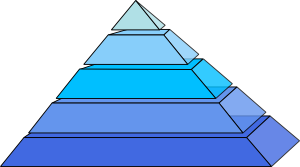
\includegraphics[width=1.1cm]{../Strukturfiler/FIGS/BluePyramid} & \begin{minipage}{\obsl}}{\end{minipage}\\ \end{tabular}\vspace{4mm}\newline}


% = Forudsætning = basis
\newenvironment{basis}{\begin{flushleft} \begin{itshape} }{\end{itshape} \end{flushleft}}


% = Opsummering =
\newenvironment{summary}{\clearpage\pagecolor{sumgul}\section{Opsummering}}{\newpage\pagecolor{white}}











% = Counter
\newcounter{opgavecount}[section]
\setcounter{opgavecount}{0}
\newcounter{spgcount}[opgavecount]
\setcounter{spgcount}{0}
\renewcommand{\thespgcount}{\alph{spgcount})}



% = EXERCISE = (DIVIDER)

\newcommand{\exercisebegin}[1][]{\bigskip\needspace{3\baselineskip}\refstepcounter{opgavecount}\titlegraphic{mingroen}\textcolor{mingroen}{\th{Opgave \theopgavecount \hspace*{1cm} #1}}\medskip\par}

% = QUIZEXERCISE = (DIVIDER)

\newcommand{\quizexercisebegin}[1][]{\bigskip\needspace{3\baselineskip}\refstepcounter{opgavecount}\titlegraphic{mingroen}\textcolor{mingroen}{\th{Quiz-Opgave \theopgavecount \hspace*{1cm} #1}}\medskip\par}

% = QUESTION =

\newenvironment{question}{\refstepcounter{spgcount}\begin{itemize}\item[\thespgcount]}{\end{itemize}\hspace*{\fill}}

% = VINK =

\newenvironment{vink}{\begin{tabular}{m{.9cm}<{\hspace*{2mm}}@{}|m{\obsl}@{}}\hspace*{-4pt}\raggedleft
\includegraphics[width=.9cm]{../Strukturfiler/FIGS/Think} & \begin{minipage}{\obsl}}{\end{minipage}\\ \end{tabular}\medskip\\}
	
% = FACIT =

\newenvironment{facit}{\begin{tabular}{m{.9cm}<{\hspace*{2mm}}@{}|m{\obsl}@{}}\hspace*{-4pt}\raggedleft
\includegraphics[width=.9cm]{../Strukturfiler/FIGS/Check} & \begin{minipage}{\obsl}}{\end{minipage}\\ \end{tabular}\medskip\\}








\newcommand{\afsnit}[1]{\bigskip\th{\titlegraphic{mingroen}\textcolor{mingroen}{#1}} \\ \rule[7pt]{.4\textwidth}{1pt} \vspace*{-2.5mm}\par}

% (DIVIDER):
\newcommand{\ugedagdatotitel}[4]{\pagebreak[4]\section{Semesteruge #1 -- #2 Dag \hspace*{1mm} (#3)} \vspace*{-4mm} \rule[5pt]{\textwidth}{1pt}\vspace*{-2.5mm} \begin{center}\large{\th{#4}}\end{center} \fancyhead[C]{\th{Semesteruge #1}}}

\newenvironment{skema}[1]{\definecolor{shadecolor}{rgb}{0.96,.98, 1.0} \setlength{\FrameSep}{6pt} \renewcommand{\FrameHeightAdjust}{10pt} \vspace*{-4pt}\begin{shaded} \begin{tabular}{#1}}{\end{tabular} \end{shaded} \vspace*{-7pt}}


% ========================

% MAKROER

%\newenvironment{matr}[1][]{\hspace*{-.8mm}\left[\hspace*{-1mm}\begin{array}{#1}}{\end{array}\hspace*{-1mm}\right]\hspace*{-.8mm}}
\newcommand{\bevisslut}{\begin{scriptsize} \begin{flushright} $ \blacksquare $ \end{flushright} \end{scriptsize}}

\newcommand{\tref}[2]{\hyperref[#1]{#2 \ref*{#1}}}
\newcommand{\thref}[2]{\hyperref[#1]{#2}}

\newcommand{\refA}[1]{\colorbox{yellow}{\ref{#1}}}
\newcommand{\hrefA}[2]{\colorbox{yellow}{\href{#1}{#2}}}
\newcommand{\trefA}[2]{\colorbox{yellow}{\hyperref[#1]{#2 \ref*{#1}}}}
\newcommand{\threfA}[2]{\colorbox{yellow}{\hyperref[#1]{#2}}}

\newenvironment{matr}[1]{\hspace*{-.8mm}\begin{bmatrix}\hspace*{-1mm}\begin{array}{#1}}{\end{array}\hspace*{-1mm}\end{bmatrix}\hspace*{-.8mm}}
\newcommand{\transp}{\hspace*{-.6mm}^{\top}}

\newcommand{\maengde}[2]{\left\lbrace \hspace*{-1mm} \begin{array}{c|c} #1 & #2 \end{array} \hspace*{-1mm} \right\rbrace}

\newenvironment{eqnalign}[1]{\setlength{\arraycolsep}{1.3pt}\begin{equation}\begin{array}{#1}}{\end{array}\end{equation}\par}
\newcommand{\eqnl}{\setlength{\arraycolsep}{1.3pt}}

\newcommand{\matind}[3]{{_\mathrm{#1}\mathbf{#2}_\mathrm{#3}}}
\newcommand{\vekind}[2]{{_\mathrm{#1}\mathbf{#2}}}
\newcommand{\jac}[2]{{\mathrm{Jacobi}_\mathbf{#1} (#2)}}
\newcommand{\diver}[2]{{\mathrm{div}\mathbf{#1} (#2)}}
\newcommand{\rot}[1]{{\mathbf{rot}\mathbf{(#1)}}}

\newcommand{\am}{\mathrm{am}}
\newcommand{\gm}{\mathrm{gm}}
\newcommand{\E}{\mathrm{E}}
\newcommand{\Span}{\mathrm{span}}
\newcommand{\mU}{\mathbf{U}}

\newcommand{\ms}{\medskip\\}
\newcommand{\bs}{\bigskip\\}

\newcommand{\mA}{\mathbf{A}}
\newcommand{\mB}{\mathbf{B}}
\newcommand{\mC}{\mathbf{C}}
\newcommand{\mD}{\mathbf{D}}
\newcommand{\mE}{\mathbf{E}}
\newcommand{\mF}{\mathbf{F}}
\newcommand{\mK}{\mathbf{K}}
\newcommand{\mI}{\mathbf{I}}
\newcommand{\mM}{\mathbf{M}}
\newcommand{\mN}{\mathbf{N}}
\newcommand{\mQ}{\mathbf{Q}}
\newcommand{\mT}{\mathbf{T}}
\newcommand{\mV}{\mathbf{V}}
\newcommand{\mW}{\mathbf{W}}
\newcommand{\mX}{\mathbf{X}}
\newcommand{\ma}{\mathbf{a}}
\newcommand{\mb}{\mathbf{b}}
\newcommand{\mc}{\mathbf{c}}
\newcommand{\md}{\mathbf{d}}
\newcommand{\me}{\mathbf{e}}
\newcommand{\mn}{\mathbf{n}}
\newcommand{\mr}{\mathbf{r}}
\newcommand{\mv}{\mathbf{v}}
\newcommand{\mw}{\mathbf{w}}
\newcommand{\mx}{\mathbf{x}}
\newcommand{\mxb}{\mathbf{x_{bet}}}
\newcommand{\my}{\mathbf{y}}
\newcommand{\mz}{\mathbf{z}}
\newcommand{\reel}{\mathbb{R}}
\newcommand{\mL}{\bm{\Lambda}} %Lambda-matrix
\newcommand{\mnul}{\bm{0}}
\newcommand{\trap}[1]{\mathrm{trap}(#1)}
\newcommand{\Det}{\operatorname{Det}}
\newcommand{\adj}{\operatorname{adj}}
\newcommand{\Ar}{\operatorname{Areal}}
\newcommand{\Vol}{\operatorname{Vol}}
\newcommand{\Rum}{\operatorname{Rum}}
\newcommand{\diag}{\operatorname{\bf{diag}}}
\newcommand{\bidiag}{\operatorname{\bf{bidiag}}}
\newcommand{\spanVec}[1]{\mathrm{span}\{#1\}}
\newcommand{\Div}{\operatorname{Div}}
\newcommand{\Rot}{\operatorname{\mathbf{Rot}}}

\newcommand{\Jac}{\operatorname{Jacobi}}
\newcommand{\Tan}{\operatorname{Tan}}
\newcommand{\Ort}{\operatorname{Ort}}
\newcommand{\Flux}{\operatorname{Flux}}
\newcommand{\Cmass}{\operatorname{Cm}}
\newcommand{\Imom}{\operatorname{Im}}
\newcommand{\Pmom}{\operatorname{Pm}}
\newcommand{\IS}{\operatorname{I}}
\newcommand{\IIS}{\operatorname{II}}
\newcommand{\IIIS}{\operatorname{III}}
\newcommand{\Le}{\operatorname{L}}
\newcommand{\app}{\operatorname{app}}
\newcommand{\M}{\operatorname{M}}
\newcommand{\re}{\mathrm{Re}}
\newcommand{\im}{\mathrm{Im}}

\newcommand{\compl}{\mathbb{C}} %de komplekse tal
\newcommand{\e}{\mathrm{e}} %eksponentialfunktionen. lodret 'e', og altså ikke kursiv ligesom andre bogstaver.





% Medialink: SCREEN: (QRcode) + thumbnail image + link på kodenummer (til qr.dtu.dk)
\newcommand{\onlinemedia}[3]{
	\begin{wrapfigure}{r}{3.2cm} 
		\vspace{-30pt} 
		\vspace{#1pt} 
		\begin{flushright} 
			\includegraphics[width=3cm]{qr/#2.png} 
			\tiny 
			\href{http://qr.dtu.dk/#2}{#2: #3}
			\normalsize  
		\end{flushright} 
		\vspace{-10pt} 
	\end{wrapfigure}
}
\newcommand{\onlinemediathumb}[3]{
	\begin{wrapfigure}{r}{3.2cm} 
		\vspace{-30pt} 
		\vspace{#1pt} 
		\begin{flushright} 
			\includegraphics[width=3cm]{qr/#2.png} 
			\includegraphics[width=3cm]{qr/#2_thumb.png} 
			\tiny 
			\href{http://qr.dtu.dk/#2}{#2: #3}
			\normalsize  
		\end{flushright} 
		\vspace{-10pt} 
	\end{wrapfigure}
}



% Index:
\usepackage{makeidx}
\makeindex
\newcommand\ind[2]{\index{#1}\textbf{\textit{\textcolor{black}{#2}}}}

% ###SERVER_EXCLUDE_BEGIN###
\externaldocument[NUID17-]{../../enoten/TN01-Talrum/Talrum}
\externaldocument[NUID1-]{../../enoten/TN02-Ligningssystemer/TNdriver}
\externaldocument[NUID2-]{../../enoten/TN03-Matricer_og_Matrixalgebra/Matricer_og_matrixalgebra}
\externaldocument[NUID3-]{../../enoten/TN04-Kvadratiske_matricer/TNdriver}
\externaldocument[NUID11-]{../../enoten/TN05-Determinanter/Determinanter}
\externaldocument[NUID12-]{../../enoten/TN06-GeometriskeVektorer/GeometriskeVektorer}
\externaldocument[NUID18-]{../../enoten/TN07-Vektorrum/VektorRum}
\externaldocument[NUID21-]{../../enoten/TN08-LinAfbildninger/LinAfbildninger}
\externaldocument[NUID23-]{../../enoten/TN09-Egenvaerdier_og_egenvektorer/TNdriver}
\externaldocument[NUID24-]{../../enoten/TN10-Diagonalisering_med_egenvektorer/TNdriver}
\externaldocument[NUID10-]{../../enoten/TN11-1.ordens_differentialligninger/TNdriver}
\externaldocument[NUID13-]{../../enoten/TN12-1.ordens_differentialligningssystemer/TNdriver}
\externaldocument[NUID14-]{../../enoten/TN13-2.ordens_differentialligninger/TNdriver}
\externaldocument[NUID27-]{../../enoten/TN14-Elemenataere_funktioner/Elementaere_Funktioner}
\externaldocument[NUID28-]{../../enoten/TN15-Funktioner2Variable/Funktioner_To_Variable}
\externaldocument[NUID29-]{../../enoten/TN16-Gradienter_og_Tangentplaner/Gradienter_og_Tangentplaner}
\externaldocument[NUID32-]{../../enoten/TN17-Taylor_formler/Taylor_Formler}
\externaldocument[NUID33-]{../../enoten/TN18-Taylor_2Var/Taylor_2Var}
\externaldocument[NUID34-]{../../enoten/TN19-SymMat/SymmetriskeMatricer}
\externaldocument[NUID35-]{../../enoten/TN20-KegleSnit/Keglesnit}
\externaldocument[NUID36-]{../../enoten/TN21-Riemann_Integral/Riemann_01}
\externaldocument[NUID37-]{../../enoten/TN22-Plan_Int/Plan_Int_01}
\externaldocument[NUID39-]{../../enoten/TN23-Flade_Int/Flade_Rum_Int_01}
\externaldocument[NUID40-]{../../enoten/TN24-Vektorfelter/Vektorfelter_01}
\externaldocument[NUID41-]{../../enoten/TN25-Flux/Flux_02}
\externaldocument[NUID42-]{../../enoten/TN26-Gauss/Gauss_01}
\externaldocument[NUID128-]{../../enoten/TN27-Stokes/Stokes_01}
\externaldocument[NUID43-]{../../enoten/TN29-KomplekseTal/KomplekseTal}

\externaldocument[NUID6-]{../../E-math-opgaver/Opgaver/opgU123}
\externaldocument[NUID19-]{../../E-math-opgaver/Opgaver/opgU45}
\externaldocument[NUID20-]{../../E-math-opgaver/Opgaver/opgU678}
\externaldocument[NUID25-]{../../E-math-opgaver/Opgaver/opgU910SD}
\externaldocument[NUID31-]{../../E-math-opgaver/OpgaverF11-U123/opgF123}
% \externaldocument[NUID9-]{../../E-math-opgaver/Opgaver/Dagsordner E10}
% ###SERVER_EXCLUDE_END###


% Begin document and set alternative chapter title:
\begin{document}
\renewcommand{\chaptername}{eNote}

\setcounter{chapter}{25} %SÆT DETTE TAL TIL 1 MINDRE END DET AKTUELLE TRANSFERNOTE-NUMMER!!

%%%%%%%%%%%%55%%%%%%%%%%%%%%%%%%%%%%%%%%%%%%%%%
%%%%%%%%%%%%%%%%%%%%%%%%%%%%%%%%%%%%%%%%%%%%%
%%% HERFRA SKAL DU SKRIVE ELLER INDSÆTTE %%%%
%%% DEN FIL DU ØNSKER %%%%%%%%%%%%%%%%%%%%%%%
%%%%%%%%%%%%%%%%%%%%%%%%%%%%%%%%%%%%%%%%%%%%%
%%%%%%%%%%%%%%%%%%%%%%%%%%%%%%%%%%%%%%%%%%%%%

% REF: TransferNote \ref{TN4-tn4} \nameref{TN4-tn4}
%
% \tref{NUID14-thm.koma}{sætning} \tref{NUID28-tn15}{eNote}
%
%\tref{NUID34-tn19}{eNote} Symmetriske matricer
%\tref{NUID33-tn18}{eNote} Taylor i 2 variable
%
% 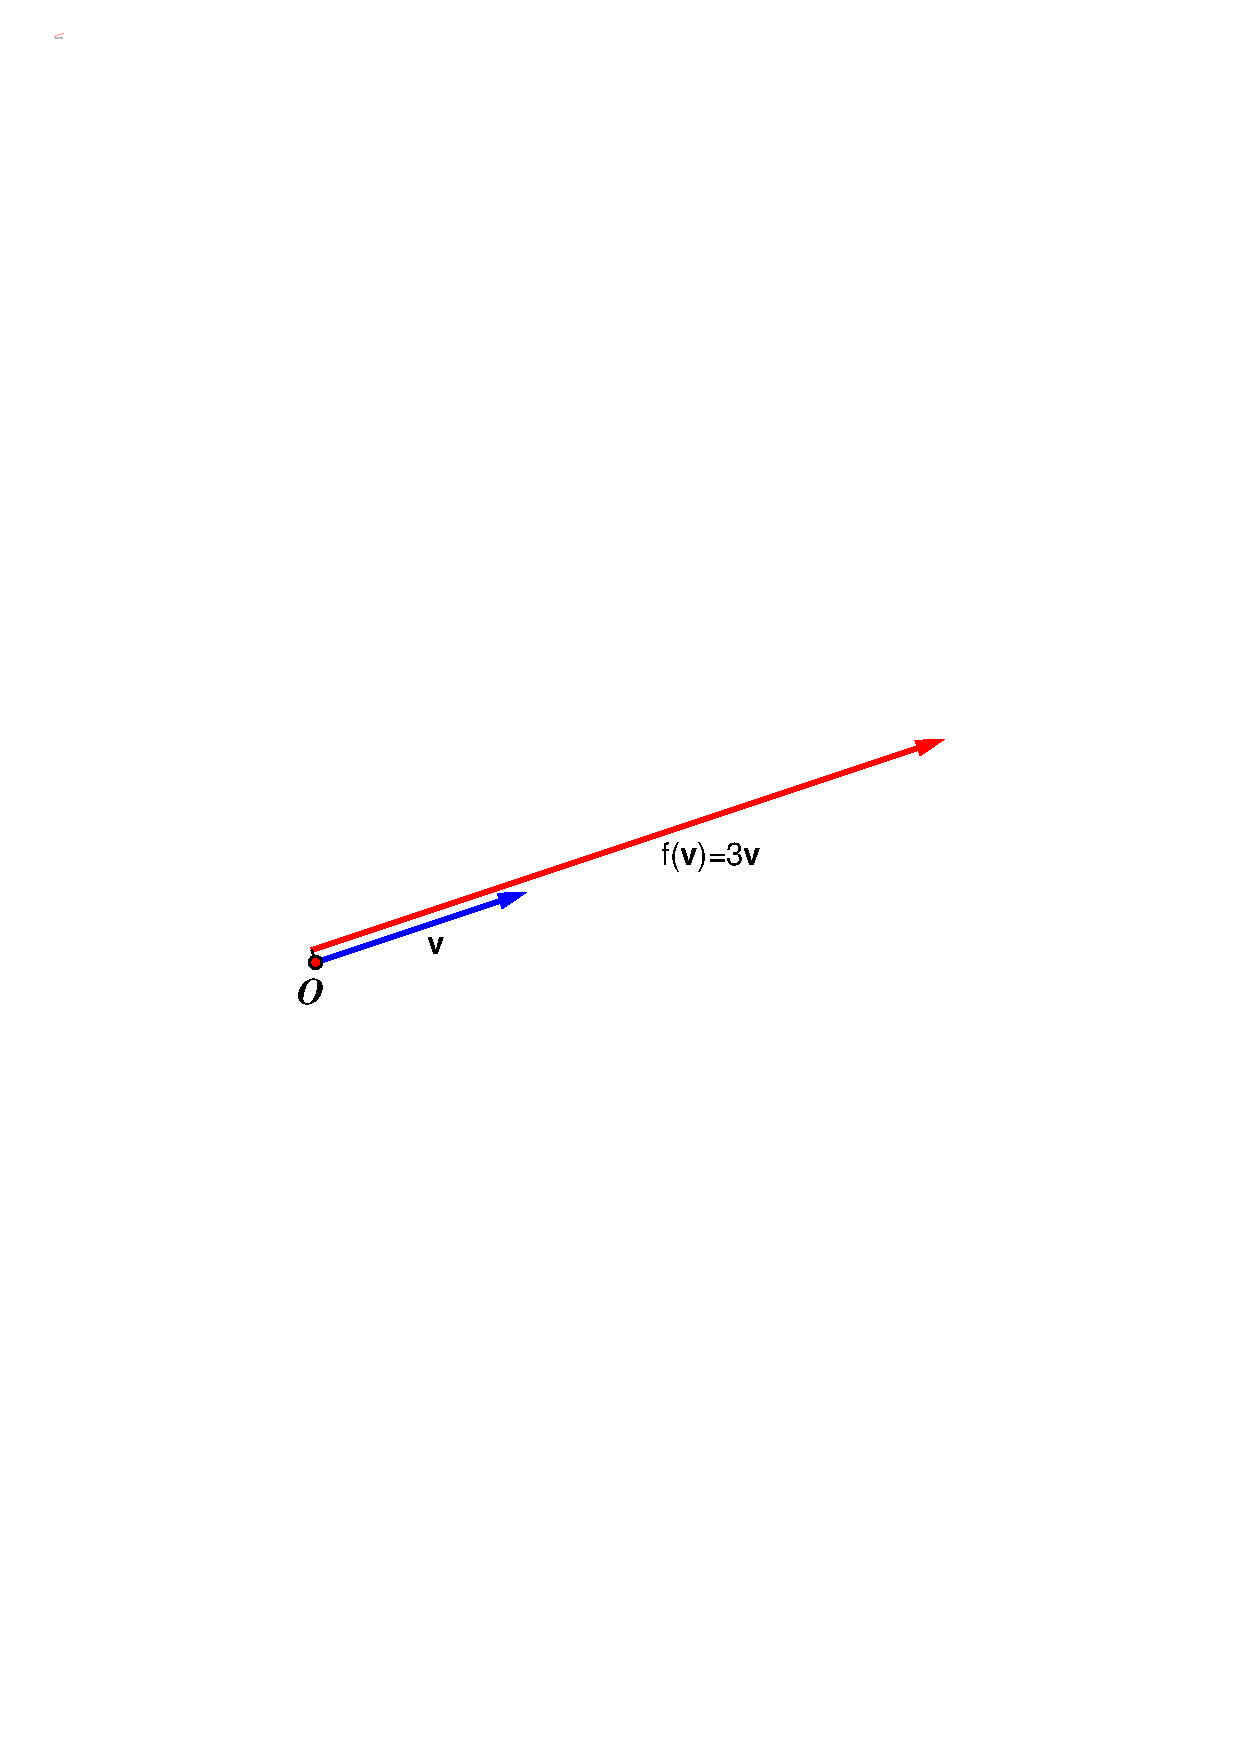
\includegraphics[trim=5cm 12cm 5cm 12cm,width=0.40\textwidth,clip]{skalering.pdf}
%
%\begin{equation}
%\matind vMa \cdot \matind aFa \cdot \matind aMv = \matind vFv \, ,
%\end{equation}
%hvor
%\begin{equation}
%\matind aMv = \begin{matr}{cccc} \vekind av_1 & \vekind av_2 & \cdots & \vekind av_n \end{matr} \quad \mathrm{og} \quad %\matind vFv = \diag(\lambda_1, \lambda_2, \ldots, \lambda_n) \, .
%\end{equation}
%
%$\vekind{e}{F}$
%$\matind{e}{F}{w}$
%
%\href{http://www-groups.dcs.st-and.ac.uk/~history/}{http://www-groups.dcs.st-and.ac.uk/~history/}

%%%%%%%%%%%%%%%%%%%%%%%%%%%%%%%%%%%%%%%%%%%%%%%%%%%
%%%%%%%%%%%%%%%%%%%%%%%%%%%%%%%%%%%%%%%%%%%%%%%%%%%
%%%%%%%%%%%%%%%%%%%%%%%%%%%%%%%%%%%%%%%%%%%%%%%%%%%
%%%%%%%%%%%%%%%%%%%%%%%%%%%%%%%%%%%%%%%%%%%%%%%%%%%

\chapter{Gauss' divergenssætning} \label{tn26}


\begin{basis}
I denne eNote vil vi bruge flowkurver for vektorfelter til at undersøge hvordan
overfladen af et rumligt område deformeres ved flowet og dermed afspejler en tilsvarende ændring i rumfanget af det område, der begrænses af overfladen.
Vi får derfor brug for at kende til analysen af vektorfelter fra \tref{NUID40-tn24}{eNote} samt flade- og rum-integraler fra \tref{NUID39-tn23}{eNote}.
Vi skal se, at divergensen af vektorfeltet er den lokale 'motor' for volumenændring. Hvis vi derfor integrerer divergensen over hele det rumlige område så får vi den totale øjeblikkelige volumen-ekspansion (med fortegn).
Hvis vektorfeltet er overalt eksploderende (med positiv divergens) så vokser rumfanget af ethvert rumligt område, hvis vektorfeltet er imploderende alle steder (med negativ divergens)  så aftager rumfanget af ethvert rumligt  område, der flyder med flowkurverne for vektorfeltet. \\

Alternativt kan man i stedet holde øje med om overfladen af et rumligt område er lokalt ekspanderende udad eller lokalt sammentrækkende indad i forhold til det rumlige område. Det gør vi  præcis med det ortogonale fladeintegral af vektorfeltet over overfladen -- et integral som også kaldes fluxen. \\
Dermed har vi to muligheder for at beregne ekspansion eller sammentrækning af et givet rumligt område når det flyder langs flowkurverne for vektorfeltet. Og de giver præcis det samme resultat -- det er indholdet af Gauss' divergenssætning.
\end{basis}




%%%%%%%%%%%%%%%%%%%%%%%%%%%%%%%%%%%%%%%%%%%%%%%%%%%
%%%%%%%%%%%%%%%%%%%%%%%%%%%%%%%%%%%%%%%%%%%%%%%%%%%
%%%%%%%%%%%%%%%%%%%%%%%%%%%%%%%%%%%%%%%%%%%%%%%%%%%
%%%%%%%%%%%%%%%%%%%%%%%%%%%%%%%%%%%%%%%%%%%%%%%%%%%
%%%%%%%%%%%%%%%%%%%%%%%%%%%%%%%%%%%%%%%%%%

\section{Det ortogonale fladeintegral, fluxen} \label{secFlux}

Lad ${\bf V}(x,y,z)$ være et glat vektorfelt i rummet, se \tref{NUID40-tn24}{eNote} og lad $F_{\bf r}$ betegne en glat parametriseret flade:
\begin{equation}
F_{\bf r}\quad : \quad \mathbf{r}(u,v) = (x(u,v), y(u,v), z(u,v))\quad , \quad (u,v) \in [a,b] \times [c,d] \quad .
\end{equation}
Ligesom ved konstruktionen af kurveintegralerne i \tref{NUID41-tn25}{eNote} har vi så i ethvert punkt på fladen \emph{to} veldefinerede vektorer, dels vektorfeltets værdi i punktet, $\mathbf{V}(\mathbf{r}(u,v))$, og dels normalvektoren ${\bf
r}'_{u}(u,v)\times{\bf r}'_{v}(u,v)$ til fladen i punktet. Det er ved hjælp af disse to vektorer vi vil konstruere fluxen af vektorfeltet igennem fladen.\\


Det {\em{orto\-gonale fladeintegral}} af ${\bf
V}(x,y,z)$ langs en given parametriseret flade $F_{\bf r}$ -- også kaldet  \emph{fluxen} af ${\bf
V}(x,y,z)$ igennem $F_{\bf r}$ --  er
fladeintegralet af projektionen (med fortegn) af ${\bf V}({\bf
r}(u,v))$ på fladens normal repræsenteret ved den standard enhedsvektor ${\mathbf{n}}_{F}$
der er proportional med og i samme retning som krydsproduktet
$\mathbf{N}_{F}(u,v) = {\bf r}'_{u}(u,v)\times {\bf r}'_{v}(u,v)$.

\begin{definition}[Fluxen af et vektorfelt] \label{defFlux}
Det ortogonale fladeintegral af vektorfeltet $\mathbf{V}(x,y,z)$ langs en parametriseret flade $F_{\bf r}$ , dvs.
fluxen af vektorfeltet igennem fladen,
er defineret ved
\begin{equation}
\Flux({\bf V}, F_{\bf r})\, = \,
\int_{F_{\bf r}}{\bf V} \bm{\cdot} {\mathbf{n}}_{F}\,d\mu \quad .
\end{equation}
\end{definition}

Integranden  i det
fladeintegral, der giver fluxen,  er altså givet ved skalarproduktet
\begin{equation}
f({\bf r}(u,v)) \, = \, {\bf V}({\bf r}(u,v)) \bm{\cdot} {\mathbf{n}}_{F}(u,v)
\quad ,
\end{equation}
hvor ${\mathbf{n}}_{F}(u,v)$ er defineret ved
\begin{equation}
{\mathbf{n}}_{F}(u,v)\, = \,
\begin{cases}
&{\bf r}'_{u}(u,v)\times{\bf r}'_{v}(u,v)/ \Vert {\bf
r}'_{u}(u,v)\times{\bf r}'_{v}(u,v) \Vert  \quad \text{hvis}\quad {\bf
r}'_{u}(u,v)\times{\bf r}'_{v}(u,v)\, \neq \,
{\bf 0} \\
&{\bf 0} \quad \text{hvis} \quad {\bf r}'_{u}(u,v)\times{\bf
r}'_{v}(u,v)\, = \, {\bf 0}
\end{cases}
\end{equation}
Fluxen af ${\bf V}(x,y,z)$ gennem $F_{\bf r}$ i
retningen $\,{\mathbf{n}}_{F}\,$ er derfor relativt
simpel at udregne - vi behøver ikke først at
finde længden af ${\bf r}'_{u}(u,v)\times{\bf
r}'_{v}(u,v)$ (jævnfør omformningen af det
tangentielle kurveintegral):
\begin{equation} \label{eqOrt}
\begin{aligned}
\Flux({\bf V}, F_{\bf r})\,&= \,
\int_{F_{\bf r}}{\bf V}\bm{\cdot} {\mathbf{n}}_{F}\,d\mu \,  \,\\
&= \, \int_{c}^{d}\int_{a}^{b}\left({\bf V}({\bf r}(u,v))\bm{\cdot} {\mathbf{n}}_{F}(u,v)\right) \,
 \Jac_{{\bf r}}(u,v)\,du \, dv \,\\
 &= \, \int_{c}^{d}\int_{a}^{b}\left({\bf
V}({\bf r}(u,v))\bm{\cdot} {\mathbf{n}}_{F}(u,v)\right) \,  \Vert {\bf
r}'_{u}(u,v)\times{\bf
r}'_{v}(u,v) \Vert \,du \, dv \,\\
 &=
\, \int_{c}^{d}\int_{a}^{b}{\bf V}({\bf r}(u,v))\bm{\cdot} ({\bf
r}'_{u}(u,v)\times{\bf r}'_{v}(u,v))\,du \, dv  \\
&= \, \int_{c}^{d}\int_{a}^{b}{\bf V}({\bf r}(u,v)) \bm{\cdot} \mathbf{N}_{F}(u,v) \,\,du \, dv  \quad .
\end{aligned}
\end{equation}

\begin{think}
Bemærk, at den sidste integrand i (\ref{eqOrt}) er kontinuert
og dermed integrabel, selv om det ikke umiddelbart fremgår af
definitionen,  idet vektorfeltet ${\mathbf{n}}_{F}(u, v)$ ikke
nødvendigvis er kontinuert - medmindre ${\bf r}(u, v)$ er en regulær
parameterfremstilling.
\end{think}

Vi har dermed et simpelt direkte udtryk for flux-beregninger:

\begin{theorem}[Fluxen, det ortogonale fladeintegral] \label{thmFluxBeregn}
Det ortogonale fladeintegral af $\mathbf{V}(x,y,z)$ over fladen $F_{\mathbf{r}}$, altså fluxen af $\mathbf{V}(x,y,z)$ igennem $F_{\mathbf{r}}$, beregnes således:
\begin{equation}
\begin{aligned}
\Flux({\bf V}, F_{\bf r})\,&= \, \int_{c}^{d}\int_{a}^{b}{\bf V}({\bf r}(u,v)) \bm{\cdot} ({\bf
r}'_{u}(u,v)\times{\bf r}'_{v}(u,v))\,du \, dv  \\
&= \, \int_{c}^{d}\int_{a}^{b}{\bf V}({\bf r}(u,v)) \bm{\cdot} \mathbf{N}_{F}(u,v)\,\,du \, dv  \quad .
\end{aligned}
\end{equation}
\end{theorem}

\begin{aha}
Læg mærke til, at hvis en flade $F_{\bf r}$  parametriseres med en anden parametrisering $\widehat{F}_{\,\widehat{\mathbf{r}}}$ som
giver den modsat rettede standard enhedsnormalvektor $\mathbf{n}_{\widehat{F}}$ i ethvert punkt på fladen:
$\mathbf{n}_{\widehat{F}}(\widehat{u}, \widehat{v}) = -\mathbf{n}_{F}(u,v)$, hvor $\mathbf{r}(u,v) = \widehat{\mathbf{r}}(\widehat{u}, \widehat{v})$,
så skifter fluxen fortegn:
\begin{equation}
\Flux(\mathbf{V}, \widehat{F}_{\,\widehat{\mathbf{r}}}) = - \Flux(\mathbf{V}, F_{\mathbf{r}}) \quad.
\end{equation}
\end{aha}

\begin{think}
Det ortogonale kurveintegral er kort indført som et dualt begreb i forhold til det mere naturlige tangentielle kurveintegral i \tref{NUID41-tn25}{eNote}. Det duale begreb i forhold til det ovenfor indførte naturlige ortogonale fladeintegral er det \emph{tangentielle fladeintegral} af et givet vektorfelt over en given flade.
\end{think}

\begin{definition}[Det tangentielle fladeintegral] \label{defTangFladeInt}
I analogi med det ortogonale fladeintegral, fluxen,  definerer vi det {\em
tangentielle} fladeintegral, som vi vil kalde  $\Tan({\bf V},
F_{\bf r})$ af ${\bf V}$ over fladen $F_{\bf r}$,
ved at projicere ${\bf V}({\bf r}(u,v))$
vinkelret ind på tangentplanen til $F_{\bf r}$
(udspændt af ${\bf r}'_{u}(u,v)$ og ${\bf
r}'_{v}(u,v)$ i punktet ${\bf r}(u,v)$) og
dernæst finde fladeintegralet af længden af denne
projektion (som funktion af $(u, v)$).
\end{definition}



\begin{figure}[h]
\centerline{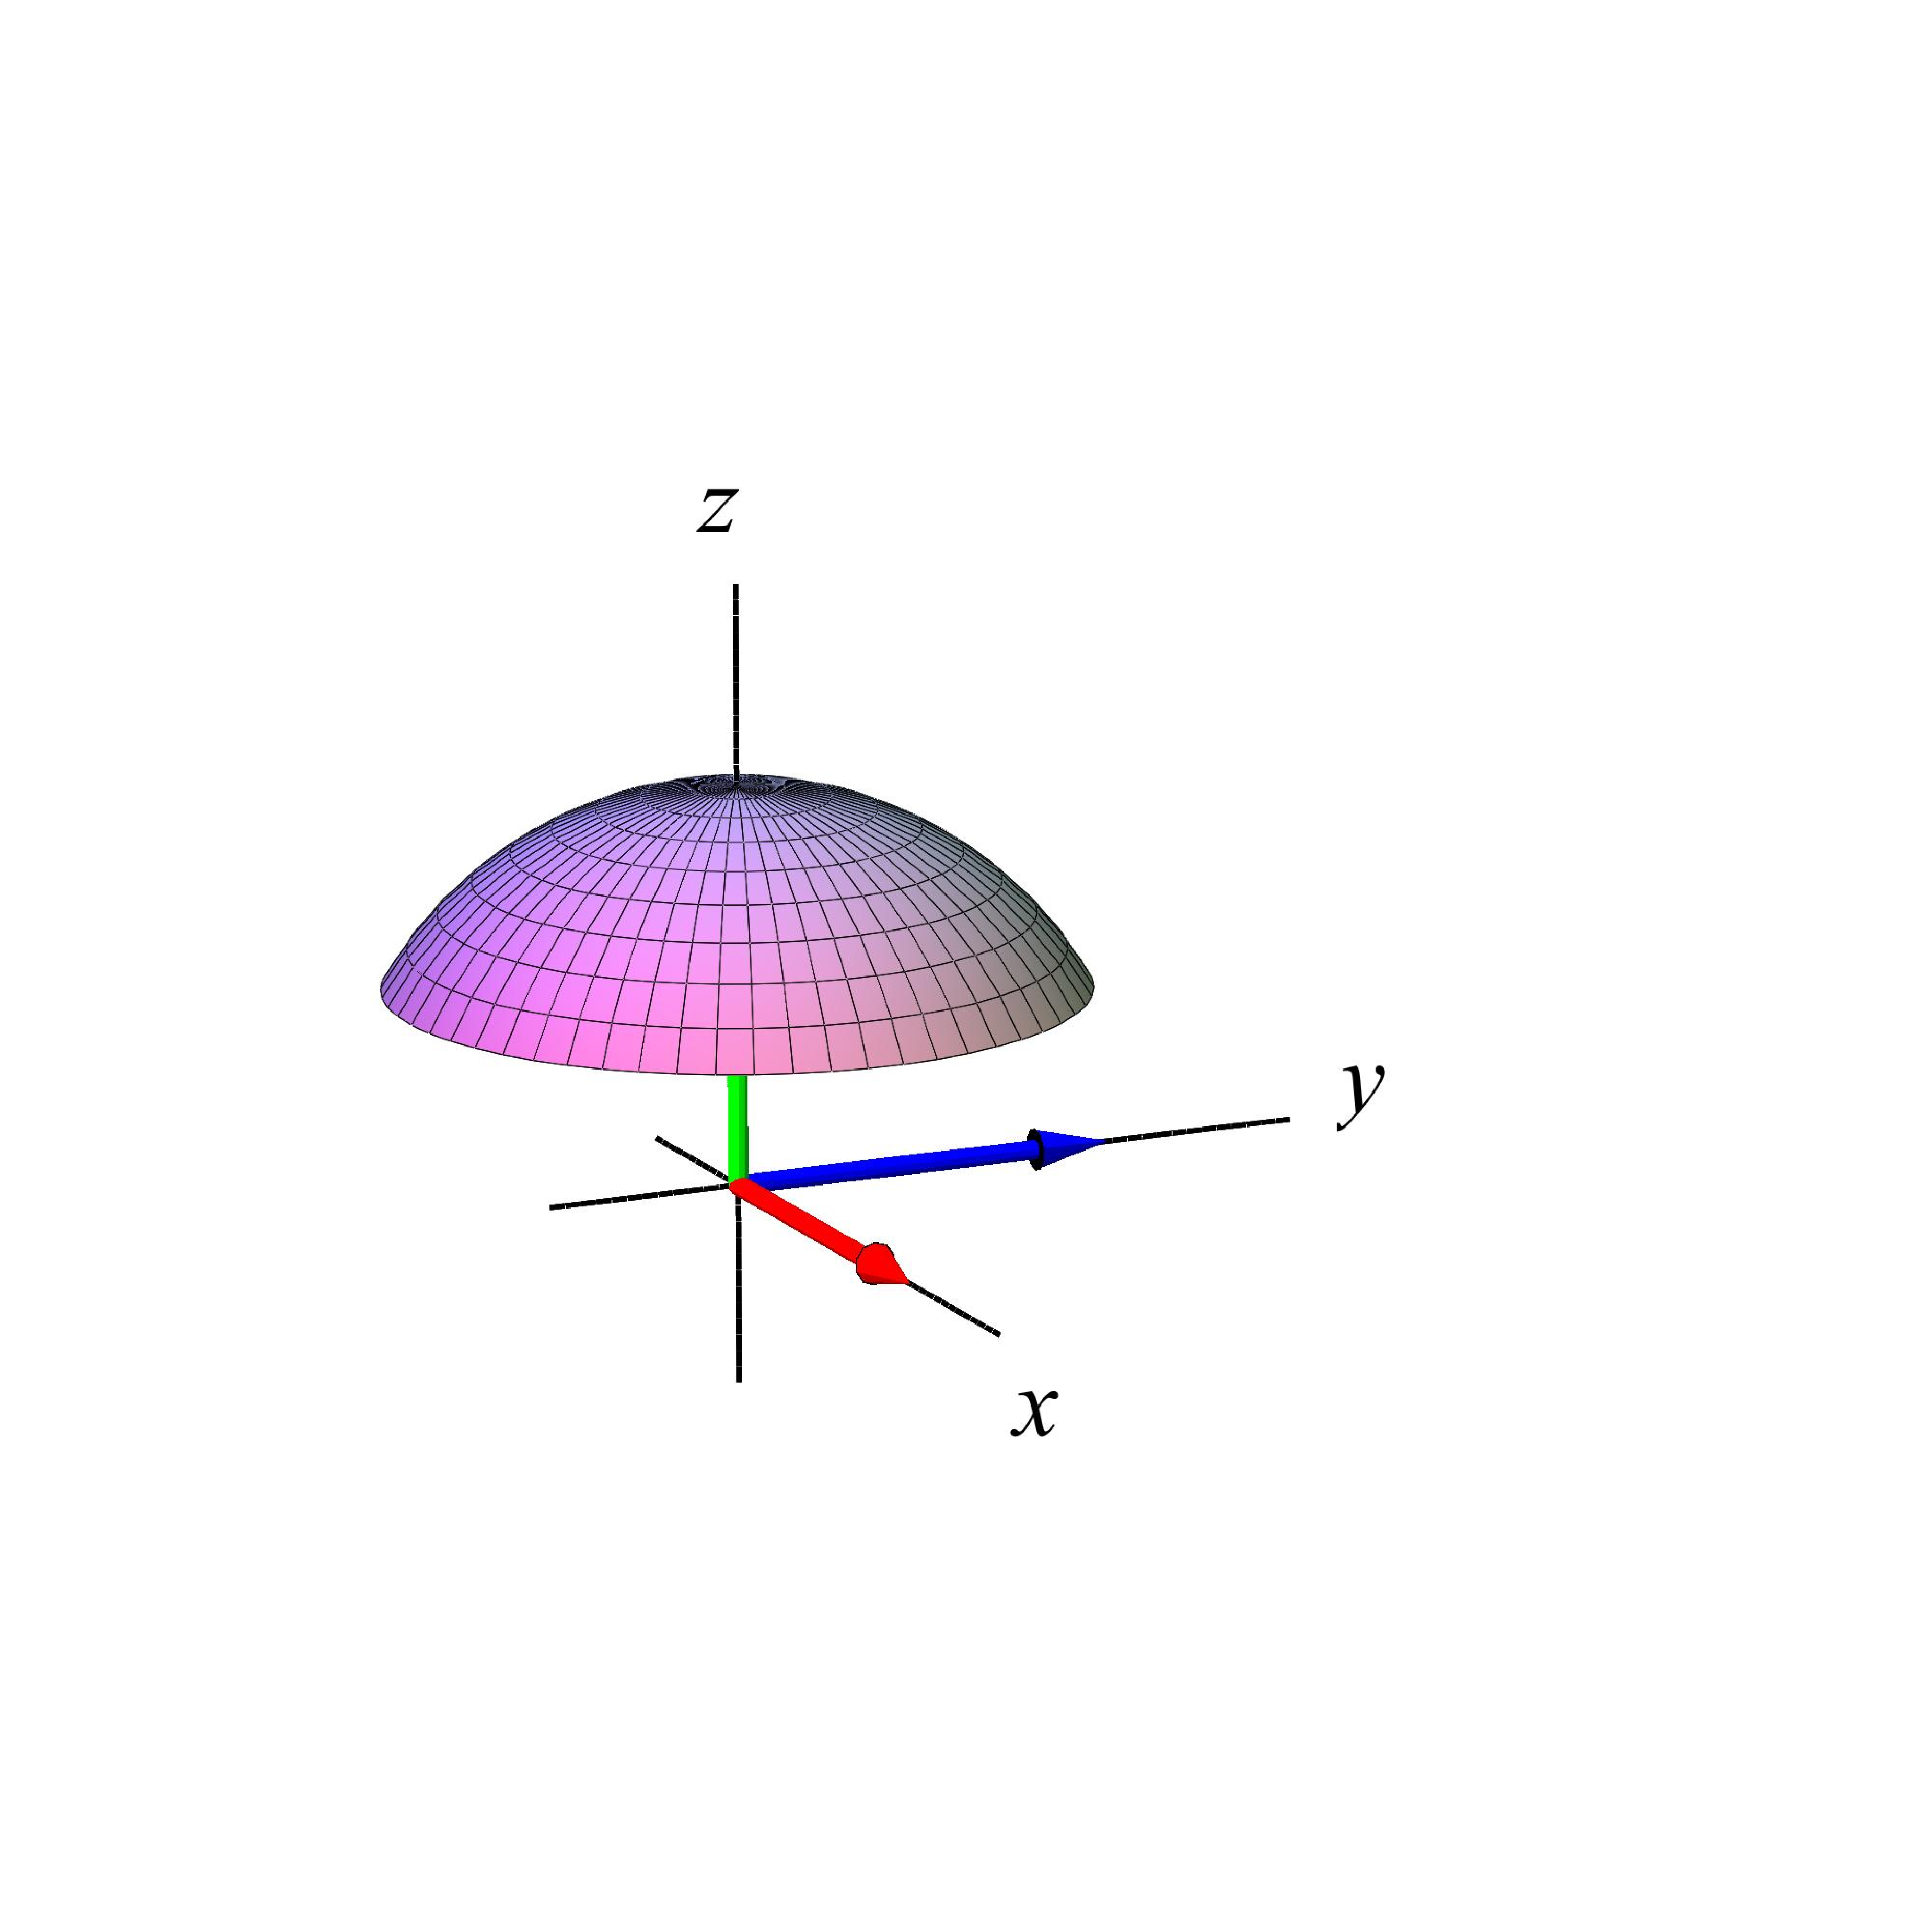
\includegraphics[width=70mm]{FIGS/plotKalotA1}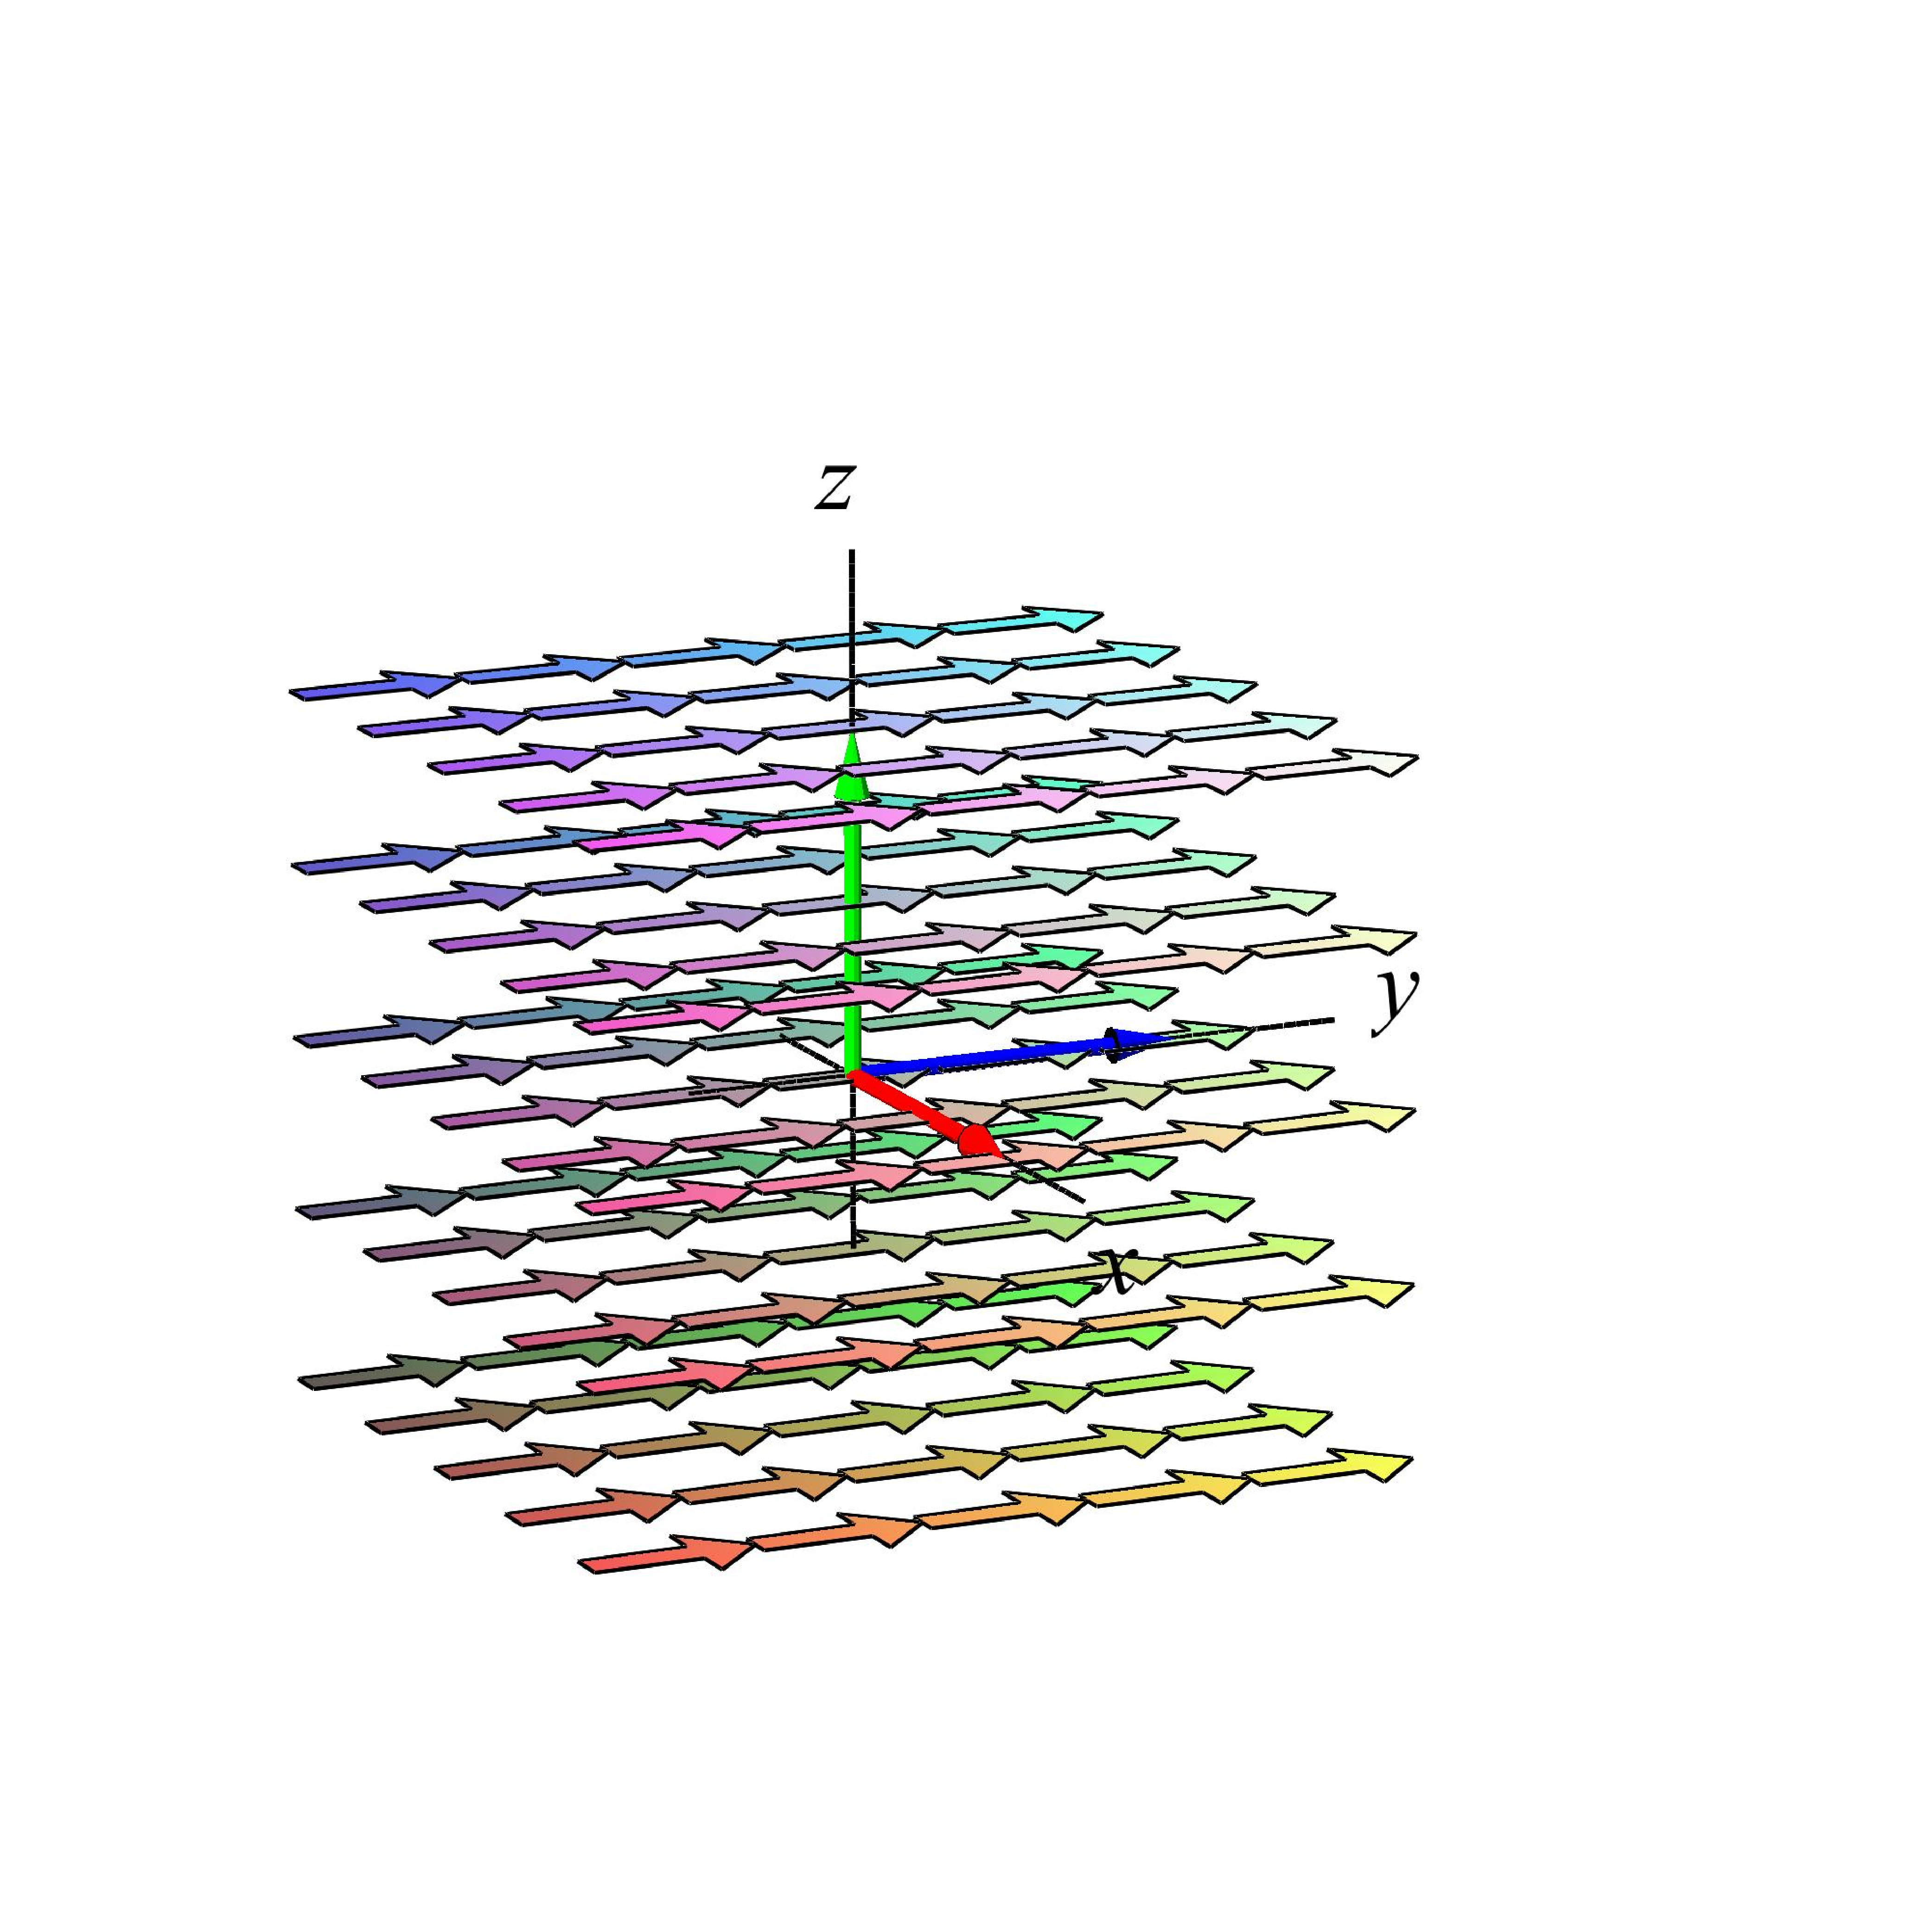
\includegraphics[width=70mm]{FIGS/plotKalotB2}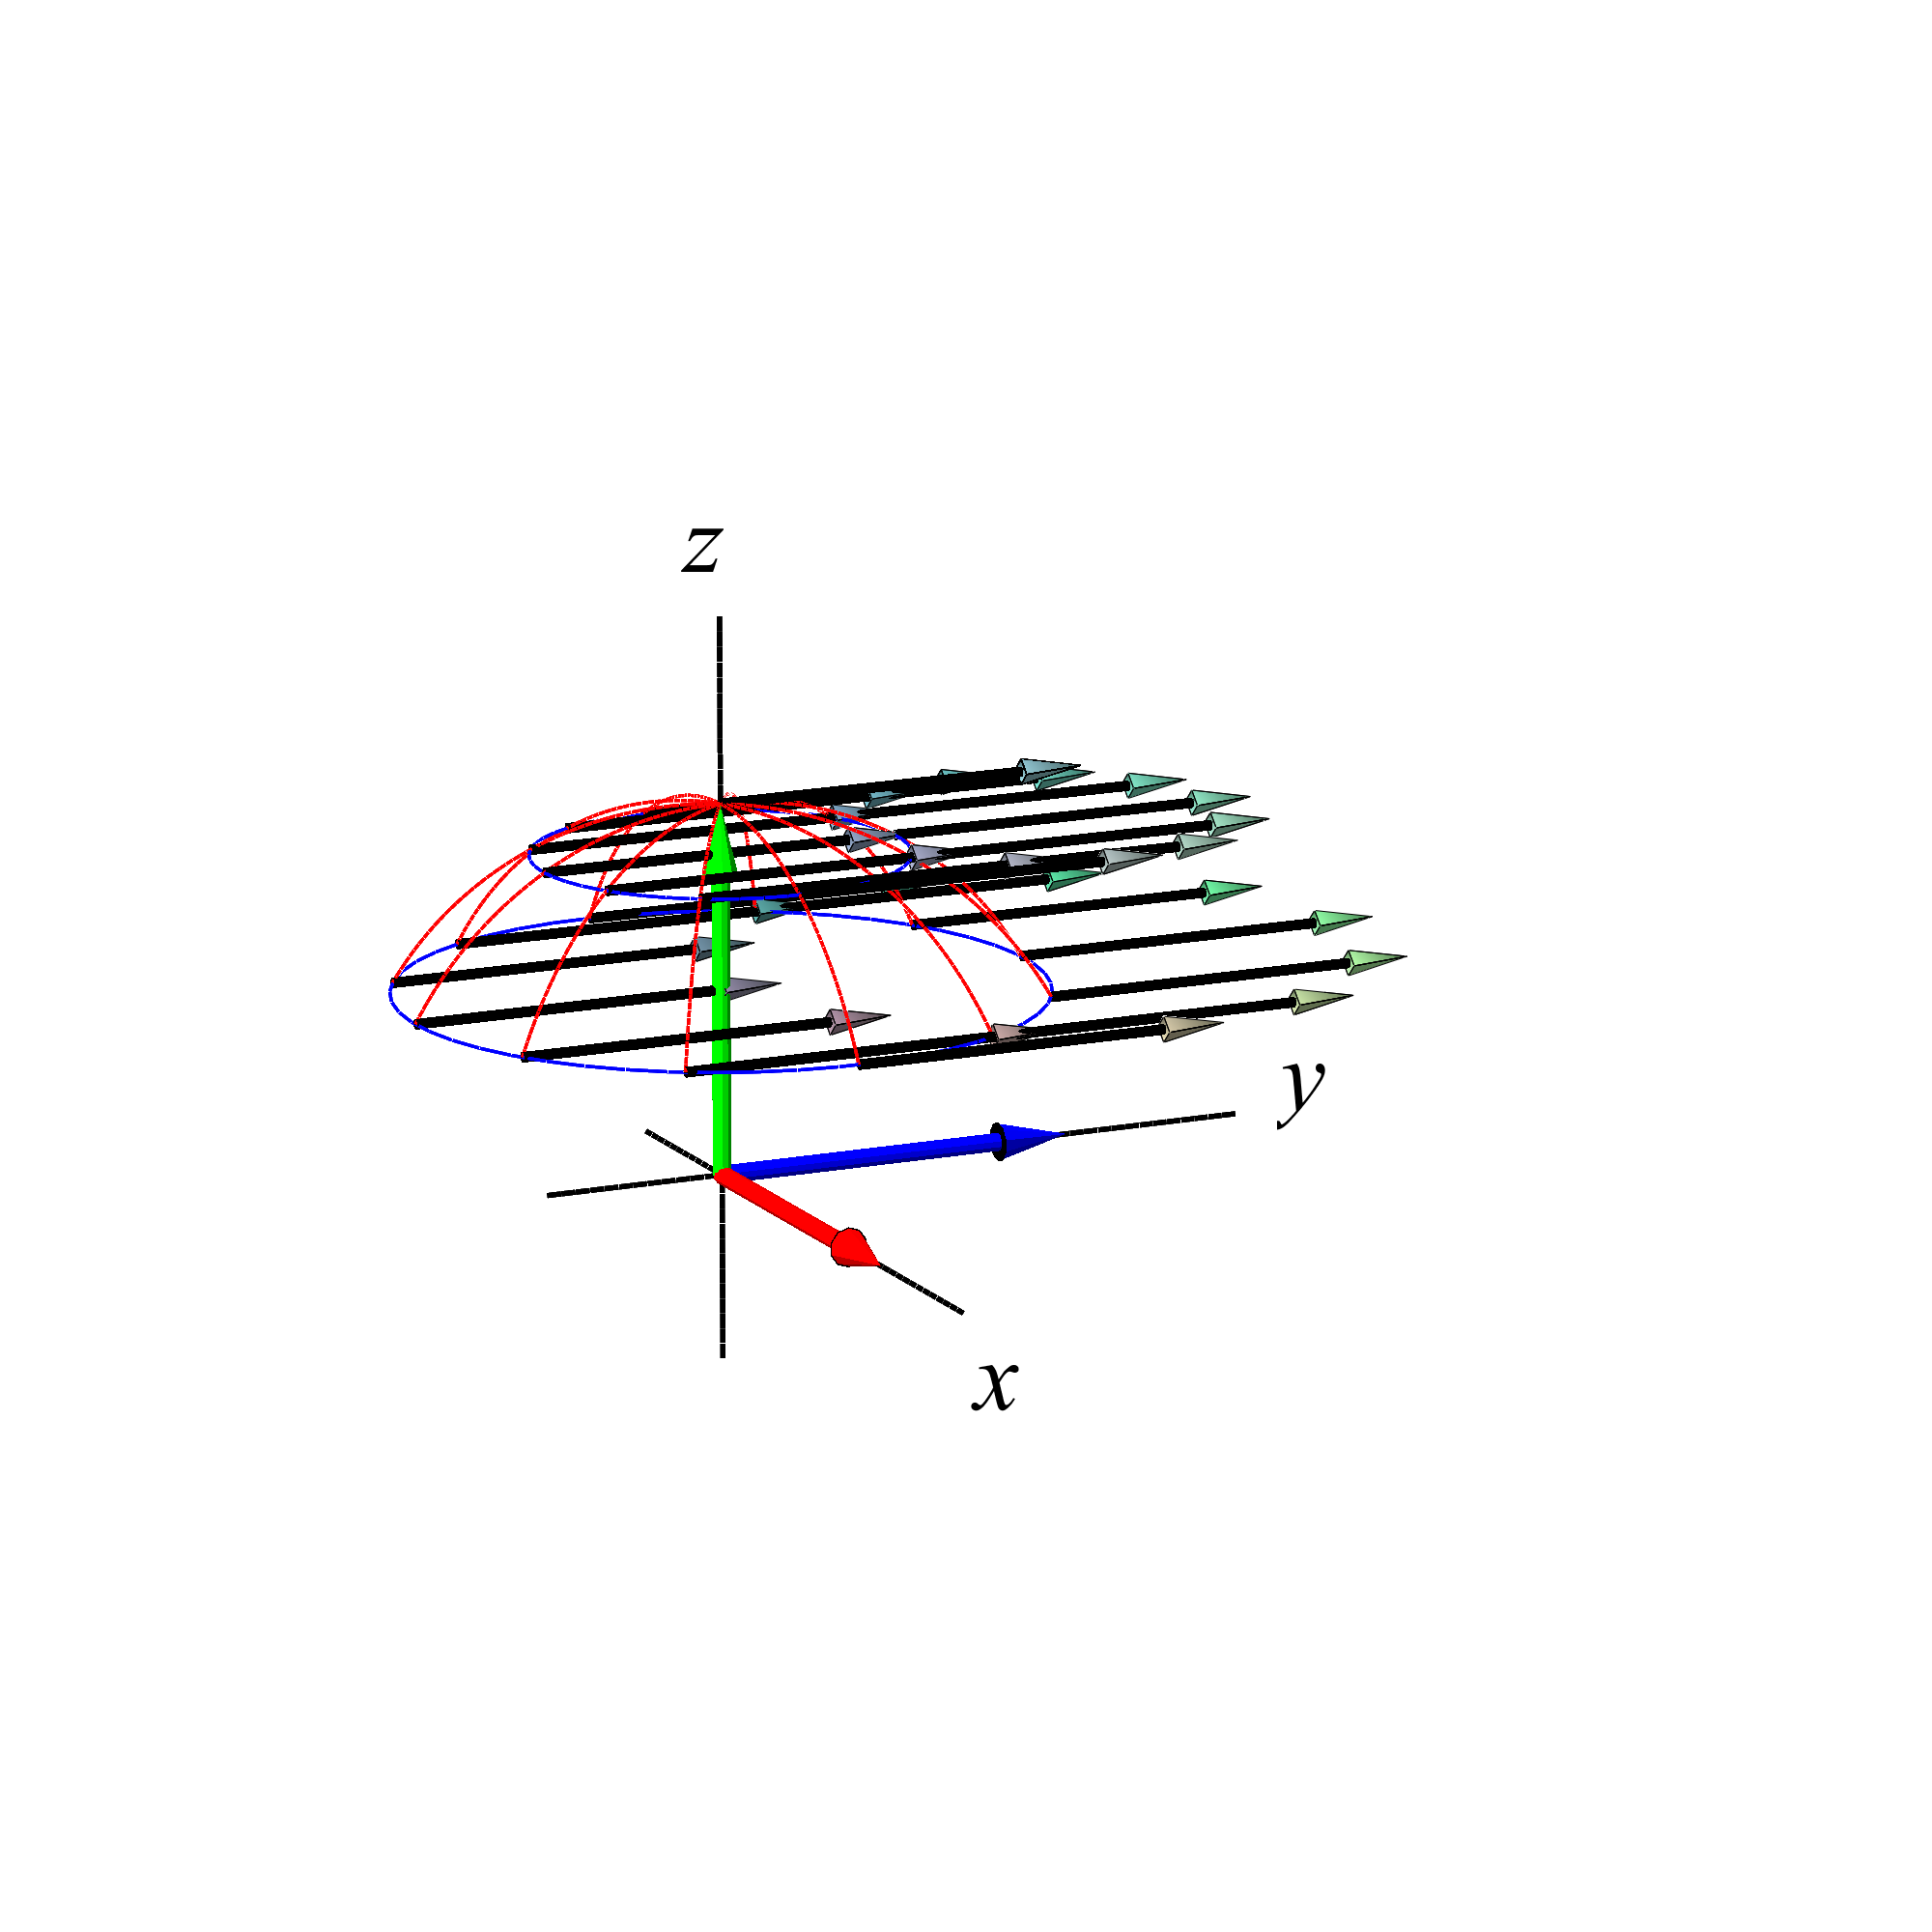
\includegraphics[width=70mm]{FIGS/plotKalotB3}}
\begin{center}
\caption{\small{Denne kalot af en kugleflade er
givet ved parameterfremstillingen ${\bf r}(u, v)
\, = \, (\sin(u)\cos(v), \sin(u)\sin(v), \cos(u)
) \,\,, \,\, u \in [0, \frac{\pi}{3}]\,\, , \, \,
v \in [-\pi, \pi]\, $. Vektorfeltet er givet ved
${\bf V}(x,y,z) \, = \, (0, 1,0)$.}} \label{figKalot12}
\end{center}
\end{figure}

\begin{exercise}
Vedrørende figurerne \ref{figKalot12} og \ref{figKalotA12}:
\begin{enumerate}
\item Bestem det tangentielle
fladeintegral for hver af vektorfelteterne ${\bf V}(x,y,z)\,
= \, (0, 1, 0)$ og ${\bf V}(x,y,z)\,
= \, (1/\sqrt{5}, 0, -2/\sqrt{5})$   langs kuglekalotten.
\item Bestem de respektive ortogonale fladeintegraler (fluxene) for hver af
vektorfelterne igennem kuglekalotten.
\end{enumerate}
\end{exercise}


\begin{figure}[h]
\centerline{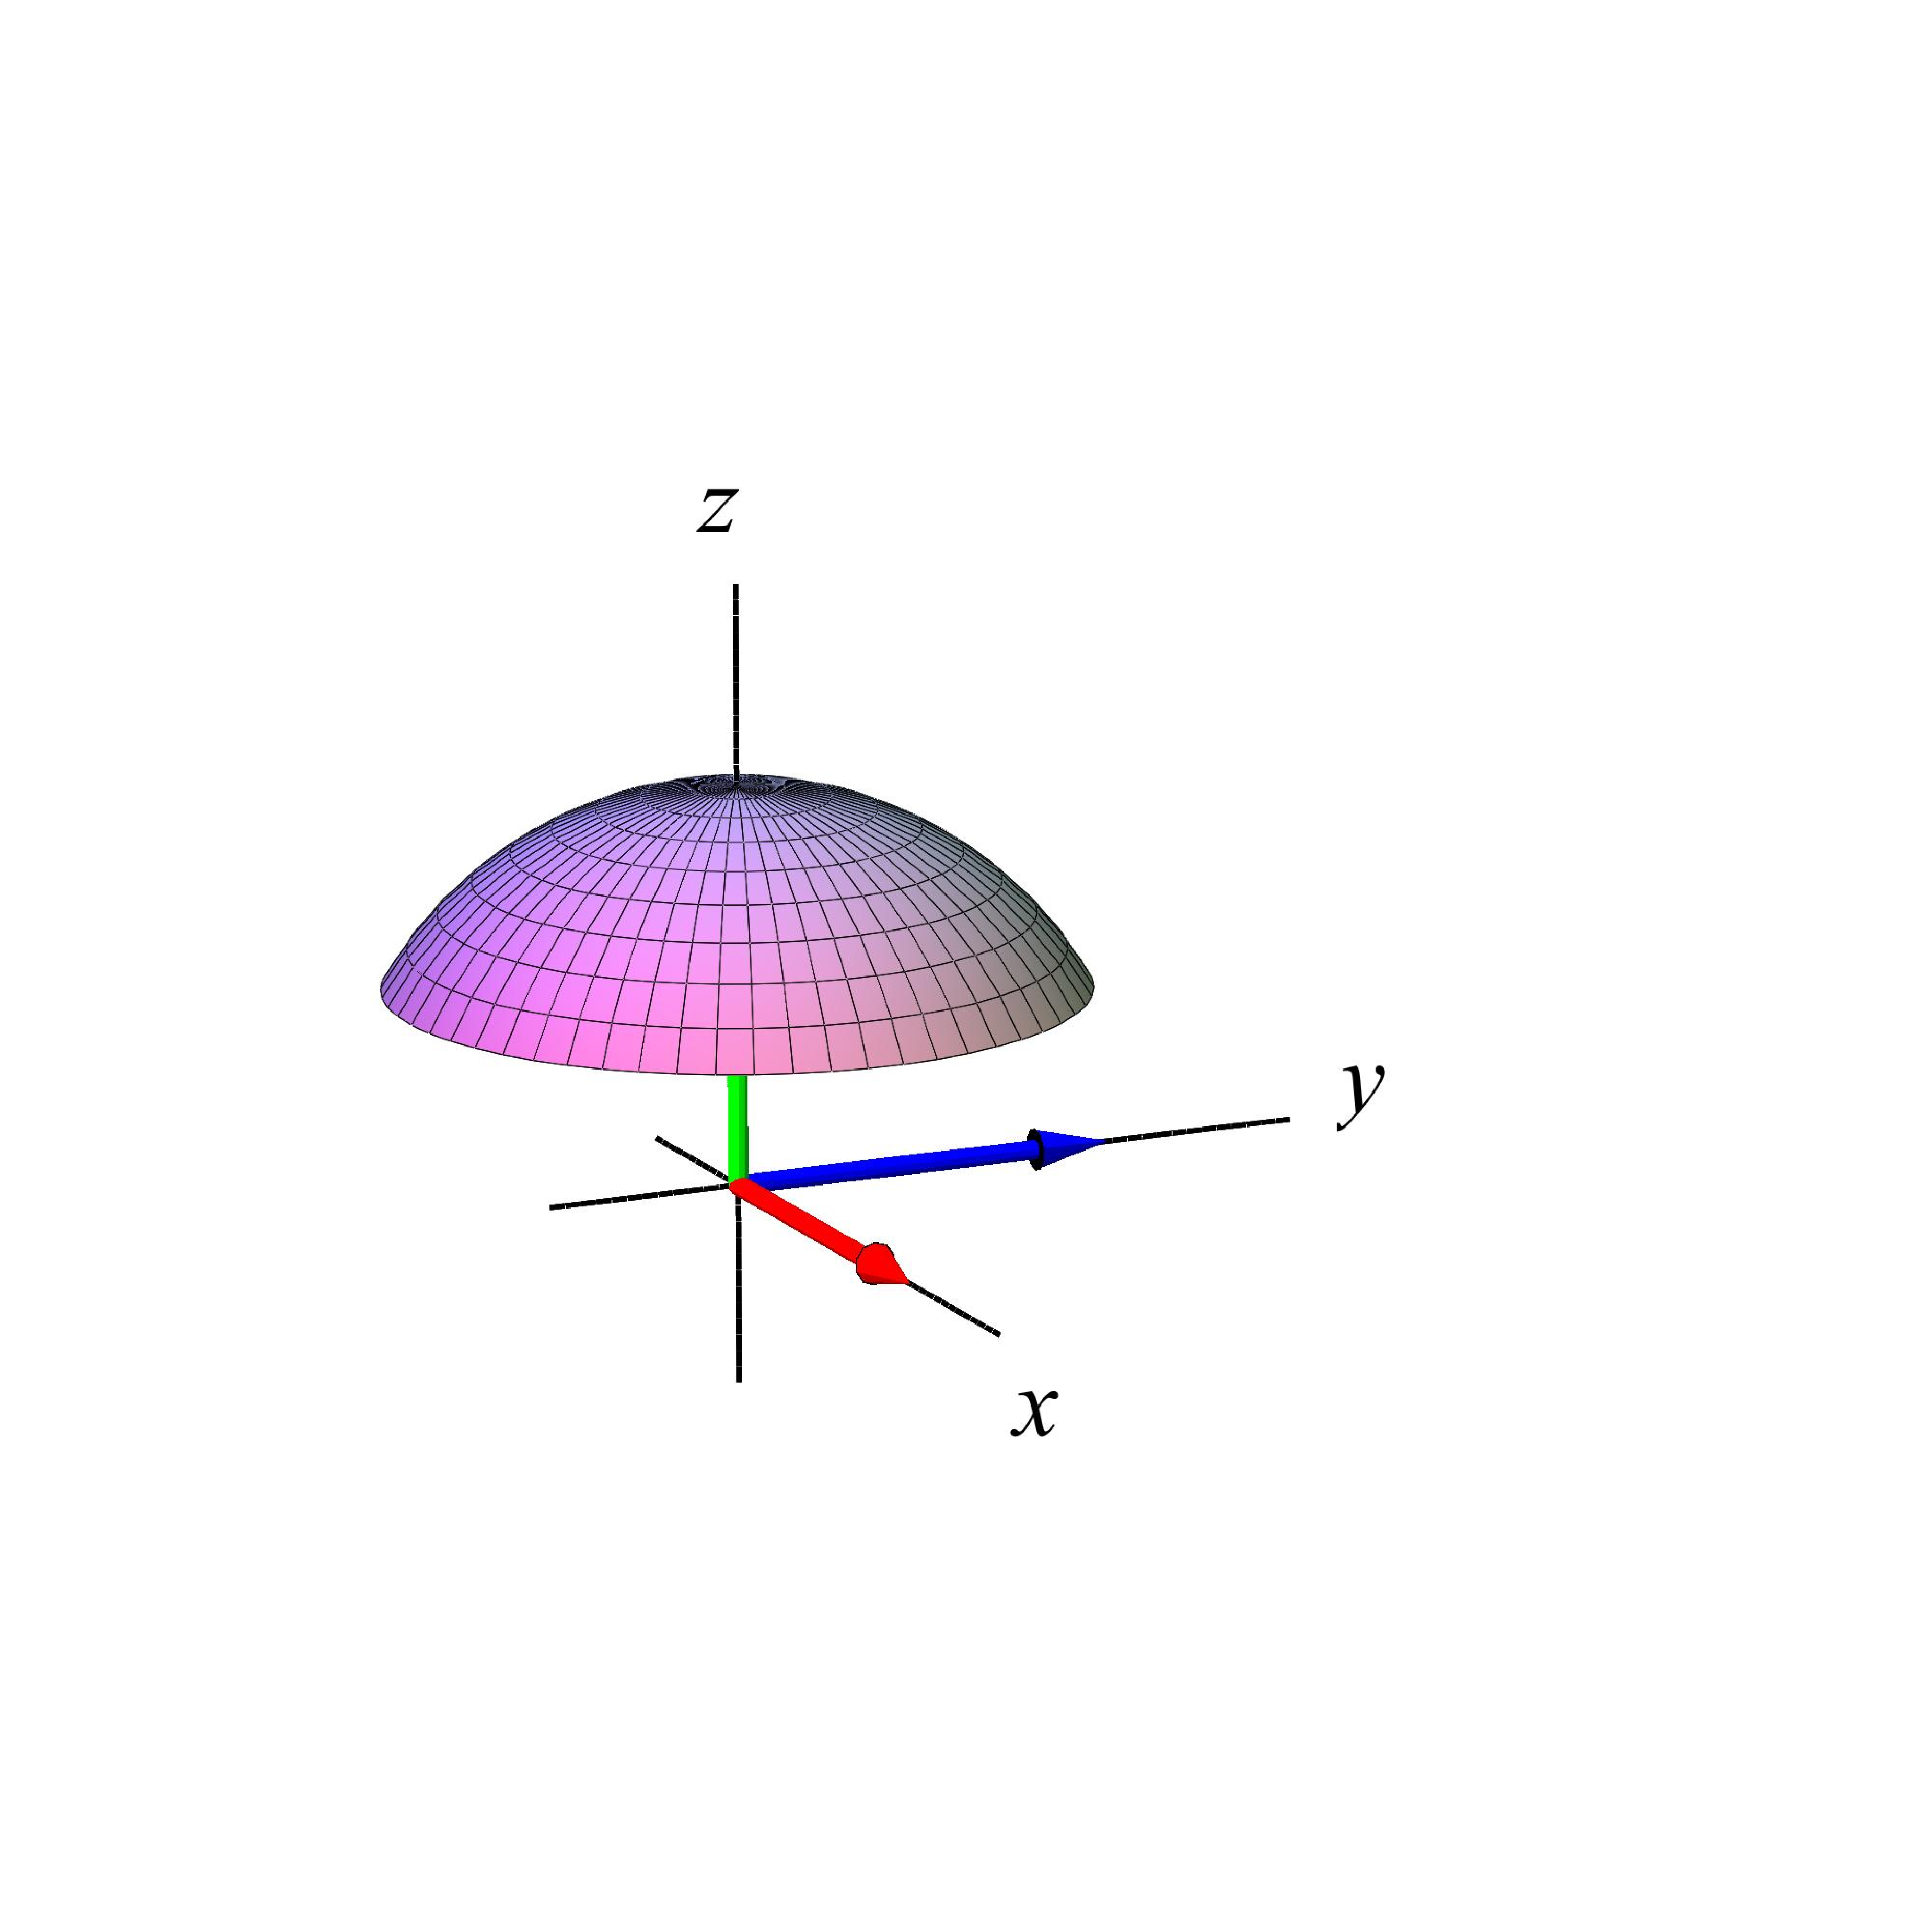
\includegraphics[width=70mm]{FIGS/plotKalotA1}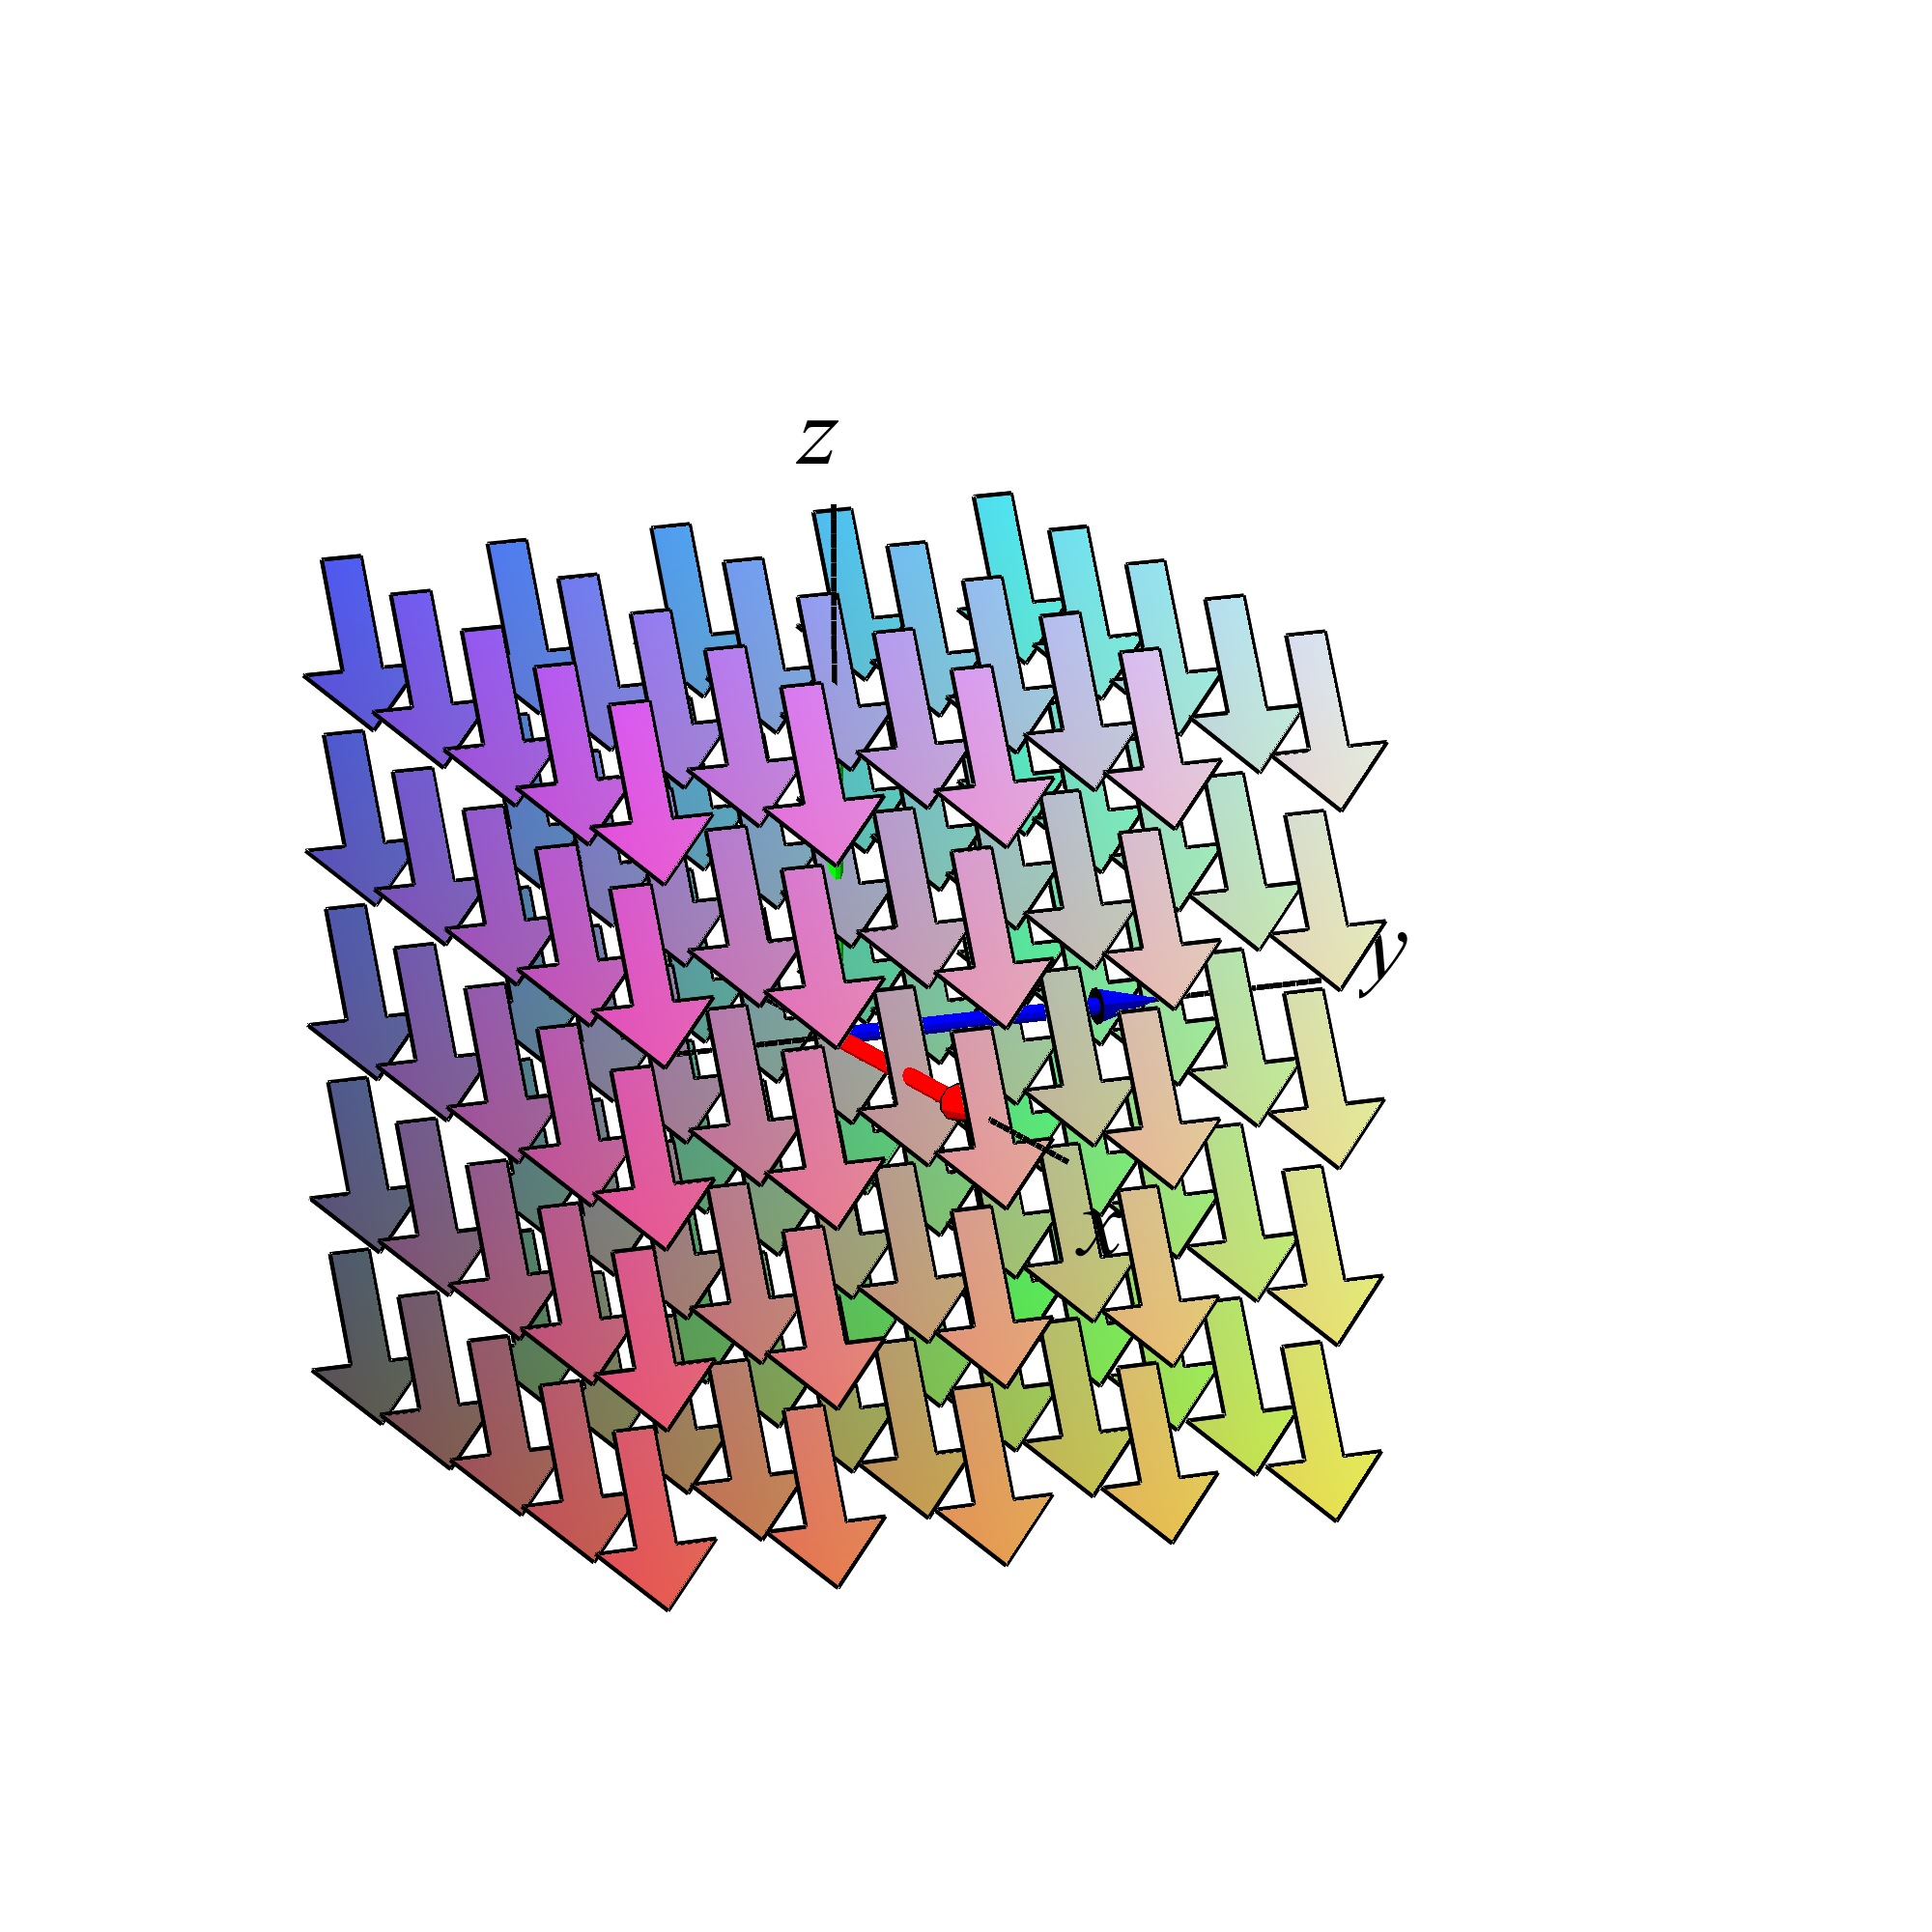
\includegraphics[width=70mm]{FIGS/plotKalotA2}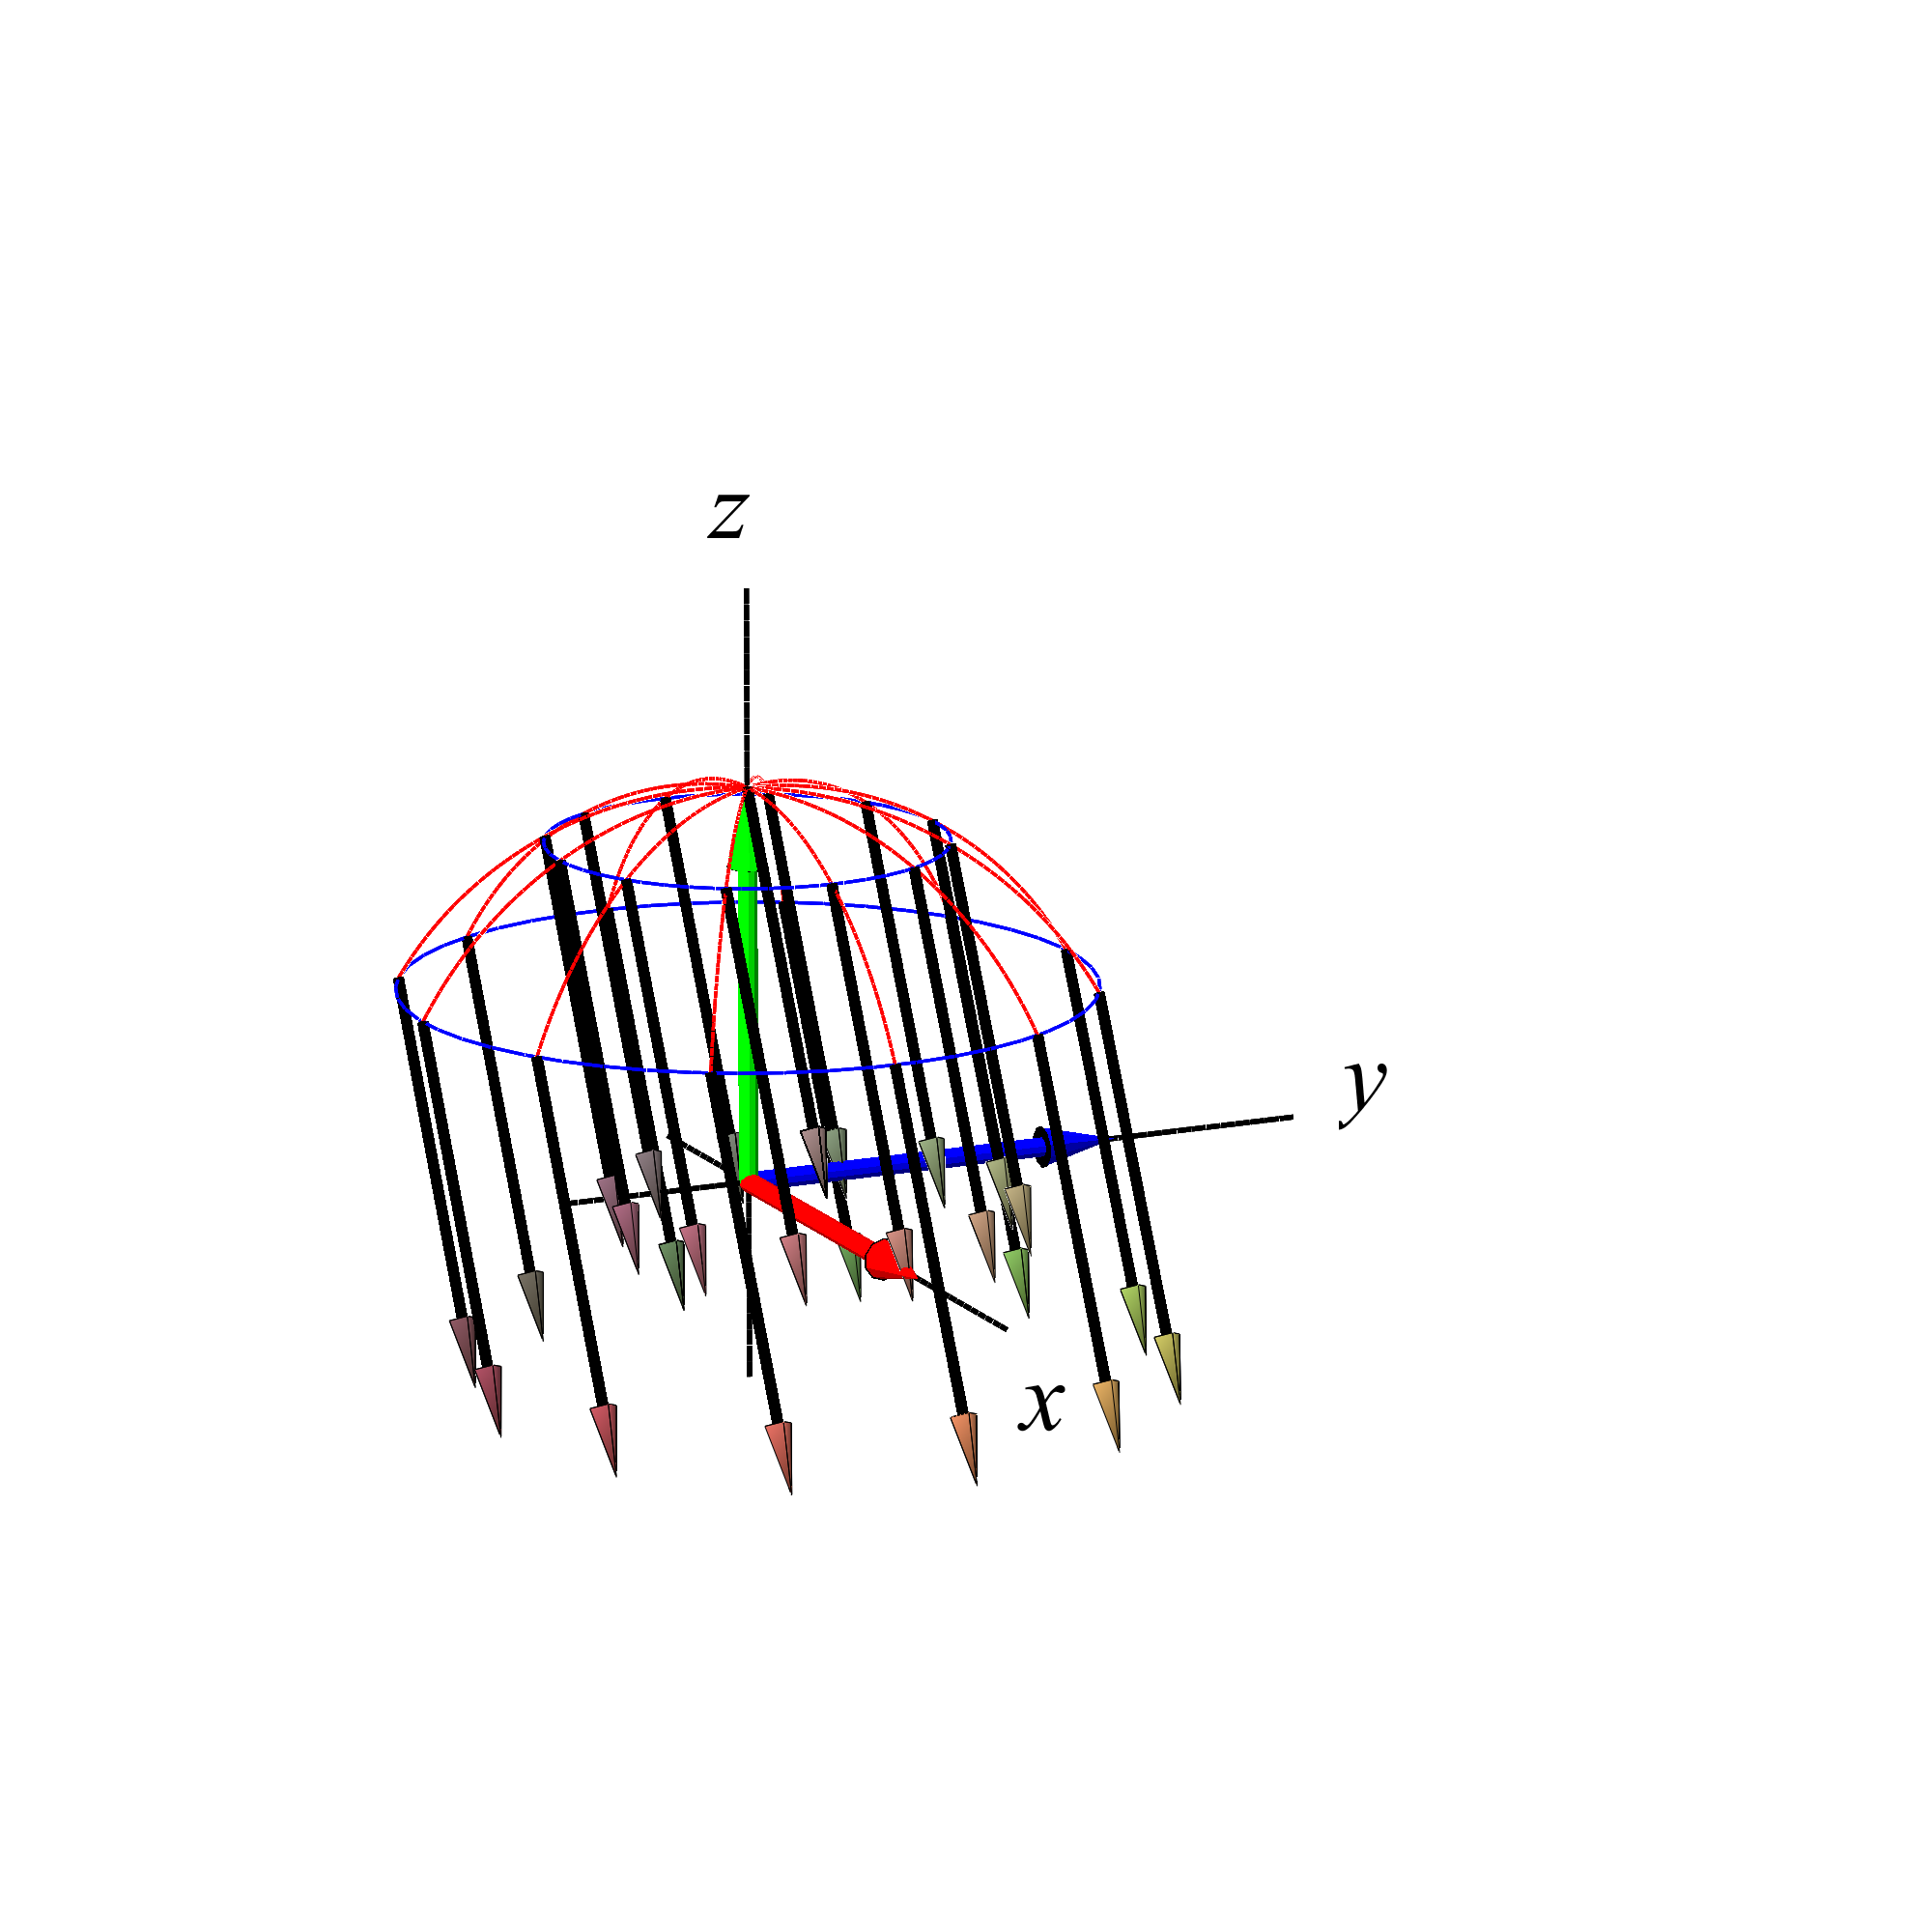
\includegraphics[width=70mm]{FIGS/plotKalotA3}}
\begin{center}
\caption{\small{Samme kalot som i figur \ref{figKalot12}. Vektorfeltet er her givet ved
${\bf V}(x,y,z) \, = \, (1, 0, -2)/\sqrt{5})$.}} \label{figKalotA12}
\end{center}
\end{figure}






%%%%%%%%%%%%%%%%%%%%%%%%%%%%%%%%%%%%%%%%%%%%
%%%%%%%%%%%%%%%%%%%%%%%%%%%%%%%%%%%%%%%%%%%%
%%%%%%%%%%%%%%%%%%%%%%%%%%%%%%%%%%%%%%%%%%%%


\begin{exercise}[En solfanger-opgave] \label{exercCyl1}
Et {solfangertag} har form som en del af en cylinder
med ligningen $x^{2} + \left(z-\frac{1}{2}\right)^{2} \, = \, 1\, $, nemlig den del, som ligger over $(x,y)-$planen og er afgrænset af $-1 \leq y \leq 1$ (vi antager som sædvanligt, at $(x,y)-$planen er vandret og at 'over' betyder $z \geq 0$), se
Figur \ref{figCylLift}.
\begin{itemize}
\item Lad os -- lidt simplificerende -- antage, at Solen stråler fra en skyfri himmel ind
på solfangertaget til et givet 'tidspunkt'
$\,t\,$ langs det enhedsvektorfelt i rummet, som
til tiden $t$ er pa\-ral\-lelt med vektoren
${\mathbf{V}}\, = \, {\mathbf{V}}(t)\, = \, (0,\,
-\cos(t),\, -\sin(t))\, $ hvor $\, t \in [0,
\pi]\, $.

\item Solen står altså op til tiden $\,t=0\,$ og sender lige på det
tidspunkt vandrette stråler parallelt med $\,y$-aksen i retningen
$\, (0, -1, 0)\, $. Midt på dagen, til tiden $\, t= \frac{\pi}{2}\,$
er strålerne lodrette og parallelle med $\,z$-aksen i retningen $\,
(0, 0, -1)\, $. Til tiden $\, t=\pi\,$ går solen ned, men lige før
det sker, sender den (næsten) vandrette stråler parallelt med
$\,y$-aksen i retningen $\, (0, 1, 0)\, $.

\item Den energi solfangeren optager pr. arealenhed og pr. tidsenhed
på et givet sted antages at være lig med
skalarproduktet ${\mathbf{V}}\cdot {\mathbf{n}}$ mellem
Solstråle-vektorfeltet ${\mathbf{V}}$ og tagfladens
{\em{indadrettede}} enhedsnormalvektor
$\,{\mathbf{n}}\,$ på stedet. Bemærk, at det
indadrettede normalfelt  $\,{\mathbf{n}}\,$ ikke
nødvendigvis er lig med $\,{\mathbf{n}}_{F}\,$, som
jo afhænger af den valgte parametrisering af
taget.
\end{itemize}

\begin{itemize}
\item Spørgsmål A:
\begin{enumerate}
\item Begrund antagelsen om, at energioptaget er
lig med skalarproduktet ${\mathbf{V}}\cdot {\mathbf{n}}$,
og bemærk, at energioptag selvsagt kun kan finde
sted hvor omtalte skalarprodukt er positiv.

\item Hvad er solfangerens energioptag pr. tidsenhed på et givet tidspunkt, $t\,$, på dagen?

\item Hvad er solfangerens totale energioptag på 'en dag'?
\end{enumerate}


\item Spørgsmål B: Antag at vi drejer det cylindriske tag $\pi/2$ mod uret (eller med) omkring $z-$aksen.
\begin{enumerate}
\item Hvad er denne drejede solfangers energioptag pr. tidsenhed på et givet tidspunkt, $t\,$, på dagen?
\item Hvad er den drejede solfangers totale energioptag på 'en dag'?
\end{enumerate}



\item Spørgsmål C:
Antag at vi drejer det oprindelige cylindriske tag fra spørgsmål A vinklen $\theta$ mod uret (eller med) omkring $z-$aksen, hvor $\theta \in [\,0, \pi/2]$.

\begin{enumerate}

\item Hvilke(t) af disse solfangertage giver det største totale energioptag pr. dag?
\end{enumerate}


\end{itemize}

\end{exercise}



\begin{figure}[h]
\centerline{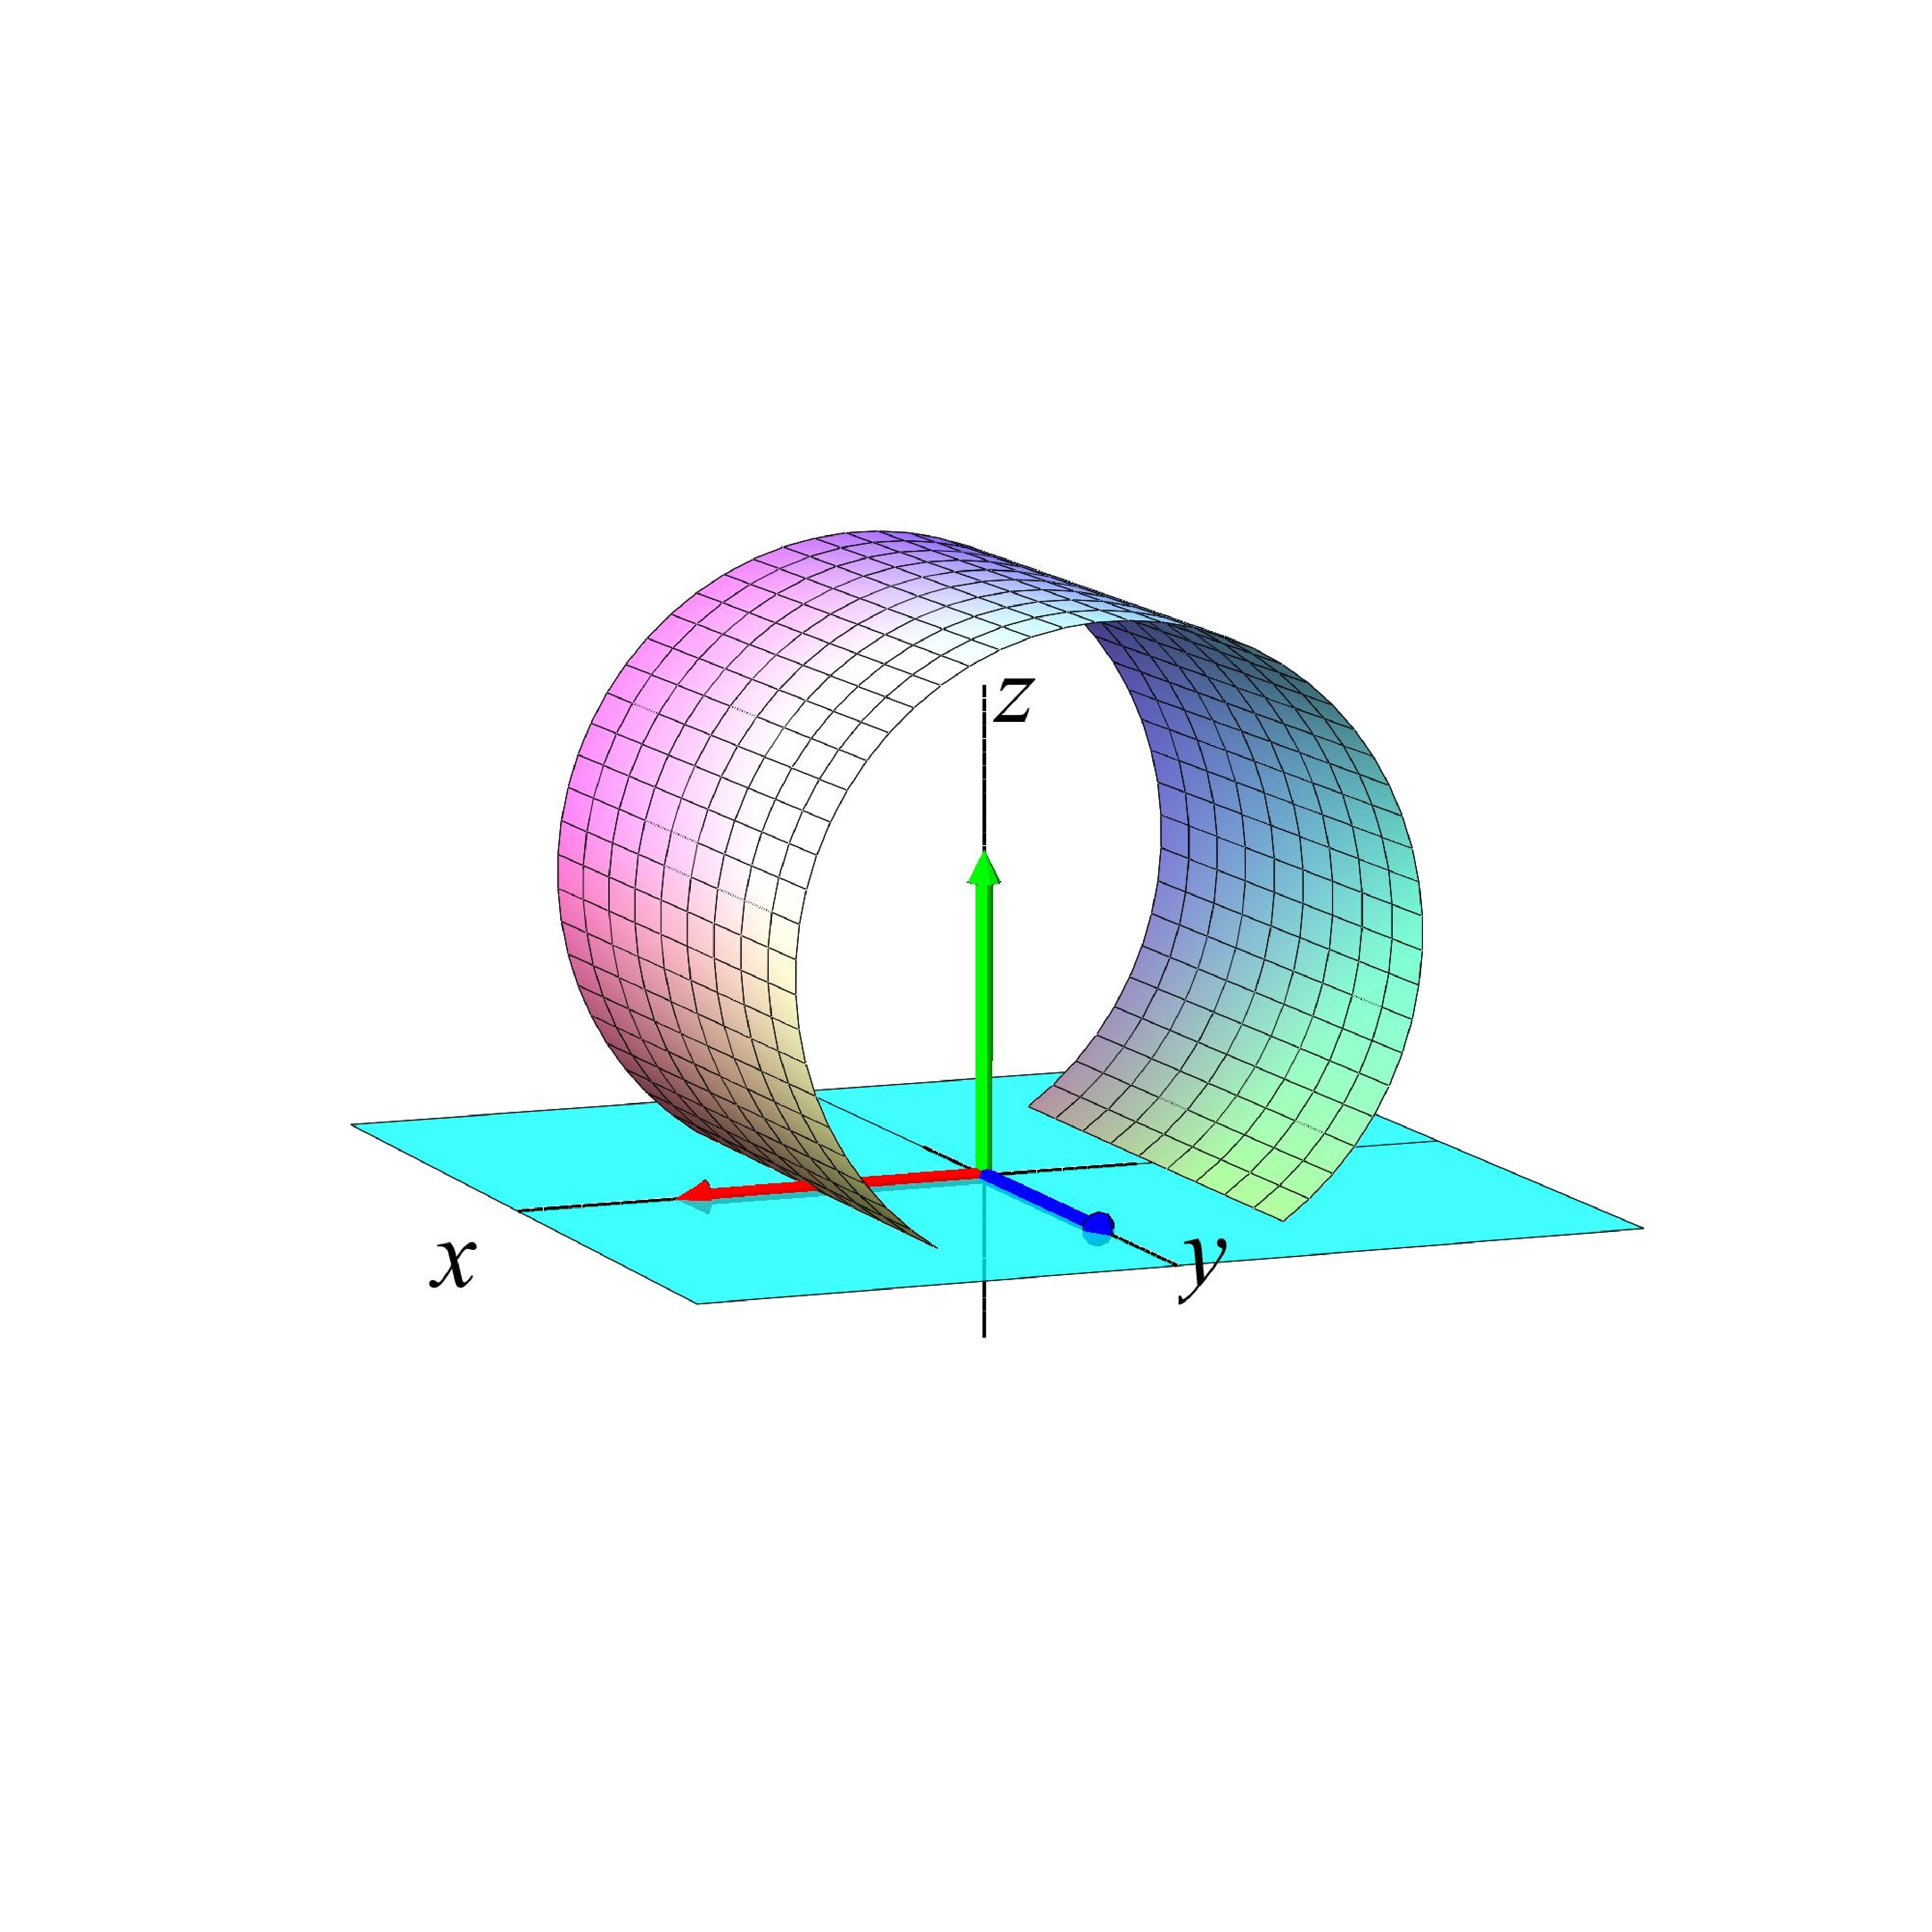
\includegraphics[width=70mm]{FIGS/plotSolCylinder}}
\begin{center}
\caption{\small{Det solfangertag der benyttes  i opgave \ref{exercCyl1}.}}
\label{figCylLift}
\end{center}
\end{figure}

%%%%%%%%%%%%%%%%%%%%%%%%%%%%%%%%%%%%%%%%%%%%%%%%%%%
%%%%%%%%%%%%%%%%%%%%%%%%%%%%%%%%%%%%%%%%%%%%%%%%%%%
%%%%%%%%%%%%%%%%%%%%%%%%%%%%%%%%%%%%%%%%%%%%%%%%%%%
%%%%%%%%%%%%%%%%%%%%%%%%%%%%%%%%%%%%%%%%%%%%%%%%%%%


\section{Motivering af fluxen via flow-ekspansion}
Integralkurverne, flowkurverne,  for et givet vektorfelt $\mathbf{V}(x,y,z)$ kan benyttes til at
'skub\-be' en given flade $F_{\mathbf{r}}$ i retning af vektorfeltet og med en lokal
fart, der er givet ved længden af vektorfeltet i ethvert punkt. Med andre ord: ethvert punkt på fladen flyder en given tid langs vektorfeltets flowkurver.

Derved gennemløber fladen -- fladen 'fejer' igennem -- et rumligt område $\Omega_{\mathbf{r}}(t)$ som til ethvert tidspunkt
$t$ (den tid vi lader fladen flyde langs vektorfeltet) har et rumfang $\Vol_{\pm}(\Omega_{\mathbf{r}}(t)) = \Vol_{\pm}(t)$.
Det rumfang er klart $0$ for $t=0$ og derefter er det lille, hvis vektorfeltet er næsten
tangentielt til fladen og stort hvis vektorfeltet er vinkelret på fladen i samme retning som standard-normalvektorfeltet på fladen.
Hvis vektorfeltet peger i modsat retning af standard-normalvektorfeltet vil vi regne de tilsvarende lokale bidrag til rumfanget negativt -- derfor betegnelsen $\Vol_{\pm}(\Omega_{\mathbf{r}}(t))$. \\

Se figurerne \ref{figSkiveFlowA}, \ref{figSkiveFlowB}, og \ref{figParabFlow} samt eksemplerne \ref{exampFlowSkive1} og \ref{exampSkiveFlowRot} hvor det illustreres hvordan Jacobifunktionen (uden numerisk tegn) kan benyttes til beregning af de lokale bidrag til rumfanget (med fortegn).\\

Der gælder følgende fundamentale sammenhæng mellem fluxen og den afledede af volumen-funktionen til tiden $t=0$:

\begin{theorem}[Fluxen som volumen-differentialkvotient ved flade-flow] \label{thmFluxVolEkspand}
Lad $\Omega_{\mathbf{r}}(t)$ betegne det rumlige område, der fejes igennem når fladestykket $F_{\bf r}$ flyder tiden $t$ med flowkurverne gennem fladens punkter. Så gælder følgende sammenhæng, hvor $\Vol_{\pm}(\Omega_{\mathbf{r}}(t))$ betegner det med fortegn beregnede
volumen af området, dvs. i forhold til den valgte standard normalvektor $\mathbf{n}_{F}(u,v)$ for $F_{\bf r}$.
\begin{equation}
\Flux({\bf V}, F_{\bf r}) = \frac{d}{dt}_{|_{t=0}}\Vol_{\pm}(\Omega_{\mathbf{r}}(t)) = \Vol'_{\pm}(0) \quad.
\end{equation}
\end{theorem}



\begin{aha}
Det er den egenskab (i sætning \ref{thmFluxVolEkspand}), der motiverer \emph{betegnelsen} flux: Lokalt er fluxen et mål for den (med fortegn regnede) volumen-vækst-rate, der øjeblikkeligt genereres ved flowet af fladen langs vektorfeltets integralkurver igennem fladens punkter. Fortegnet er positivt hvor vektorfeltet danner en spids vinkel med standard normalvektorfeltet $\mathbf{n}_{F}(u,v)$, og negativt hvor vinklen er stump. Se figurerne \ref{figParabFlow} og \ref{figSkiveFlowA}.
\end{aha}


\begin{bevis}
Vi antager som vanligt, at fladen $F_{\mathbf{r}}$ er givet ved en glat parameterfremstilling:
\begin{equation}
F_{\bf r}\quad : \quad \mathbf{r}(u,v) = (x(u,v), y(u,v), z(u,v))\quad , \quad (u,v) \in [a,b] \times [c,d] \quad .
\end{equation}
Flowkurven for $\mathbf{V}(x,y,z)$ igennem flade-punktet $\mathbf{r}(u,v)$ vil vi kalde $\tilde{\mathbf{r}}(u,v,t)$. Det område $\Omega_{F_{\mathbf{r}}}(t)$ i rummet, som fejes ud af fladen ved at den flyder med flowkurverne indtil tiden $t$ er derfor givet ved parameterfremstillingen:
\begin{equation}
\Omega_{F_{\mathbf{r}}}(t) \quad : \quad \tilde{\mathbf{r}}(u,v,w)\quad , \quad w \in [0, t] \,\, ,  \, \, u \in [a,b] \,\, ,  \, \, v \in [c, d] \quad .
\end{equation}
Til bestemmelse af rumfanget (med fortegn) af dette område benytter vi Taylor's grænseformel til første orden med udviklingspunkt $w=0$ for hver af de glatte vektorfunktioner $\tilde{\mathbf{r}}'_{u}(u,v,w)$, $\tilde{\mathbf{r}}'_{v}(u,v,w)$, og $\tilde{\mathbf{r}}'_{w}(u,v,w)$ betragtet som funktioner af $w$ for ethvert fastholdt $(u,v)$:
\begin{equation}
\begin{aligned}
\tilde{\mathbf{r}}'_{u}(u,v,w) &= \tilde{\mathbf{r}}'_{u}(u,v,0) + \bm{\varepsilon}_{(u,v)}(w)
= \mathbf{r}'_{u}(u,v) + \bm{\varepsilon}_{(u,v)}(w) \\
\tilde{\mathbf{r}}'_{v}(u,v,w) &= \tilde{\mathbf{r}}'_{v}(u,v,0) + \bm{\varepsilon}_{(u,v)}(w)
= \mathbf{r}'_{v}(u,v) + \bm{\varepsilon}_{(u,v)}(w) \\
\tilde{\mathbf{r}}'_{w}(u,v,w) &= \tilde{\mathbf{r}}'_{w}(u,v,0) + \bm{\varepsilon}_{(u,v)}(w)
= \mathbf{V}(\mathbf{r}(u,v)) + \bm{\varepsilon}_{(u,v)}(w) \quad ,
\end{aligned}
\end{equation}
sådan at Jacobifunktionen for volumen-beregningen --  med fortegn -- ser således ud:
\begin{equation}
\begin{aligned}
\Jac_{\tilde{\mathbf{r}}}(u,v,w) &= \left(\tilde{\mathbf{r}}'_{u}(u,v,w) \times \tilde{\mathbf{r}}'_{v}(u,v,w) \right) \bm{\cdot} \tilde{\mathbf{r}}'_{w}(u,v,w) \\
&= \left( \mathbf{r}'_{u}(u,v)  \times \mathbf{r}'_{v}(u,v) \right) \bm{\cdot} \mathbf{V}(\mathbf{r}(u,v)) + \varepsilon_{(u,v)}(w) \\
&= \mathbf{N}_{F}(u,v) \bm{\cdot} \mathbf{V}(\mathbf{r}(u,v)) + \varepsilon_{(u,v)}(w) \quad .
\end{aligned}
\end{equation}
Vi ser her, at når $w$ går imod $0$ opnår vi præcis det ønskede fortegn på Jacobifunktionen, som jo er det lokale bidrag (integranden) til rumfangsberegningen : Jacobifunktionen er positiv \emph{tæt ved fladen} når vektorfeltet $\mathbf{V}(\mathbf{r}(u,v))$ \emph{på fladen} peger i samme retning som standard normalvektoren $\mathbf{N}_{F}(u,v)$, og Jacobifunktionen er negativ \emph{tæt ved fladen} når vektorfeltet $\mathbf{V}(\mathbf{r}(u,v))$ \emph{på fladen} peger i modsatte retning som standard normalvektoren $\mathbf{N}_{F}(u,v)$.\\

Det med fortegn regnede rumfang $\Vol_{\pm}(\Omega_{\mathbf{r}}(t))$ er nu for tilstrækkeligt små flow-tider $t$  givet ved:
\begin{equation}
\begin{aligned}
\Vol_{\pm}(\Omega_{\mathbf{r}}(t)) &= \int_{0}^{t} \int_{c}^{d} \int_{a}^{b} \Jac_{\tilde{\mathbf{r}}}(u,v,w) \,\, du\,dv\,dw\\
&= \int_{0}^{t} \int_{c}^{d} \int_{a}^{b}\left( \mathbf{N}_{F}(u,v) \bm{\cdot} \mathbf{V}(\mathbf{r}(u,v)) + \varepsilon_{(u,v)}(w) \right)  \,\, du\,dv\,dw\\
&= \int_{0}^{t}\left( \left( \int_{c}^{d} \int_{a}^{b} \mathbf{N}_{F}(u,v) \bm{\cdot} \mathbf{V}(\mathbf{r}(u,v)) \,\, du \, dv \right) + \left( \int_{c}^{d} \int_{a}^{b} \varepsilon_{(u,v)}(w) \,\, du \, dv \right) \right) \,\, dw\\
&= \int_{0}^{t} \Flux(\mathbf{V}, F_{\mathbf{r}})\,\,dw + \int_{0}^{t} \varepsilon_{(u,v)}(w)  \,\,dw \quad,
\end{aligned}
\end{equation}
hvoraf vi aflæser:
\begin{equation}
\frac{d}{dt}\Vol_{\pm}(\Omega_{\mathbf{r}}(t)) = \Flux(\mathbf{V}, F_{\mathbf{r}}) + \varepsilon(t)
\end{equation}
og dermed
\begin{equation}
\Vol_{\pm}'(0) = \Flux(\mathbf{V}, F_{\mathbf{r}}) \quad .
\end{equation}
\end{bevis}









\begin{example}[Flow af cirkelskive ved parallelforskydning] \label{exampFlowSkive1}
Vi ser på en cirkelskive $F_{\bf r}$ i $(x,y)$-planen. Skiven har  radius $1$ og centrum i $(0,0,0)$:
\begin{equation}
F_{\bf r} \quad : \quad {\bf r}(u,v) = (u\cdot \cos(v), u\cdot \sin(v), 0) \quad , \quad  (u,v) \in [0,1]\times [-\pi, \pi] \quad .
\end{equation}
Standard normalvektoren til cirkelskiven er givet ved parametriseringen:
\begin{equation}
\begin{aligned}
\mathbf{N}_{F}(u,v) &= {\bf r}_{u}(u,v) \times {\bf r}_{v}(u,v) \\
&= ( \cos(v), \sin(v), 0) \times (-u\cdot \sin(v), u \cdot \cos(v), 0  ) \\
&= (0,0,u) \quad .
\end{aligned}
\end{equation}
Cirkelskivens enhedsnormalvektorfelt med denne parametrisering er  den konstante vektor:
\begin{equation}
{\mathbf{n}}_{F} = (0,0,1) \quad .
\end{equation}
Lad nu $\mathbf{V}(x,y,z)$ betegne vektorfeltet:
\begin{equation}
\mathbf{V}(x,y,z) = (\alpha, \beta, \gamma) \quad ,
\end{equation}
hvor $\alpha$, $\beta$, og $\gamma$ er konstanter.
Så er i dette tilfælde:
\begin{equation}
\begin{aligned}
\Flux(\mathbf{V}, F_{\bf r}) &= \int_{-\pi}^{\pi} \int_{0}^{1} \mathbf{V}(\mathbf{r}(u,v)) \bm{\cdot} \mathbf{N}_{F}(u,v) \, \, du \, dv \\
&= \int_{-\pi}^{\pi} \int_{0}^{1} (\alpha, \beta, \gamma) \bm{\cdot} ( 0,0,u) \,\, du \, dv \\
&= \int_{-\pi}^{\pi} \int_{0}^{1} u \cdot \gamma \,\, du \, dv \\
&= \gamma \cdot \pi \quad ,
\end{aligned}
\end{equation}
Bemærk, at fluxen er negativ for $\gamma <0$ og positiv for $\gamma>0$, altså i afhængighed af, om vektorfeltet peger i cirkelskivens standard normalvektor-retning eller i den modsatte retning.\\

Vi vil nu tilsvarende bestemme rumfanget af det rumlige område, som flowet af cirkelskiven 'fejer igennem' ved at følge integralkurverne, og dermed illustrere indholdet i -- og beviset for --
sætning \ref{thmFluxVolEkspand}: \\

Flowkurven $\overline{\mathbf{r}}(u,v,t)$ for $\mathbf{V}(x,y,z)$ igennem punktet $\mathbf{r}(u,v)$ er en ret linje igennem punktet, nemlig den der har den konstante tangentvektor $(\alpha, \beta, \gamma)$:
\begin{equation}
\begin{aligned}
\overline{\mathbf{r}}(u,v,t) &= \mathbf{r}(u,v) + t\cdot (\alpha, \beta, \gamma)  \\
&= (u\cdot \cos(v), u\cdot \sin(v), 0) + t\cdot (\alpha, \beta, \gamma)
\quad , \quad t\in [0, \infty[ \quad .
\end{aligned}
\end{equation}
Det ses, at
\begin{equation}
\overline{\mathbf{r}}'_{t}(u,v,t) =  (\alpha, \beta, \gamma) = \mathbf{V}(\overline{\mathbf{r}}(u,v,t)) \quad ,
\end{equation}
sådan at integralkurve-betingelsen netop er opfyldt.\\

Det rumlige område $\Omega_{F_{\mathbf{r}}}(t)$, som cirkelskiven danner ved at flyde med flowkurverne for $\mathbf{V}(x,y,z)$ indtil tiden $t$, er dermed givet ved en parameterfremstilling, som direkte aflæses af flow-kurve parameterfremstillingen igennem punkterne på fladen:
\begin{equation}
\Omega_{F_{\mathbf{r}}}(t)\quad : \quad \overline{\mathbf{r}} =  \overline{\mathbf{r}}(u,v,w) \quad , \quad w \in [0, t] \quad , \quad (u,v) \in  [0,1]\times [-\pi, \pi] \quad .
\end{equation}
Rumfanget af dette område kan findes ved hjælp af standardmetoden via Jacobifunktionen, som vi her benytter \emph{med fortegn} for at bestemme rumfanget {\emph{med  fortegn}} i forhold til normalvektoren:
\begin{equation}
\begin{aligned}
\Jac_{\overline{\mathbf{r}}}(u,v,w) &= (\overline{\mathbf{r}}_{u}(u,v,w) \times \overline{\mathbf{r}}_{v}(u,v,w)) \bm{\cdot} \overline{\mathbf{r}}_{w}(u,v,w)  \\
&= \mathbf{N}_{F}(u,v) \bm{\cdot} \overline{\mathbf{r}}_{w}(u,v,w)  \\
&= ( \cos(v), \sin(v), 0) \times (-u\cdot \sin(v), u \cdot \cos(v), 0  ) \bm{\cdot} (\alpha, \beta, \gamma) \\
&= ( 0,0,u  ) \bm{\cdot} (\alpha, \beta, \gamma)  \\
&= u \cdot \gamma    \quad ,
\end{aligned}
\end{equation}
hvor vi har benyttet, at der i dette simple konkrete tilfælde, hvor vektorfeltet paralleltransporterer cirkelskiven i vektorfeltets retning gælder: $(\overline{\mathbf{r}}_{u}(u,v,w) \times \overline{\mathbf{r}}_{v}(u,v,w))= \mathbf{N}_{F}(u,v)$ som er uafhængig af $w$.
Rumfanget {\emph{med fortegn}} af $\Omega_{F_{\mathbf{r}}}(t)$ i forhold til cirkelskivens normalvektorfelt $(0,0,1)$ er derfor
\begin{equation}
\Vol_{\pm}(t) = \int_{0}^{t}\int_{-\pi}^{\pi}\int_{0}^{1} u \cdot \gamma \, du\, dv\, dw  =   t \cdot \gamma \cdot \pi \quad.
\end{equation}
Heraf får vi
\begin{equation}
\Vol_{\pm}'(0) = \gamma \cdot \pi \quad ,
\end{equation}
altså  den samme værdi som den ovenfor fundne $\Flux(\mathbf{V}, F_{\bf r})$. Vi har dermed verificeret sætningen \ref{thmFluxVolEkspand}.\\

Hvis vektorfeltet $(\alpha, \beta, \gamma)$ er i samme retning som standard normalen  til fladen (dvs. hvis  $\gamma >0$), så er både
fluxen, rumfanget  $\Vol_{\pm}(t)$, og volumen-differentialkvotienten $\Vol_{\pm}'(0)$ positiv; hvis vektorfeltet $(\alpha, \beta, \gamma)$ er i modsatte retning i forhold til standard normalen (dvs. hvis  $\gamma <0$), så er både
fluxen, rumfanget (med fortegn) $\Vol_{\pm}(t)$, og  volumen-differentialkvotienten $\Vol_{\pm}'(0)$ negativ.
\end{example}


\begin{figure}[ht]
\centerline{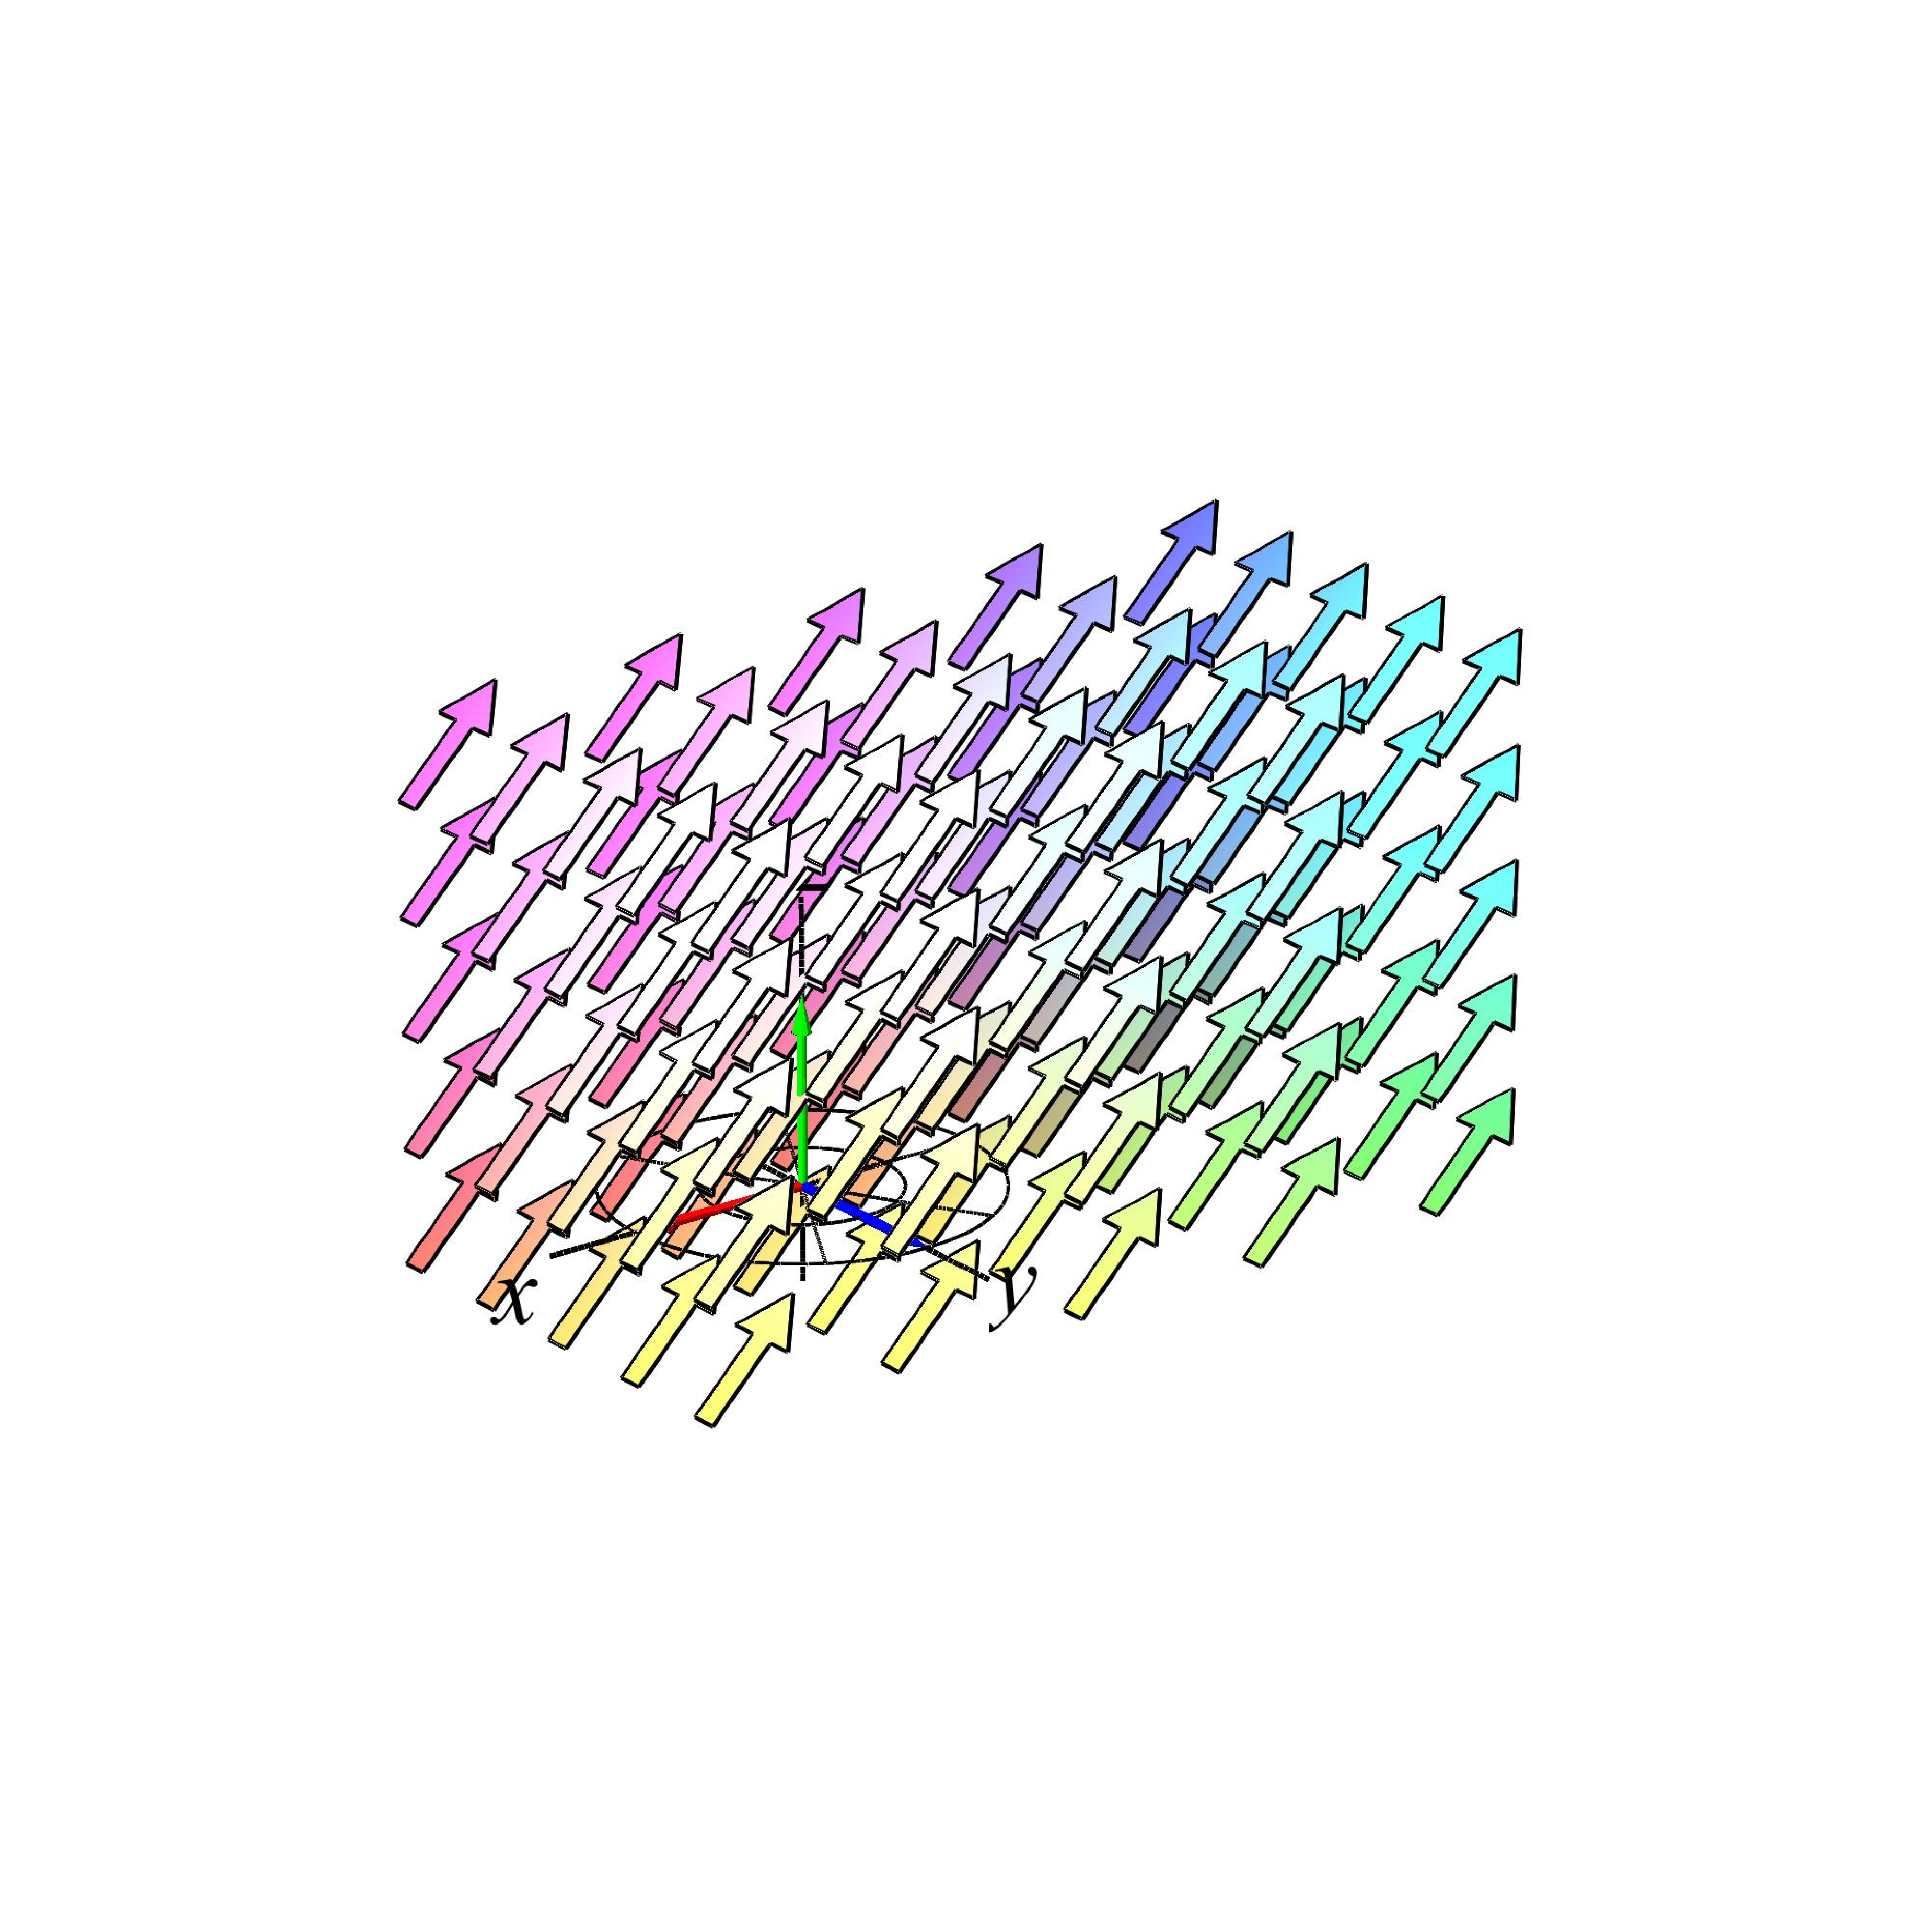
\includegraphics[width=70mm]{FIGS/plotSkiveFlowA1}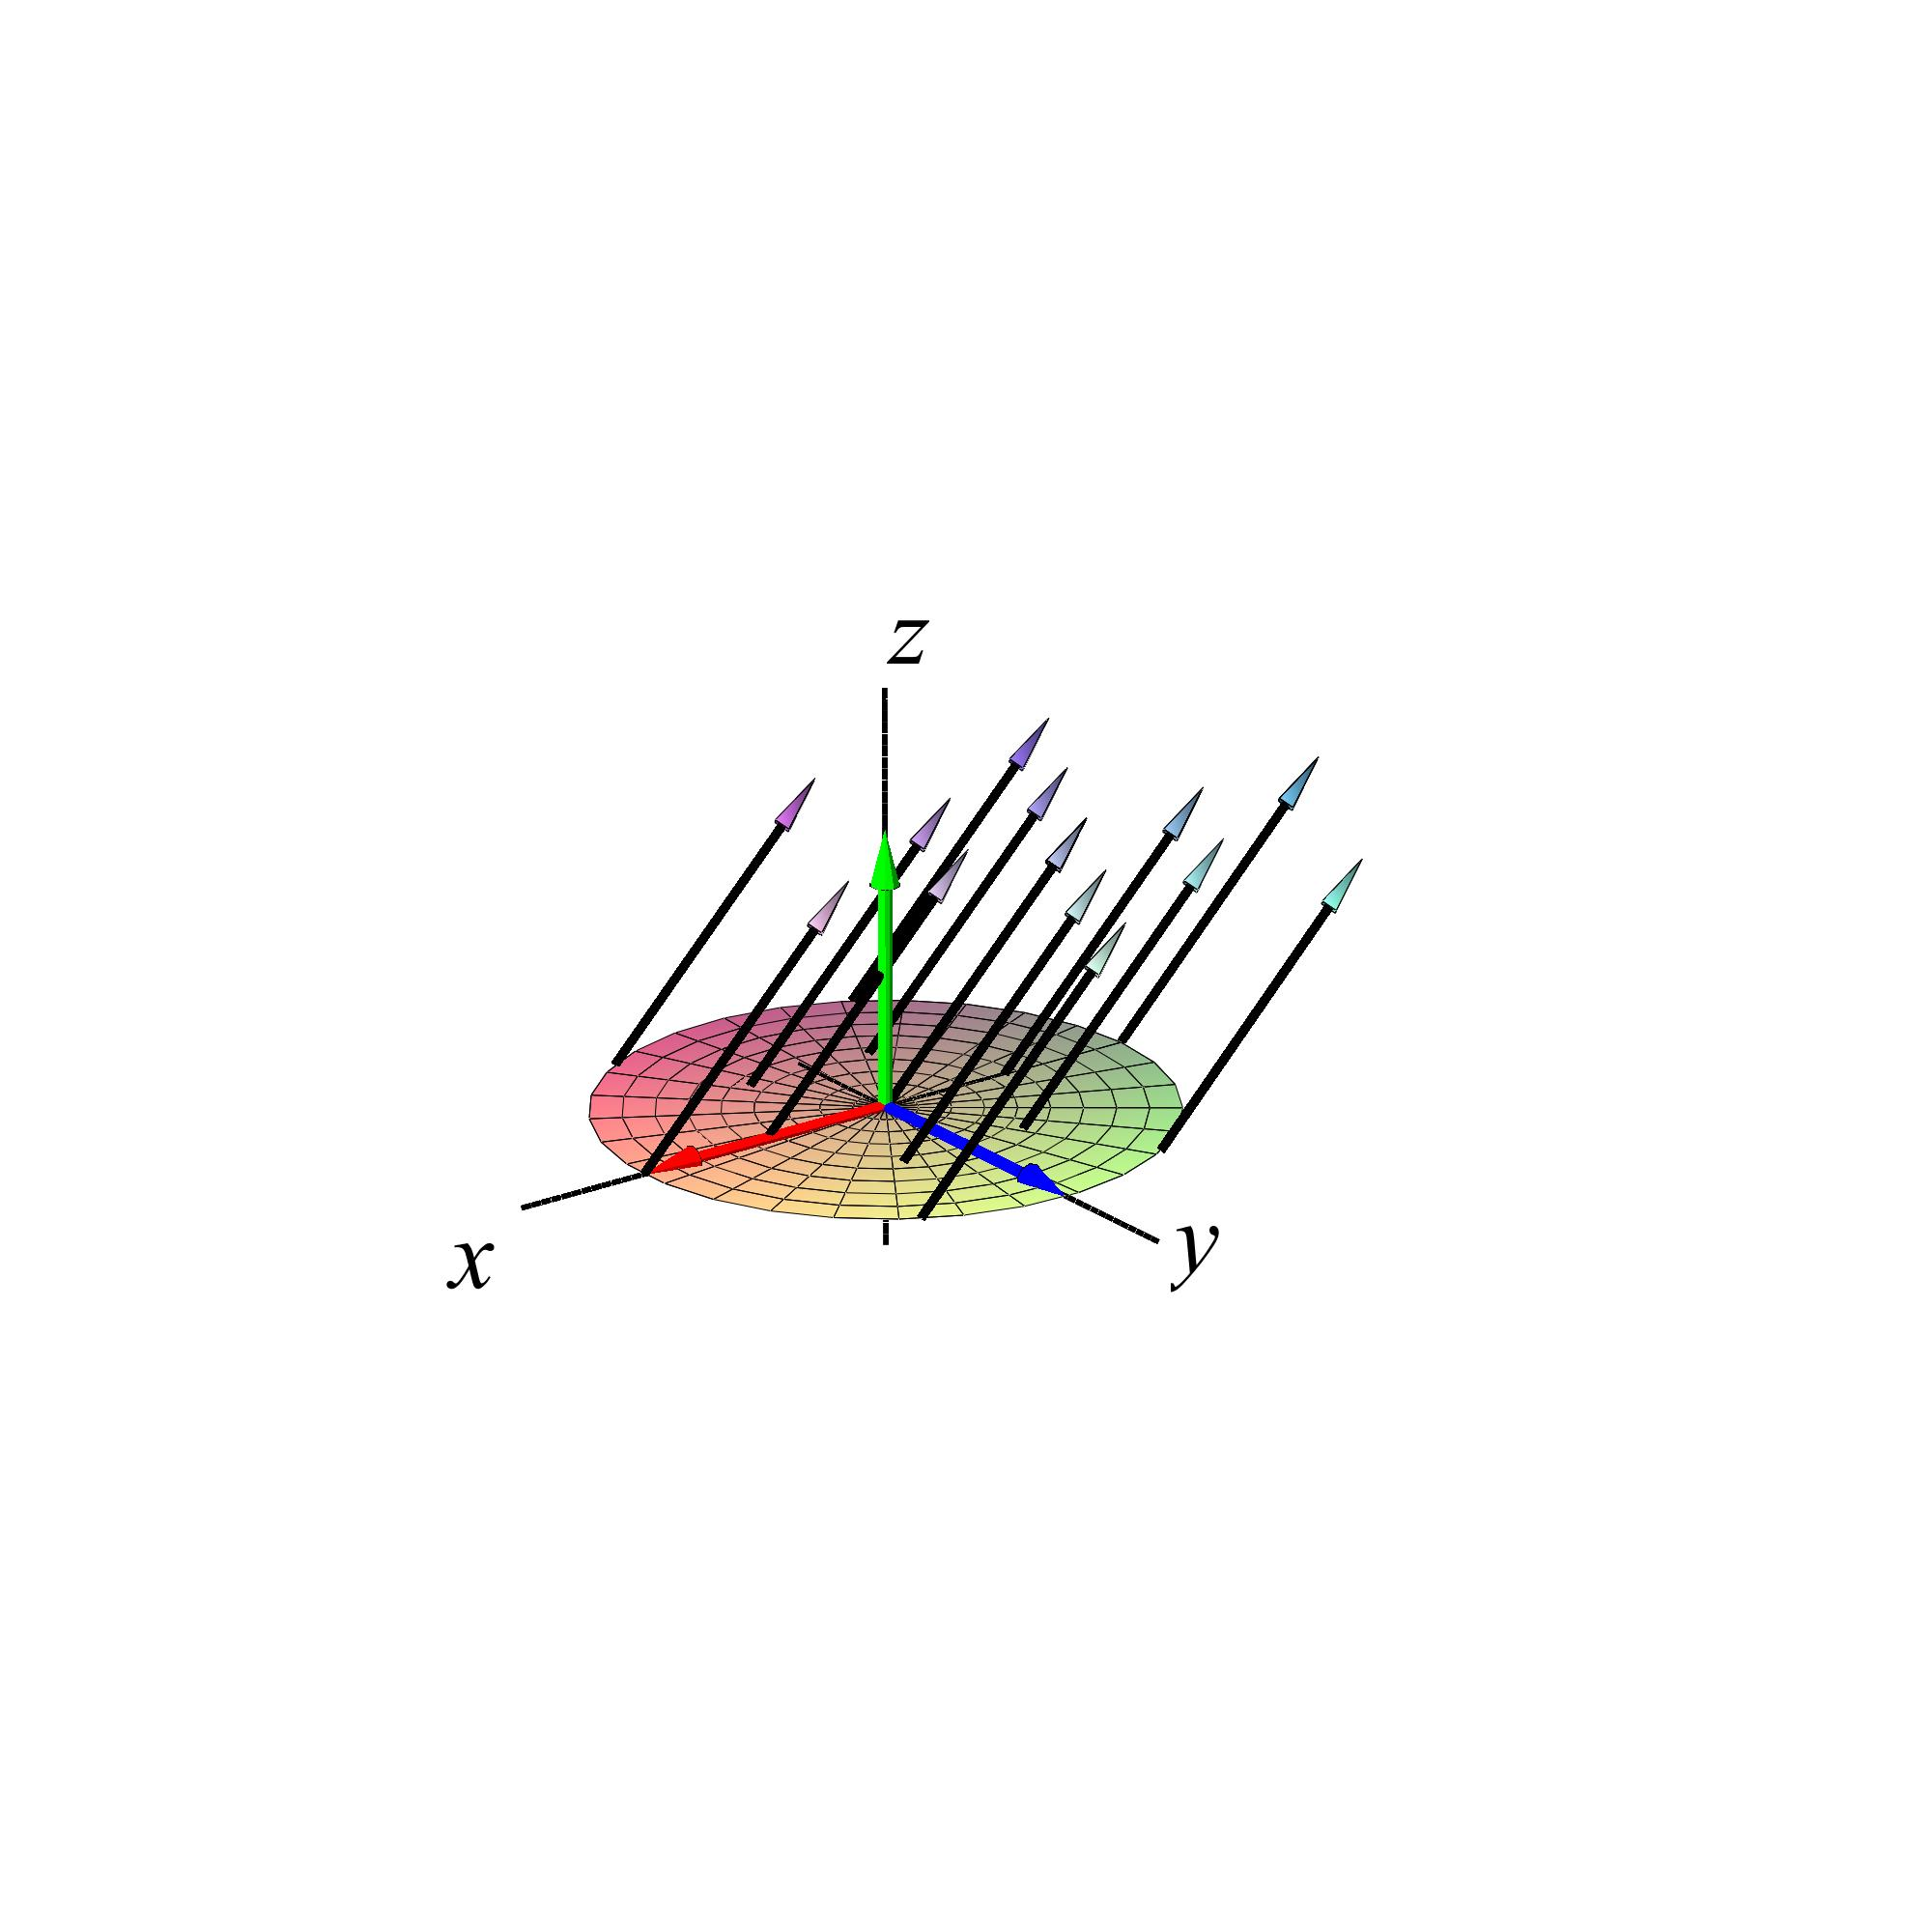
\includegraphics[width=70mm]{FIGS/plotSkiveFlowA3}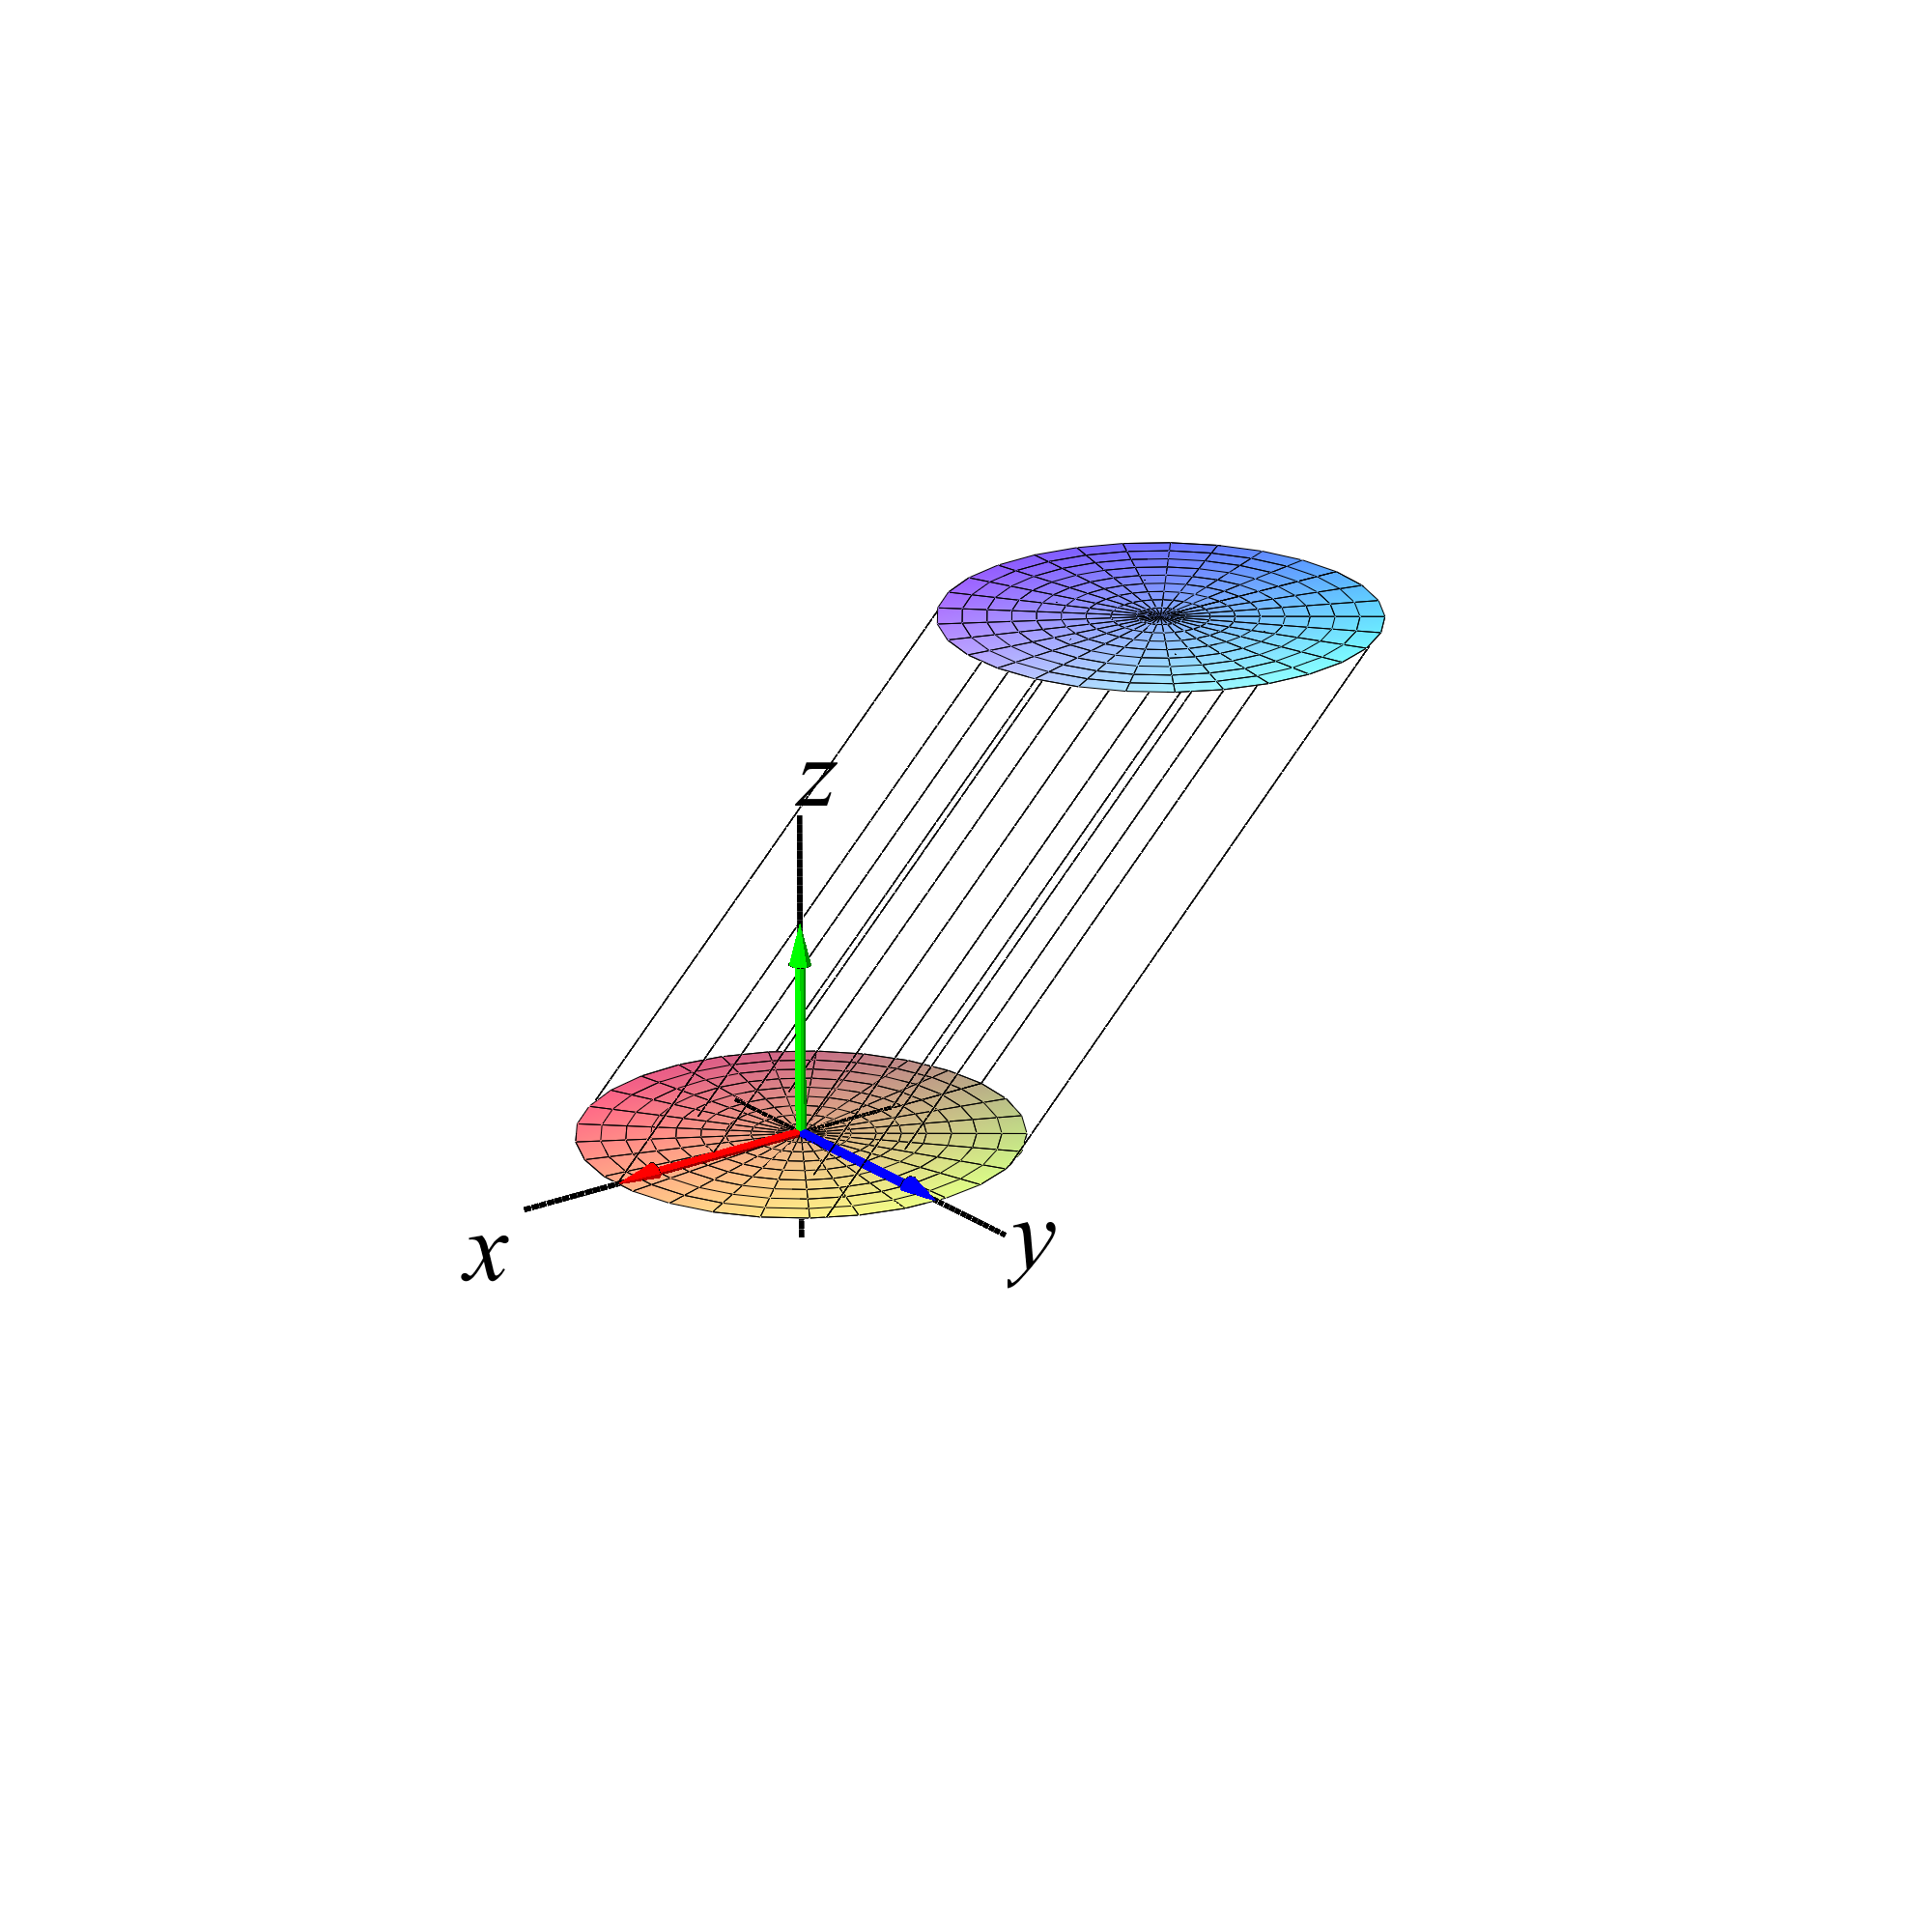
\includegraphics[width=70mm]{FIGS/plotSkiveFlowA2}}
\begin{center}
\caption{\small{Et simpelt, konstant vektorfelt, og tilsvarende kort-tids flow af en cirkelskive. I forhold til cirkelskivenormalen $(0,0,1)$ er fluxen og volumen-tilvæksten positiv. }} \label{figSkiveFlowA}
\end{center}
\end{figure}


\begin{figure}[ht]
\centerline{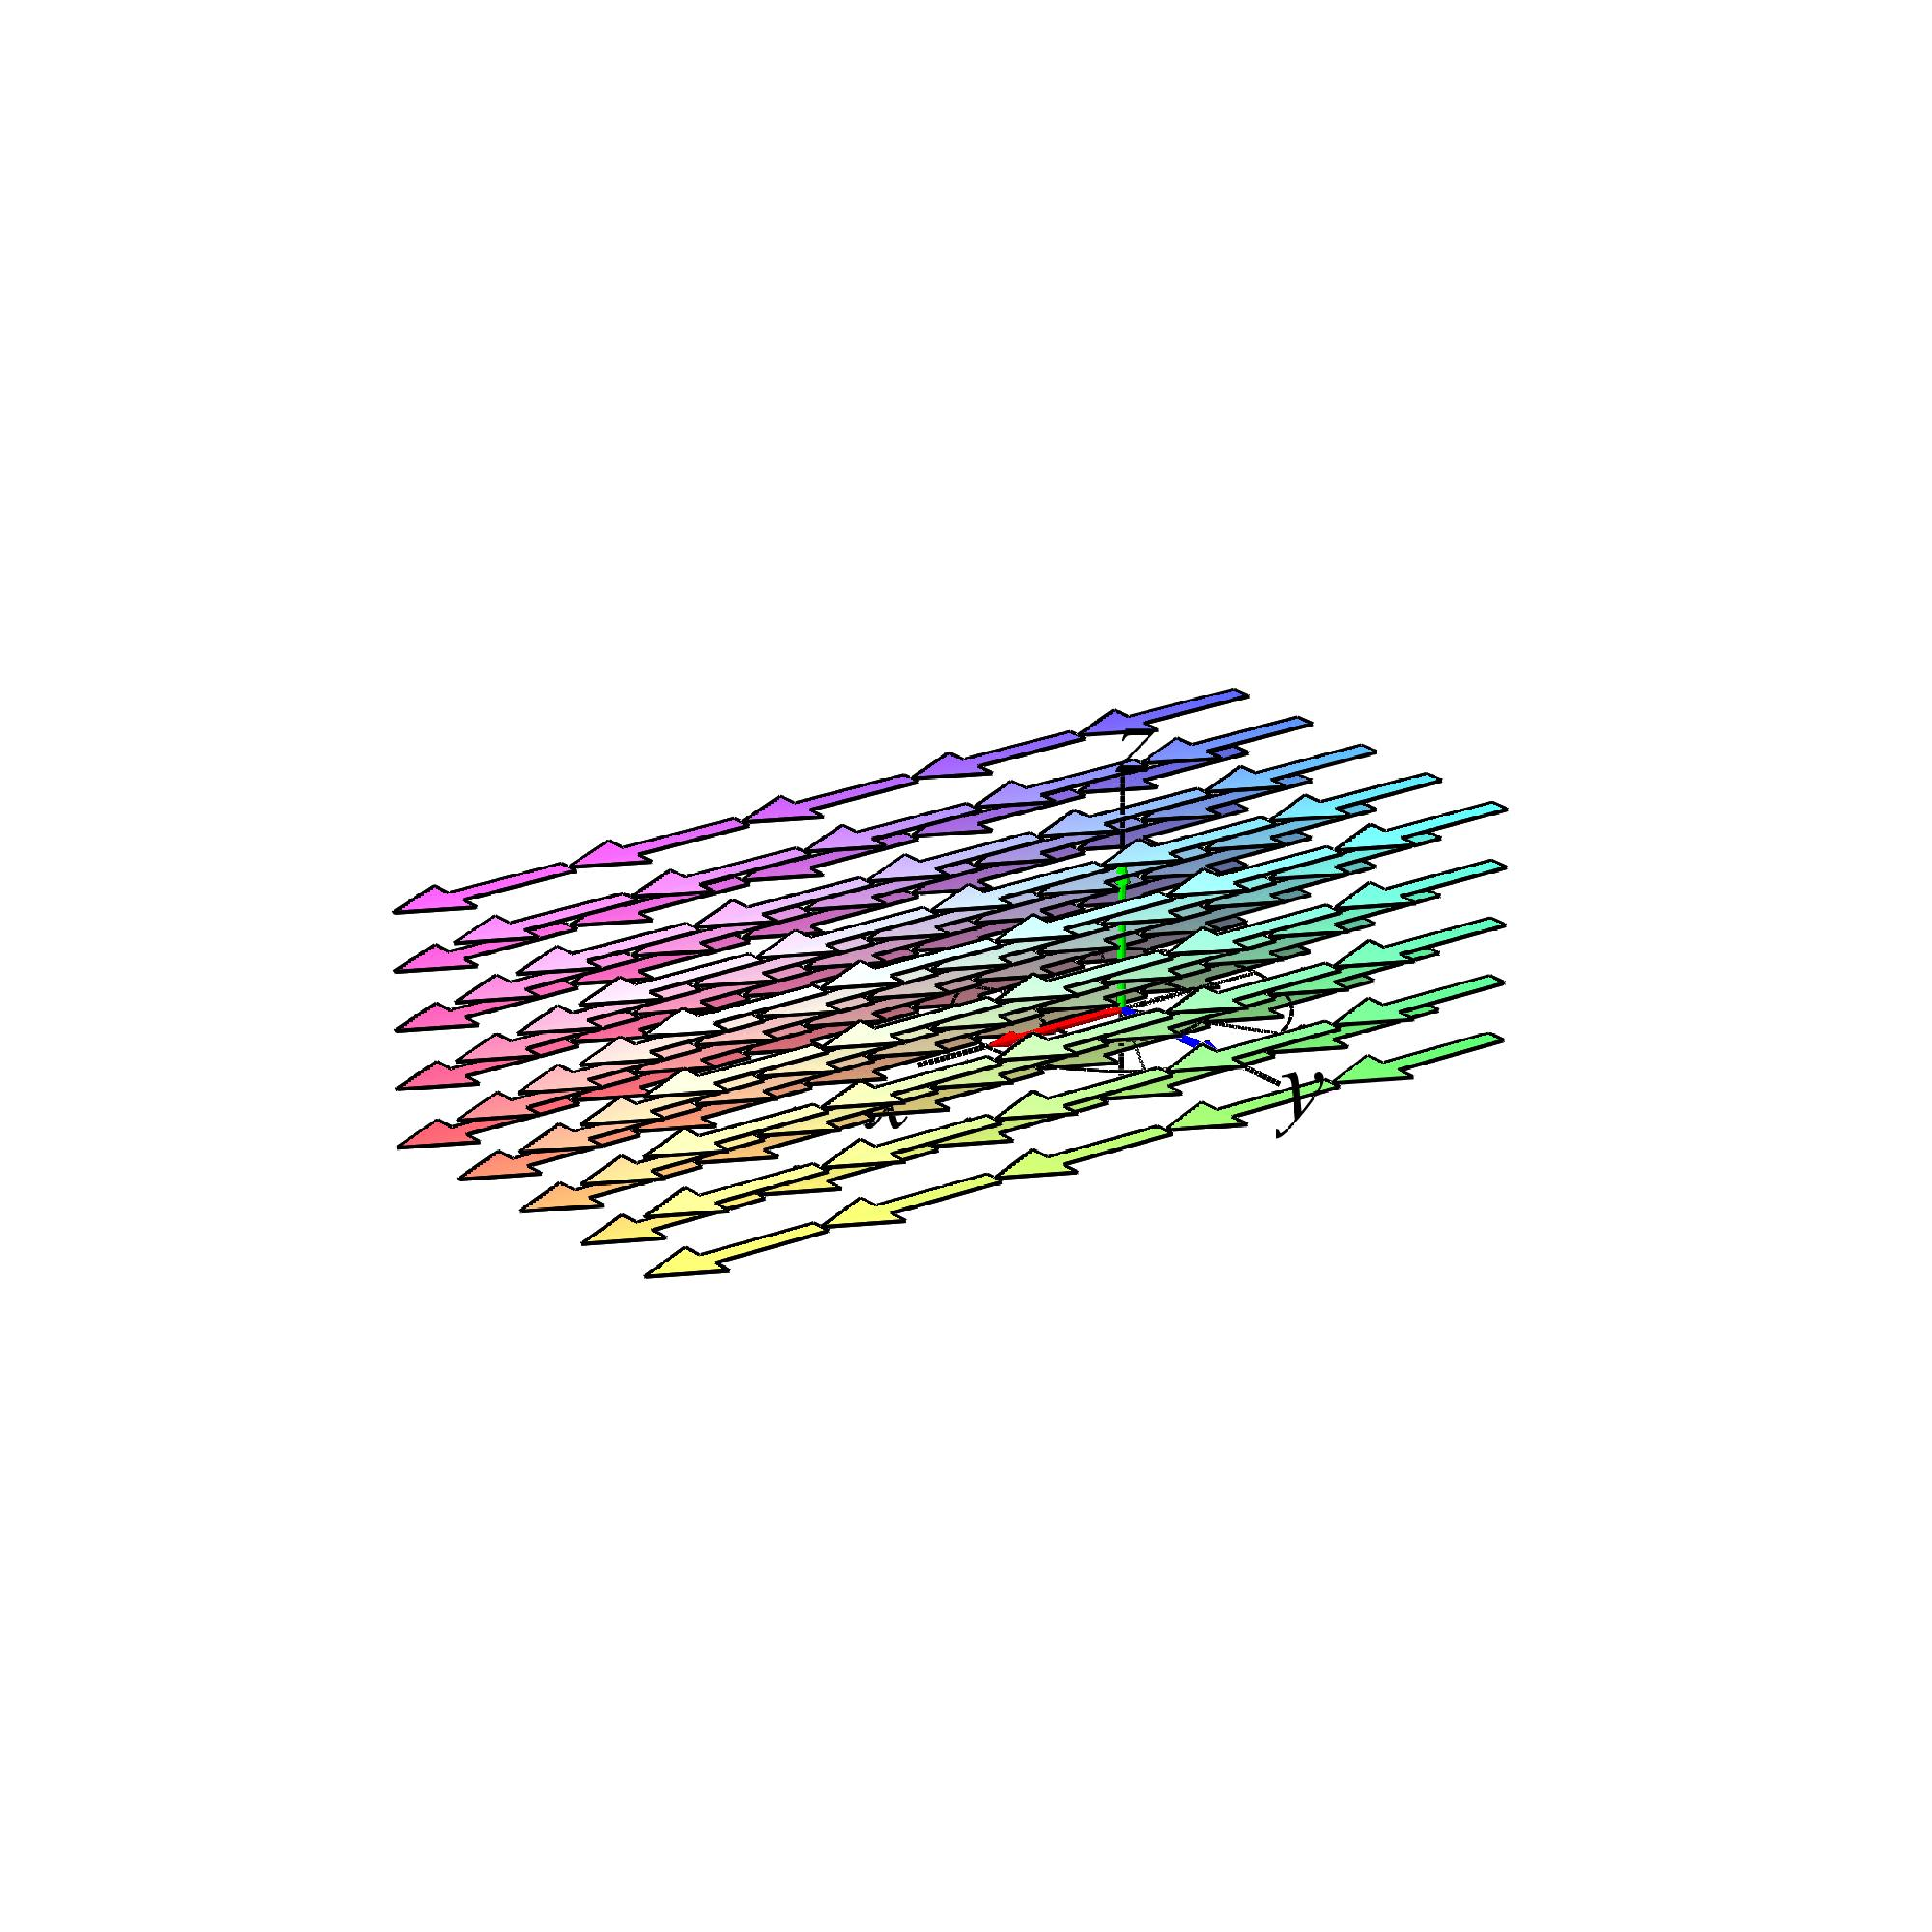
\includegraphics[width=70mm]{FIGS/plotSkiveFlowB1}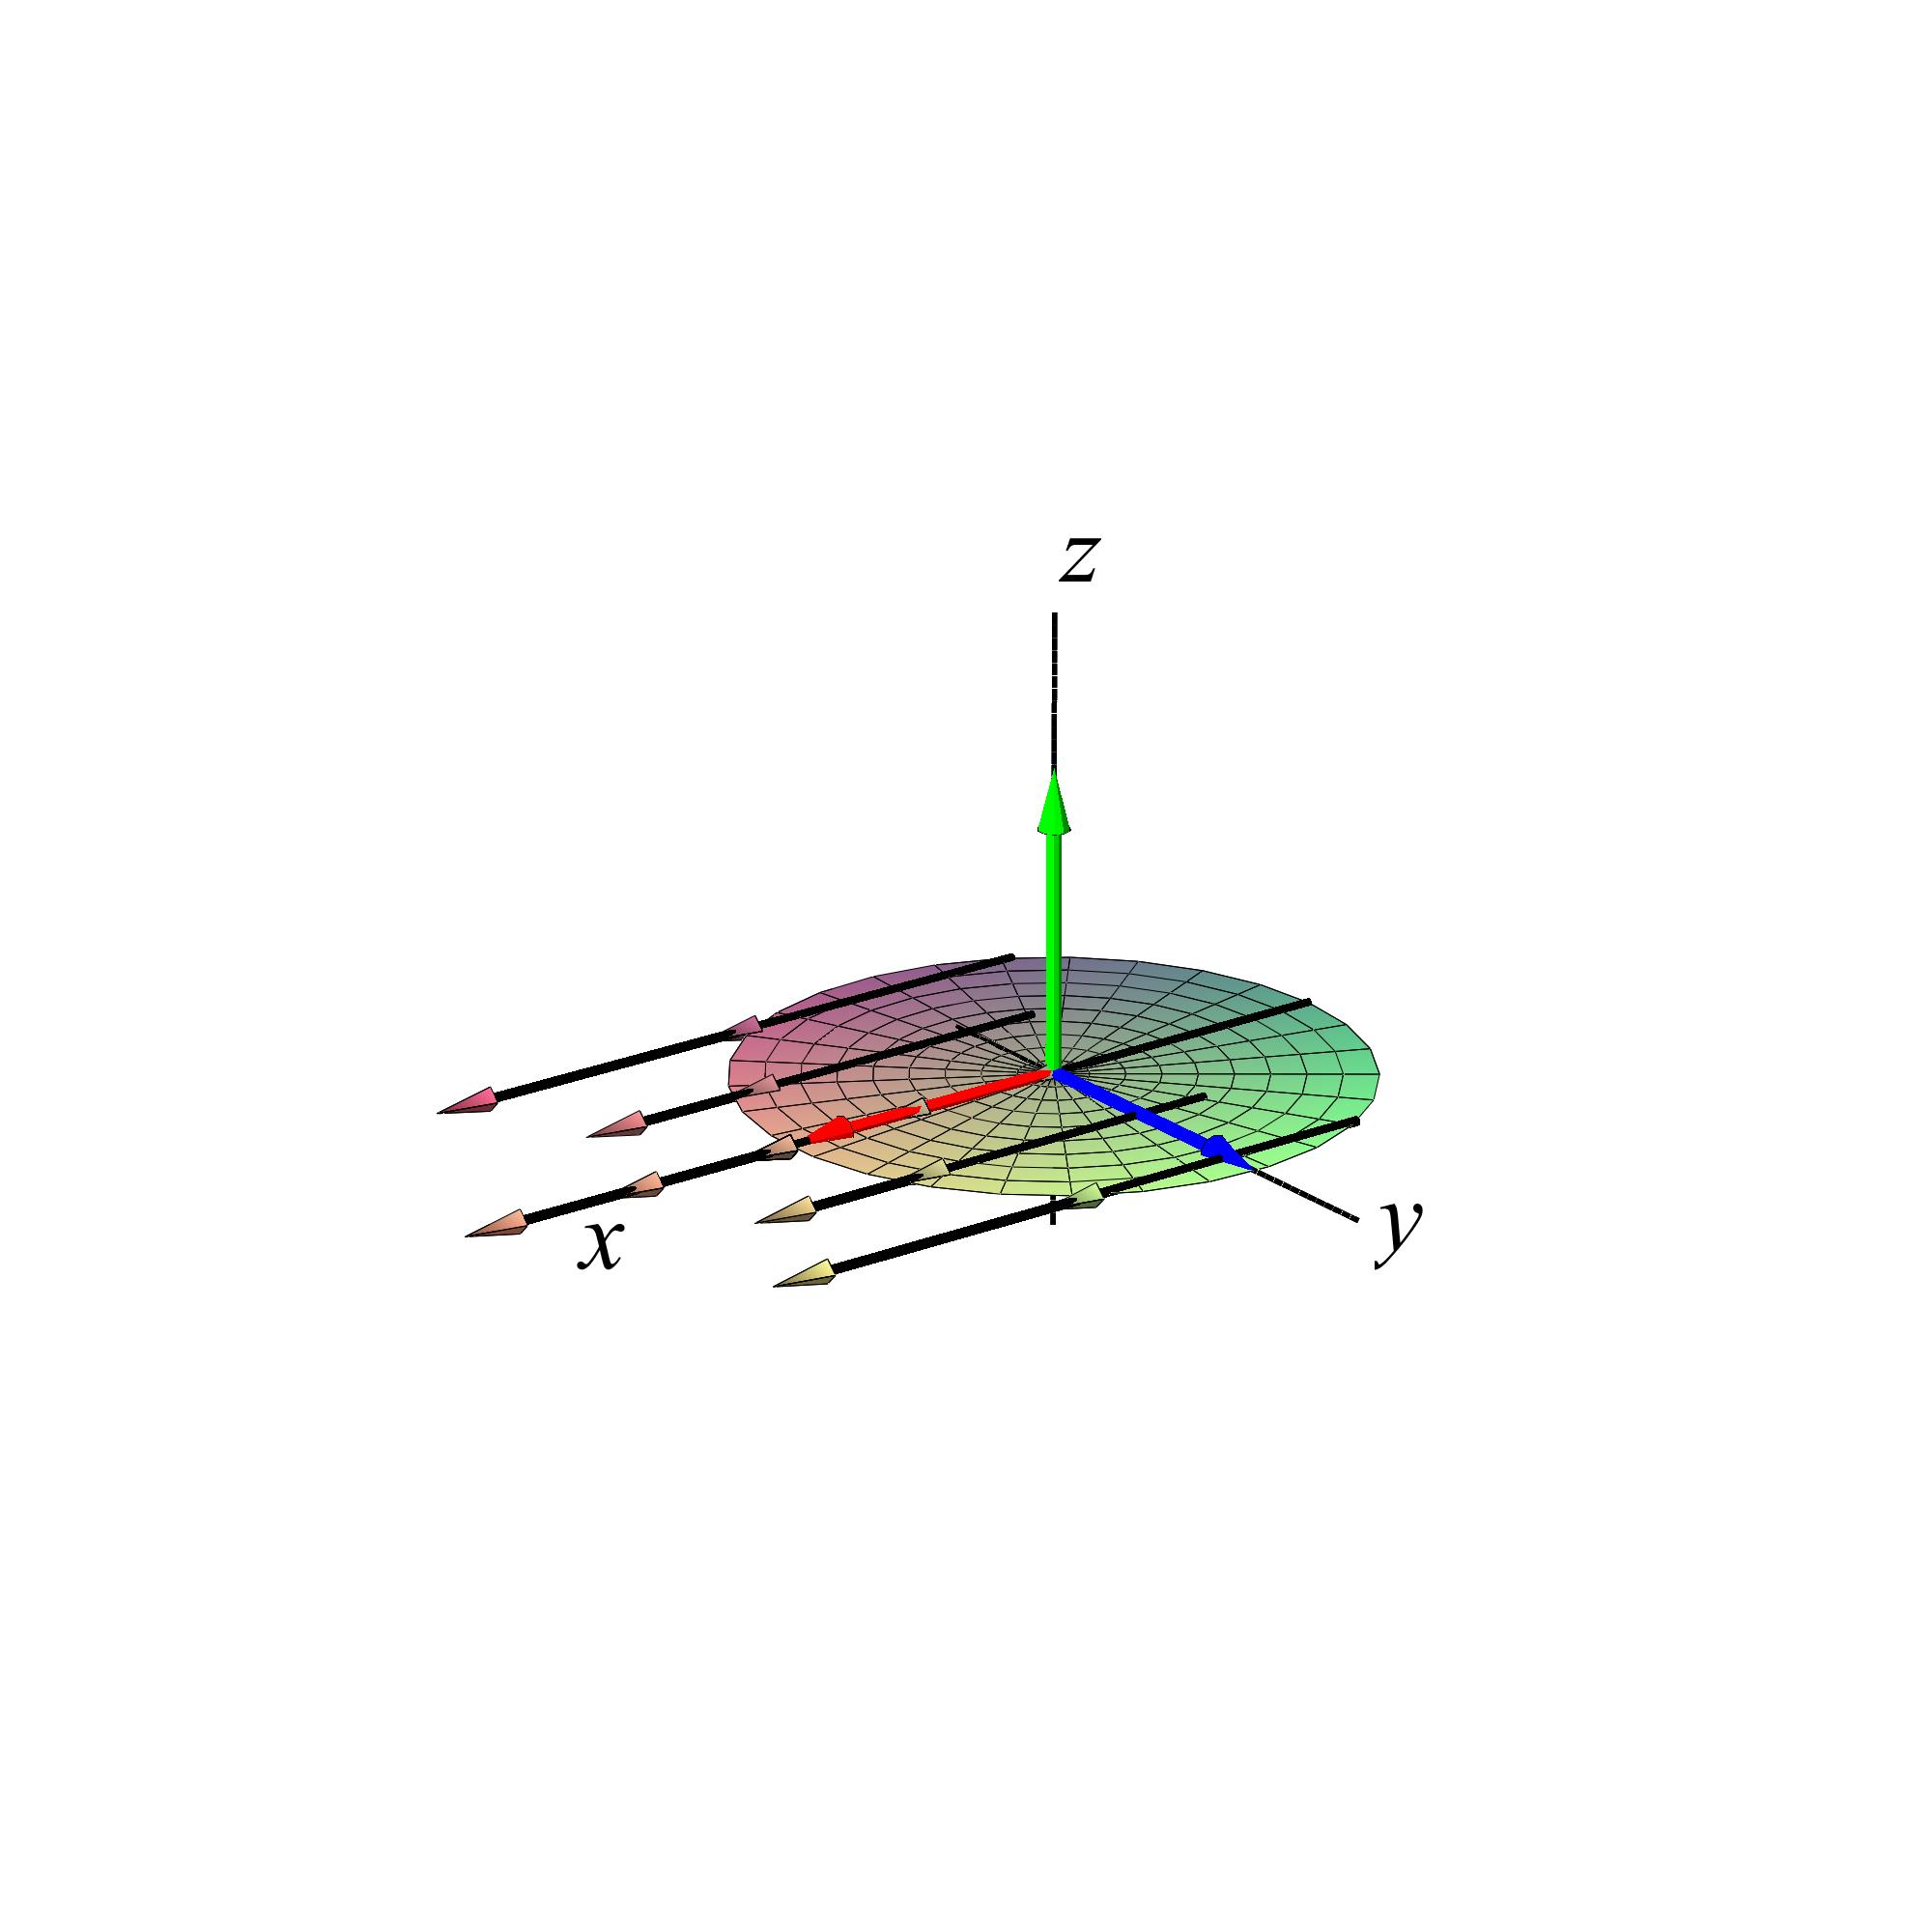
\includegraphics[width=70mm]{FIGS/plotSkiveFlowB3}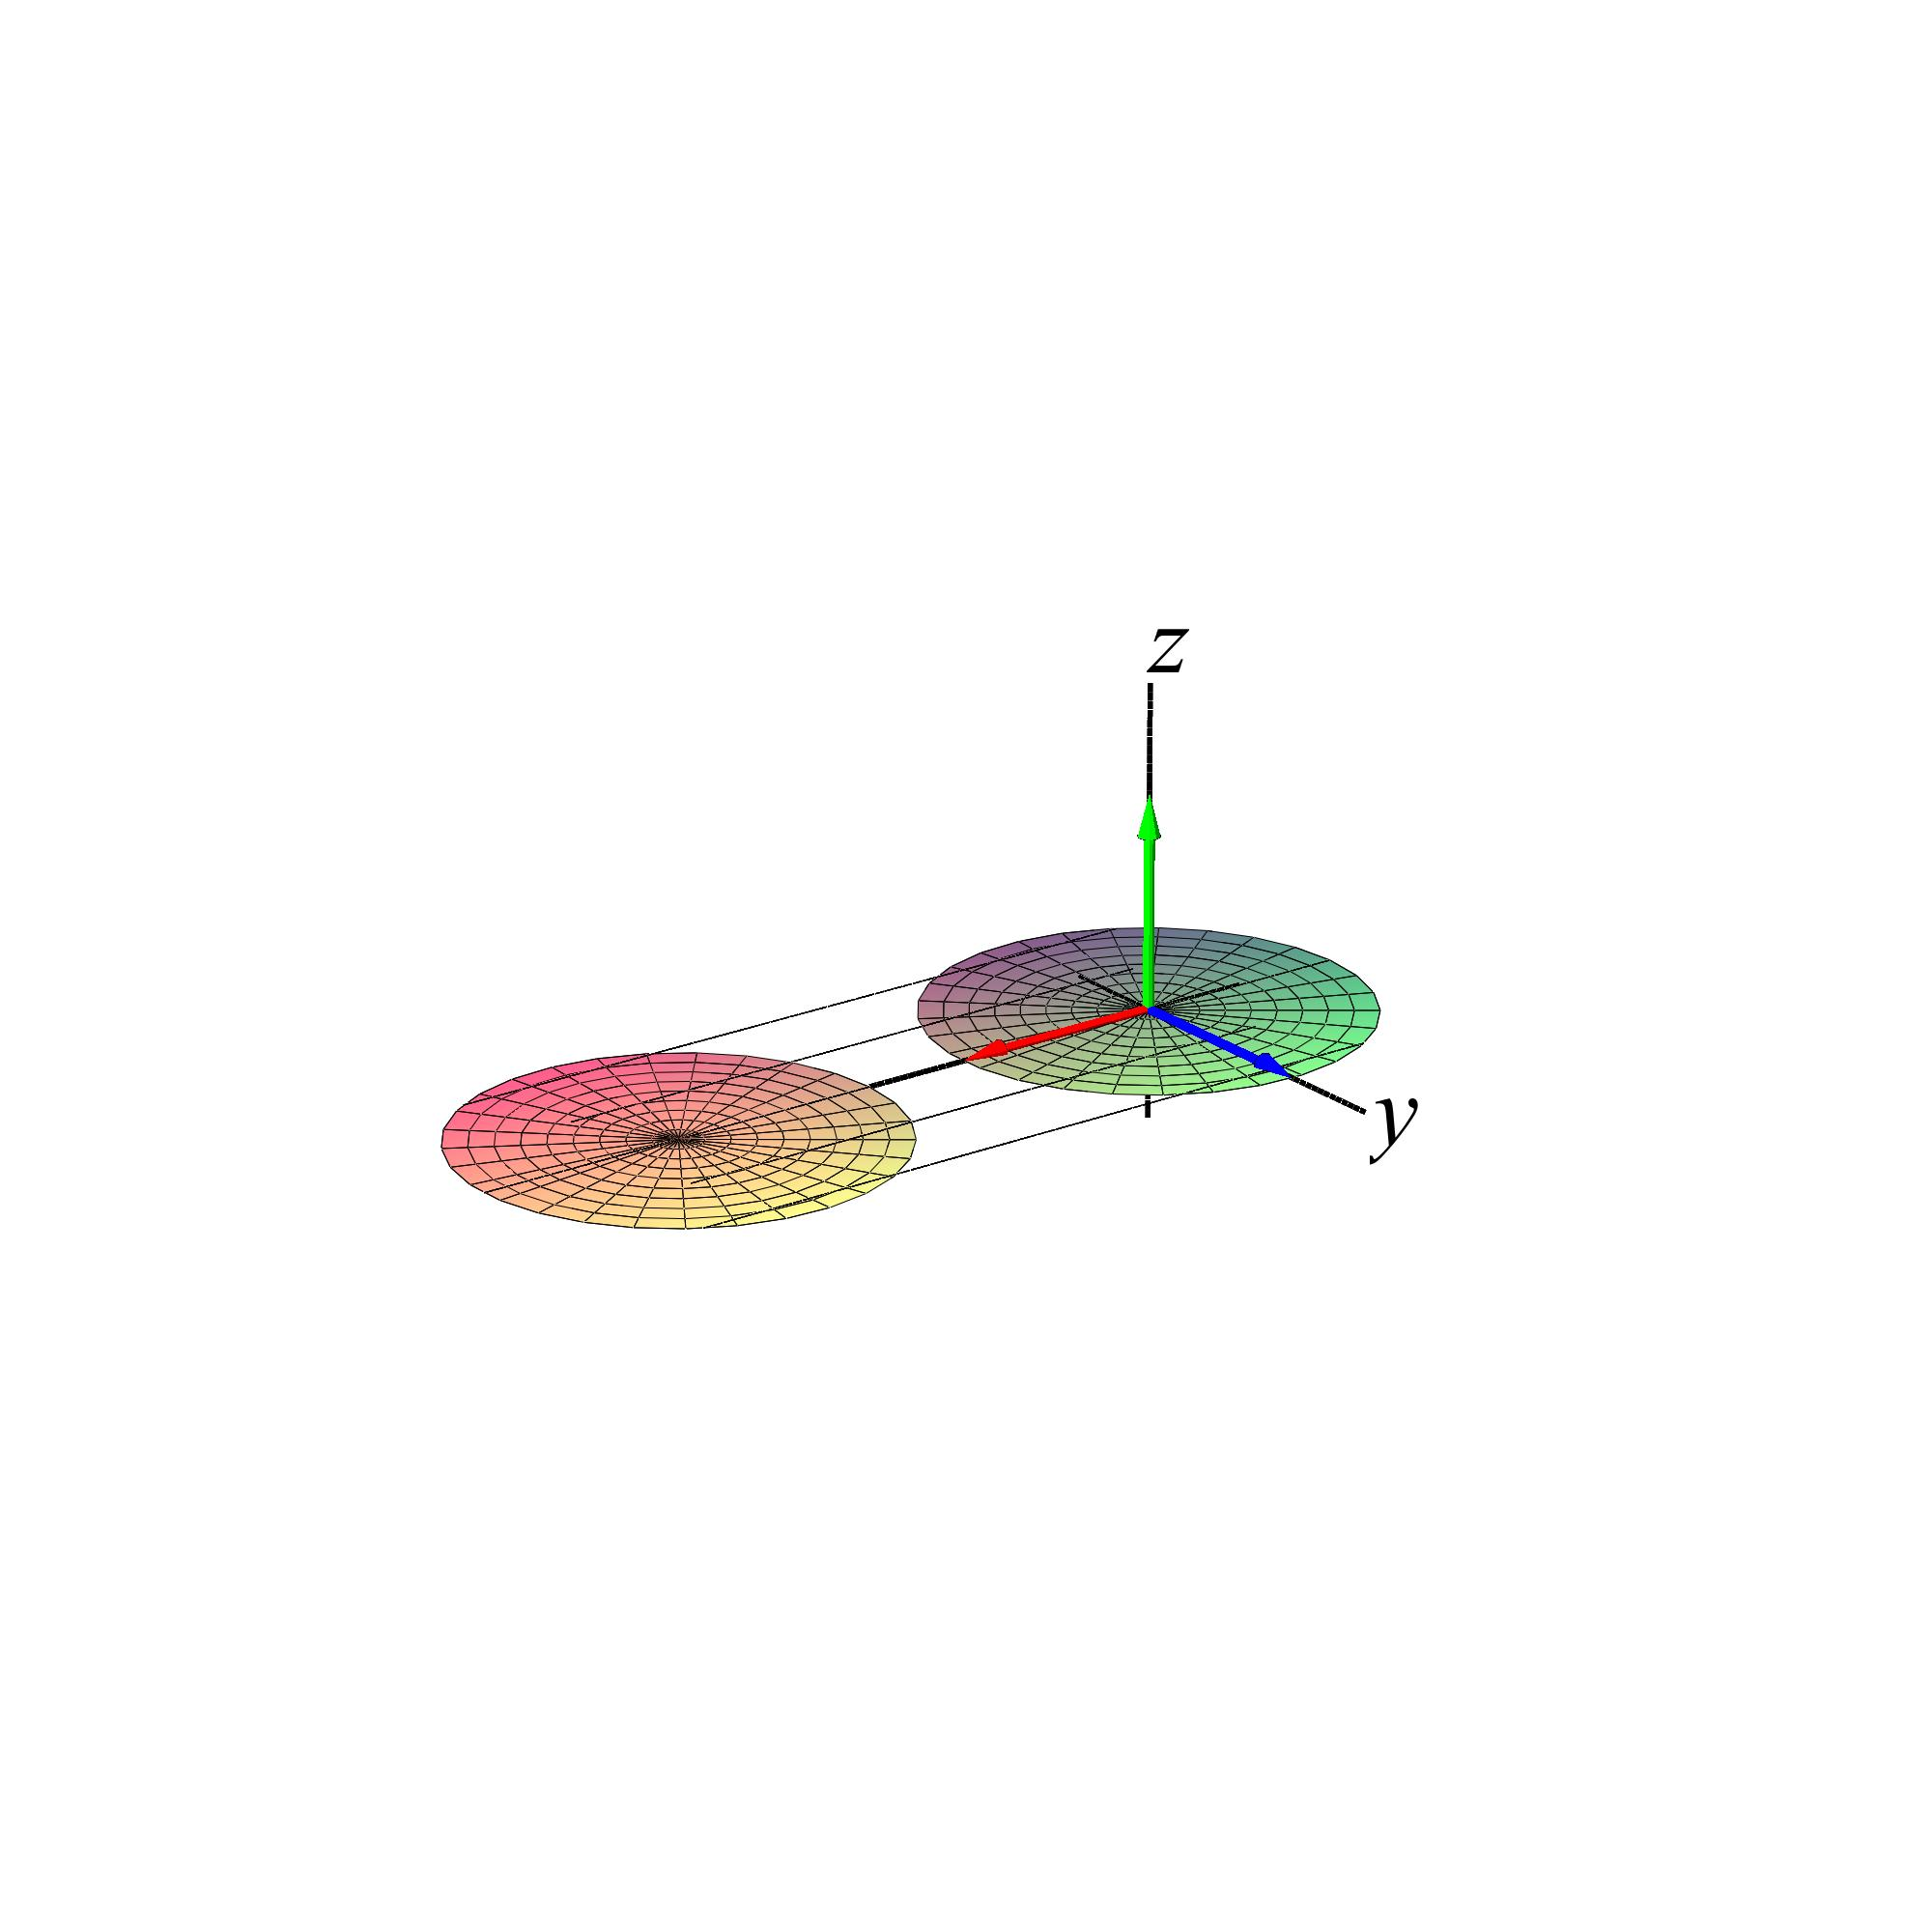
\includegraphics[width=70mm]{FIGS/plotSkiveFlowB2}}
\begin{center}
\caption{\small{Et simpelt, konstant vektorfelt, og tilsvarende kort-tids flow af en cirkelskive. Fluxen og volumen-tilvæksten er $0$. }} \label{figSkiveFlowB}
\end{center}
\end{figure}




\begin{example}[Flow af cirkelskive ved rotation] \label{exampSkiveFlowRot}
Vi ser som i eksempel \ref{exampFlowSkive1} på cirkelskiven $F_{\bf r}$ i $(x,y)$-planen. Skiven har  radius $1$ og centrum i $(0,0,0)$:
\begin{equation}
F_{\bf r} \quad : \quad {\bf r}(u,v) = (u\cdot \cos(v), u\cdot \sin(v), 0) \quad , \quad  (u,v) \in [0,1]\times [-\pi, \pi] \quad .
\end{equation}
Vi vil her lade cirkelskiven flyde med flowkurverne for følgende  roterende vektorfelt:
\begin{equation}
\mathbf{V}(x,y,z) = (-z,0, x) \quad .
\end{equation}
Flowkurven $\widetilde{\mathbf{r}}(u,v,t) = (x(t), y(t), z(t))$ for dette vektorfelt igennem et cirkelskive-punkt $(x_{0}, y_{0}, z_{0}) = \mathbf{r}(u,v)$ er givet som løsning til første-ordens differentialligningssystemet:
\begin{equation}
\left[
  \begin{array}{c}
    x'(t) \\
    y'(t) \\
    z'(t) \\
  \end{array}
\right] = (\mathbf{V}(x(t), y(t), z(t)))^{\top} = \left[
                                                    \begin{array}{c}
                                                     -z(t) \\
                                                      0 \\
                                                      x(t) \\
                                                    \end{array}
                                                  \right]
\end{equation}
med begyndelsesbetingelsen $(x(0), y(0), z(0) = (x_{0}, y_{0}, z_{0}) = \mathbf{r}(u,v)$.
Det koblede differentialligningssystem har de generelle løsninger, se løsningsmetoderne i \tref{NUID13-tn12}{eNote}:
\begin{equation}
\left[
  \begin{array}{c}
    x(t) \\
    y(t) \\
    z(t) \\
  \end{array}
\right]
  = \left[
  \begin{array}{c}
    c_{1}\cdot \cos(t) - c_{3}\cdot \sin(t) \\
    c_{2} \\
     c_{1}\cdot \sin(t) + c_{3}\cdot \cos(t) \\
  \end{array}
\right]
\end{equation}
hvor $c_{1}$, $c_{2}$, og $c_{3}$ er arbitrære konstanter.
De specielle løsninger, flowkurverne  $ \widetilde{\mathbf{r}}(u,v,t)$ igennem cirkelskivepunkterne $(x_{0}, y_{0}, z_{0}) = \mathbf{r}(u,v) = (u\cdot \cos(v), u\cdot \sin(v), 0)$ er så givet ved følgende parametriserede cirkler i rummet:
\begin{equation}
(\widetilde{\mathbf{r}}(u,v,t))^{\top} = \left[
                                           \begin{array}{c}
                                                x_{0}\cdot \cos(t) - z_{0}\cdot \sin(t) \\
    y_{0} \\
    x_{0}\cdot \sin(t) + y_{0}\cdot \cos(t) \\
                                           \end{array}
                                         \right] = \left[
                                           \begin{array}{c}
                                                u\cdot \cos(v)\cdot \cos(t) \\
    u\cdot \sin(v) \\
   u\cdot \cos(v)\cdot \sin(t)  \\
                                           \end{array}
                                         \right] \quad .
\end{equation}
 Det udfejede rumlige område  $\Omega_{F_{\mathbf{r}}}(t)$ er dermed allerede parametriseret:
 \begin{equation}
 \Omega_{F_{\mathbf{r}}}(t) \quad : \quad \widetilde{\mathbf{r}}(u,v,w) =
 (u\cdot \cos(v)\cdot \cos(w), \, u\cdot \sin(v), \,  u\cdot \cos(v)\cdot \sin(w) ) \quad ,
 \end{equation}
hvor $w \in [0, t]$, $u \in [0, 1]$, og $v \in [-\pi, \pi]$. Se figur \ref{figSkiveFlowRot}. \\


Fluxen af vektorfeltet igennem cirkelskiven forventes at være $0$ fordi det område, som cirkelskiven fejer igennem ved rotationen har \emph{rumfang} $0$ når rumfanget regnes med fortegn: Den ene halvdel af området ses jo at ligge \emph{over cirkelskiven} (i retning af $(0,0,1)$) og den anden halvdel ligger \emph{under cirkelskiven} (i retning af $(0,0,-1)$); de to halvdele af det udfejede område har rumfang med  modsatte fortegn og de ophæver derfor hinanden. Vi beregner fluxen af vektorfeltet igennem cirkelskiven:
\begin{equation}
\begin{aligned}
\Flux(\mathbf{V}, F_{\mathbf{r}}) &= \int_{-\pi}^{\pi} \int_{0}^{1} \mathbf{V}(\mathbf{r}(u,v)) \bm{\cdot} \mathbf{N}_{F}(u,v) \, \, du \, dv \\
&= \int_{-\pi}^{\pi} \int_{0}^{1} (0, 0, u\cdot \cos(v))  \bm{\cdot}(0,0,u) \, \, du \, dv \\
&= \int_{-\pi}^{\pi} \int_{0}^{1} u^{2} \cdot \cos(v) \, \, du \, dv \\
&= \int_{-\pi}^{\pi} \frac{1}{3} \cdot \cos(v) \, \, dv \\
&= \frac{1}{3} \cdot \int_{-\pi}^{\pi} \cos(v) \, \, dv \\
&= \frac{1}{3} \cdot \left[\sin(v) \right]_{-\pi}^{\pi} \\
&= 0 \quad .
\end{aligned}
\end{equation}

Med henblik på igen at illustrere den generelle rumfangsberegning (med fortegn) og igen verificere sætning \ref{thmFluxVolEkspand} med konkrete udregninger, vil vi vise, at det med fortegn beregnede rumfang af området $\Omega_{F_{\mathbf{r}}}(t)$  som fejes ud af cirkelskiven ved flowet virkelig er $0$. Den med fortegn beregnede Jacobifunktion er bestemt ved:
\begin{equation}
\Jac_{\widetilde{\mathbf{r}}}(u,v,w) = u^{2}\cdot \cos(v) \quad .
\end{equation}
sådan at det fortegns-vægtede volumen af $\Omega_{F_{\mathbf{r}}}(t)$ er:
\begin{equation}
\begin{aligned}
\Vol_{\pm}(\Omega_{F_{\mathbf{r}}}(t)) &= \int_{0}^{t} \int_{-\pi}^{\pi} \int_{0}^{1} u^{2}\cdot \cos(v) \, \, du \, dv \, dw \\
&= \frac{1}{3}\cdot \int_{0}^{t} \int_{-\pi}^{\pi}\cdot \cos(v) \, \, dv \, dw \\
&= \frac{1}{3}\cdot t \cdot \left[ \sin(v)\right]_{-\pi}^{\pi} \\
&= 0 \quad .
\end{aligned}
\end{equation}
Bemærk, at det ordinære rumfang $\Vol(\Omega_{F_{\mathbf{r}}}(t))$   af $\Omega_{F_{\mathbf{r}}}(t)$ selvfølgelig ikke er $0$, men derimod:
\begin{equation}
\begin{aligned}
\Vol(\Omega_{F_{\mathbf{r}}}(t)) &= \int_{0}^{t} \int_{-\pi}^{\pi} \int_{0}^{1} u^{2}\cdot |\cos(v)| \, \, du \, dv \, dw \\
&= \frac{1}{3}\cdot \int_{0}^{t} \int_{-\pi}^{\pi} |\cos(v)| \, \, dv \, dw \\
&= \frac{1}{3}\cdot t \cdot 4 \cdot \left[ \sin(v)\right]_{0}^{\pi/2} \\
&= \frac{4}{3}\cdot t \quad .
\end{aligned}
\end{equation}
\end{example}

\begin{figure}[ht]
\centerline{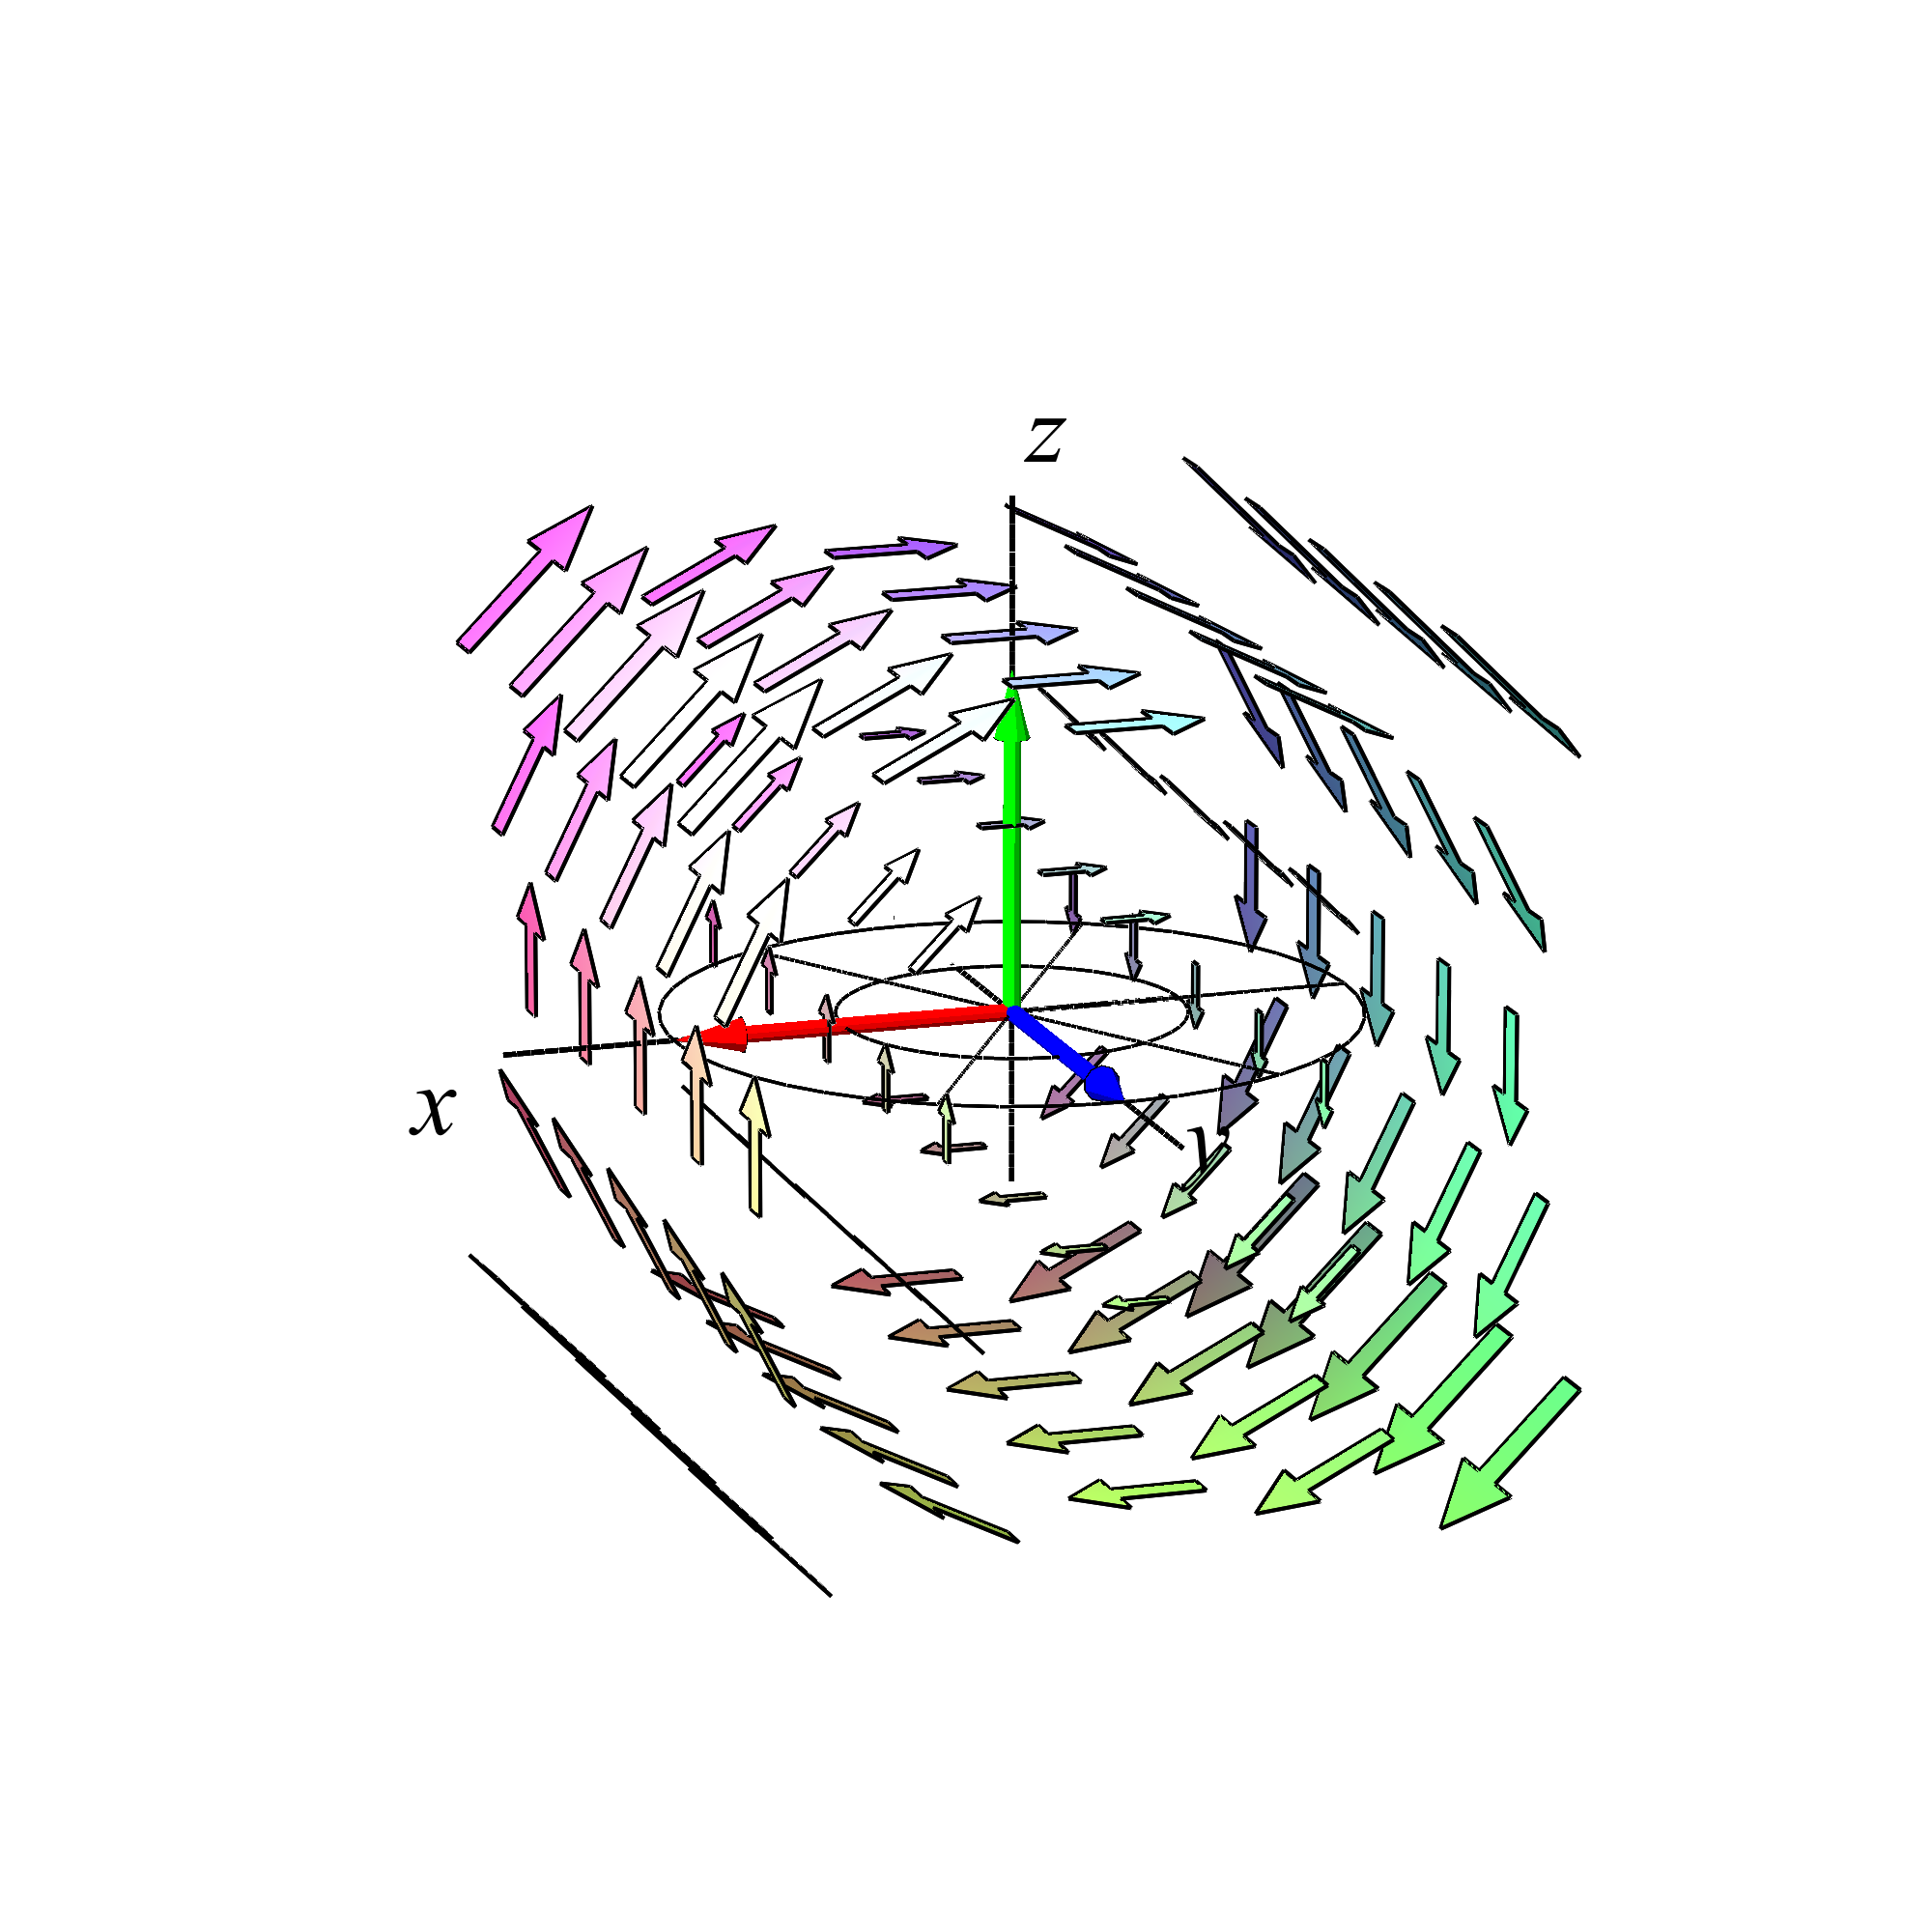
\includegraphics[width=70mm]{FIGS/plotSkiveFlowRot1}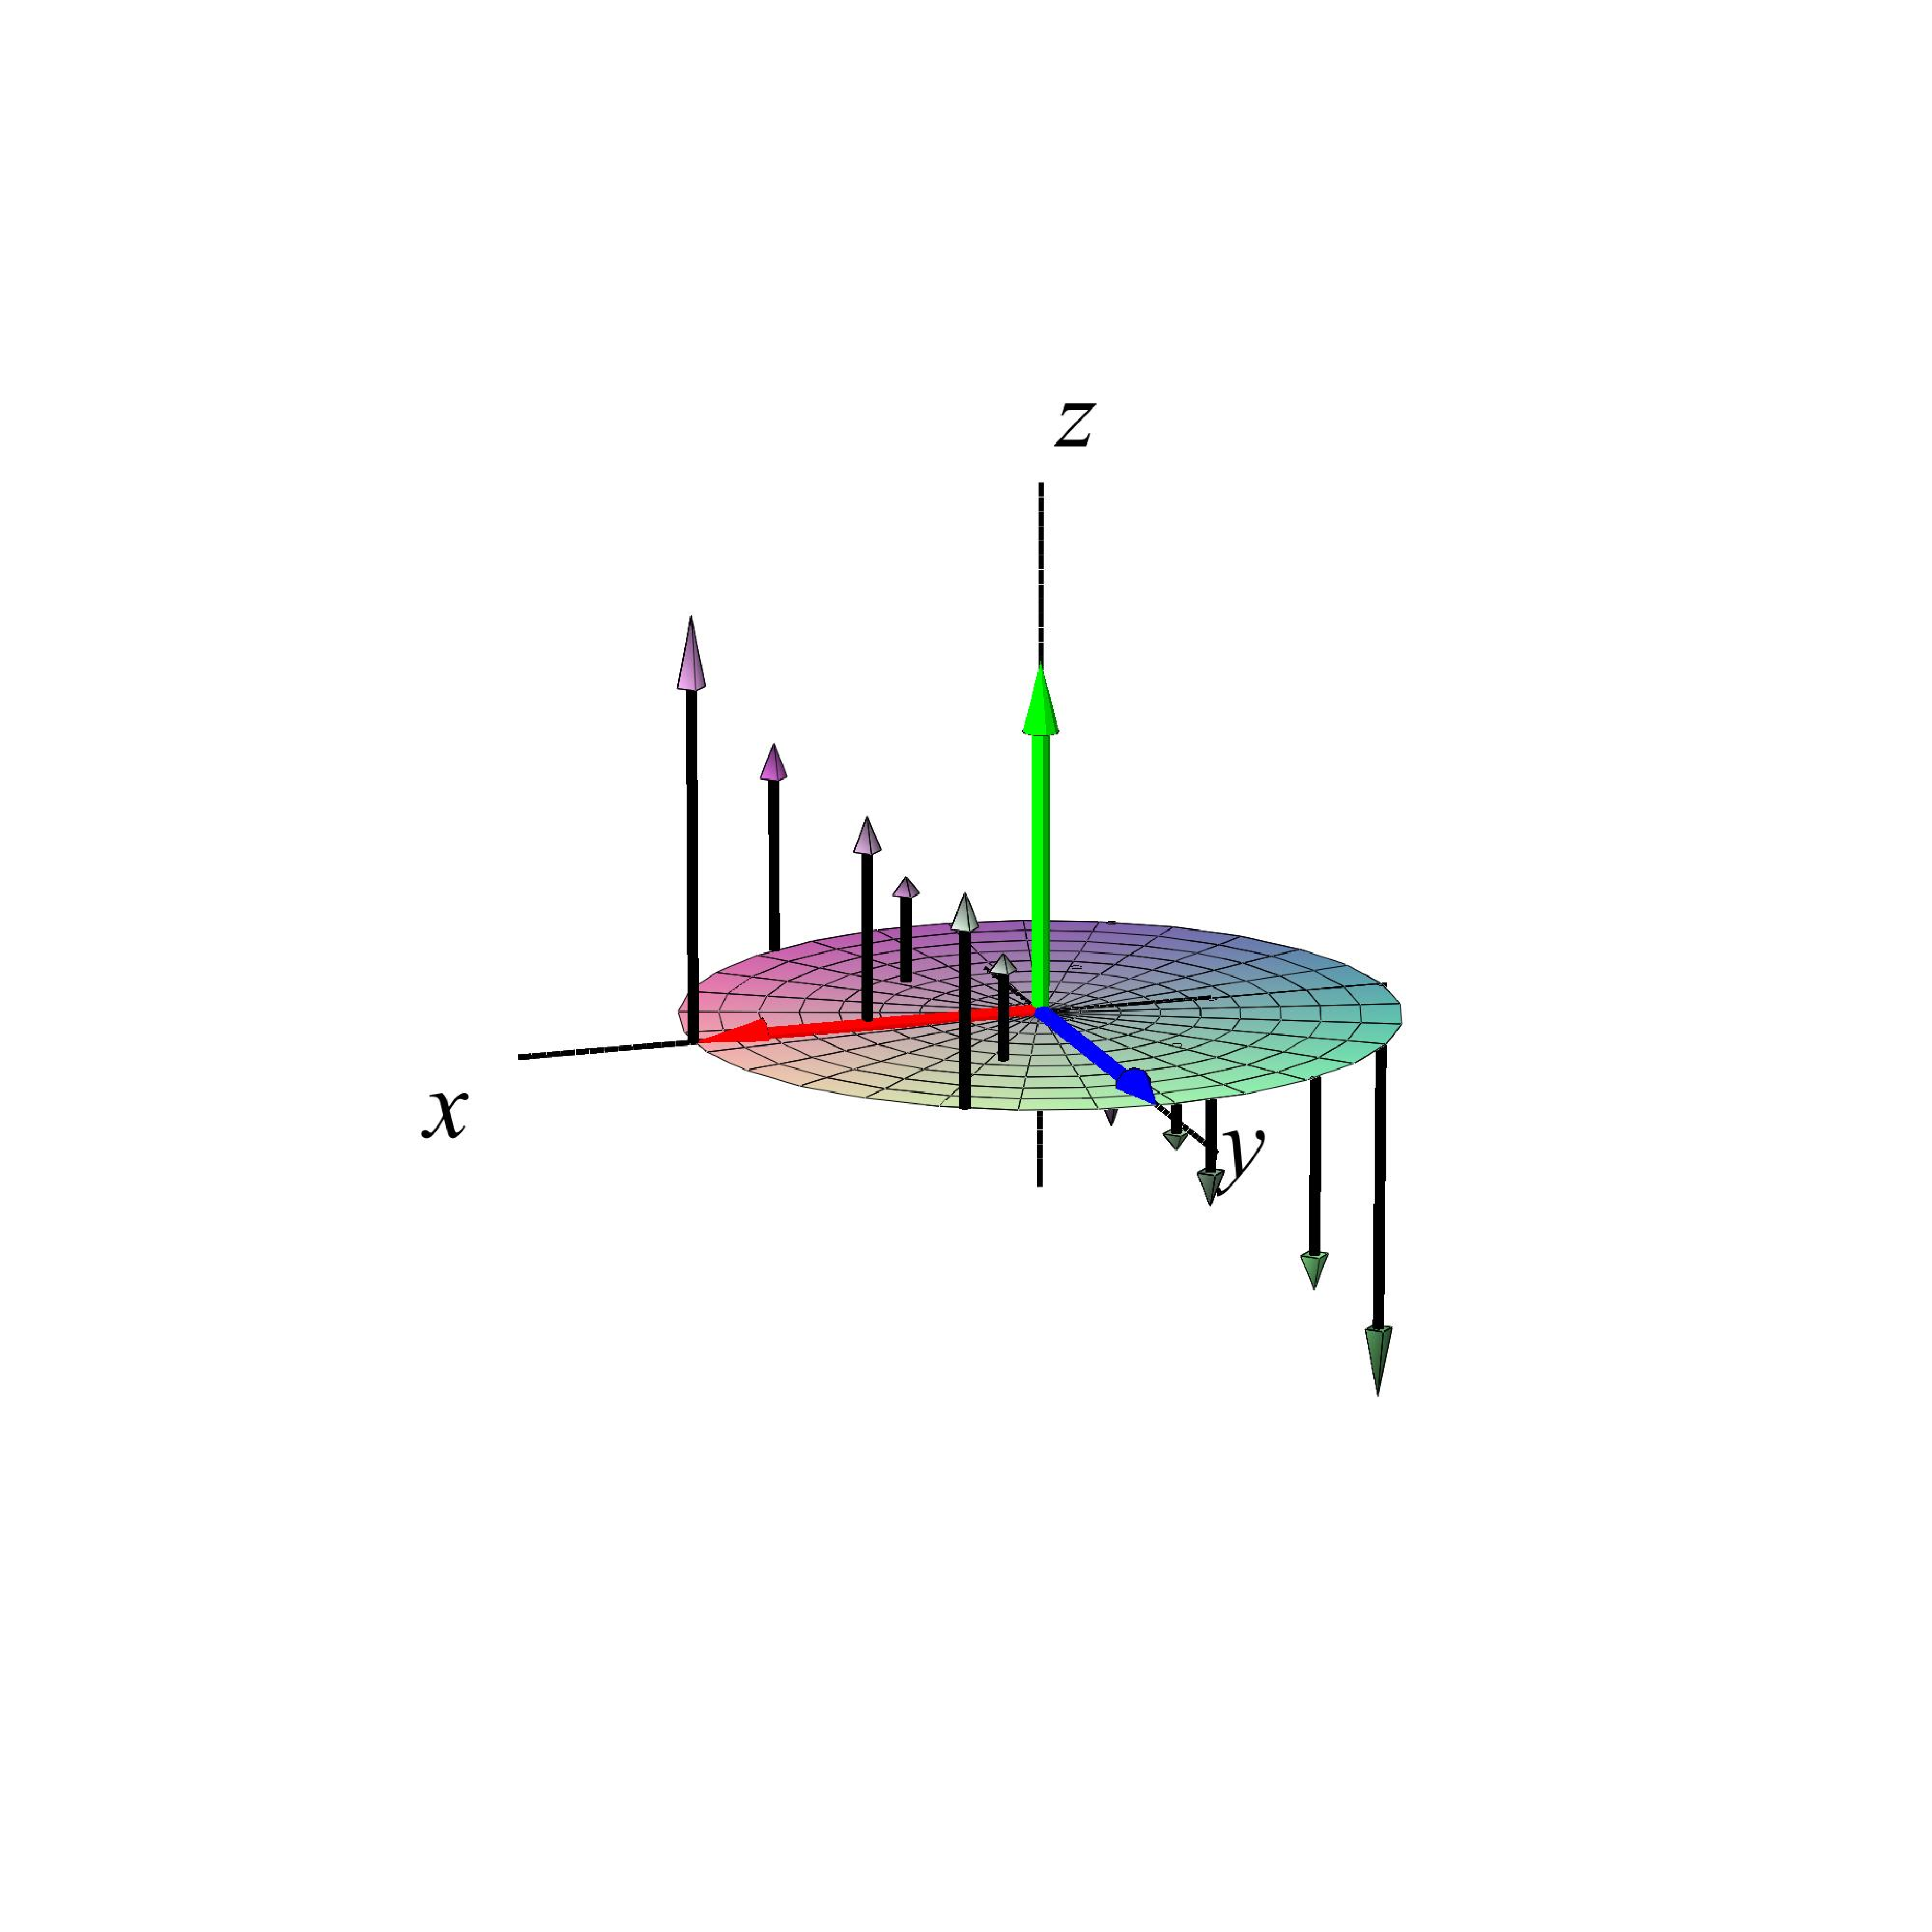
\includegraphics[width=70mm]{FIGS/plotSkiveFlowRot3}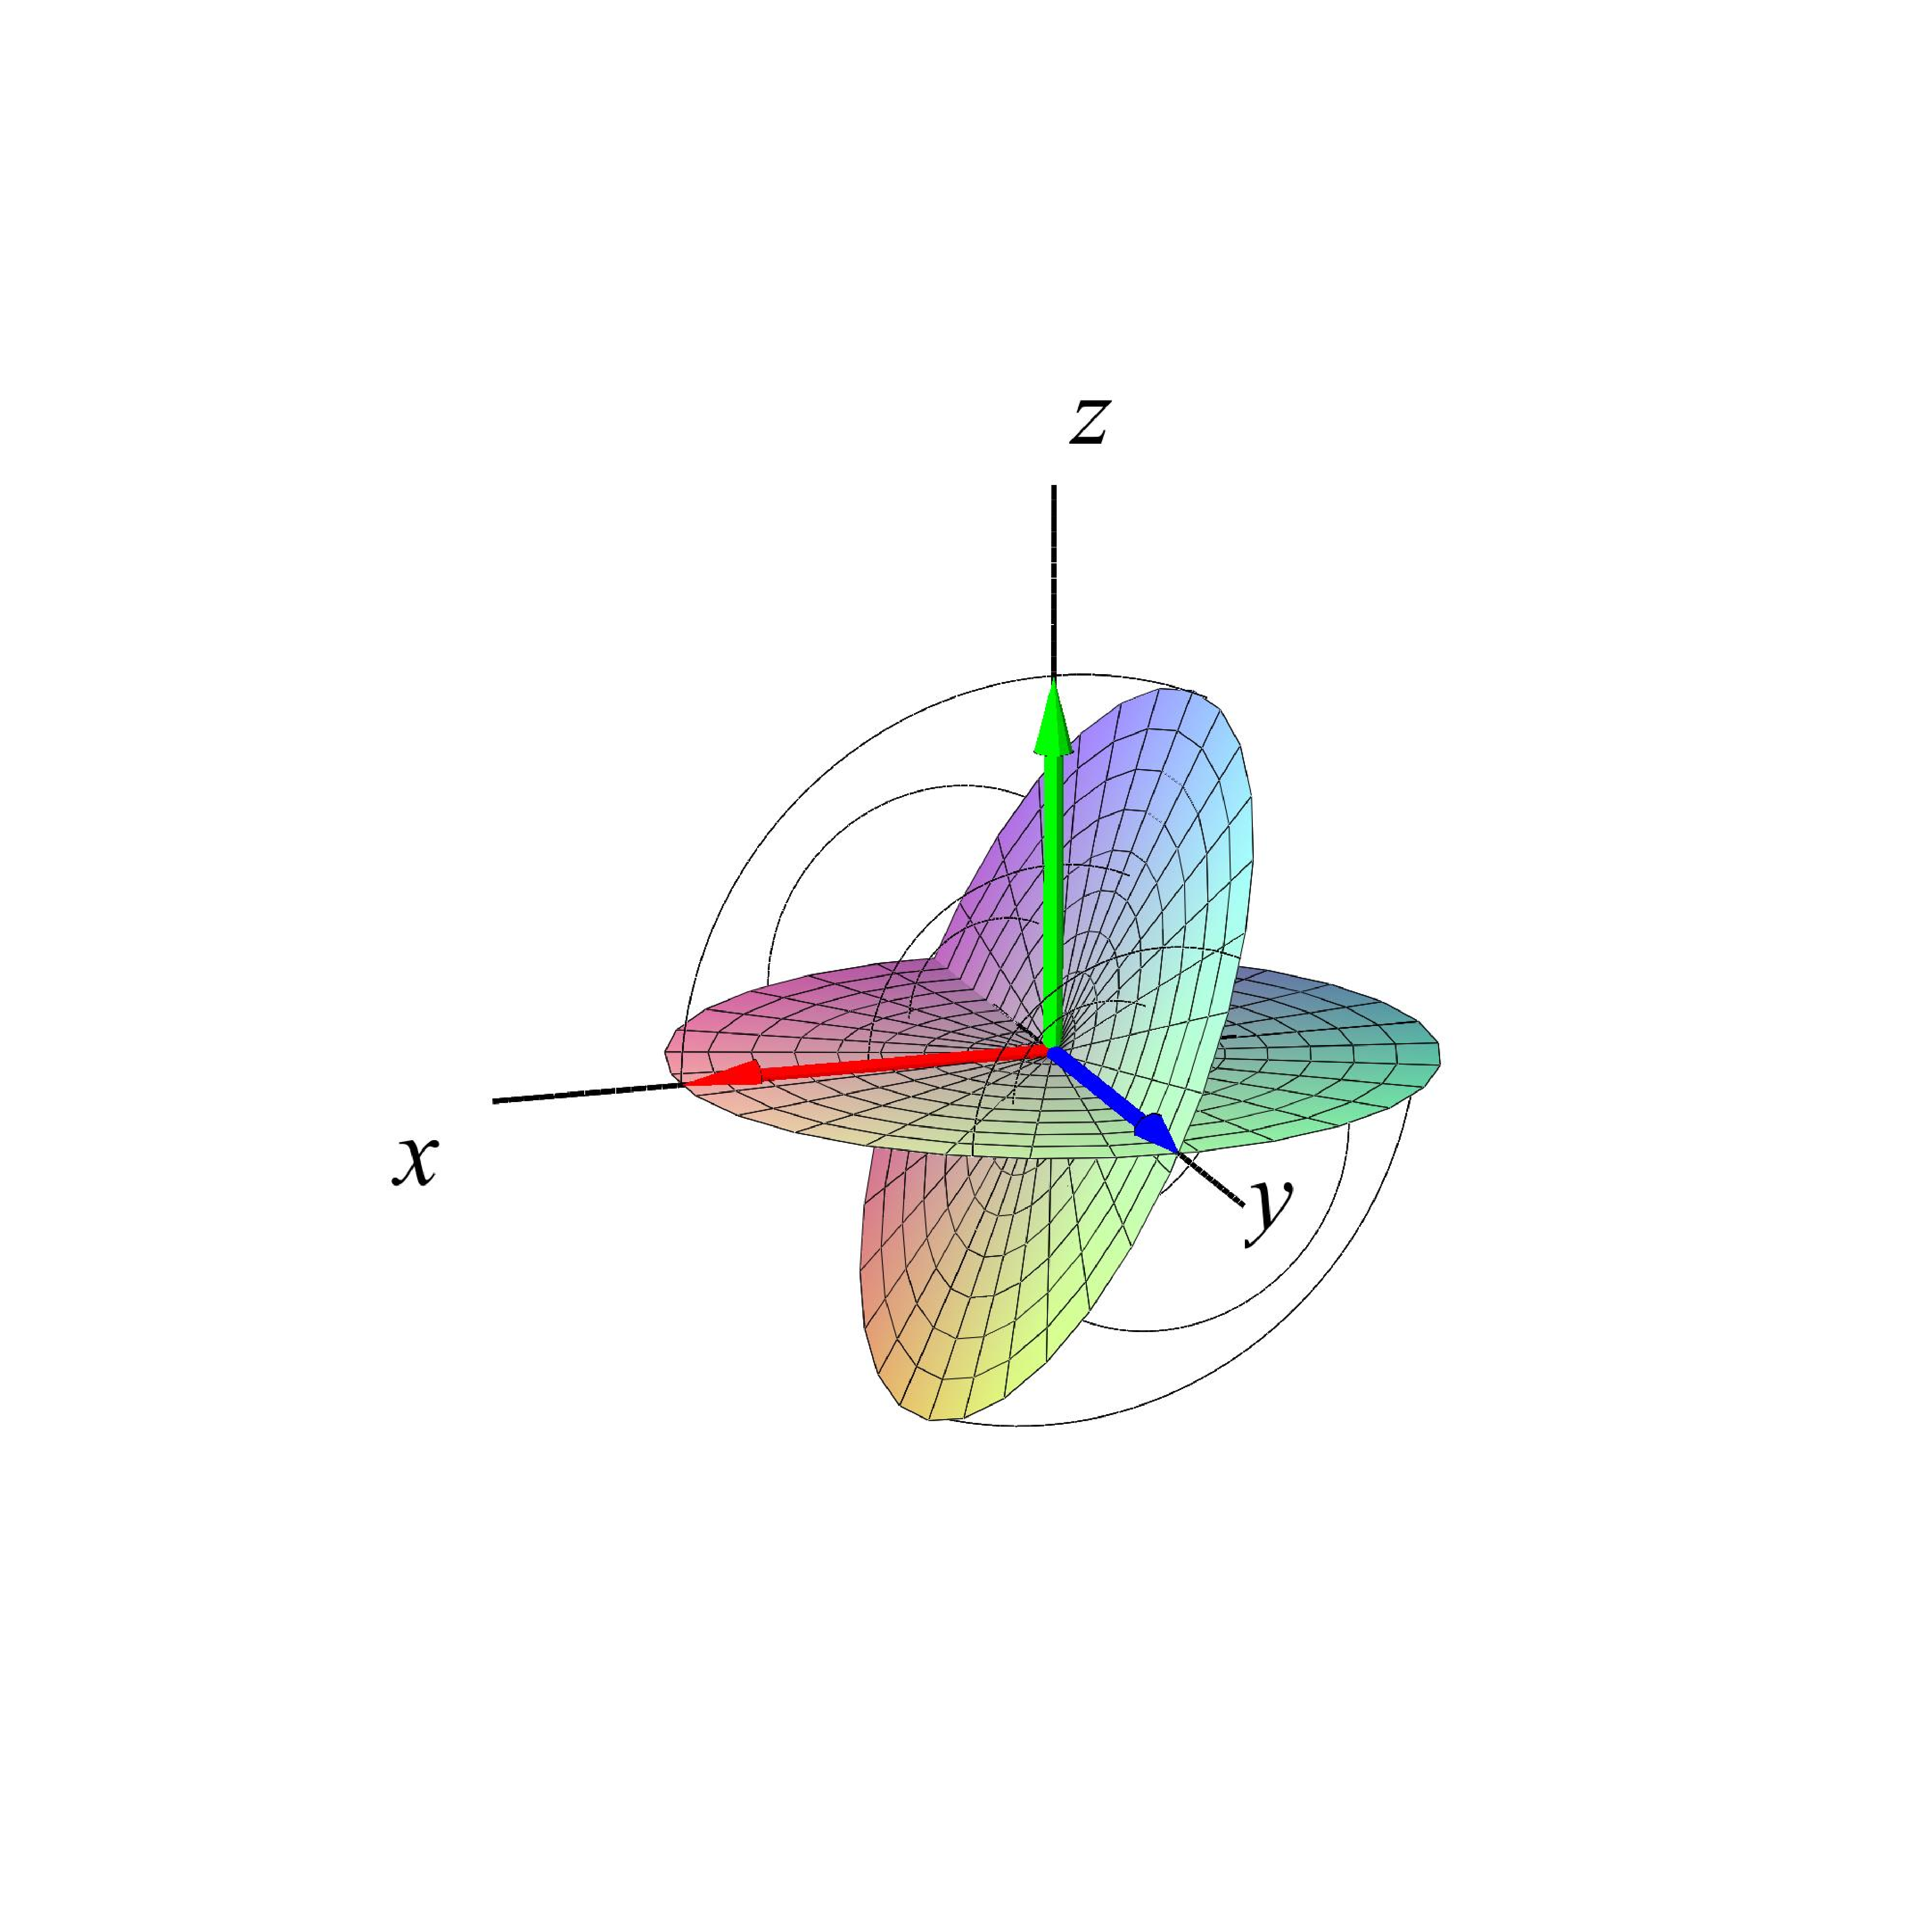
\includegraphics[width=70mm]{FIGS/plotSkiveFlowRot2}}
\begin{center}
\caption{\small{Et roterende vektorfelt og tilsvarende kort-tids flow af en cirkelskive. Fluxen og volumen-tilvæksten er $0$. }} \label{figSkiveFlowRot}
\end{center}
\end{figure}










\begin{example}[Flux gennem en elliptisk paraboloide]\label{exampParabFlux}
Et vektorfelt $\mathbf{V}(x,y,z)$ og en elliptisk paraboloide $F_{\mathbf{r}}$ er givet ved henholdsvis
\begin{equation}
\mathbf{r}(u,v) = \left(2\cdot u\cdot \cos(v), 2\cdot u\cdot \sin(v), 2\cdot u^{2} \cdot (\cos^{2}(v) + \frac{1}{9}\cdot \sin^{2}(v)) \right) \quad ,
\end{equation}
hvor $(u,v) \in [0, 1/2] \times [-\pi, \pi]$, og $\mathbf{V}(x,y,z) = (-y, x, 1)$. \\

Til bestemmelse af fluxen $\Flux(\mathbf{V}, F_{\mathbf{r}})$ af $\mathbf{V}(x,y,z)$ gennem $F_{\mathbf{r}}$ har vi
\begin{equation}
\mathbf{r}_{u}(u,v) \times \mathbf{r}_{v}(u,v) = \left(-8\cdot u^{2} \cdot \cos(v), \, -\frac{8}{9}\cdot u^{2} \cdot \sin(v) , \, 4\cdot u)\right)
\end{equation}
\begin{equation}
\mathbf{V}(\mathbf{r}(u,v)) = (-2\cdot u \cdot \sin(v), 2\cdot u \cdot \cos(v), 1) \quad .
\end{equation}
sådan at:
\begin{equation}
\begin{aligned}
\Flux(\mathbf{V}, F_{\bf r}) &= \int_{-\pi}^{\pi} \int_{0}^{1/2} \mathbf{V}(\mathbf{r}(u,v)) \bm{\cdot} ( {\bf r}_{u}(u,v) \times {\bf r}_{v}(u,v)) \, \, du \, dv \\
&= \int_{-\pi}^{\pi} \int_{0}^{1/2} \frac{4}{9}\cdot u \cdot \left(32\cdot u^{2}\cdot \cos(v)\cdot \sin (v) + 9 \right)  \, \, du \, dv \\
&= \cdots \\
&= \pi \quad.
\end{aligned}
\end{equation}
\end{example}

\begin{figure}[ht]
\centerline{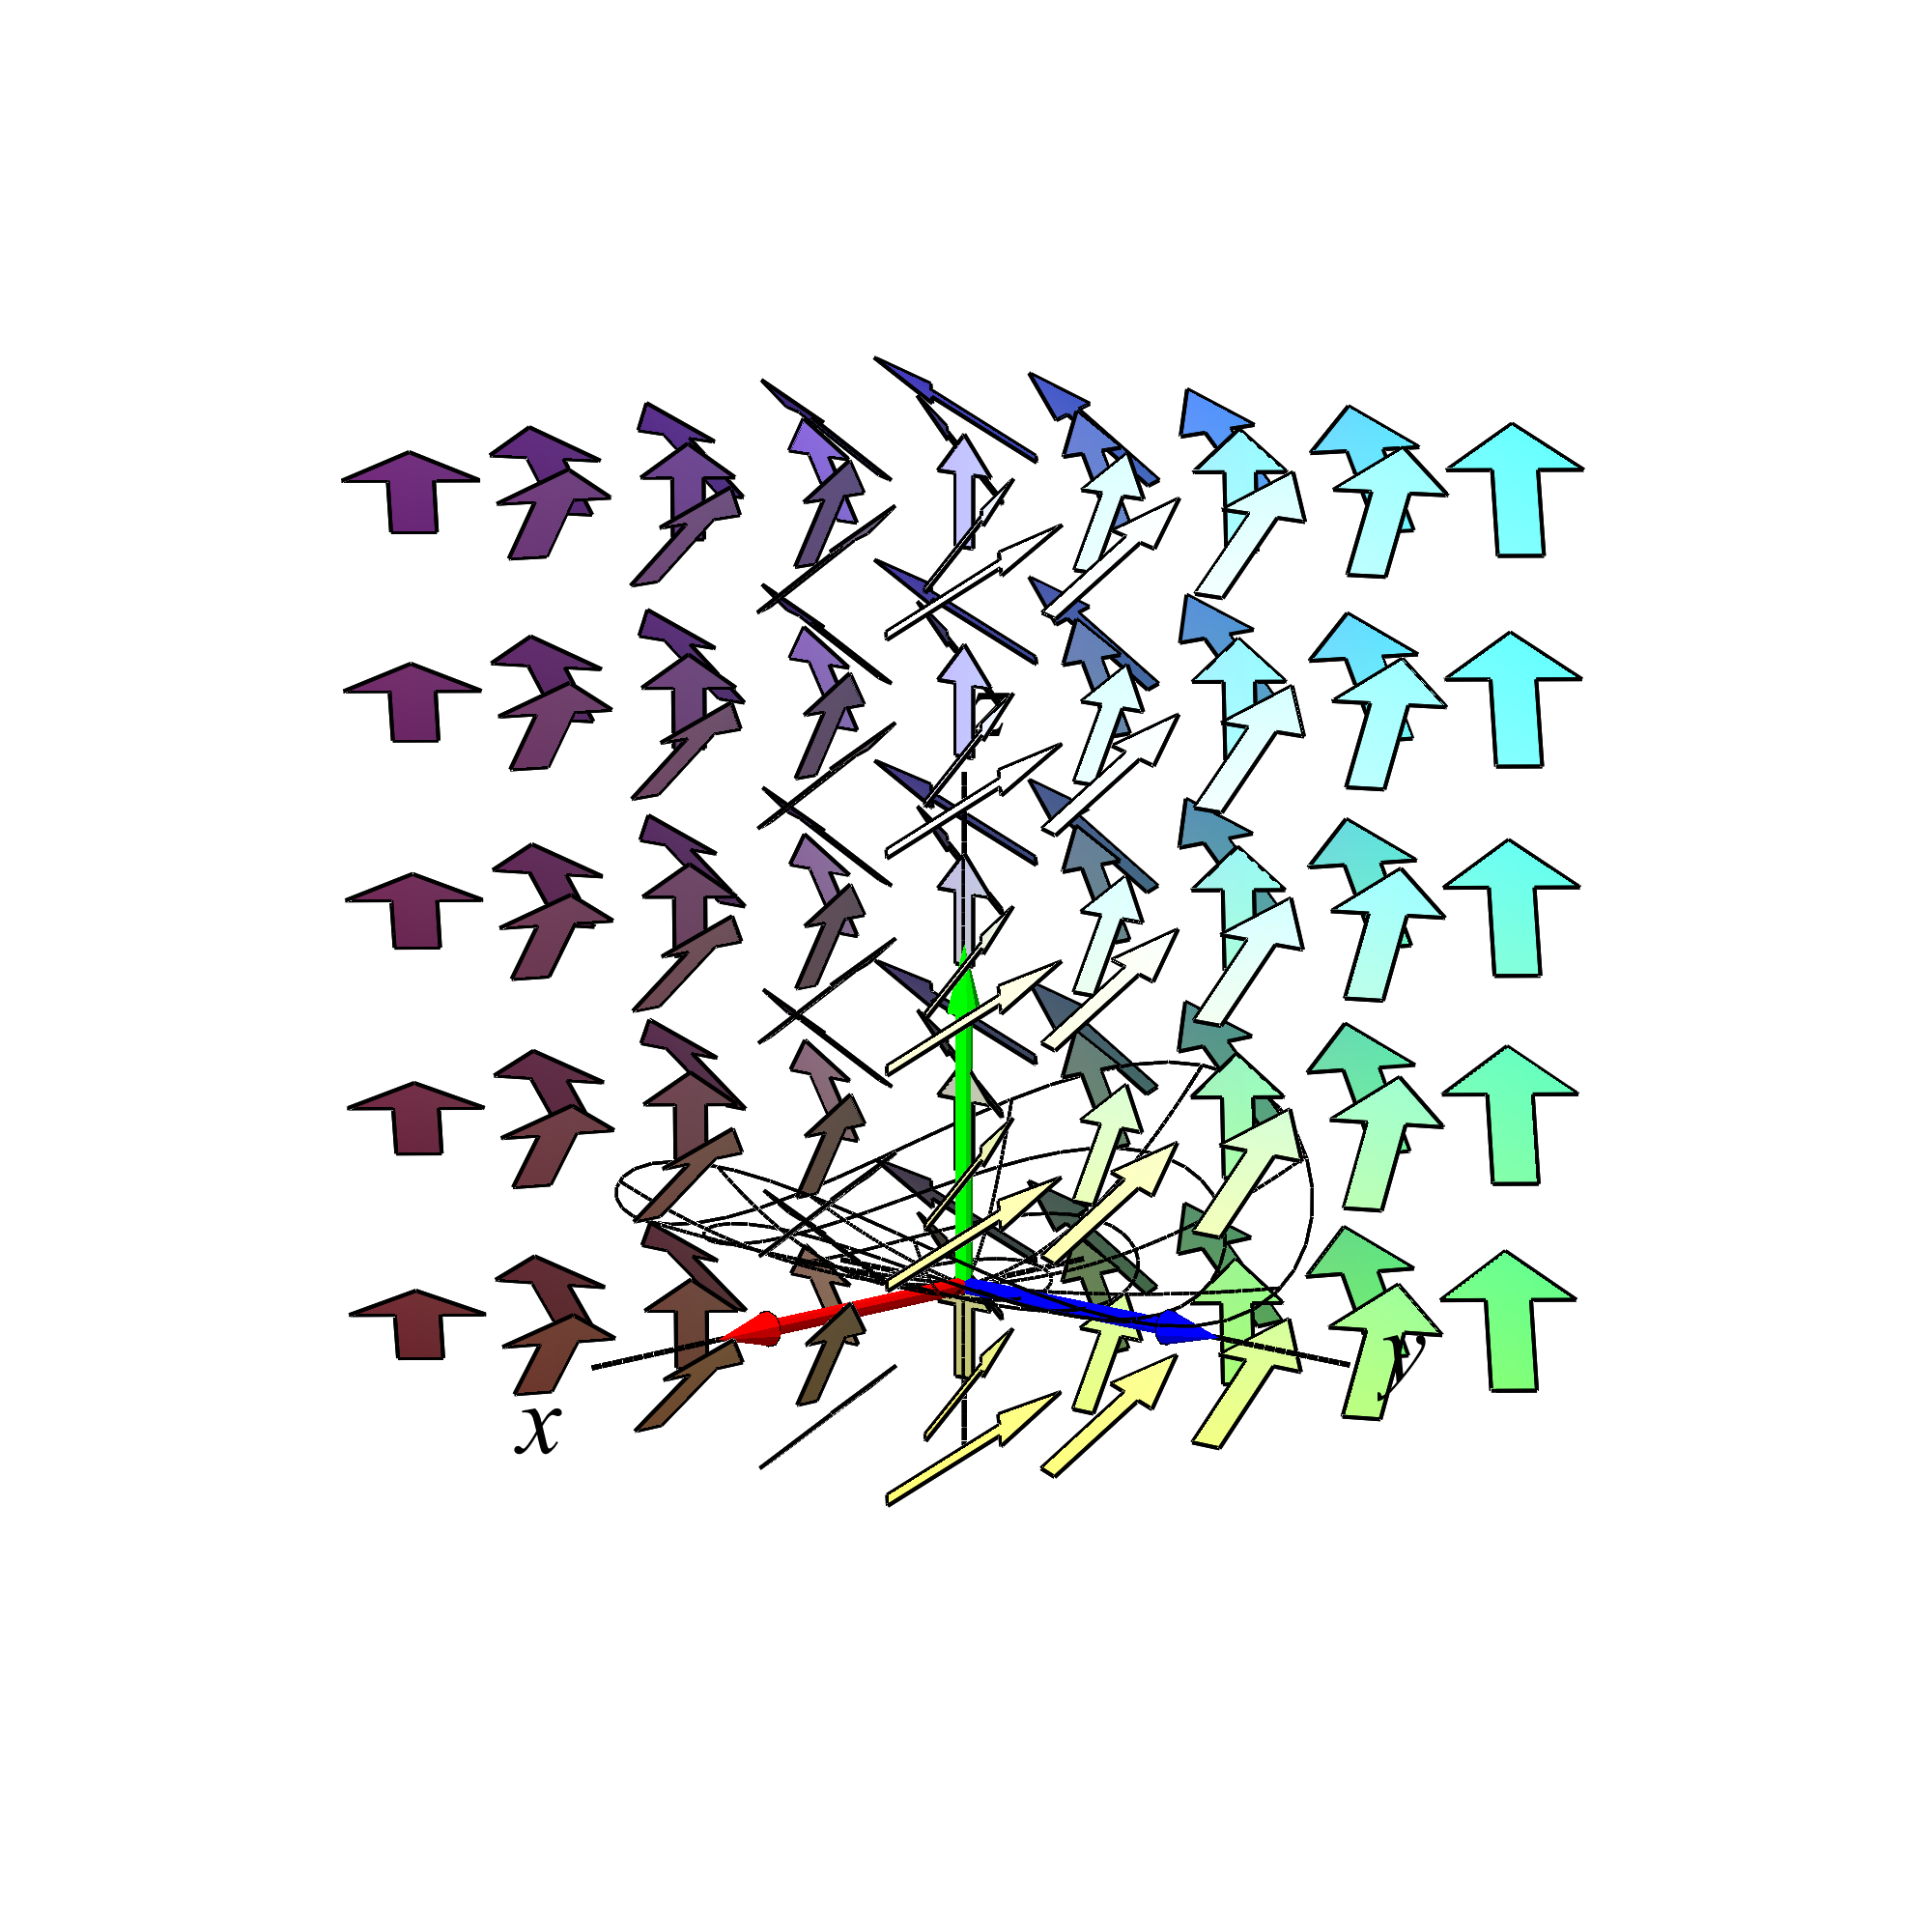
\includegraphics[width=70mm]{FIGS/plotParabFlowA1}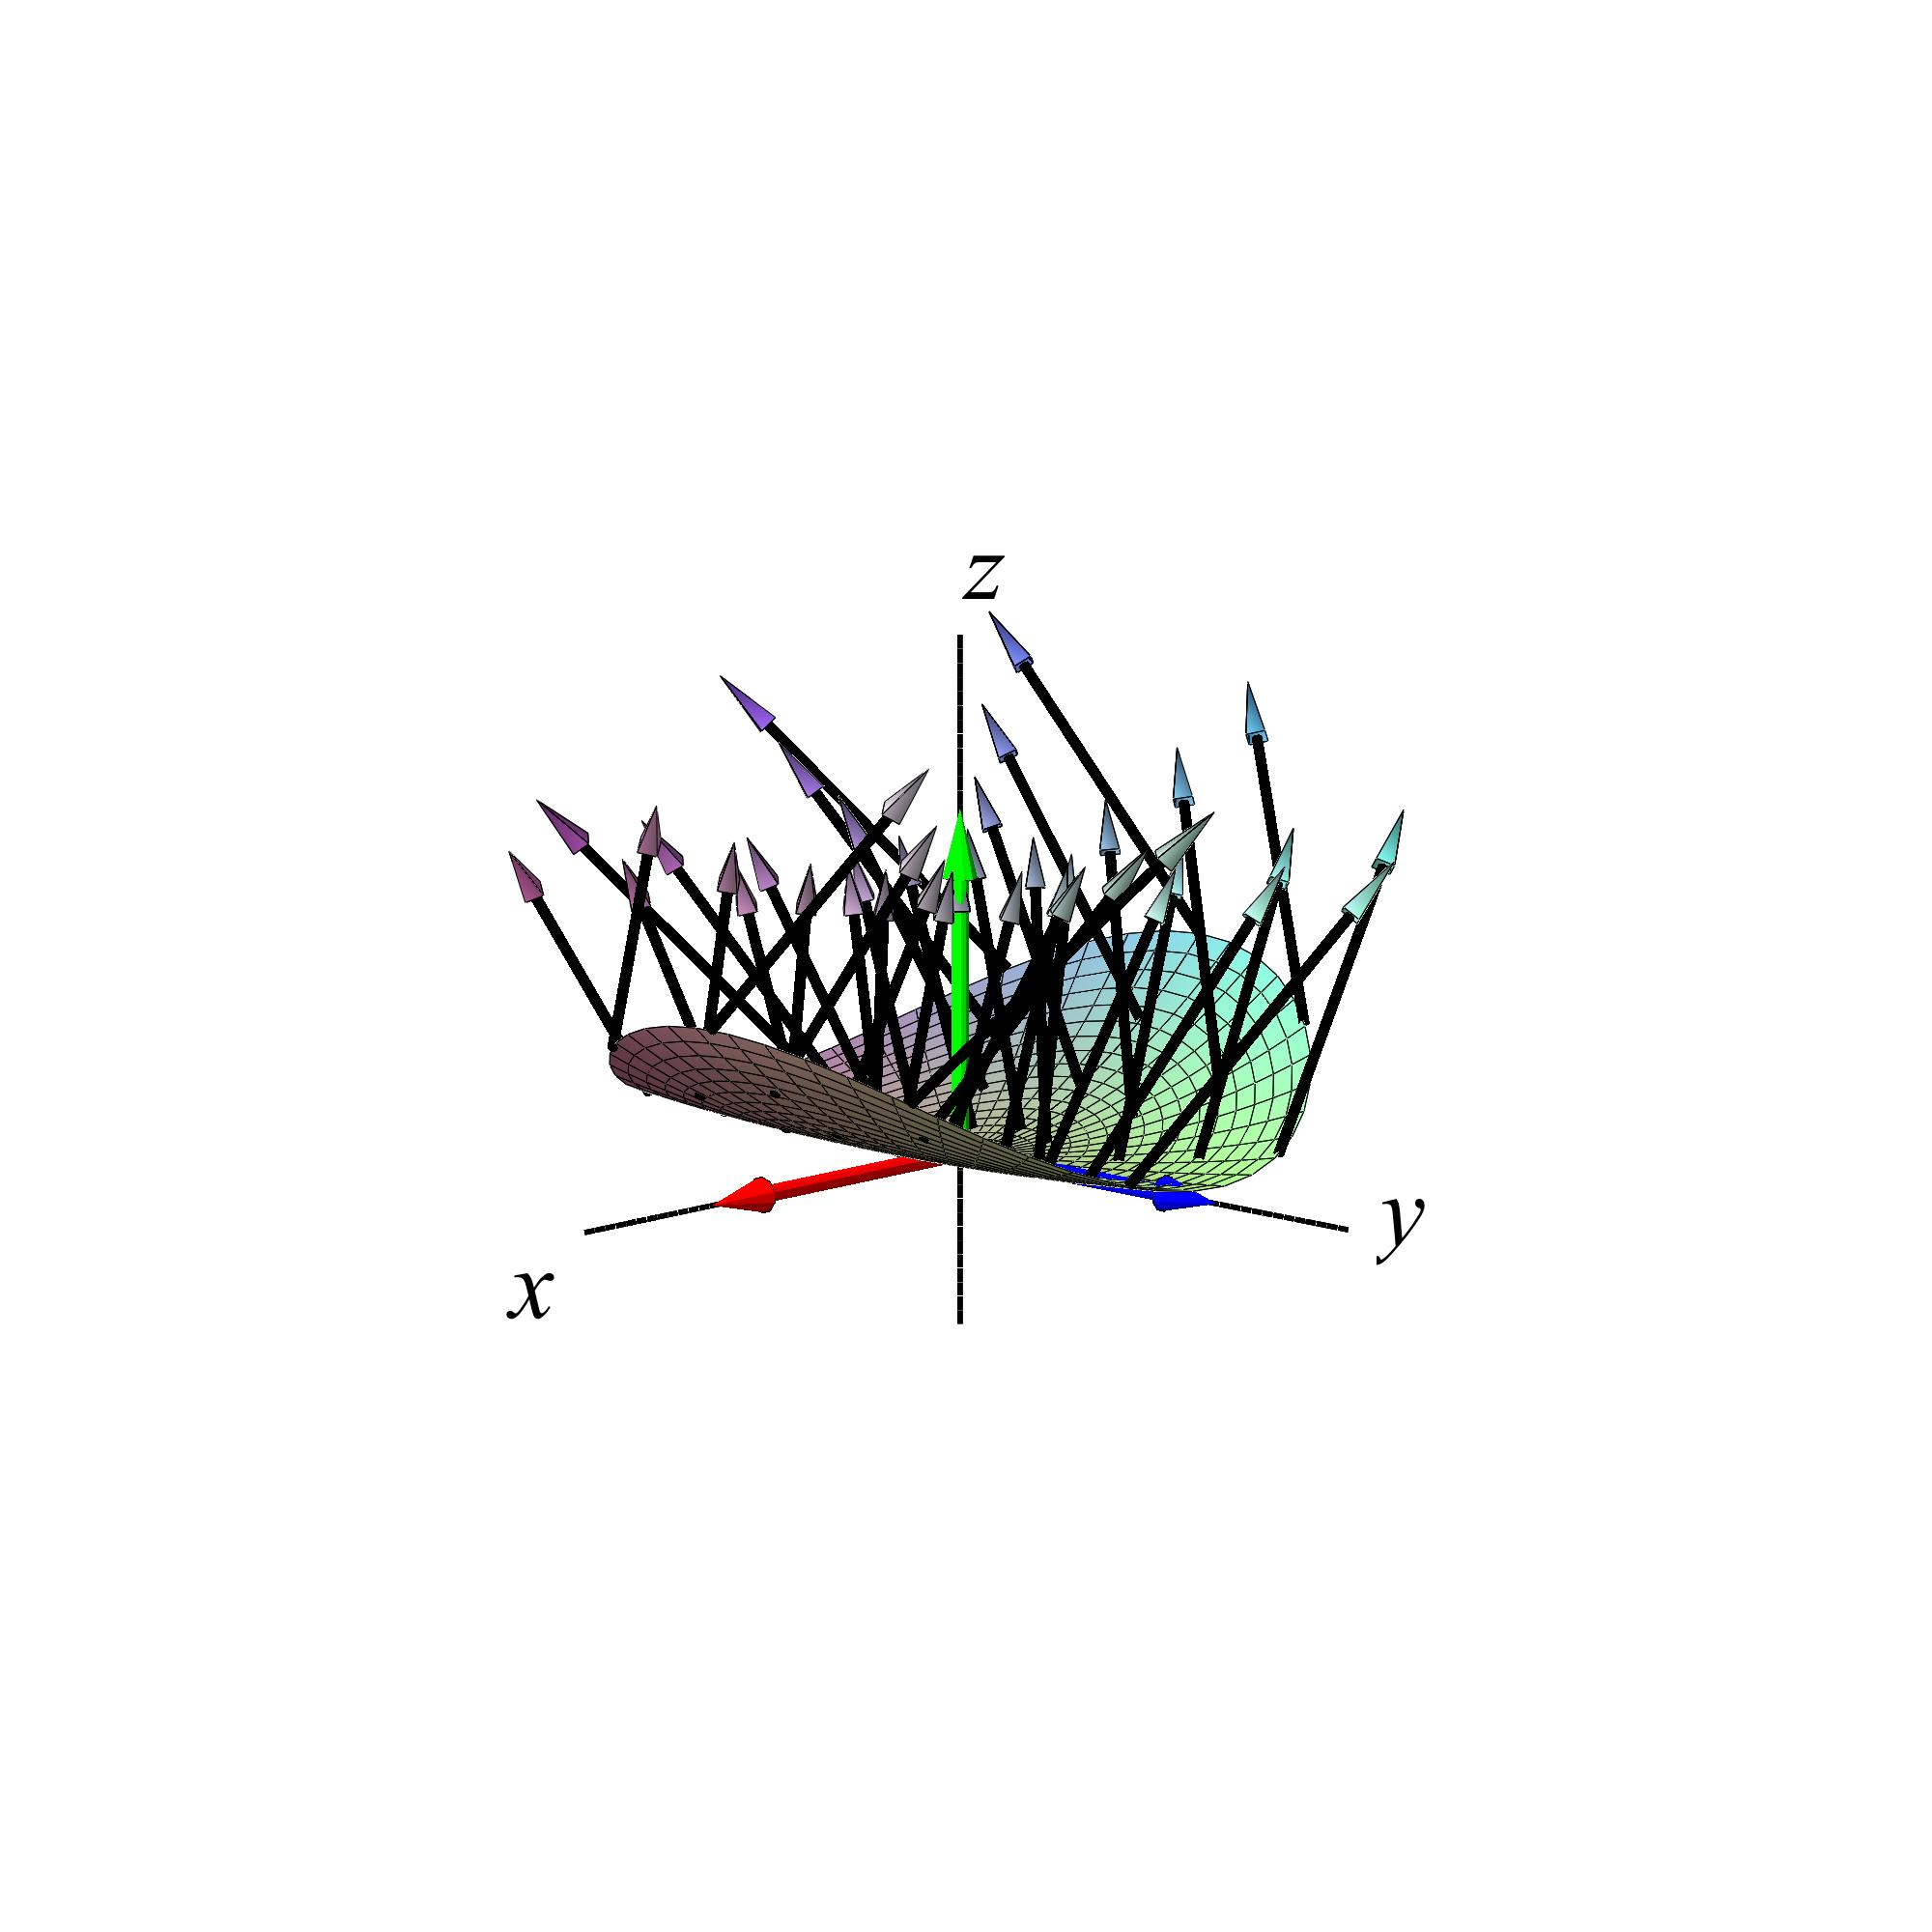
\includegraphics[width=70mm]{FIGS/plotParabFlowA3}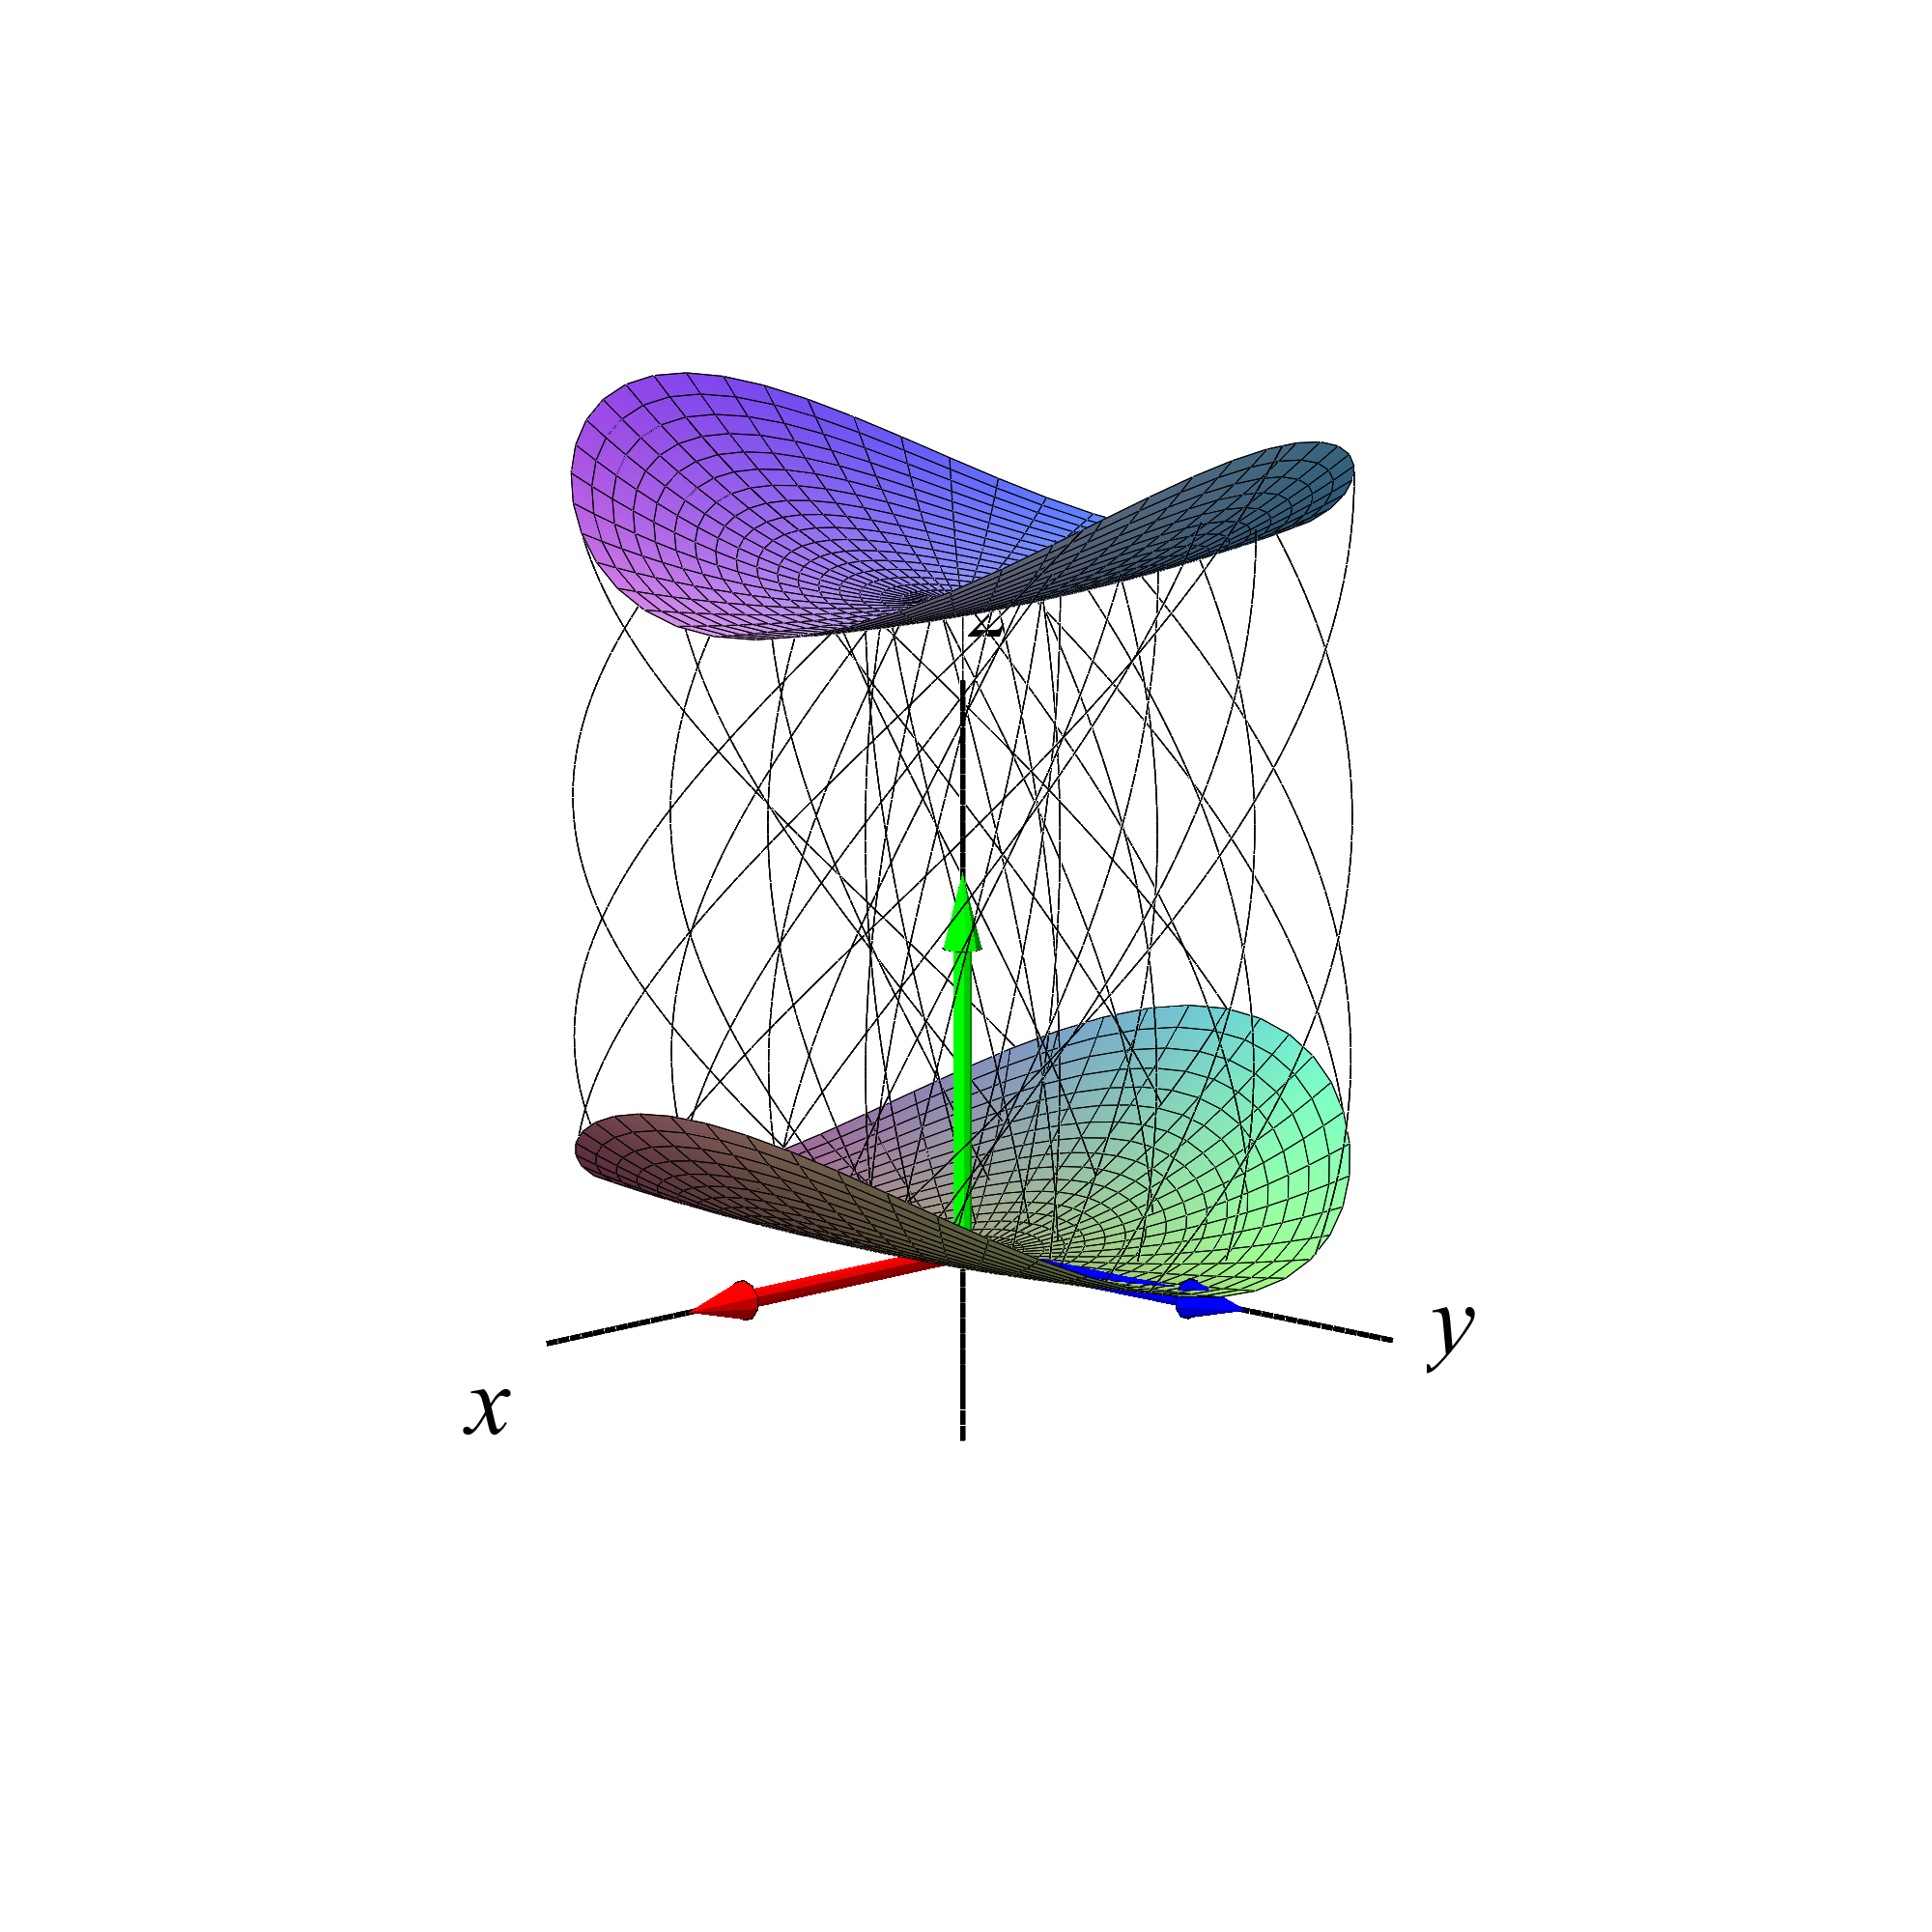
\includegraphics[width=70mm]{FIGS/plotParabFlowA2}}
\begin{center}
\caption{\small{Et roterende vektorfelt, og tilsvarende kort-tids flow af en elliptisk paraboloide. I forhold til cirkelskivenormalen er fluxen og volumen-tilvæksten positiv. Se eksempel \ref{exampParabFlux}.}} \label{figParabFlow}
\end{center}
\end{figure}


Som vi skal se i næste afsnit er den totale flux af et givet vektorfelt gennem \emph{overfladen} af et givet rumligt område $\Omega_{\mathbf{r}}$ særlig interessant. Overfladen kan gerne være sammensat af endeligt mange glatte fladestykker, som f.eks. overfladen af et polyeder. Den eneste konvention vi skal holde os for øje er, at det altid er den \emph{udadrettede normal} (i forhold til det rumlige område) vi skal benytte overalt på overfladen, når vi beregner fluxen.


\begin{example}[Flux gennem overfladen af en massiv cylinder] \label{exampCylFlow}
Vi vil illustrere fluxberegningen gennem en total-overflade af et rumligt område ved at beregne fluxen af det simple vektorfelt
\begin{equation}
\mathbf{V}(x,y,z)= (f(x), 0,0) \quad , \quad (x,y,z) \in \mathbb{R}^{3} \quad,
\end{equation}
hvor $f(x)$ er en glat funktion af $x$.
Vi vælger også et meget simpelt område $\Omega$ i rummet, nemlig den massive cylinder med radius $1/2$ og $x$-aksen som symmetriakse samt tilhørende $x$-interval $x \in [0, 1]$. Se figur \ref{figCylFlow}. \\

 Overfladen, randen, af cylinderen, som vi vil betegne med $F = \partial \Omega$, består af $3$ dele: Dels den cylindriske krumme overflade og dels
de to ende-cirkelskiver. Da vektorfeltet er parallelt med den cylindriske krumme del af overfladen vil der ikke være noget fluxbidrag derfra (!). Det vil sige, de eneste bidrag til fluxen gennem total-overfladen af den massive cylinder stammer fra de to endecirkelskiver.\\

Da vektorfeltet er vinkelret på begge disse skiver er fluxen gennem cirkel-endeskiven ved $x=0$ givet ved: $-f(0)\cdot \frac{\pi}{4}$, idet den udadrettede enhedsnormal for den cirkelskive er $(-1,0,0)$ og fluxen gennem cirkel-endeskiven ved $x=1$ er tilsvarende givet ved: $f(1)\cdot \frac{\pi}{4}$, idet enhedsnormalen der er $(1,0,0)$. \\

Den totale flux af $\mathbf{V}(x,y,z)$ ud gennem overfladen $\partial \Omega$ af den massive cylinder er derfor:
\begin{equation}
\Flux(\mathbf{V}, \partial \Omega) = (f(1) - f(0)) \cdot \frac{\pi}{4} \quad .
\end{equation}
Det vil sige: Hvis $f(x)$ (og dermed vektorfeltet) er større ved $x=0$  en ved $x=1$, så er den totale flux \emph{ud} gennem cylinderoverfladen negativ.
\end{example}

\begin{figure}[ht]
\centerline{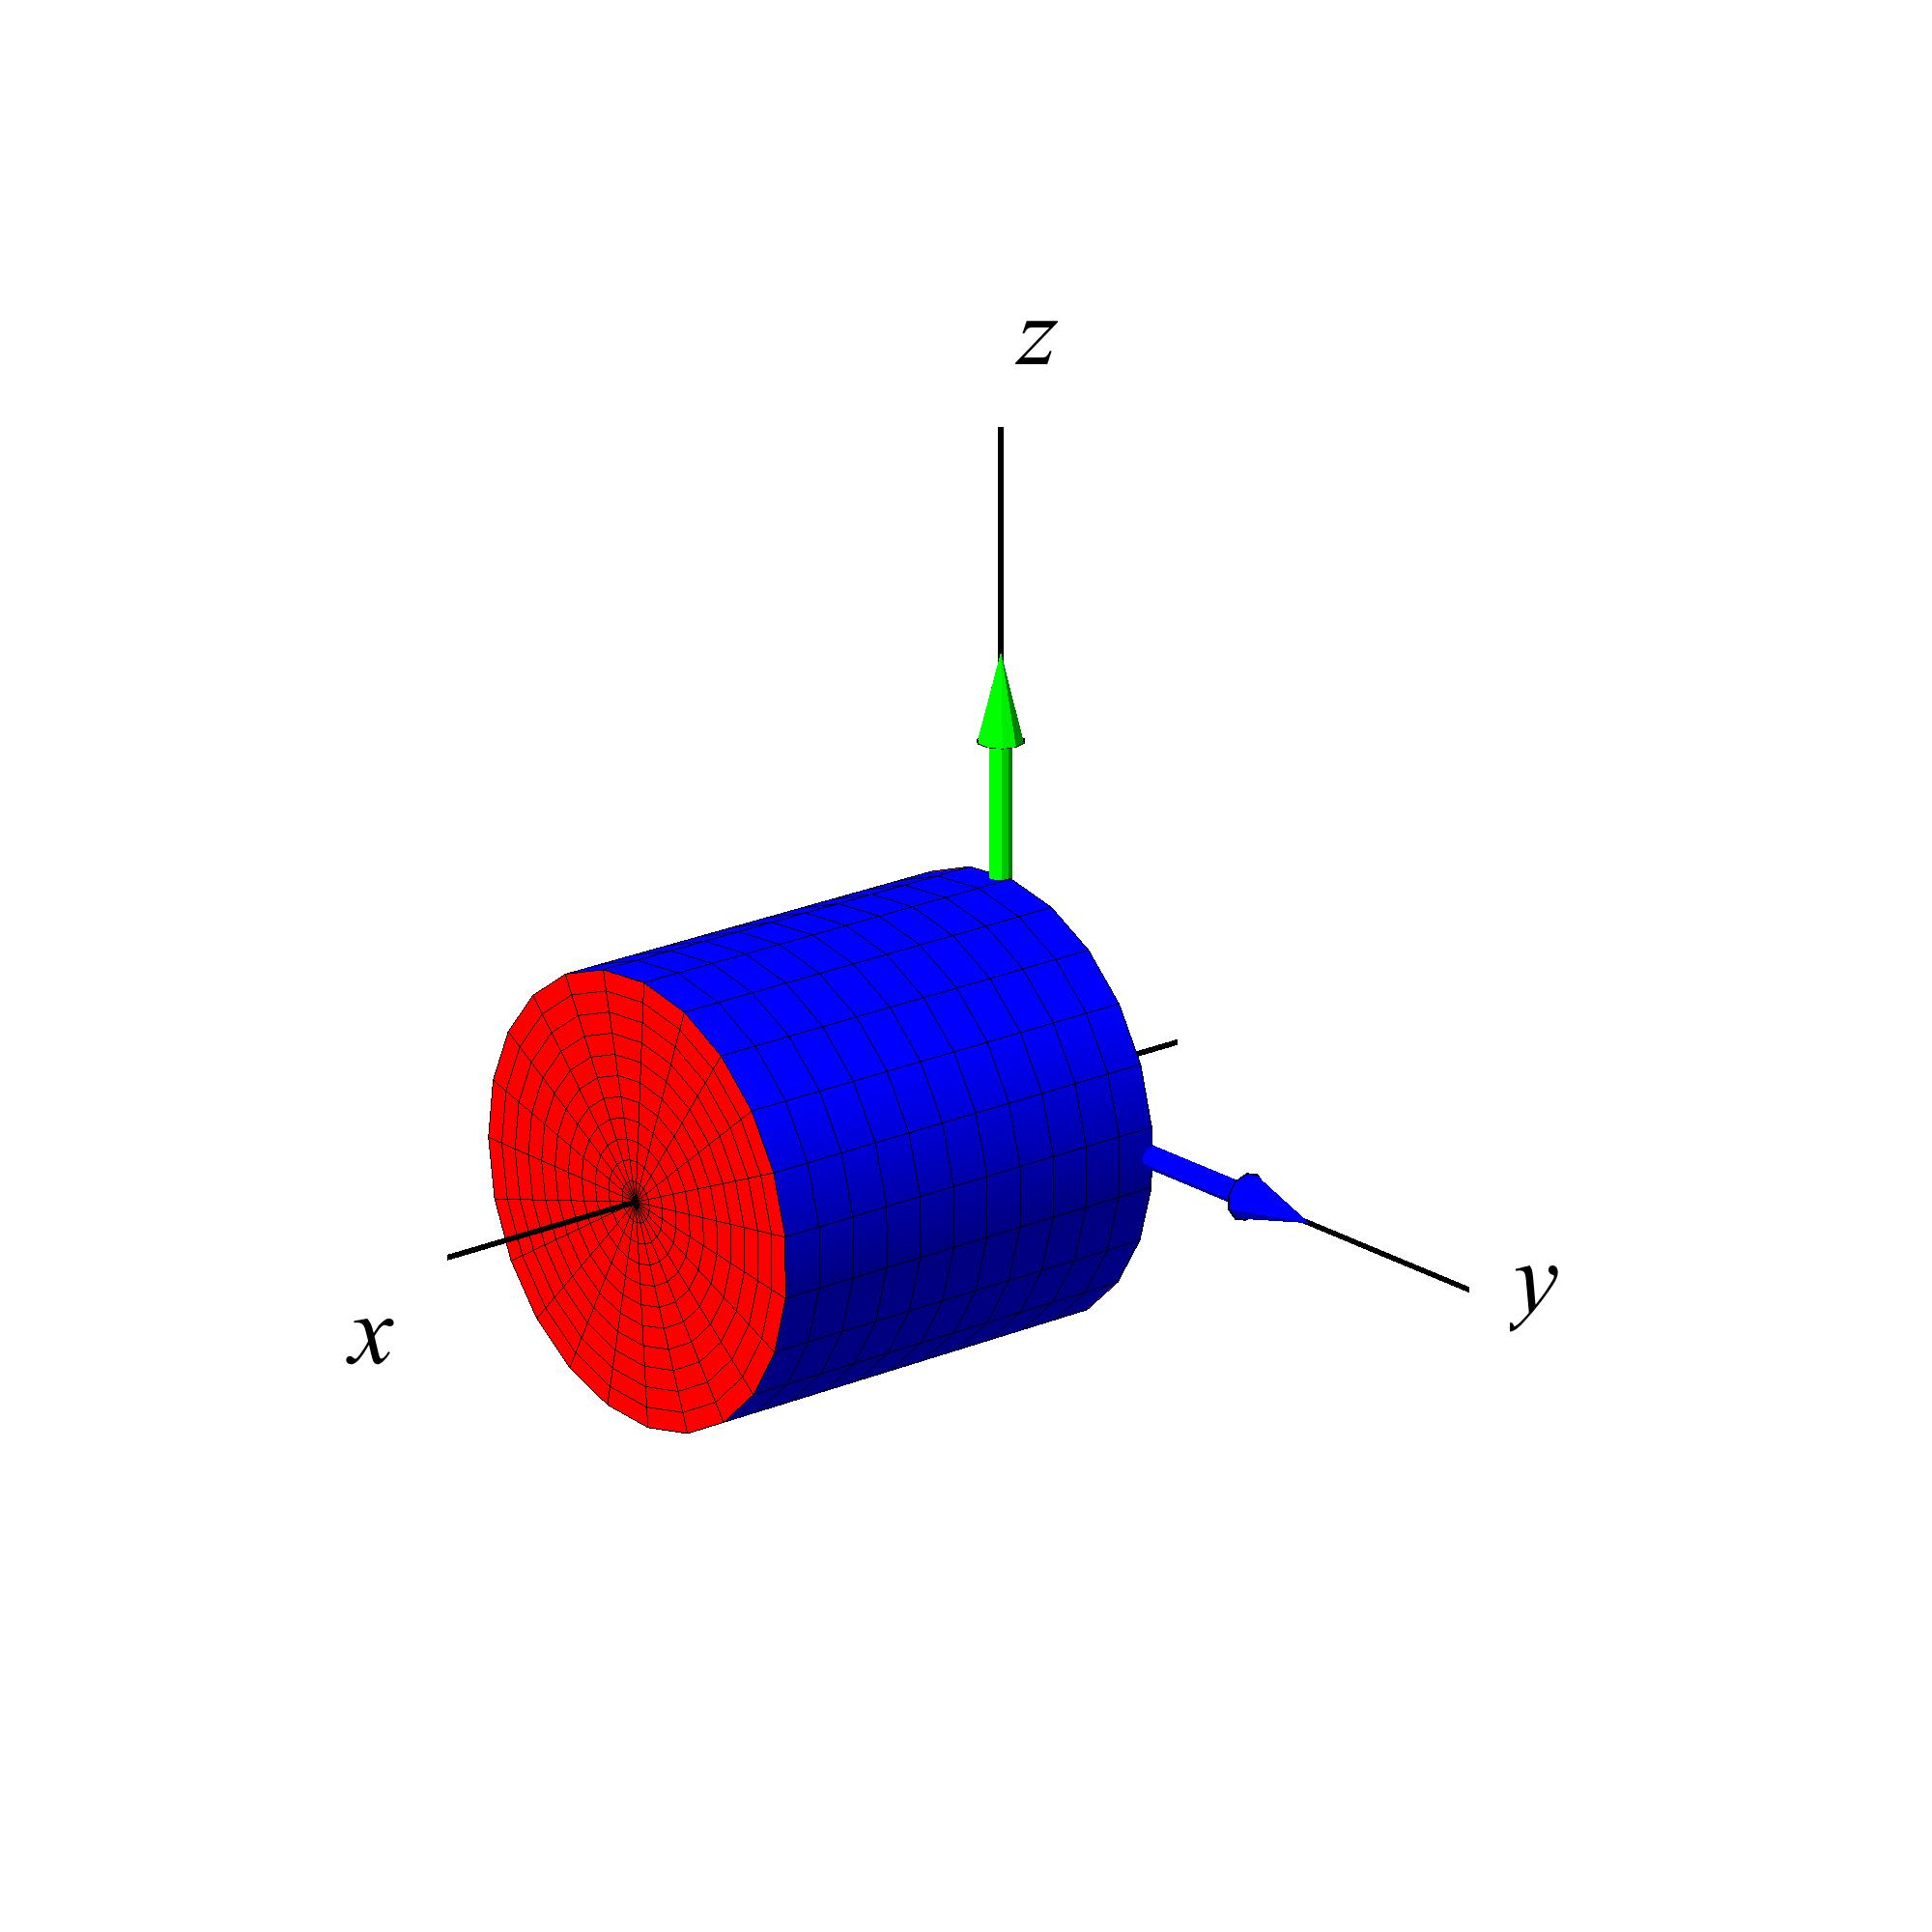
\includegraphics[width=70mm]{FIGS/plotCylFlow1}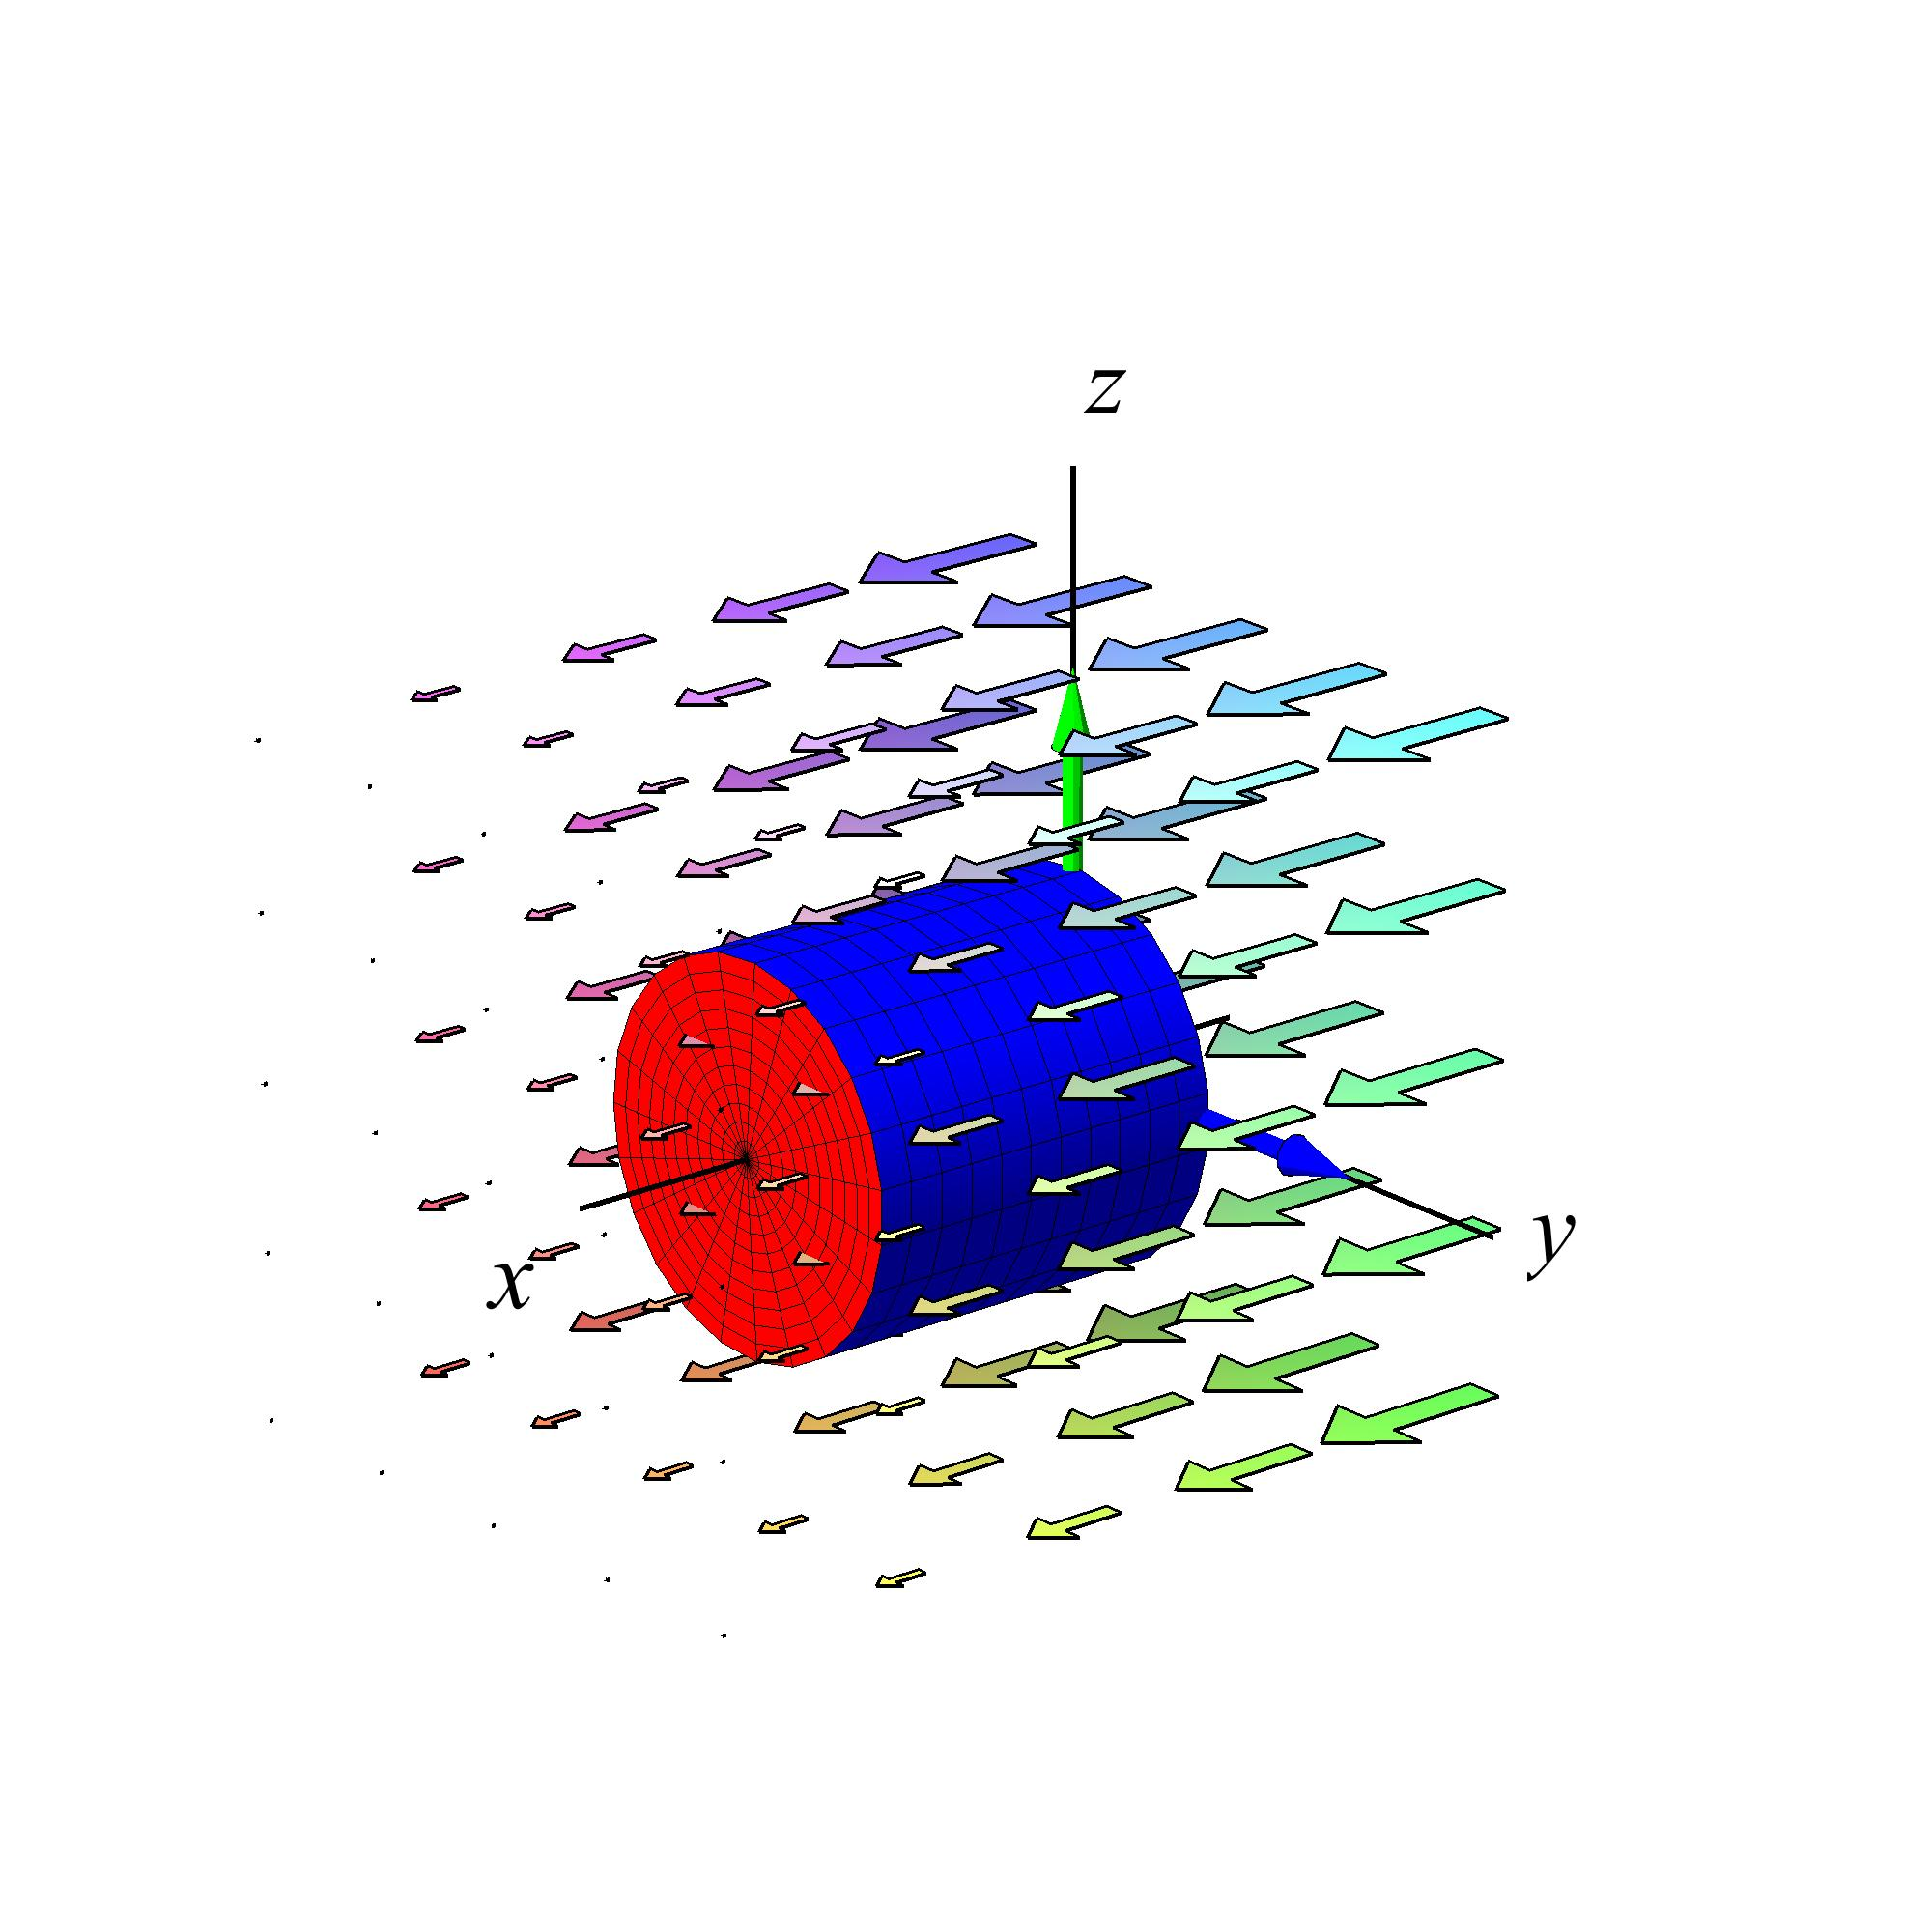
\includegraphics[width=70mm]{FIGS/plotCylFlow2}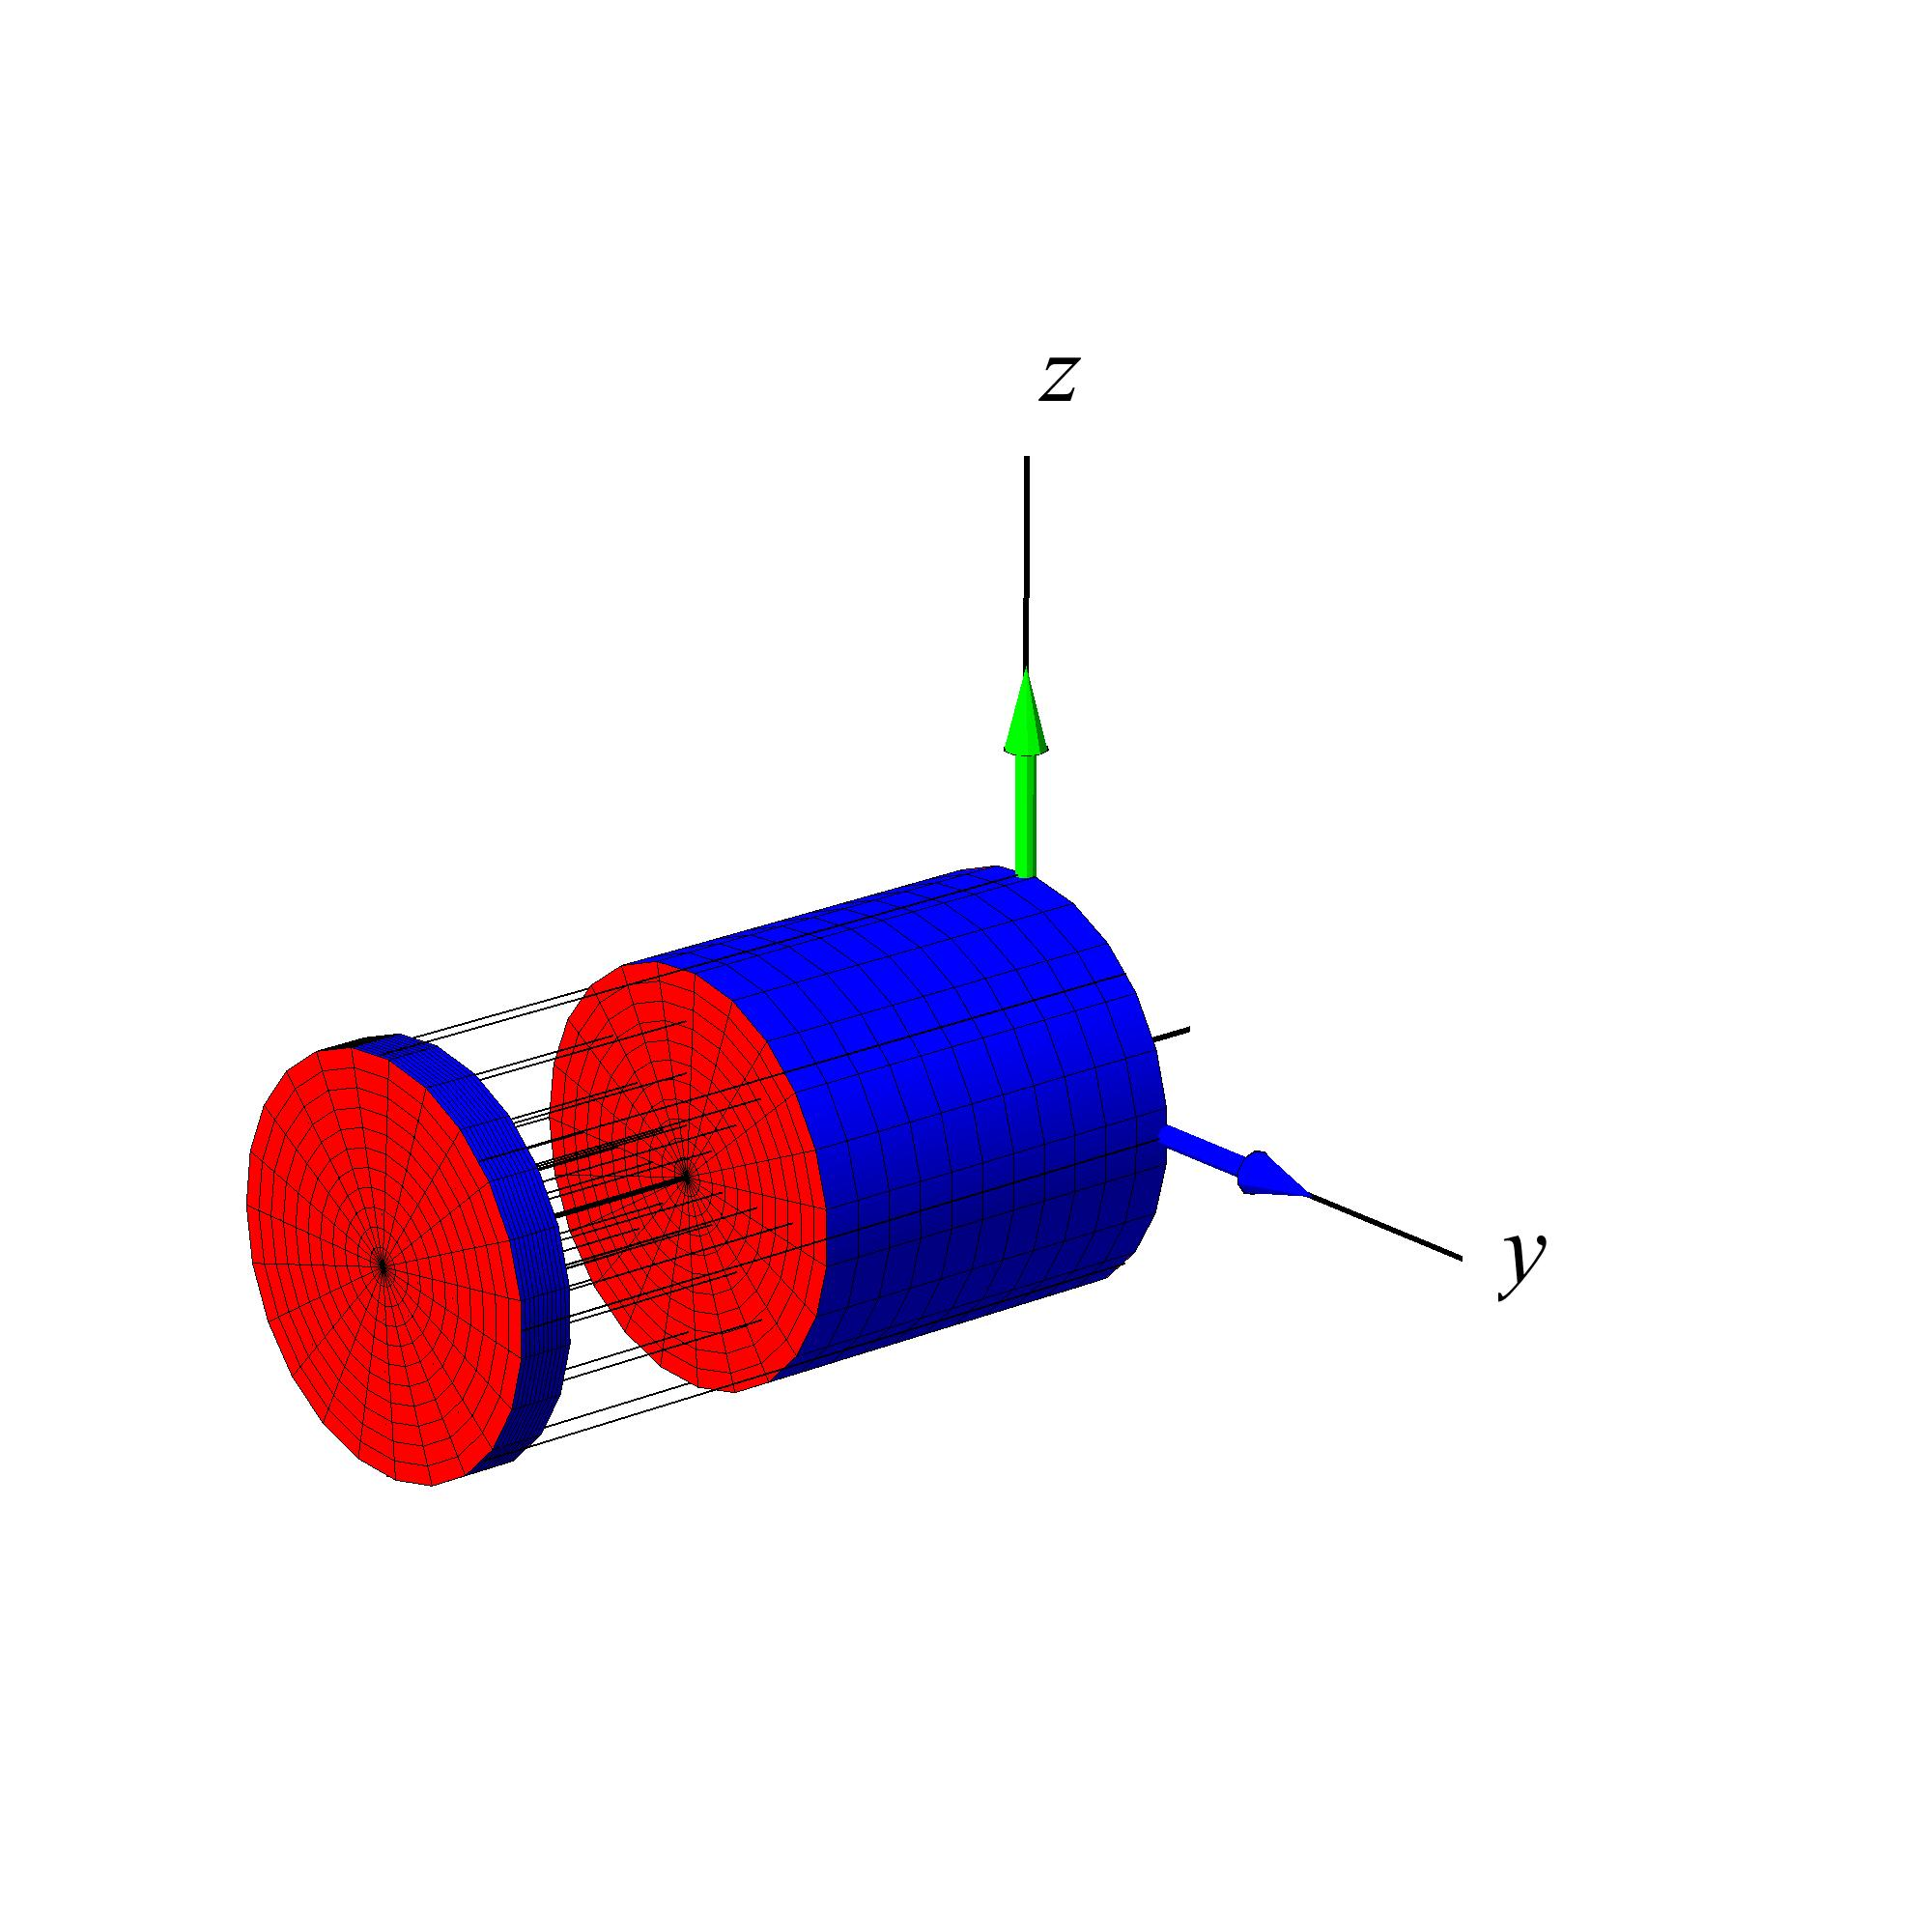
\includegraphics[width=70mm]{FIGS/plotCylFlow3}}
\begin{center}
\caption{\small{Et vektorfelt som er parallelt med $x$-aksen og et billede efter lidt længere tids flow. Efter meget lang tid bliver hele cylinderen mast sammen til en cirkelskive ved $x=2$.
Se eksempel \ref{exampCylFlow}.}} \label{figCylFlow}
\end{center}
\end{figure}

\begin{aha}
Fluxen gennem de to endeskiver på cylinderen i figur \ref{figCylFlow} afhænger af vektorfeltets værdi i disse endpunkter -- se eksempel \ref{exampCylFlow}. Da rumfanget af cylinderen antydes at blive mindre ved flowet giver den inspektion en formodning om, at den totale flux {\emph{ud}} gennem de to endeskiver er negativ. Det er i fuld overensstemmelse med, at vektorfeltet i det viste tilfælde er $\mathbf{V}(x,y,z) = (f(x), 0,0) = (2-x, 0,0)$, som i henhold til beregningen i eksempel \ref{exampCylFlow} giver den totale flux:
\begin{equation}
\Flux(\mathbf{V}, \partial \Omega) = (1 - 2) \cdot \frac{\pi}{4} = - \frac{\pi}{4} \quad .
\end{equation}
Det vil sige at der er større rumfang-deformation \emph{ind i cylinderen} ved $x=0$ end der er rumfang-deformation \emph{ud af} cylinderen ved $x=1$. Den tidsafledede af rumfanget ved flowet er negativ, således at cylinderen netop bliver mindre når alle punkter følger med deres respektive flowkurver. Det gælder faktisk i dette tilfælde ikke bare for små $t$-værdier men for alle $t > 0$, således at cylinderen bliver  helt kollapset og trykket totalt sammen til en flad cirkelskive ved $x=2$ til tiden $t=\infty$ .
\end{aha}


%%%%%%%%%%%%%%%%%%%%%%%%%%%%%%%%%%%%%%%%%%%%%%%%%%%
%%%%%%%%%%%%%%%%%%%%%%%%%%%%%%%%%%%%%%%%%%%%%%%%%%%
%%%%%%%%%%%%%%%%%%%%%%%%%%%%%%%%%%%%%%%%%%%%%%%%%%%
%%%%%%%%%%%%%%%%%%%%%%%%%%%%%%%%%%%%%%%%%%%%%%%%%%%


\section{Motivering af divergensen via flow-ekspansion}
Lad os betragte en massiv kugle $K_{\rho}$ i
rummet med radius $\rho$ og  centrum i $(0,0,0)$
og lad os udvide denne kugle ved at lade alle
punkterne i den flyde med flowkurverne for
eksplosionsvektorfeltet ${\bf{V}}(x,y,z) = (x, y,
z)$. \\

Den massive kugle har parameterfremstillingen:
\begin{equation}
K_{\rho} \quad : \quad \mathbf{r}(u,v,w) = (u\cdot\sin(v)\cdot \cos(w), u\cdot \sin(v)\cdot \sin(w), u\cdot \cos(v)) \quad ,
\end{equation}
hvor  $(u,v,w) \in [0, \rho]\times [0, \pi] \times [-\pi, \pi]$.


Ifølge flow-løsningerne til dette eksplosionsvektorfelt
vokser radius af kuglen
med faktoren $e^{T}$, hvor $T$ er flow-tiden. Det ser vi på følgende måde:\\

De generelle flow-kurver for vektorfeltet findes jo ved at løse differentialligningssystemet:
\begin{equation}
\left[
  \begin{array}{c}
    x'(t) \\
    y'(t) \\
    z'(t) \\
  \end{array}
\right] = (\mathbf{V}(x(t), y(t), z(t)))^{\top} = \left[
                                                    \begin{array}{c}
                                                     x(t) \\
                                                      y(t) \\
                                                      z(t) \\
                                                    \end{array}
                                                  \right] \quad .
\end{equation}
Den generelle løsning er her:
\begin{equation}
\left[
  \begin{array}{c}
    x(t) \\
    y(t) \\
    z(t) \\
  \end{array}
\right]
  = \left[
  \begin{array}{c}
    c_{1} \cdot \e^{t} \\
    c_{2} \cdot \e^{t} \\
     c_{3}\cdot \e^{t} \\
  \end{array}
\right]
\end{equation}
hvor $c_{1}$, $c_{2}$, og $c_{3}$ er arbitrære konstanter.\\

De specielle løsninger, flowkurverne  $ \widetilde{\mathbf{r}}(u,v,w,t)$ igennem kuglepunkterne $(x_{0}, y_{0}, z_{0}) = \mathbf{r}(u,v,w) = (u\cdot\sin(v)\cdot \cos(w), u\cdot \sin(v)\cdot \sin(w), u\cdot \cos(v))$ er så givet ved følgende parametriserede linjer i rummet:
\begin{equation}
\left(\widetilde{\mathbf{r}}(u,v,w,t)\right)^{\top} = \left[
                                           \begin{array}{c}
                                                x_{0}\cdot \e^{t} \\
     y_{0}\cdot \e^{t} \\
     z_{0}\cdot \e^{t} \\
                                           \end{array}
                                         \right] = \left[
                                           \begin{array}{c}
                                              \e^{t}  \cdot (u\cdot\sin(v)\cdot \cos(w)) \\
    \e^{t}  \cdot ( u\cdot \sin(v)\cdot \sin(w))  \\
  \e^{t}  \cdot (u\cdot \cos(v))  \\
                                           \end{array}
                                         \right] \quad .
\end{equation}
Disse linjer og deres parametriseringer giver flow-kurven igennem \emph{ethvert} punkt i den massive kugle.\\


Det rumlige område  $\Omega_{F_{\mathbf{r}}}(t)$ som efter tiden $t$ er \emph{tilføjet} den massive kugle, er dermed allerede parametriseret: Vi skal blot sætte $u = \rho$ i ovenstående flowlinje-para\-me\-tri\-se\-rin\-ger. Det vil sige, vi finder igen ud af, hvordan flowet af kuglens overflade bidrager til volumenforøgelsen (regnet med fortegn):
 \begin{equation}
 \Omega_{F_{\mathbf{r}}}(T) \quad : \quad \widetilde{\mathbf{r}}(\rho,v,w, t) =
 \e^{t}  \cdot \rho \cdot (\cos(v)\cdot \cos(w), \, \sin(v), \, \cos(v)\cdot \sin(w) ) \quad ,
 \end{equation}
hvor $t \in [0, T]$, $v \in [0, \pi]$, og $w \in [-\pi, \pi]$. Det ses, at $\widetilde{\mathbf{r}}(\rho,v,w, T)$ er en parameterfremstilling for den eksploderende kugles overflade efter tiden $T$, og at det er en kugleflade med radius $\e^{T}\cdot \rho$.
Ved at flyde med flowkurverne for eksplosionsvektorfeltet udvider den oprindelige kugle (med radius $\rho$ til tiden $t=0$) sig til en kugle, der har radius $\e^{T}\cdot \rho$ som påstået.

\begin{aha}
Rumfanget af den eksploderende kugle til tiden $T$ er \emph{summen} af de to rumfang $\Vol_{\pm}(\Omega_{F_{\mathbf{r}}}(T))$ og $\Vol(K_{\rho})$. Det førstnævnte rumfang er det med fortegn regnede volumen af det område, som kuglens \emph{overflade} fejer igennem i løbet af tiden $T$.
\end{aha}

Volumenet af kuglen som funktion af
flow-tiden $t$ er dermed givet ved: $\Vol(\Omega_{F_{\mathbf{r}}}(t)) + \Vol(K_{\rho}) = \Vol(t) =
(4\,\pi/3)\,\rho^{3}\,e^{3t}$. Volumenet af
kuglen vokser derfor (til tiden $t=0$) med
differentialkvotienten
\begin{equation}
\frac{d}{dt}\Vol(t)_{|_{t=0}} =
4\,\pi\,\rho^{3} \quad .
\end{equation}

Denne vækst i volumen har vi essentielt fundet ved at holde øje med
udvidelsen af den massive kugles {\em{overflade}}
$\partial K_{\rho}$ når alle kuglens punkter
flyder langs med vektorfeltets flowkurver -- præcis som vi har dyrket i første halvdel af denne eNote.\\

Intuitivt har vi derfra, at hvis skalarproduktet imellem
vektorfeltet ${\bf{V}}$ og den \emph{udadrettede}
enhedsnormalvektor ${\bf{n}}$ et sted på
overfladen er stor, så vil det lokale bidrag til
volumenforøgelse derfra tilsvarende være stor, fordi
overfladen på det sted skubbes hurtigt udad når den flyder med flowkurverne for vektorfeltet.\\

Dette kan selvfølgelig modsvares af at
skalarproduktet andre steder på overfladen er
negativt, således at fladen skubbes ind\-ad på
de steder. \\

Kort sagt ser vi igen, at den totale
udadrettede flux af vektorfeltet igennem
overfladen af det rumlige område giver (den med fortegn regnede) volumenforøgelse.\\

Den tilsvarende udvidelse af sætning \ref{thmFluxVolEkspand} er derfor:


\begin{theorem}[Total flux ud gennem overflade af rumligt område] \label{thmGaussFlux}
Lad $\Omega_{\bf{r}}$ betegne et vilkårligt parametriseret område i
rummet med {\em{udadrettet}} enhedsnormalvektorfelt $\,
{\bf{n}}_{\partial \Omega}\, $ langs overfladen $\,\partial
\Omega_{\bf{r}}\,$.\\

Overfladen kan gerne være sammensat af glatte parametriserede fladestykker som f.eks. overfladen på et polyeder.\\

 Lad $\,{\bf{V}}(x,y,z)\,$ betegne et vilkårligt glat
vektorfelt i rummet. \\

Vi lader alle punkterne i $\,\Omega_{\bf{r}}\,$
flyde tiden $\,t\,$ langs flowkurverne for vektorfeltet
$\,{\bf{V}}(x,y,z)\,$. \\

Det med fortegn (i forhold til ${\bf{n}}_{\partial \Omega}$) regnede volumen $\,\Vol_{\pm}(t)\,$ af området efter
denne deformation har da følgende differentialkvotient til tiden
$\,t = 0\,$:
\begin{equation} \label{eqnGaussFlux}
\frac{d}{dt}\Vol_{\pm}(t)_{|_{t=0}} \, = \, \int_{\partial
\Omega_{\bf{r}}}{\bf V}\cdot {\bf n}_{\partial \Omega}\,d\mu \, = \,
\Flux({\bf{V}},
\partial \Omega_{\bf{r}}) \quad .
\end{equation}
\end{theorem}

\begin{example}[Eksplosion af massiv kugle] \label{exampExplodeKugle}
Vi checker sætningen i det konkrete tilfælde med
den eksploderende kugle: Fluxen af
eksplosionsvektorfeltet ud igennem kuglens
overflade er simpelthen overfladens areal
$4\,\pi\,\rho^{2}$ gange skalarproduktet ${\bf
V}\cdot {\bf n}$, fordi dette skalarprodukt i dette
specielle tilfælde er konstant: ${\bf V}\cdot
{\bf n} = \Vert{\bf{V}}\Vert = \sqrt{x^2 + y^2 +
z^2} = \rho\,\,$. Derfor er den totale flux
$4\,\pi\,\rho^{3}$, altså præcis
differentialkvotienten (til tiden $t=0$) af
volumenet som funktion af flowtiden
$\,t\,$. Vi har således verificeret sætningen i
dette specielle eksempel.
\end{example}

\begin{think}
De parametriserede rumlige områder, vi betragter,
har jo sædvanligvis en rand, der består af $6$
sideflader. Det betyder, at beregningen af
volumenvæksten af området ved deformationen langs
flowkurverne kræver beregning af $6$ udadrettede
flux-bidrag -- eet bidrag for hver sideflade.\\

Hvis to af de $6$ sideflader ved en standardparametrisering af et rumligt område
er sammenfaldende eller delvis sammenfaldende,
så vil standard enheds-normalerne for den ene sideflade være præcis modsatrettet
standard enheds-normalerne for den anden sideflade der hvor sidefladerne er sammenfaldende, således at
de tilsvarende fluxbidrag der vil \emph{ophæve hinanden}!
\end{think}




For et vilkårligt glat vektorfelt i rummet kan vi
undersøge volumenforøgelsen (ved flow langs
vektorfeltets flowkurver) for en lille massiv
kugle $K_{\rho}$, der har centrum i et givet
punkt, f.eks. $p = (x_{0}, y_{0}, z_{0})$ og
radius $\rho$. Vi Taylor-udvikler vektorfeltets
koordinatfunktioner $V_{1}$, $V_{2}$ og $V_{3}$,
til 1. orden med udviklingspunkt $(x_{0}, y_{0},
z_{0})$ og finder den udadrettede flux af
vektorfeltet igennem den lille kug\-les overflade
$\partial K_{\rho}$. Denne flux divideret med
volumenet $(4\,\pi/3)\,\rho^{3}$ af den massive
kugle $K_{\rho}$ har en grænseværdi når radius
$\rho$ går imod $0$. Se skitsen til den beregning
nedenfor.\\

Det viser sig (se nedenfor) at denne grænseværdi
netop er \emph{divergensen af vektorfeltet} i det
betragtede punkt! I lyset af sætning
\ref{thmGaussFlux} og ligning
(\ref{eqnGaussFlux}) har vi derfor motivereret
følgende tolkning af divergensen:

\begin{theorem} \label{thmDivGeom}
Divergensen af et vektorfelt udtrykker {\em{den
{volumen-relative lokale flux} ud gennem
overfladen}} for vektorfeltet og dermed også
{\em{den relative lokale volumen-vækst}} ved
deformation langs flowkurverne for vektorfeltet:
\begin{equation}
\begin{aligned}
\Div({\bf{V}})(x_{0}, y_{0}, z_{0})
&= \, \lim_{\rho \to 0}\left(
\frac{1}{\Vol(K_{\rho})}\Flux({\bf{V}},
\partial K_{\rho})\right) \,\\
 &= \,
\lim_{\rho \to 0}\left( \frac{1}{\Vol(K_{\rho})}
\frac{d}{dt}\Vol_{\pm}(t)_{|_{t=0}}    \right)
 \quad .
\end{aligned}
\end{equation}
\end{theorem}

\begin{bevis}
Vi vil kun skitsere, hvordan divergensen fremkommer ved den
antydede fremgangsmåde. Vi simplificerer
fremstillingen på to måder: Dels vil vi vælge et
koordinatsystem så $p = (0,0,0)$, og dels vil vi
kun medtage lineariseringen af ${\bf{V}}(x,y,z)$
omkring $(0,0,0)$ ($\varepsilon$-leddene fra
Taylors grænseformler for de 3 koordinatfunktioner
tages altså ikke med). (Til gengæld er
beregningerne helt eksakte for vektorfelter af
højest første grad.)\\

Opgaven er altså at genfinde $\,\Div({\bf{V}})$ i
punktet $(0,0,0)$ ved hjælp af en fluxberegning.
Vi be\-gyn\-der med at bruge Taylors grænseformel på
$\,{\bf{V}}(x,y,z)\,$. Det underforstås, at
$V_{i}$ og de partielle afledede af $V_{i}$
evalueres i udviklingspunktet $(0,0,0)$ medmindre
andet antydes.


\begin{equation}
\begin{aligned}
{\bf{V}}(x,y,z) = (\, & V_{1} + x\,\frac{\partial V_{1}}{\partial x}
 + y\,\frac{\partial V_{1}}{\partial y}
 + z\,\frac{\partial V_{1}}{\partial z},\\
& V_{2} + x\,\frac{\partial V_{2}}{\partial x}
 + y\,\frac{\partial V_{2}}{\partial y}
 + z\,\frac{\partial V_{2}}{\partial z},\\
 & V_{3} + x\,\frac{\partial V_{3}}{\partial x}
 + y\,\frac{\partial V_{3}}{\partial y}
 + z\,\frac{\partial V_{3}}{\partial z} \,) \quad .
\end{aligned}
\end{equation}

Idet enhedsnormalvektorfeltet på overfladen af
den lille massive $\rho$-kugle $K_{\rho}$ med
centrum $(0,0,0)$ er givet ved $\,{\bf{n}} =
(x/\rho,\, y/\rho,\, z/\rho)\,$ følger det, at
integranden i fluxberegningen er følgende:

\begin{equation} \label{eqVolFlux}
\begin{aligned}
{\bf{V}}(x,y,z)\cdot {\bf{n}} = \left( \frac{1}{\rho}\right)(\, &
x\,V_{1} + x^{2}\,\frac{\partial V_{1}}{\partial x}
 + xy\,\frac{\partial V_{1}}{\partial y}
 + xz\,\frac{\partial V_{1}}{\partial z} + \\
& y\,V_{2} + yx\,\frac{\partial V_{2}}{\partial x}
 + y^{2}\,\frac{\partial V_{2}}{\partial y}
 + yz\,\frac{\partial V_{2}}{\partial z} + \\
 & z\,V_{3} + zx\,\frac{\partial V_{3}}{\partial x}
 + zy\,\frac{\partial V_{3}}{\partial y}
 + z^{2}\,\frac{\partial V_{3}}{\partial z}\, ) \quad .
\end{aligned}
\end{equation}

Tilbage er nu kun at integrere dette udtryk over
kuglens overflade $\partial K_{\rho}$ og dernæst
dividere med kuglens volumen $\Vol(K_{\rho})$.
Selv om det nok kan se kompliceret ud, så er det
faktisk rimelig simpelt i betragtning af følgende
identiteter:

\begin{equation} \label{eqKugleintegraler}
\begin{aligned}
&\int_{\partial K_{\rho}}\,x \,\,d\mu \, = \,
\int_{\partial K_{\rho}}\,y \,\,d\mu \, = \,
\int_{\partial K_{\rho}}\,z \,\,d\mu \, = \,0 \quad , \\
&\int_{\partial K_{\rho}}\,x^{2}\,\, d\mu \, = \,
\int_{\partial K_{\rho}}\,y^{2}\,\, d\mu \, = \,
\int_{\partial K_{\rho}}\,z^{2}\,\, d\mu \, = \, (4\,\pi/3)\,\rho^{4}\, = \, \rho\,\Vol(K_{\rho})\quad , \\
& \int_{\partial K_{\rho}}\,x\,y \,\,d\mu \, = \,
\int_{\partial K_{\rho}}\,x\,z \,\,d\mu \, =
\,\int_{\partial K_{\rho}}\,z\,y \,\,d\mu \, =
\,0 \quad .
\end{aligned}
\end{equation}



Fra ligning (\ref{eqKugleintegraler}) følger nu
f.eks. følgende bidrag til integralet over
kuglefladen $\partial K_{\rho}$ af
høj\-re\-si\-den i ligning (\ref{eqVolFlux}).
(Bemærk, at $\frac{\partial V_{1}}{\partial
x}(0,0,0)$ er en konstant, der kan sættes udenfor
integraltegnet.):
\begin{equation}
\int_{\partial
K_{\rho}}\,\left(\frac{1}{\rho}\right)\,x^{2}\,\,\frac{\partial
V_{1}}{\partial x}(0,0,0)\,\, d\mu \, = \,
\Vol(K_{\rho})\,\frac{\partial V_{1}}{\partial
x}(0,0,0) \quad .
\end{equation}

Ialt fås naturligvis 3 sådanne bidrag til
integralet over kuglefladen $\partial K_{\rho}$
af høj\-re\-si\-den i ligning (\ref{eqVolFlux}),
og da integralet over $\partial K_{\rho}$
 af venstresiden i ligning (\ref{eqVolFlux}) netop er fluxen $\Flux({\bf{V}},
 \partial K_{\rho})$ har vi derfor følgende
 identitet i dette simplificerede tilfælde:
\begin{equation} \label{eqLimitDiv}
\begin{aligned}
\frac{1}{\Vol(K_{\rho})}\Flux({\bf{V}}, \partial K_{\rho})
\, &= \,
\frac{1}{\Vol(K_{\rho})}\int_{\partial K_{\rho}}\,{\bf{V}}\cdot
{\bf{n}} \,\,d\mu \, \\
&= \, \frac{\partial V_{1}}{\partial x}(0,0,0) +
\frac{\partial V_{2}}{\partial y}(0,0,0) +
\frac{\partial V_{3}}{\partial z}(0,0,0) \, \\ &
= \, \Div({\bf{V}})(0,0,0) \quad .
\end{aligned}
\end{equation}


For generelle vektorfelter gælder den tilsvarende
identitet kun i den grænse, hvor $\rho$ er meget
lille (altså for $\rho \to 0$), således at
ovenstående brug af Taylor's grænseformel for $\mathbf{V}(x,y,z)$ til
første orden netop bliver den dominerende
repræsentant for vektorfeltet indenfor kuglen
$K_{\rho}$. For vektorfelter af højest første
grad gælder identiteten (\ref{eqLimitDiv}) dog
som nævnt for alle værdier af $\rho$. Det skyldes
naturligvis, at uanset radius $\rho$ er
vektorfeltet jo i det specielle tilfælde eksakt
repræsenteret i hele $K_{\rho}$ ved sin
Taylors grænseformel til første orden med
udviklingspunkt i centrum.\\

Hermed har vi afsluttet skitseringen af beviset
for den lokale bestemmelse af divergensen af et
vektorfelt og vist den geometriske tolkning i
sætning \ref{thmDivGeom}.
\end{bevis}




\begin{exercise}
Vis de ovenstående identiteter i ligning
(\ref{eqKugleintegraler}). I de tilfælde hvor
integralet er $0$ kan dette vises ved en
fortegns- og symmetribetragtning.
\end{exercise}




Denne fremstilling af divergensen åbner nu op for
en naturlig ide, som går i den modsatte retning:\\

Da den lokale punktvise volumen-vækst ved
deformation af et rumligt område langs
flowkurverne for et givet vektorfelt er bestemt
af divergensen af vektorfeltet, så er følgende en
rimelig formodning: Hvis vi integrerer
divergensen over et område i rummet, så skulle
resultatet gerne være sammenlignelig med den
totale volumenvækst af hele området. Altså groft
sagt skulle summen af de lokale volumentilvækster
gerne være den totale volumentilvækst. \\

 Dette er
præcis indholdet af Gauss' sætning, som vi nu
formulerer i kombination med Sætning
\ref{thmGaussFlux}:



%%%%%%%%%%%%%%%%%%%%%%%%%%%%%%%%%%%%%%%%%%%%%%%%%%%%%%%%%%%%%%%%%%
%%%%%%%%%%%%%%%%%%%%%%%%%%%%%%%%%%%%%%%%%%%%%%%%%%%%%%%%%%%%%%%%%%
%%%%%%%%%%%%%%%%%%%%%%%%%%%%%%%%%%%%%%%%%%%%%%%%%%%%%%%%%%%%%%%%%%

\section{Gauss' divergens-sætning} \label{secGauss}



\begin{figure}[h]
\centerline{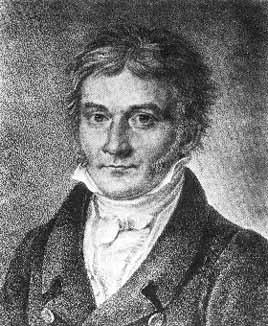
\includegraphics[height=60mm]{FIGS/PERSGauss_1828}}
\begin{center}
\caption{\small{Carl Friedrich Gauss.
Se \href{http://www-history.mcs.st-and.ac.uk/Mathematicians/Gauss.html}{Biografi}.}} \label{figGauss}
\end{center}
\end{figure}



\begin{theorem}[{Gauss' divergens-sætning}] \label{thmGauss}
Lad $\,\Omega_{\bf{r}}\,$ betegne et rumligt område med
randoverflade $\,\partial \Omega_{\bf{r}}\,$ og \emph{udadrettet}
en\-heds\-nor\-mal\-vektorfelt $\,{\bf{n}}_{\partial \Omega}\,$ på
rand\-over\-fladen. For ethvert glat vektorfelt $\, {\bf{V}}$ i rummet
gælder så følgende:
\begin{equation} \label{eqGauss}
\frac{d}{dt}\Vol_{\pm}(t)_{|_{t=0}}\, = \,
\int_{\Omega_{\bf{r}}} \, \Div({\bf{V}}) \,\,
d\mu \, = \, \int_{\partial \Omega_{\bf{r}}}{\bf
V} \bm{\cdot} {\bf{n}}_{\partial \Omega}\,\,d\mu \, =
\, \Flux({\bf{V}},
\partial \Omega_{\bf{r}}) \quad ,
\end{equation}
hvor fluxen altså skal beregnes med hensyn til det \emph{udadrettede}
enhedsnormalvektorfelt på rand\-over\-fla\-den af det givne rumlige
område.
\end{theorem}

Begge
sider af følgende lig\-ning, der er essensen af
Gauss' sætning, kan jo beregnes i konkrete tilfælde og dermed
verificere Gauss' sætning:
\begin{equation} \label{eqGaussPure}
\int_{\Omega_{\bf{r}}} \, \Div({\bf{V}}) \,\,
d\mu \, = \, \Flux({\bf{V}},
\partial \Omega_{\bf{r}}) \quad .
\end{equation}

Vi vil her gennemgå nogle eksempler på sådanne dobbelt-beregninger.

\begin{think}
I visse tilfælde er det meget simplere at udregne divergens-integralet over et givet rumligt område
end at udregne fluxen  af vektorfeltet gennem områdets totale overflade.
Hvis man skal udregne sidstnævnte vil man selvfølgelig i stedet bare udregne førstnævnte integral og henvise til
Gauss' divergenssætning. Omvendt er der tilfælde hvor fluxintegralet er simplest at beregne -- så benyttes selvfølgelig tilsvarende duale  strategi.
\end{think}





\begin{example}
Hvis vektorfeltet ${\bf{V}}$ har divergensen $0$
i alle punkter i rummet, så vil ethvert rumligt
område, der flyder med vektorfeltet, bevare sit
volumen. Formen kan naturligvis ændres meget som
tiden går, men volumenet er konstant. Desuden er
fluxen {\em{ud}} igennem overfladen af ethvert
{\em{fastholdt}} rumligt område tilsvarende $0$.
\end{example}



\begin{example} \label{exDivFluxExplosion}
For eksplosionsvektorfeltet ${\bf{V}}(x,y,z) = (x,y,z)$, der har
den konstante divergens $\Div({\bf{V}}) \, = \, 3\,$, gælder altså
følgende for et vilkårligt rumligt område: $ \, 3\,\Vol(\Omega) \, =
\, \Flux({\bf{V}}, \, \partial \Omega)\, $.
\end{example}



\begin{exercise}
Vis (ved direkte udregninger) påstanden om
${\bf{V}}(x,y,z) = (x,y,z)$ i ovenstående eksempel
\ref{exDivFluxExplosion} for det rumlige område, der består af den
massive cylinder i figur \ref{figCylFlow}.
\end{exercise}




\begin{figure}[ht]
\centerline{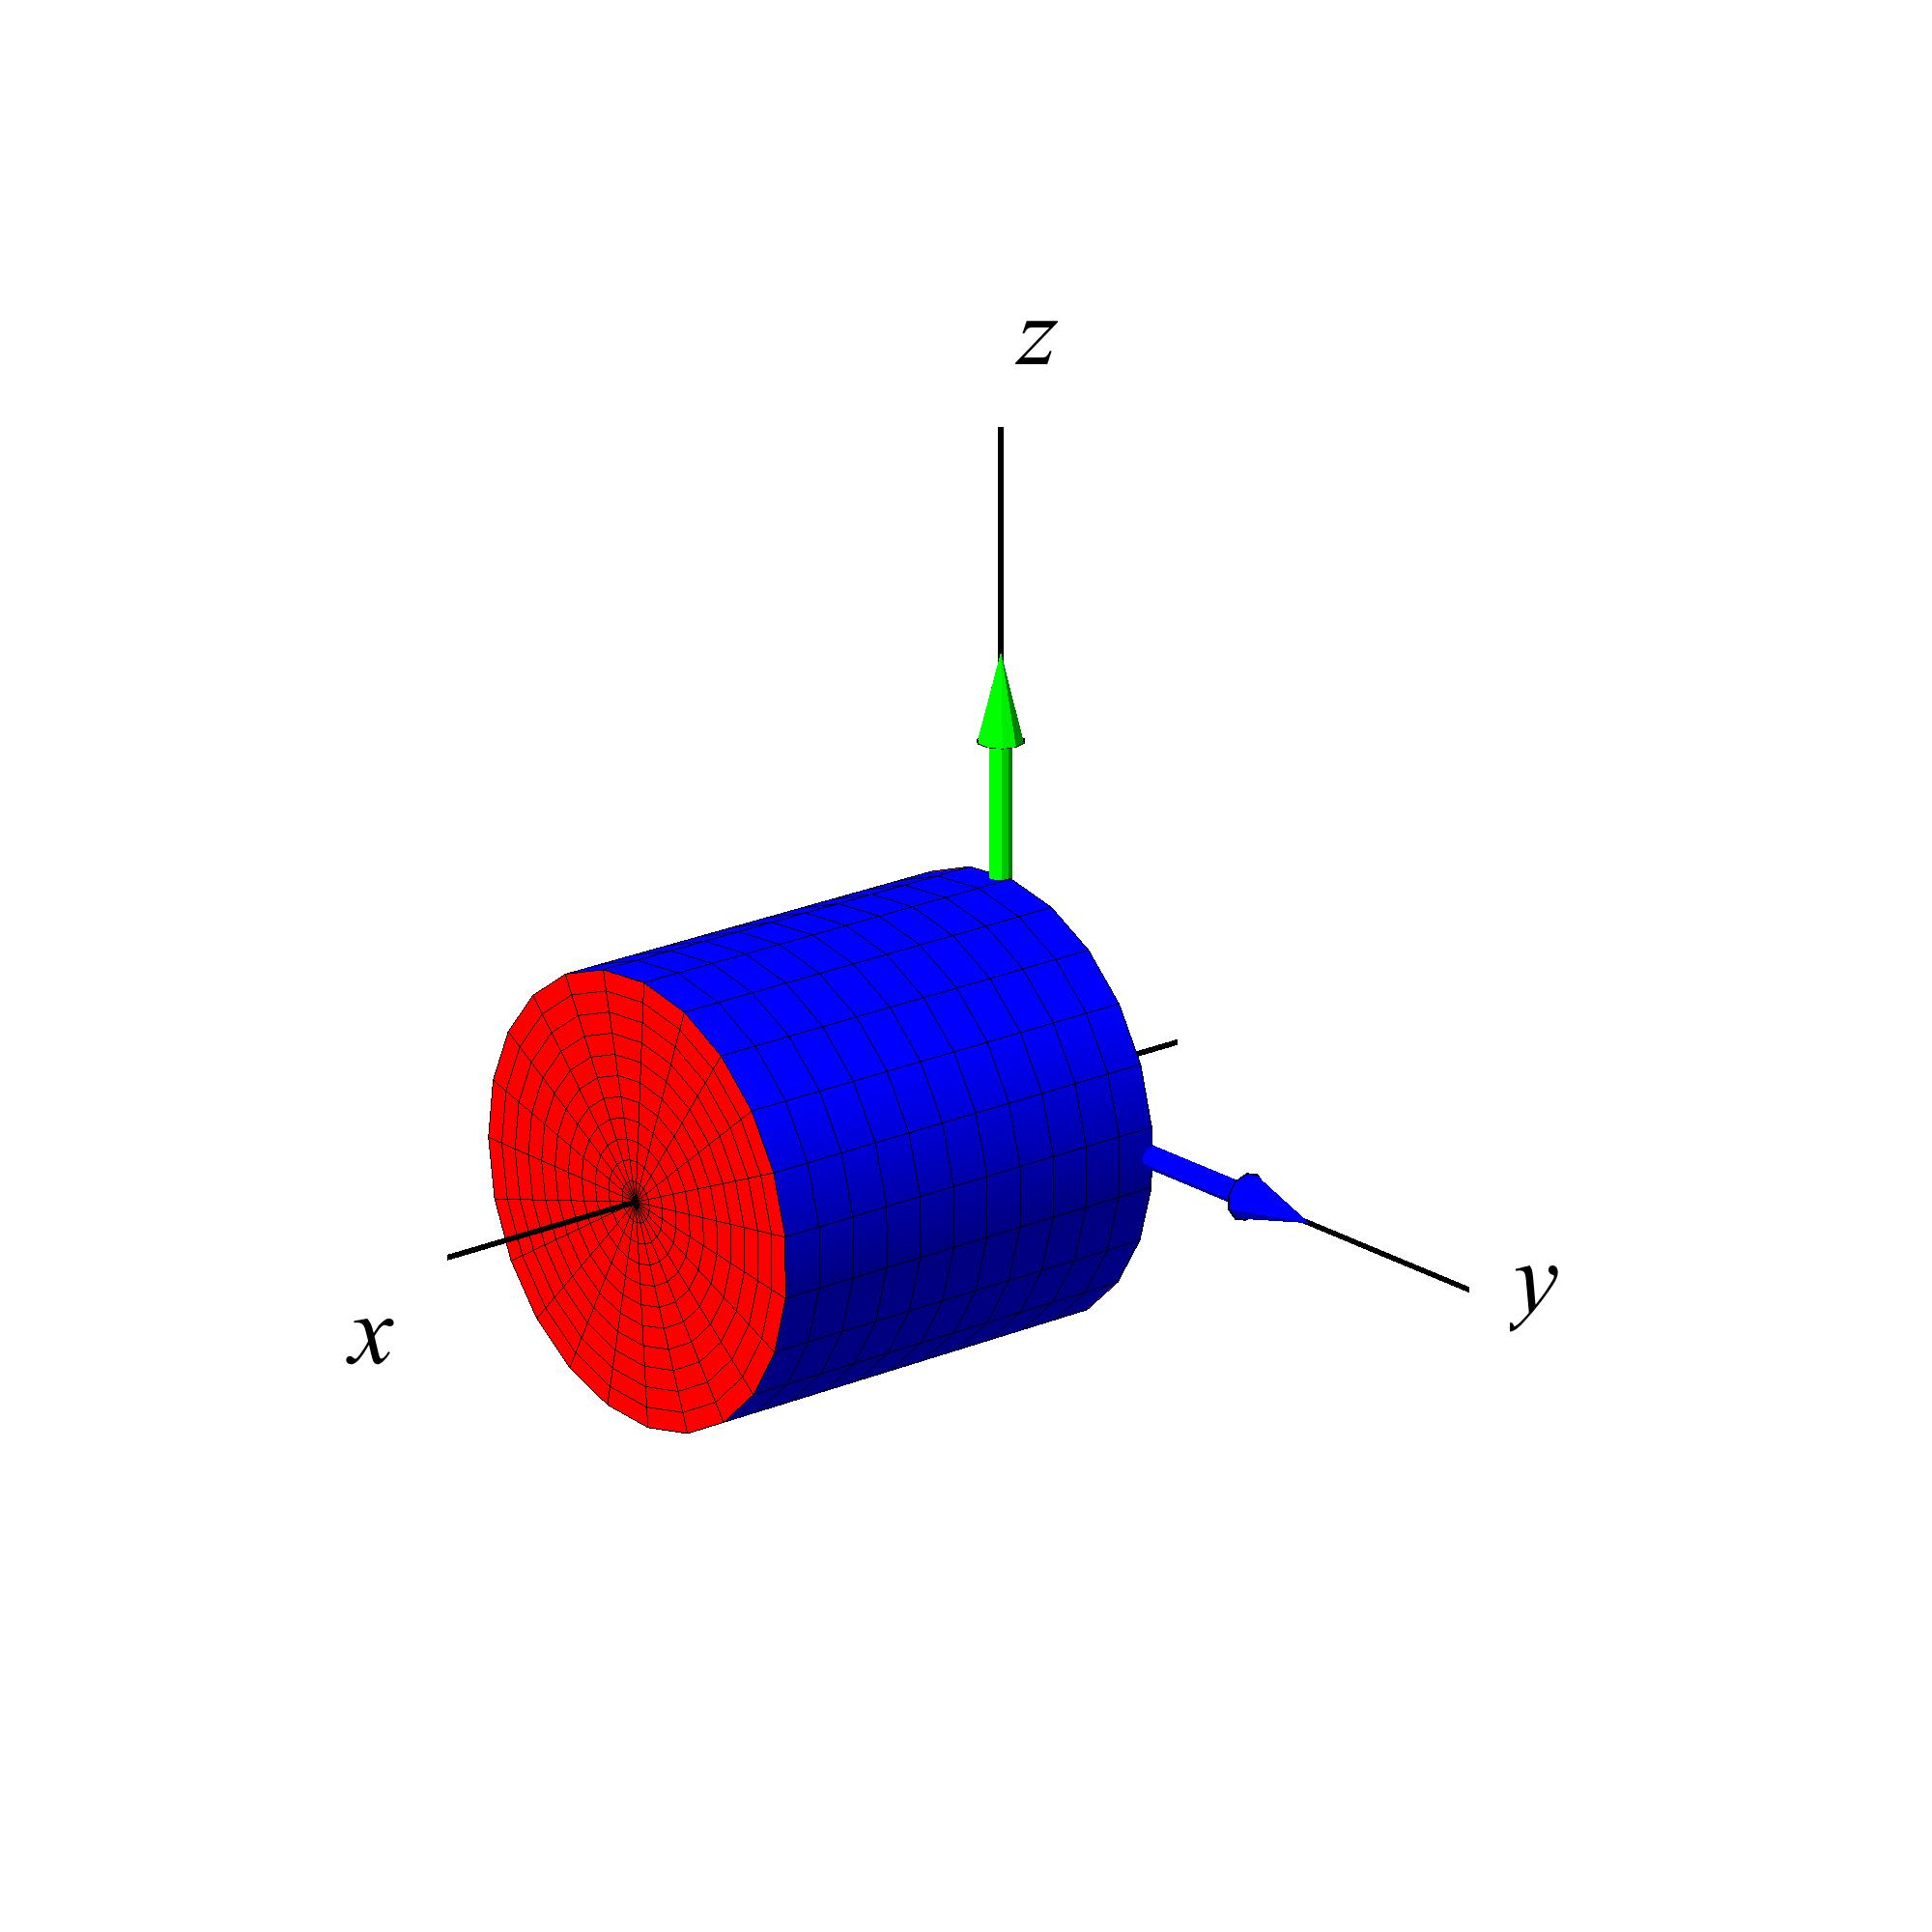
\includegraphics[width=70mm]{FIGS/plotCylFlow1}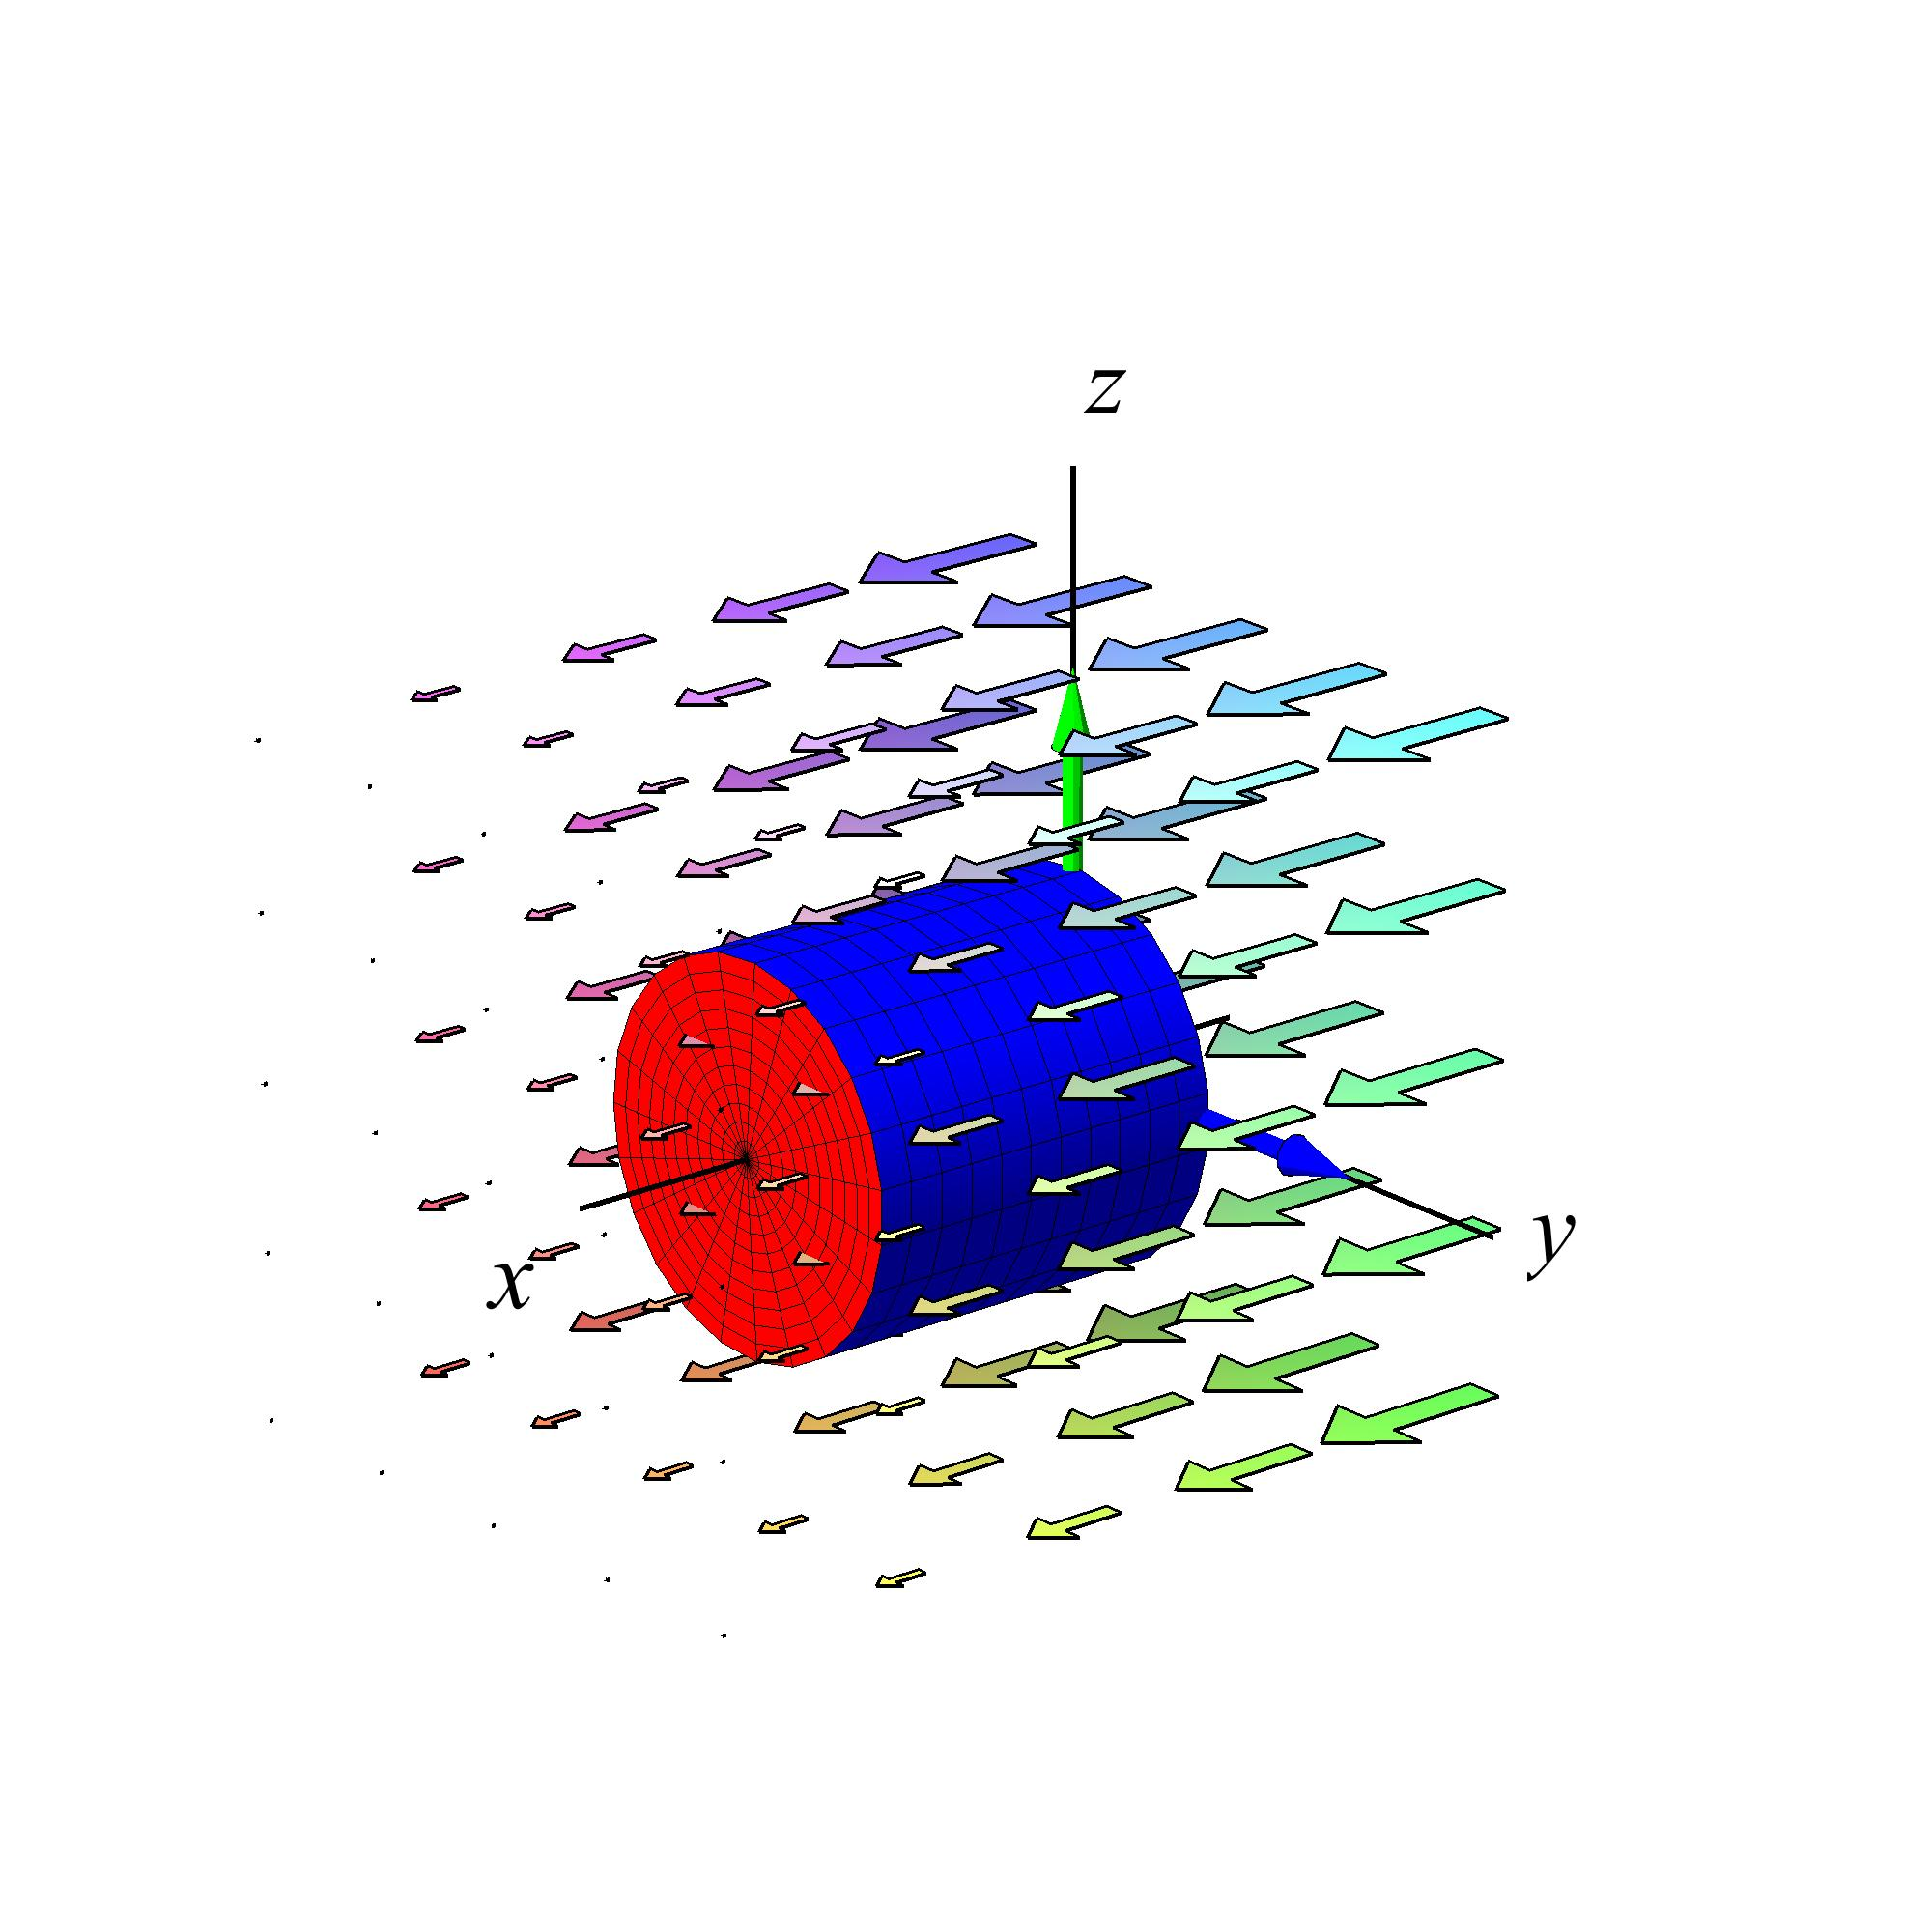
\includegraphics[width=70mm]{FIGS/plotCylFlow2}}
\begin{center}
\caption{\small{Et vektorfelt som er parallelt med $x$-aksen og cylinderen fra eksempel \ref{exampCylFlow}.}} \label{figCylFlow2}
\end{center}
\end{figure}





\begin{example}[Divergensen og fluxen i cylinder-eksemplet]\label{exampCylGauss}
Vi vil illustrere Gauss' sætning for vektorfeltet
\begin{equation}
\mathbf{V}(x,y,z)= (f(x), 0,0) \quad , \quad (x,y,z) \in \mathbb{R}^{3} \quad,
\end{equation}
hvor $f(x)$ er en glat funktion af $x$, idet vi vil beregne integralet af divergensen af vektorfeltet over den massive cylinder med radius $1/2$, $x$-aksen som symmetriakse, og $x$-interval $x \in [0, 1]$, som vi studerede i eksempel \ref{exampCylFlow}. I det eksempel fandt vi den totale flux af vektorfeltet ud gennem cylinderens overflade:
\begin{equation}
\Flux(\mathbf{V}, \partial \Omega) = (f(1) - f(0)) \cdot \frac{\pi}{4} \quad .
\end{equation}
Den totale divergens af vektorfeltet i den massive cylinder er lige så let at beregne:
Den lokale divergens af $\mathbf{V}(x,y,z) = (f(x), 0, 0)$ er i et vilkårligt punkt $(x,y,z)$:
\begin{equation}
\Div(\mathbf{V})(x,y,z) = f'(x) \quad .
\end{equation}
Den massive cylinder har en parameterfremstilling:
\begin{equation}
\Omega_{\mathbf{r}} \quad : \quad \mathbf{r}(u,v,w) = (w, u\cdot \cos(v), u\cdot \sin(v)) \quad ,
\end{equation}
hvor $(u,v,w) \in [0,1/2]\times [-\pi, \pi] \times [0, 1]$.
Jacobifunktionen for parametriseringen er så
\begin{equation}
\Jac_{\mathbf{r}}(u,v,w) = u \quad ,
\end{equation}
således at den totale divergens af vektorfeltet er
\begin{equation}
\begin{aligned}
\int_{\Omega_{\bf{r}}} \, \Div({\bf{V}}) \,\,
d\mu \, &= \, \int_{0}^{1} \int_{-\pi}^{\pi} \int_{0}^{1/2} f'(w) \cdot u \,\, du\,dv\,dw \\
&= \, \int_{0}^{1} \int_{-\pi}^{\pi} \frac{1}{8}\cdot f'(w) \,\,dv\,dw \\
&=  \frac{1}{8}\cdot \int_{0}^{1} 2\cdot \pi \cdot f'(w) \,\,dw \\
&=  \frac{\pi}{4}\cdot \int_{0}^{1} f'(w) \,\,dw \\
&=  \frac{\pi}{4}\cdot \left[f(w) \right]_{w=0}^{w=1} \\
&= (f(1) - f(0)) \cdot \frac{\pi}{4} \quad ,
\end{aligned}
\end{equation}
altså præcis samme resultat som ved flux-beregningen.
\end{example}


\begin{example}[Vektorfelt igennem en kantet torus]\label{exampTorusGauss}
Vi betragter en delmængde af en massive kugle med radius $1/2$, se figur \ref{figTorusGauss}.
En parameterfremstilling for det massive område er givet ved:

\begin{equation}
\Omega_{\mathbf{r}} \quad : \quad \mathbf{r}(u,v,w) = (u\cdot \sin(v)\cdot \cos(w), \, u\cdot \sin(v)\cdot \sin(w), \, u \cdot \cos(v) ) \quad ,
\end{equation}
hvor parametrene gennemløber følgende  restringerede intervaller:
\begin{equation}
u \in \left[\frac{1}{2}, 1 \right]\quad , \quad v \in \left[ \frac{\pi}{3}, \frac{2\pi}{3} \right]\quad , \quad w \in \left[-\pi, \pi \right]\quad .
\end{equation}
Et vektorfelt i rummet er givet således:
\begin{equation}
\mathbf{V}(x,y,z) = (-z, y, x\cdot z) \quad .
\end{equation}
Opgaven er at bestemme den totale flux af vektorfeltet ud igennem overfladen af $\Omega_{\mathbf{r}}$.
Det kan godt være kompliceret -- overfladen har $4$ fladestykker, der alle bidrager til flux-beregningen. I stedet vil vi udregne integralet af divergensen af vektorfeltet over det rumlige område og til sidst henvise til Gauss' divergenssætning.\\

Jacobifunktionen for den angivne parametrisering af det massive kugleområde er:
\begin{equation}
\Jac_{\mathbf{r}}(u,v,w) = u^{2}\cdot \sin(v) \quad,
\end{equation}
og divergensen af vektorfeltet er
\begin{equation}
\begin{aligned}
\Div(\mathbf{V})(x,y,z) &=  1 + x  \quad , \quad  \textrm{sådan at}\\ \\
\Div(\mathbf{V})(\mathbf{r}(u,v,w)) &=  1 +  u\cdot \sin(v)\cdot \cos(w) \quad.
\end{aligned}
\end{equation}
Divergensintegralet over $\Omega_{\mathbf{r}}$ er derfor:
\begin{equation}
\begin{aligned}
\int_{\Omega_{\bf{r}}} \, \Div({\bf{V}}) \,\,
d\mu \, &= \, \int_{-\pi}^{\pi} \int_{\pi/3}^{2\pi/3} \int_{1/2}^{1}(1+ u\cdot \sin(v)\cdot \cos(w))\cdot u^{2}\cdot \sin(v)\,\, du\,dv\,dw \\
&= \cdots \\
& = \frac{7\pi}{12} \quad ,
\end{aligned}
\end{equation}
som derfor -- i henhold til Gauss' sætning -- også er den søgte totale flux ud igennem overfladen:
\begin{equation}
\Flux(\mathbf{V}, \partial \Omega_{\bf{r}}) = \frac{7\pi}{12} \quad.
\end{equation}
\end{example}


\begin{figure}[ht]
\centerline{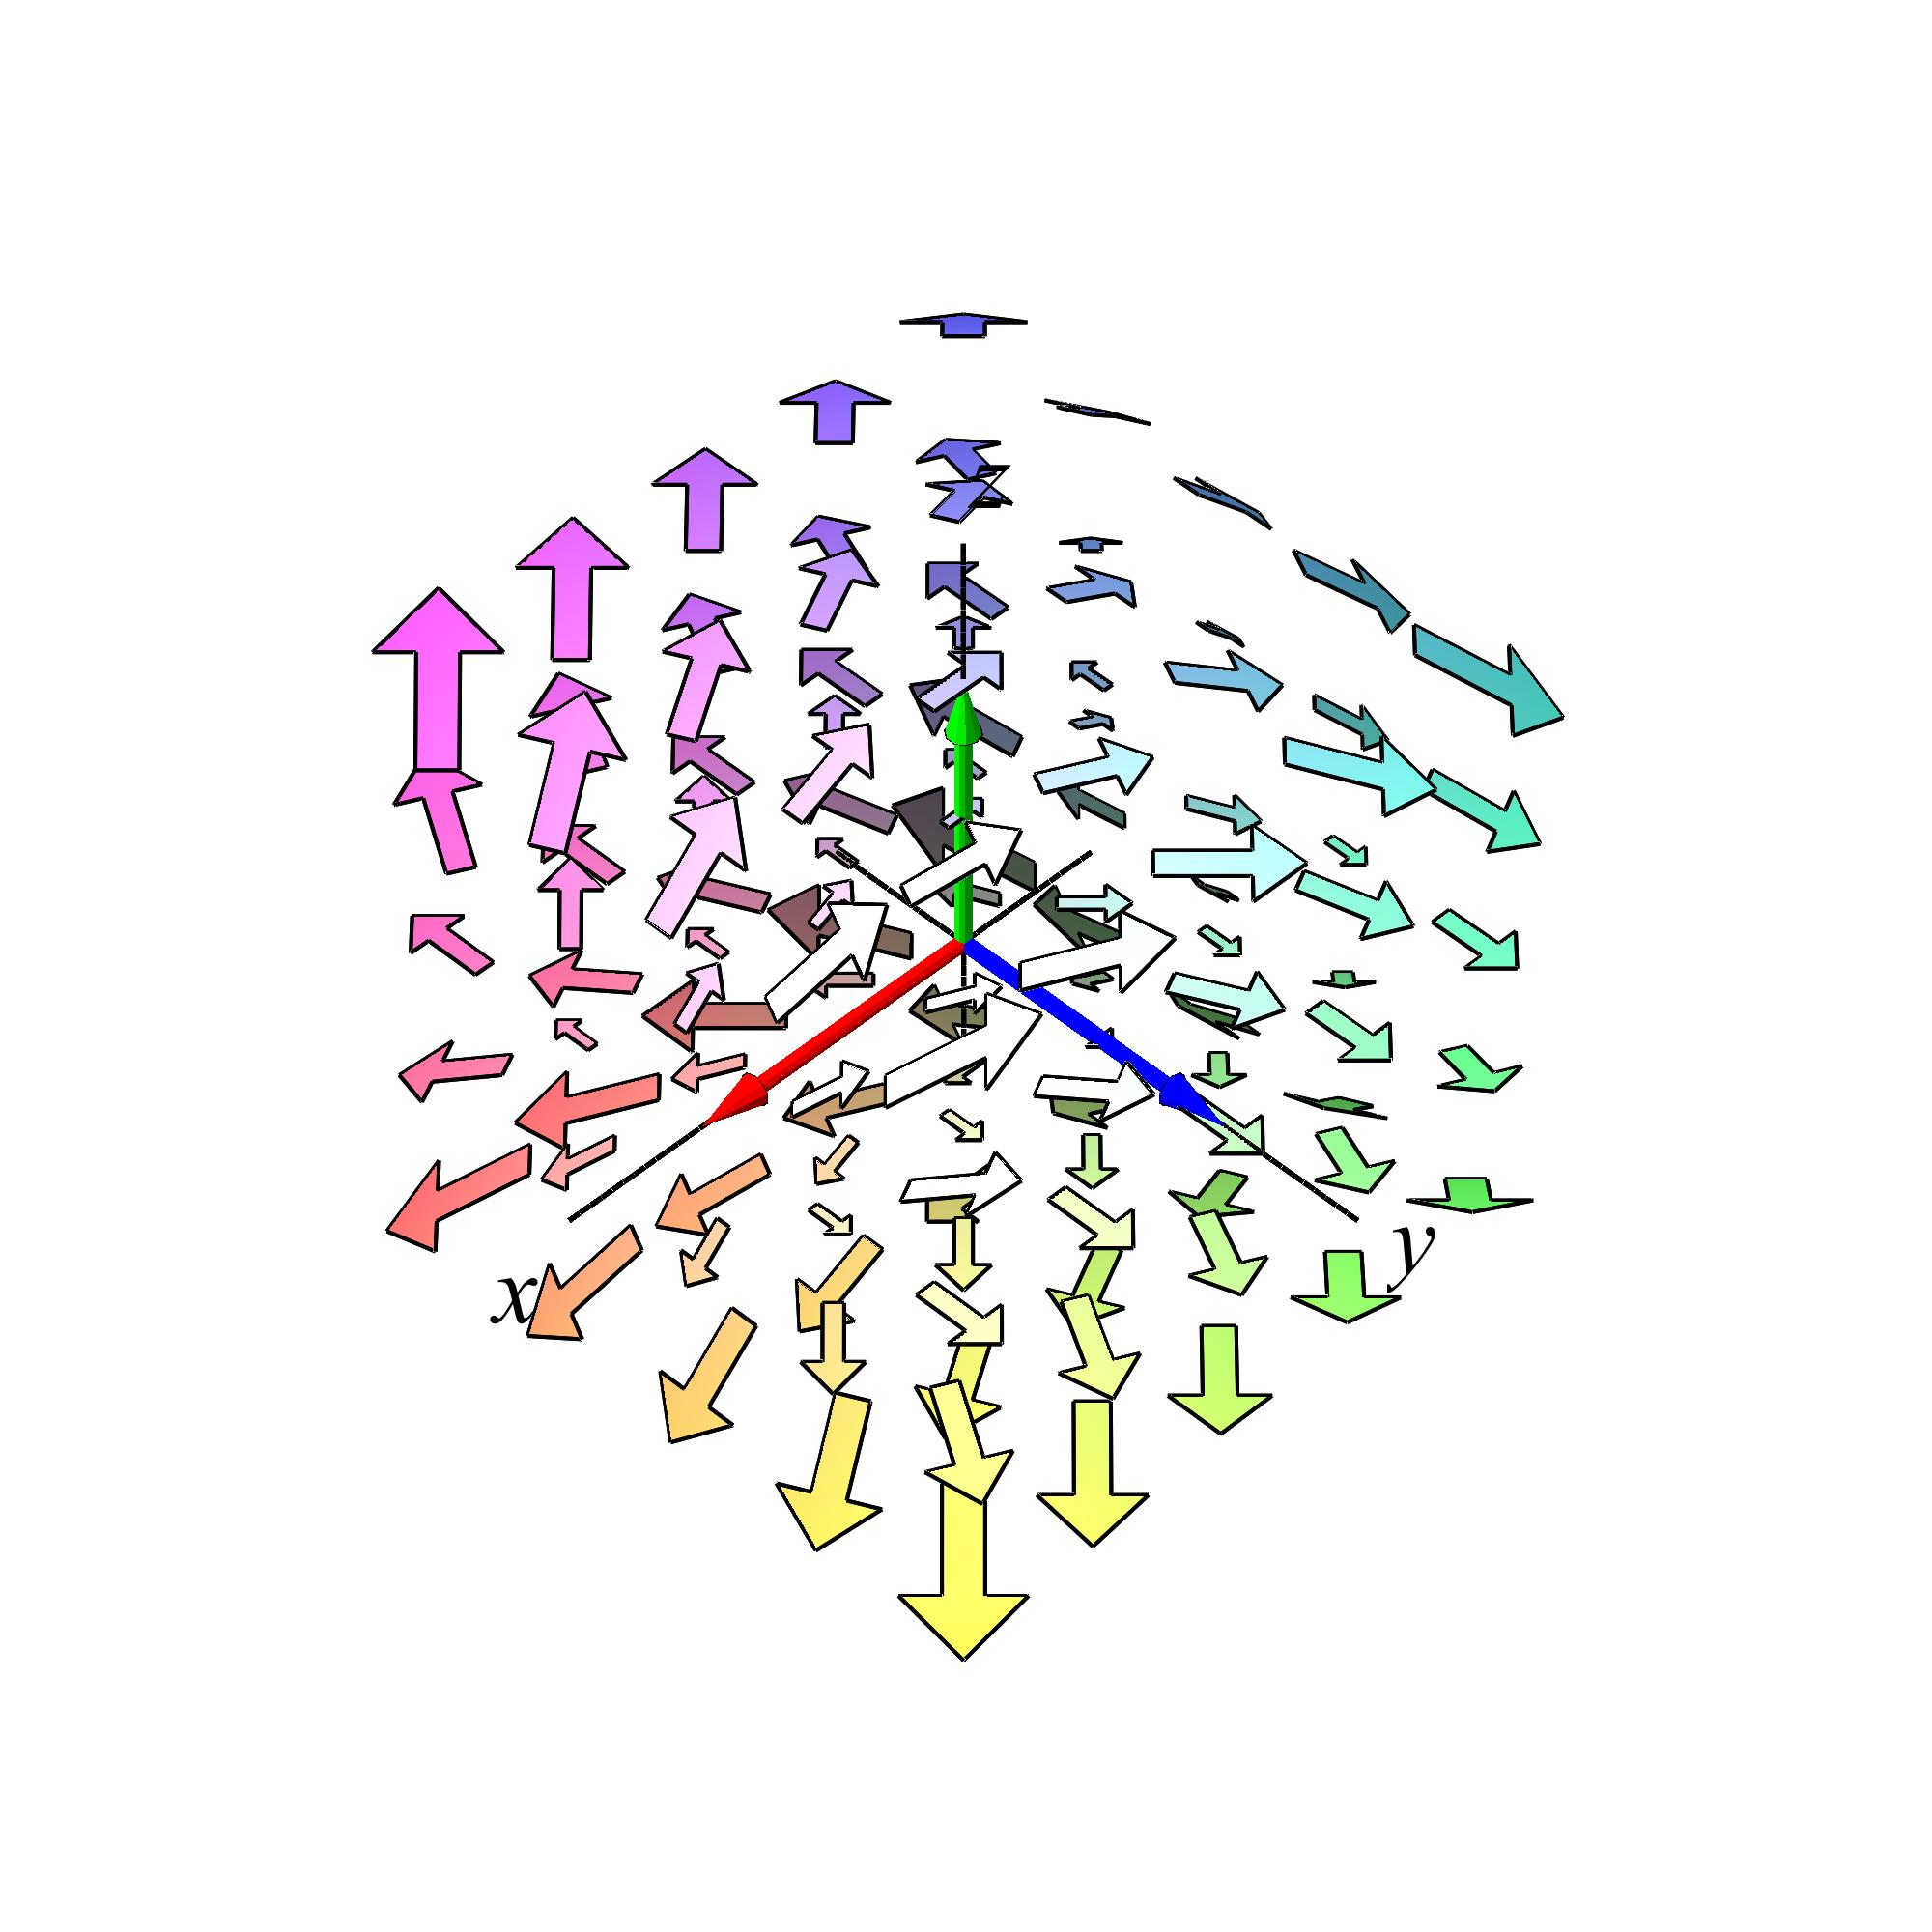
\includegraphics[width=70mm]{FIGS/plotTorusGauss1}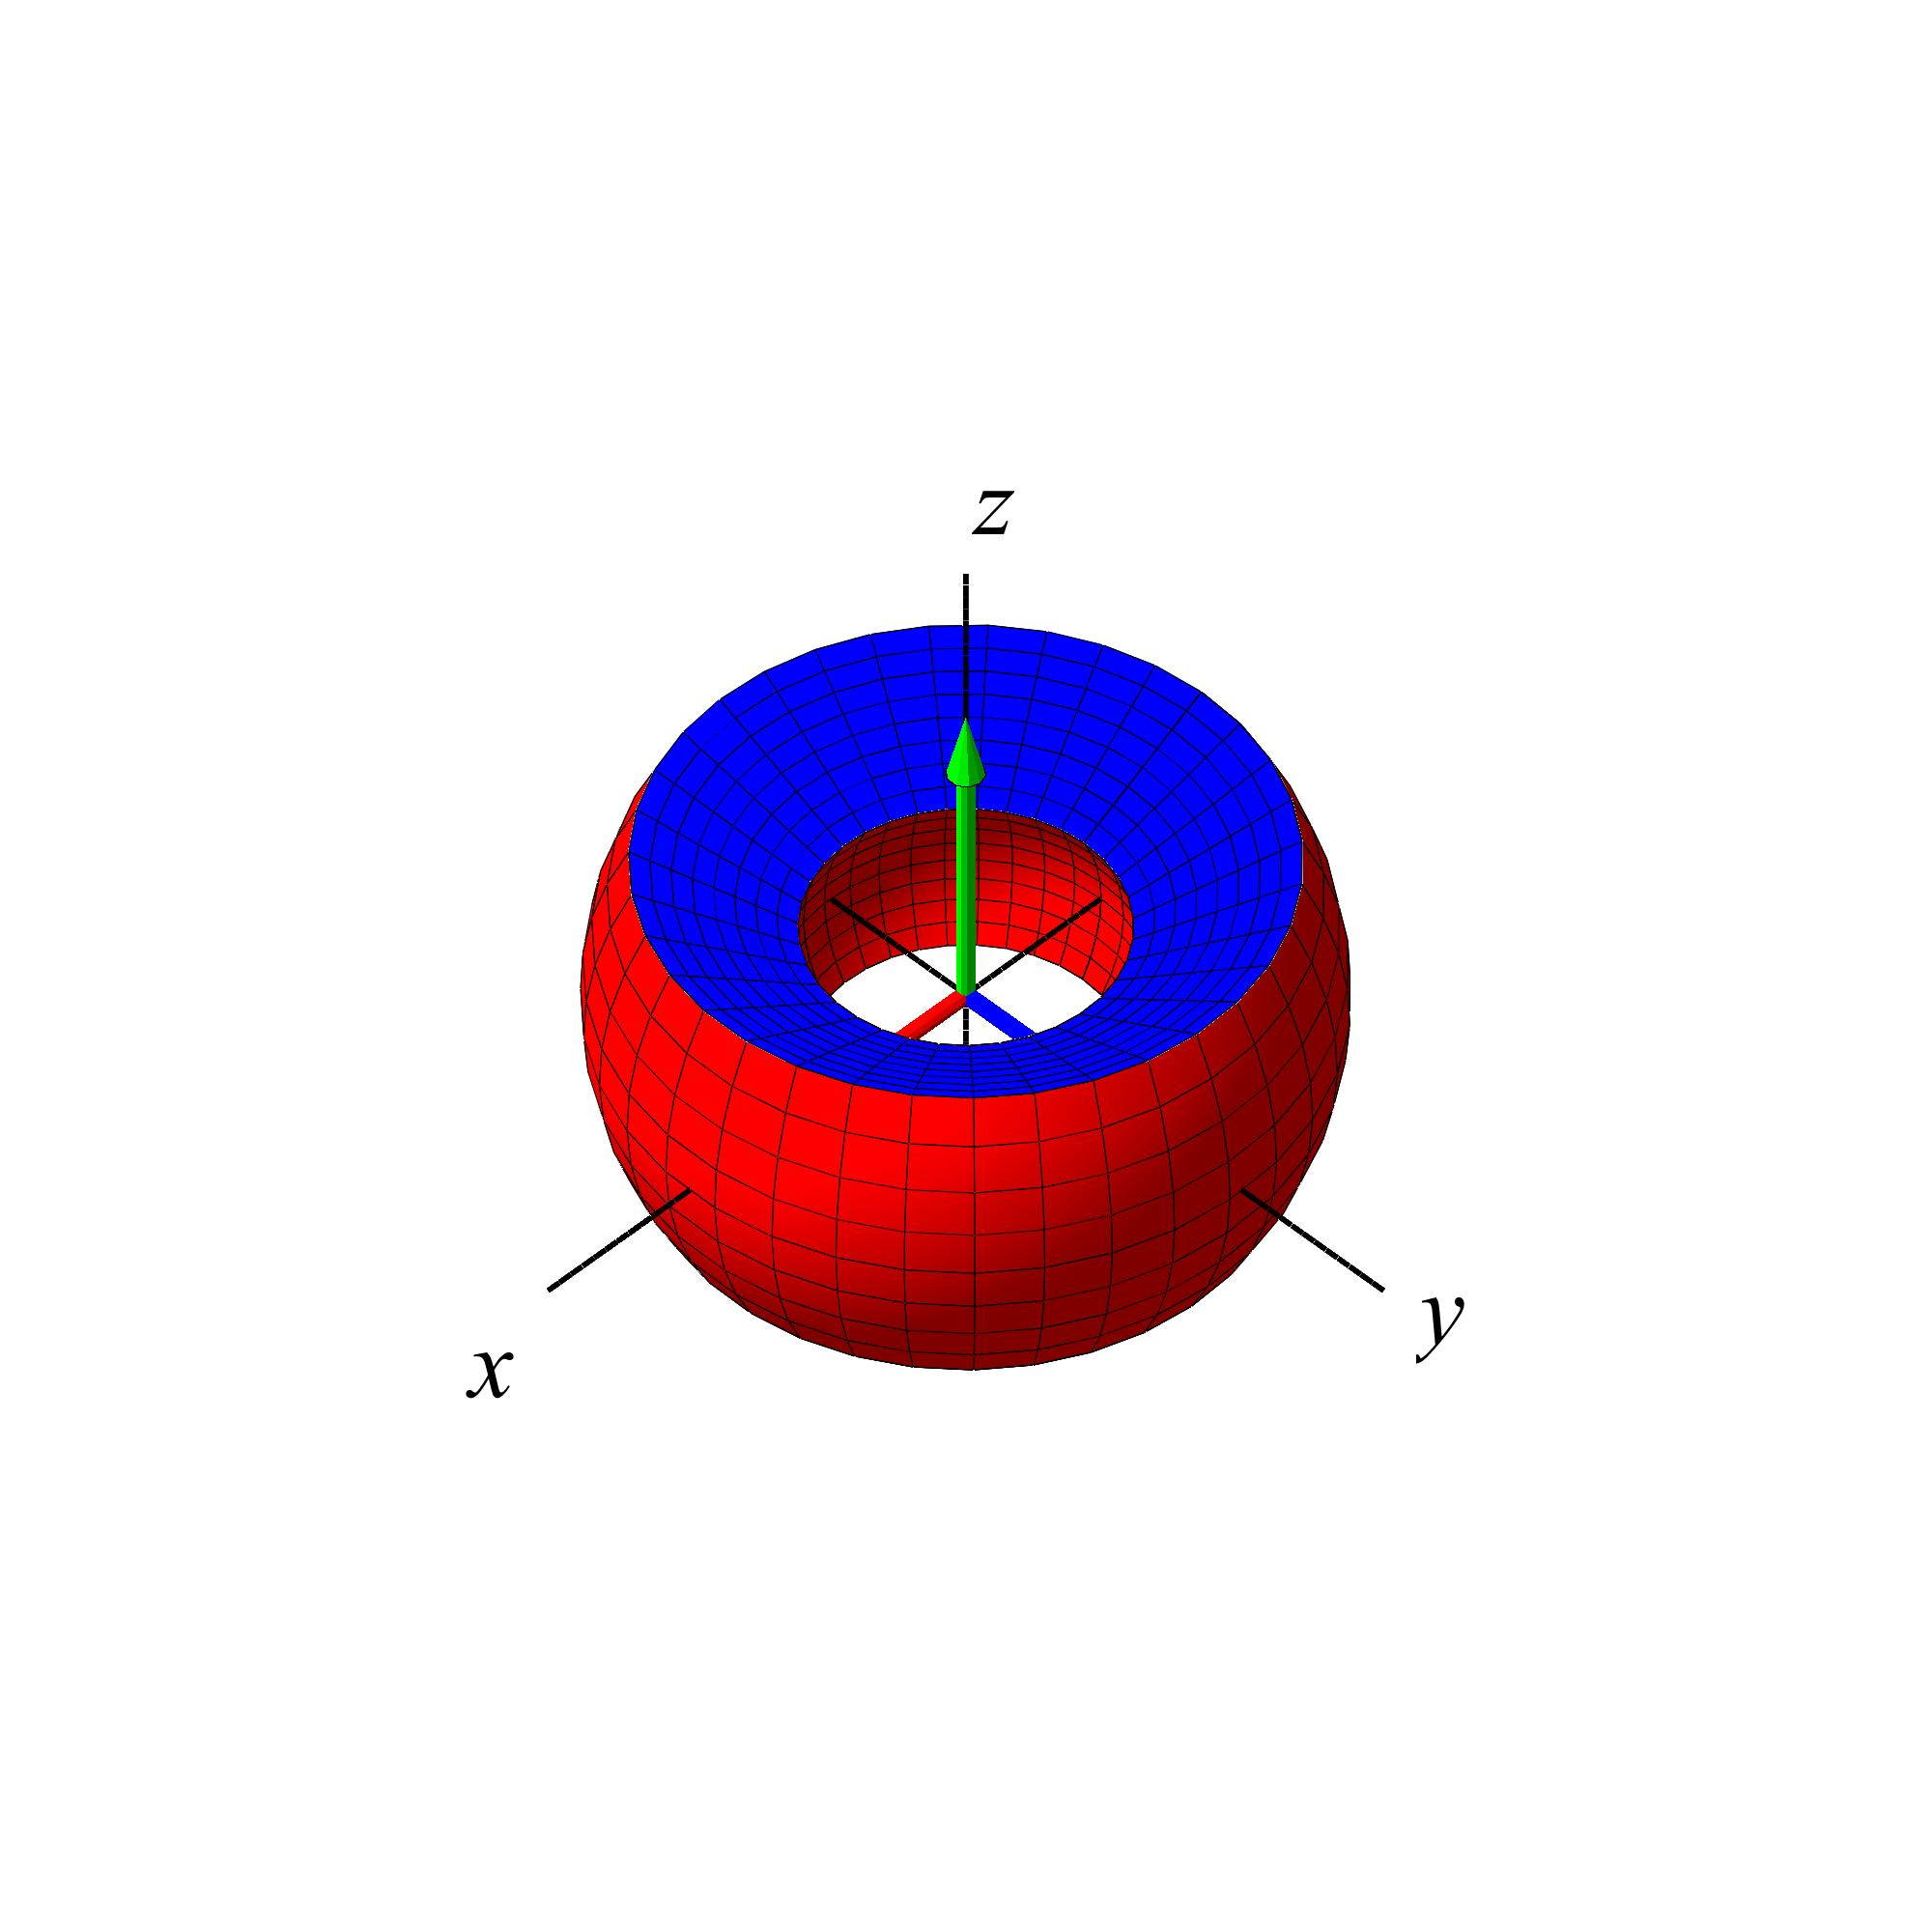
\includegraphics[width=70mm]{FIGS/plotTorusGauss2}}
\begin{center}
\caption{\small{Et vektorfelt omkring og igennem en kantet torus.}} \label{figTorusGauss}
\end{center}
\end{figure}


\section{En konsekvens for rotationsfelter} \label{secKonsekvens}
Vi nævner her en observation, som følger direkte af Gauss' divergenssætning i kombination med følgende  lokale information om rotationsvektorfelter:

\begin{theorem}[Divergensen af et rotationsvektorfelt er 0] \label{thmDivRot}
Lad $\mathbf{V}(x,y,z)$ betegne et glat vektorfelt, som selv er rotationen af et vektorfelt $\mathbf{W}(x,y,z)$ i rummet.
Så er
\begin{equation}
\Div(\mathbf{V})(x,y,z) = 0 \quad.
\end{equation}
Rotationsvektorfelter er altså divergensfrie:
\begin{equation}
\Div(\Rot(\mathbf{W}))(x,y,z) = 0 \quad.
\end{equation}
\end{theorem}
\begin{bevis}
Vi ved pr. antagelse at
\begin{equation}
\mathbf{V}(x,y,z) = (\frac{\partial W_{3}}{\partial y} - \frac{\partial W_{2}}{\partial z}, \, \frac{\partial W_{1}}{\partial z} - \frac{\partial W_{3}}{\partial x}, \, \frac{\partial W_{2}}{\partial x} - \frac{\partial W_{1}}{\partial y}) \quad,
\end{equation}
sådan at
\begin{equation}
\Div(\mathbf{V})(x,y,z) = \left(\frac{\partial^{2} W_{3}}{\partial y \partial x } - \frac{\partial^{2} W_{2}}{\partial z \partial x }\right) + \left(\frac{\partial^{2} W_{1}}{\partial z \partial y} -\frac{\partial^{2} W_{3}}{\partial x \partial y}\right) + \left(\frac{\partial^{2} W_{2} }{\partial x \partial z } - \frac{\partial^{2} W_{1}}{\partial y \partial z}\right) = 0 \, \, ,
\end{equation}
hvor vi har benyttet, at differentiationsordenen kan ombyttes, e.g.:
\begin{equation}
\frac{\partial^{2} W_{3}}{\partial y \partial x } = \frac{\partial^{2} W_{3}}{\partial x \partial y } \quad .
\end{equation}
\end{bevis}

Hvis vi bruger sætning  \ref{thmDivRot} i kombination med Gauss' sætning får vi

\begin{corollary}[Totale flux af et rotationsvektorfelt er 0] \label{corTotFlux0}
Lad $\mathbf{W}(x,y,z)$ betegne et glat vektorfelt i rummet og lad $\Omega$ være et område i rummet med stykkevis glat overflade $\partial \Omega$ med udadrettet enhedsnormalvektorfelt $\mathbf{n}_{\partial \Omega}$. \\

Så er den \emph{totale flux} af $\Rot(\mathbf{W})(x,y,z)$ ud gennem overfladen $\partial \Omega$ af $\Omega$ lig med $0$:
\begin{equation}
\Flux(\Rot(\mathbf{W}), \partial \Omega) = \int_{\partial \Omega}\Rot(\mathbf{W})\bm{\cdot} \mathbf{n}_{\partial \Omega} \, d\mu \, = \, 0 \quad .
\end{equation}
Hvis det rumlige område flyder med flowkurverne for $\Rot(\mathbf{W}(x,y,z)$ så er rumfanget konstant under hele flowdeformationen:
\begin{equation}
\frac{d}{dt}\Vol_{\pm}(t) = 0 \quad \textrm{for \emph{alle}} \quad  t  \quad.
\end{equation}
\end{corollary}


\begin{figure}[ht]
\centerline{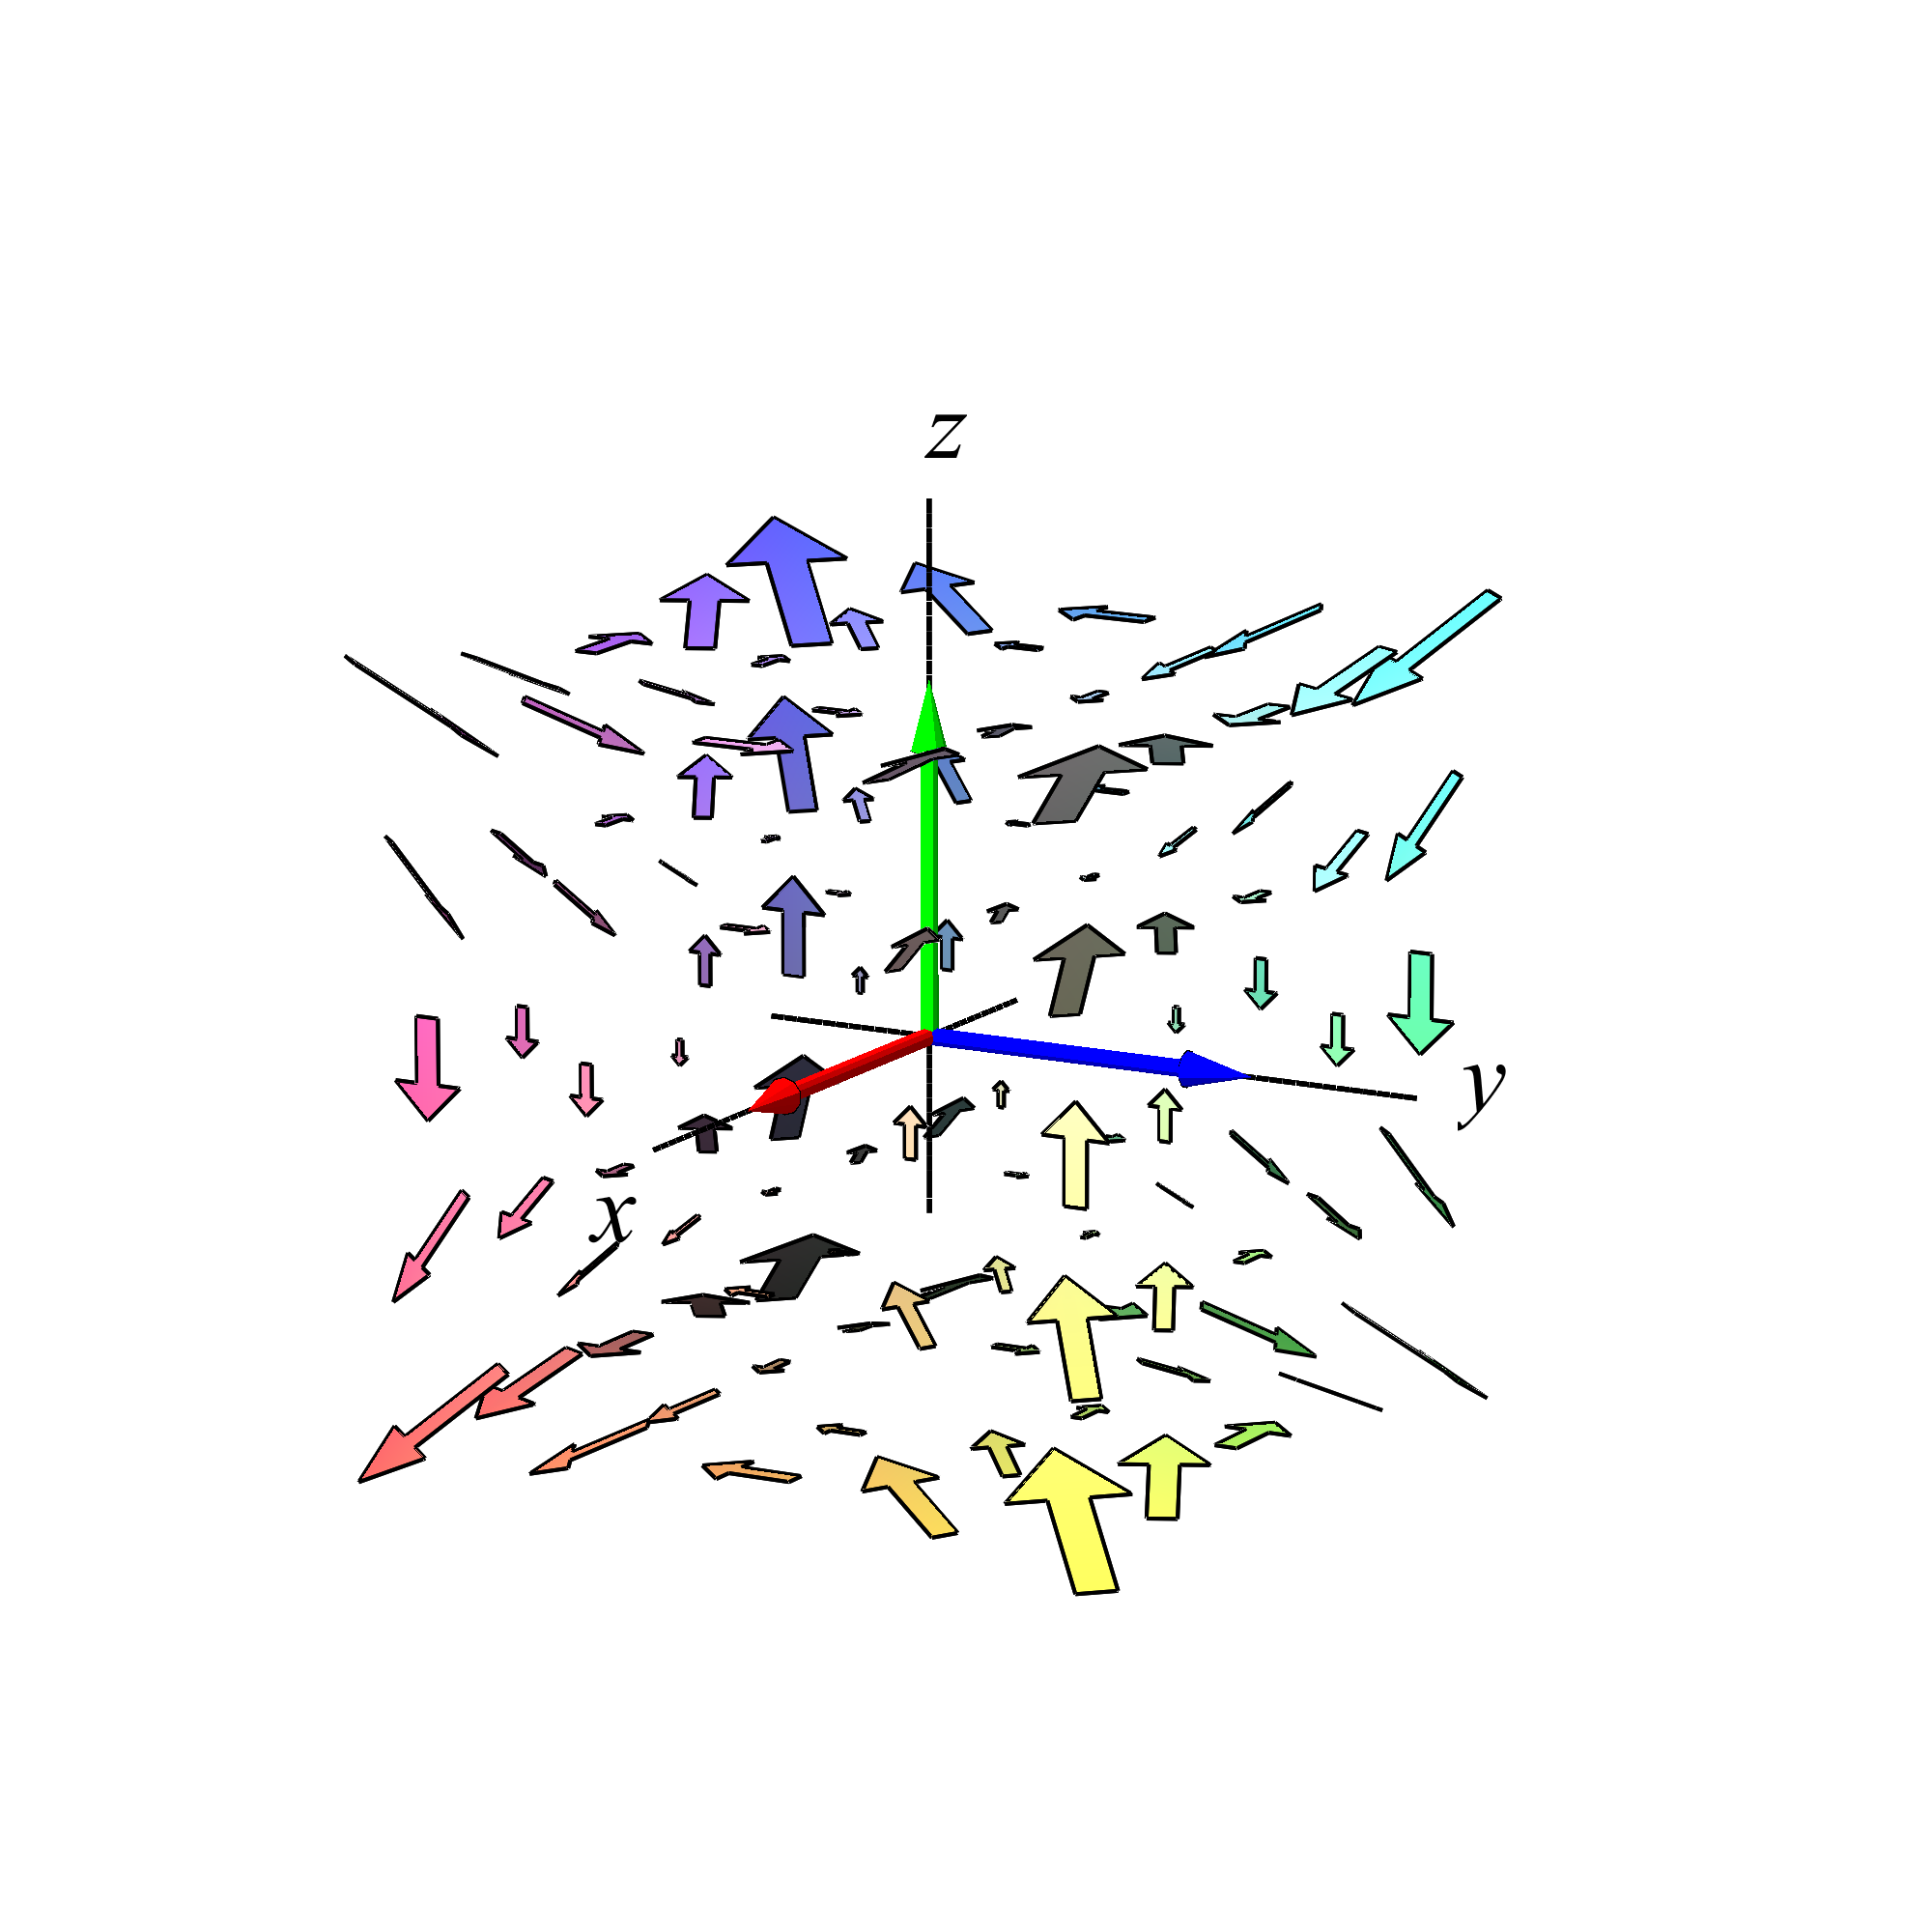
\includegraphics[width=70mm]{FIGS/plotKugleFluxRot2}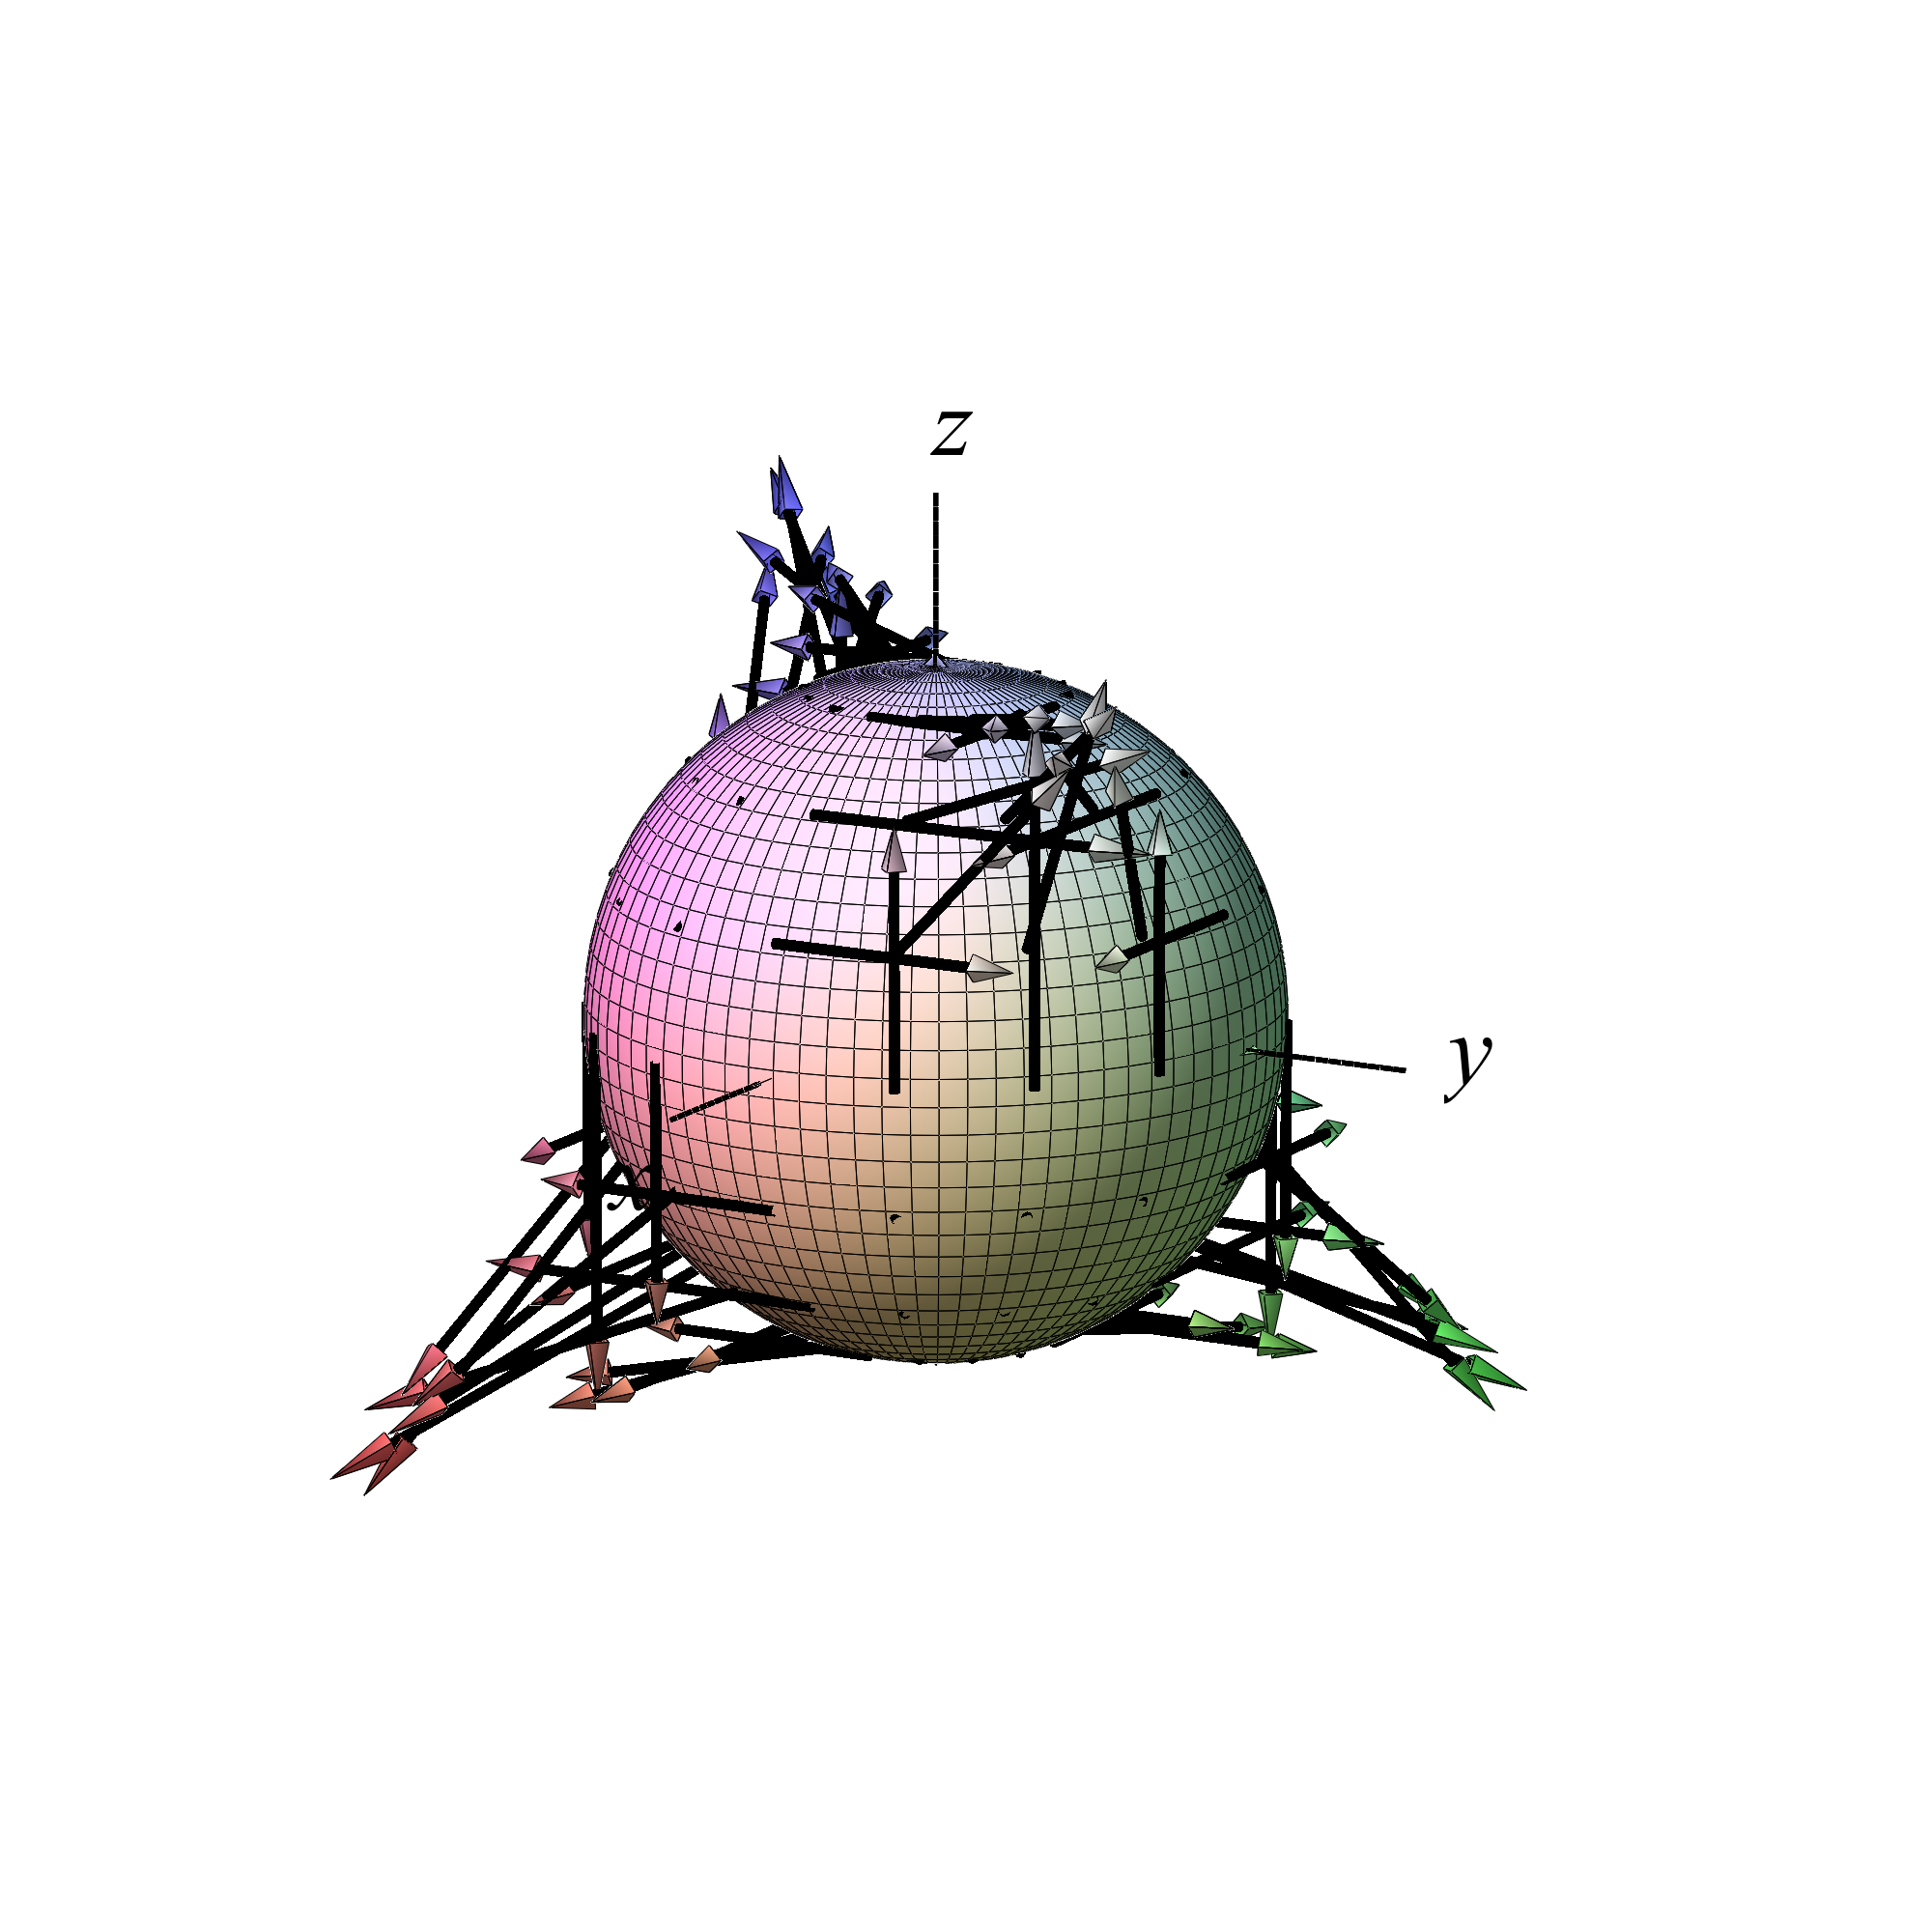
\includegraphics[width=70mm]{FIGS/plotKugleFluxRot3}}
\begin{center}
\caption{\small{Et rotationsvektorfelt $\mathbf{V}(x,y,z) = \Rot(\mathbf{W})(x,y,z)$ omkring og igennem en kugle. Den totale flux ud igennem kuglefladen er $0$, men den lokale flux ud igennem passende valgte fladestykker af kuglefladen er tydeligvis ikke $0$.}} \label{figKugleFluxRot}
\end{center}
\end{figure}


\begin{example}[Et rotationsvektorfelt igennem en kugle] \label{exampRotFeltFlux}
Vi lader $\mathbf{W}(x,y,z) = (z^{2}\cdot x, x^{2}\cdot y, y^{2}\cdot z)$. \\

 Så er
\begin{equation}
\Rot(\mathbf{W})(x,y,z) = (2\cdot y \cdot z, \, 2\cdot z \cdot x, \, 2\cdot x \cdot y ) \quad,
\end{equation}
samt tydeligvis
\begin{equation}
\Div(\Rot(\mathbf{W}))(x,y,z) = 0 \quad.
\end{equation}
Lad nu $F_{\mathbf{r}}$ betegne kuglefladen med radius $1$ placeret med centrum i $(0,0,0)$:
\begin{equation}
F_{\mathbf{r}} \quad : \quad \mathbf{r}(u,v) = (x(u,v), y(u,v), z(u,v)) = (\sin(u)\cdot \cos(v), \sin(u)\cdot \sin(v), \cos(u)) \quad ,
\end{equation}
hvor $u \in [0, \pi]$ og $v \in [-\pi, \pi]$. Som bekendt er Jacobifunktionen for denne parametrisering af kuglefladen givet ved:
\begin{equation}
\Jac_{\mathbf{r}}(u,v) = \sin(u) \quad ,
\end{equation}
og enhedsnormalvektoren til kuglefladen er i dette specielle tilfælde:
\begin{equation}
\mathbf{n}_{F}(u,v) = (x(u,v), y(u,v), z(u,v)) \quad ,
\end{equation}
sådan at
\begin{equation}
\begin{aligned}
\Rot(\mathbf{W})(x,y,z)\bm{\cdot} \mathbf{n}_{F}(u,v) &= 2\cdot(y\cdot z, \, y\cdot z, \, y\cdot z ) \bm{\cdot} (x, y, z) \\
&= 6\cdot x(u,v) \cdot y(u,v) \cdot z(u,v) \\
&= 6 \cdot \sin^{2}(u) \cdot \cos(v) \cdot \sin(v) \cdot \cos(u) \quad .
\end{aligned}
\end{equation}
Det totale flux-integral af $\Rot(\mathbf{W})(x,y,z)$ ud igennem kuglefladen er derfor:
\begin{equation} \label{eqIntegrat}
\begin{aligned}
\Flux(\Rot(\mathbf{W}), F_{\mathbf{r}}) &= \int_{F_{\mathbf{r}}}\Rot(\mathbf{W})\bm{\cdot} \mathbf{n}_{F} \, d\mu \\
&= \int_{-\pi}^{\pi}\int_{0}^{\pi} \left( 6 \cdot \sin^{2}(u) \cdot \cos(v) \cdot \sin(v) \cdot \cos(u)\right) \cdot \Jac_{\mathbf{r}}(u,v) \,\, du \, dv \\
&= \int_{-\pi}^{\pi}\int_{0}^{\pi} \left( 6 \cdot \sin^{2}(u) \cdot \cos(v) \cdot \sin(v) \cdot \cos(u)\right) \cdot \sin(u) \,\, du \, dv \\
&= \int_{-\pi}^{\pi}\int_{0}^{\pi} 6 \cdot \sin^{3}(u) \cdot \cos(v) \cdot \sin(v) \cdot \cos(u) \,\, du \, dv \\
\end{aligned}
\end{equation}
og da en stamfunktion til $\sin^{3}(u)\cdot \cos(u)$ er $\frac{1}{4}\cdot \sin^{4}(u)$ som er $0$ både for $u=0$ og for $u=\pi$,
så er
\begin{equation}
\Flux(\Rot(\mathbf{W}), F_{\mathbf{r}}) = 0
\end{equation}
i overensstemmelse med følgesætning \ref{corTotFlux0}.
\end{example}

\begin{think}
Læg mærke til, at hvis integrationsintervallerne for $u$ og $v$  i ligning (\ref{eqIntegrat}) i eksempel \ref{exampRotFeltFlux}  havde været
mindre, dvs. hvis vi havde betragtet fluxen af rotationsvektorfeltet ud igennem \emph{en del af} kugleoverfladen, så ville resultatet ikke nødvendigvis blive $0$, hvilket også fremgår tydeligt af figur \ref{figKugleFluxRot}. \\

Fluxen af $\Rot(\mathbf{W}(x,y,z)$ igennem et fladestykke kan alternativ beregnes som cirkulationen  af $\mathbf{W}(x,y,z)$ langs med fladestykkets rand -- det er indholdet af Stokes' sætning, som er emnet for eNote 27.
\end{think}



\begin{figure}[ht]
\centerline{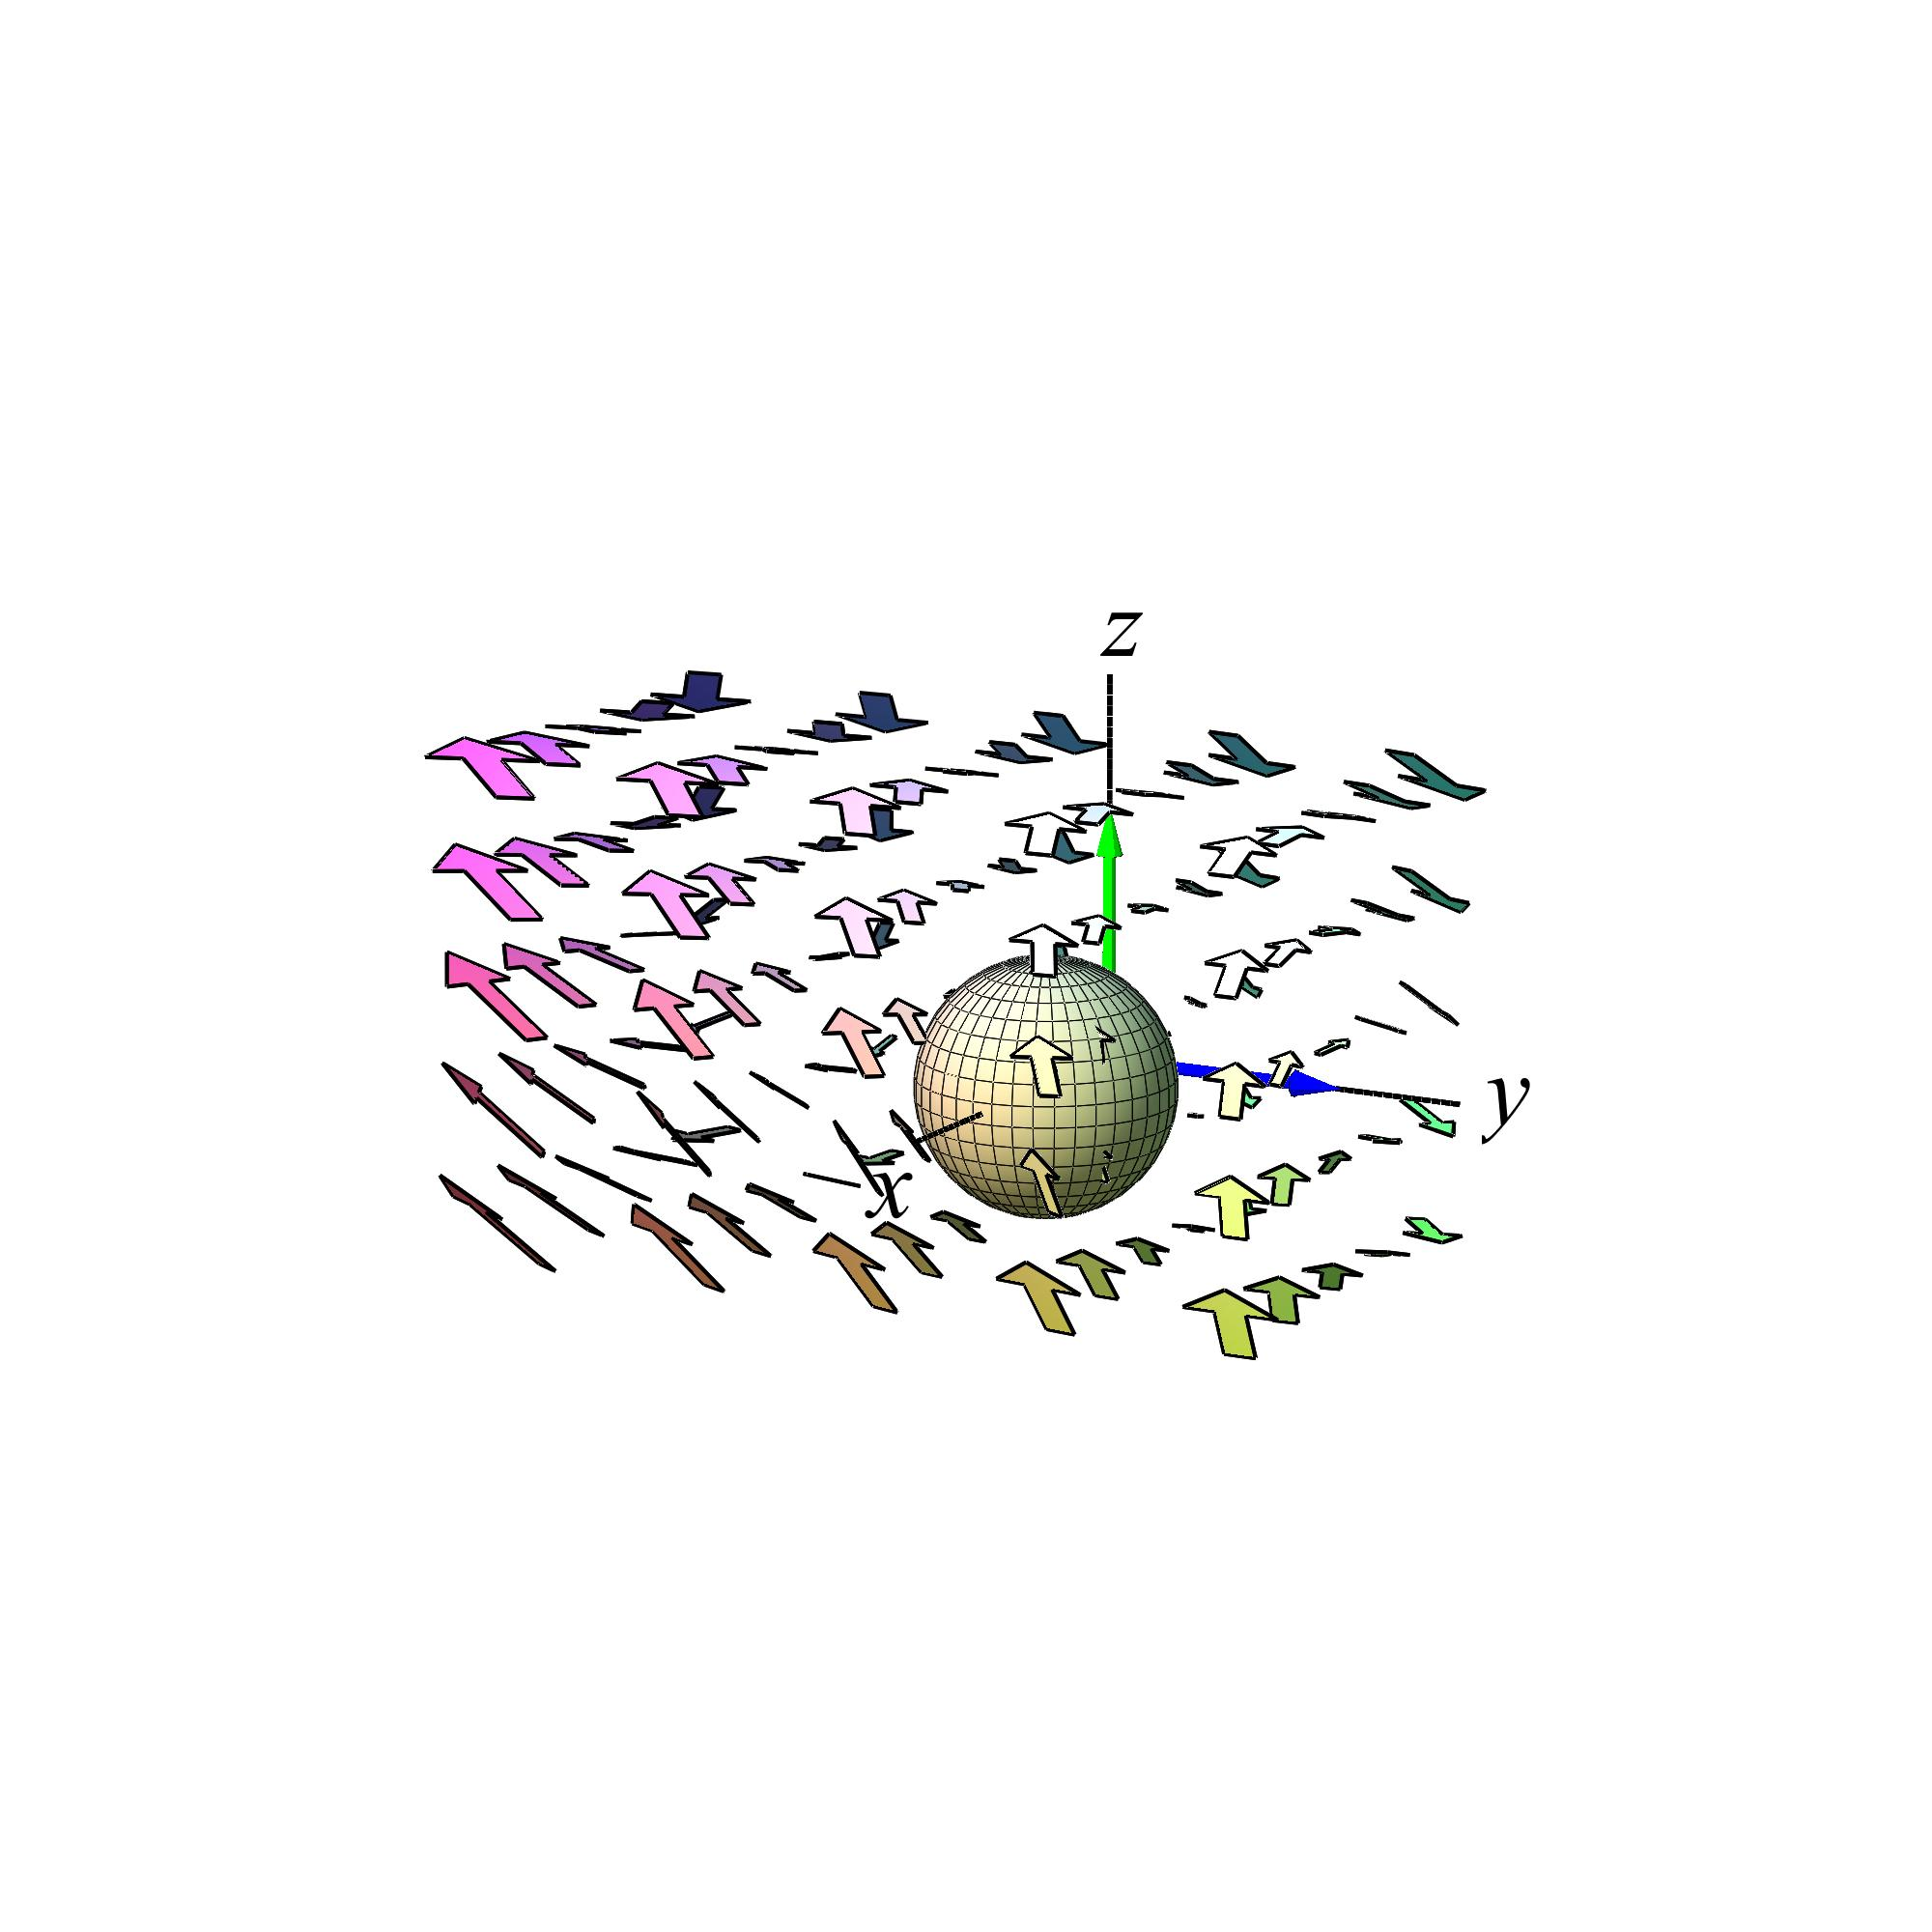
\includegraphics[width=70mm]{FIGS/plotSphFlowRot1}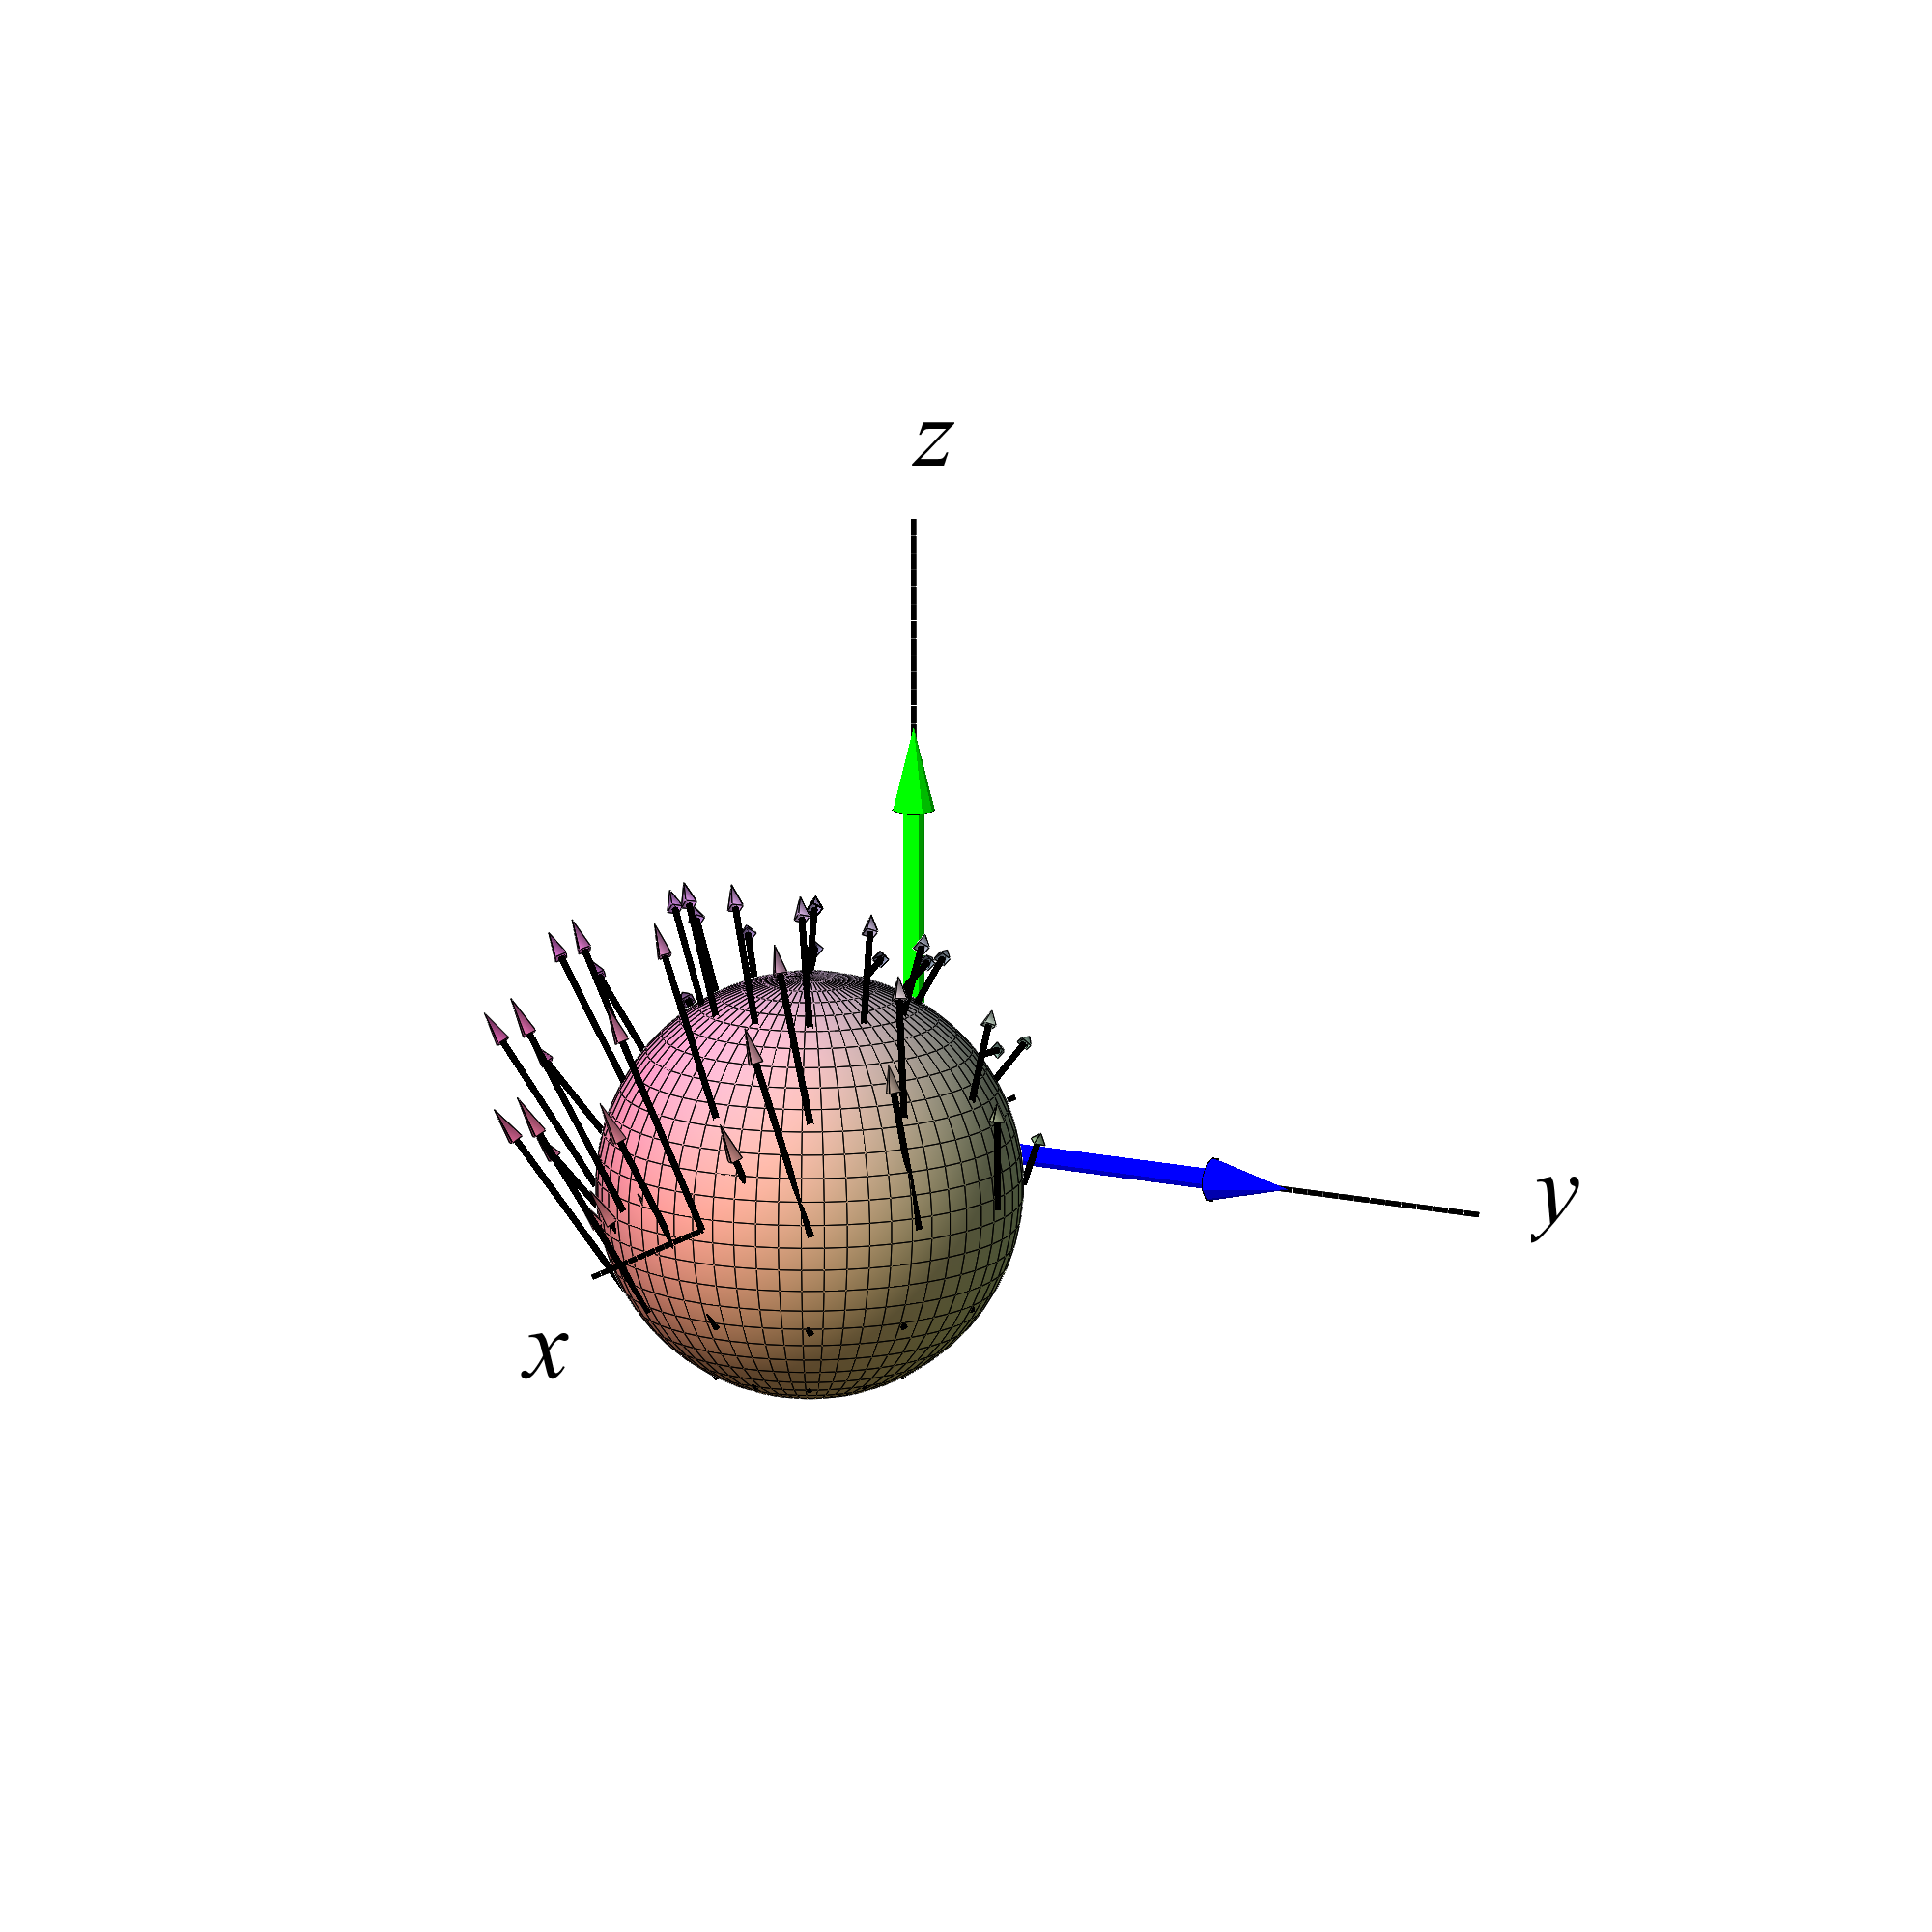
\includegraphics[width=70mm]{FIGS/plotSphFlowRot2} 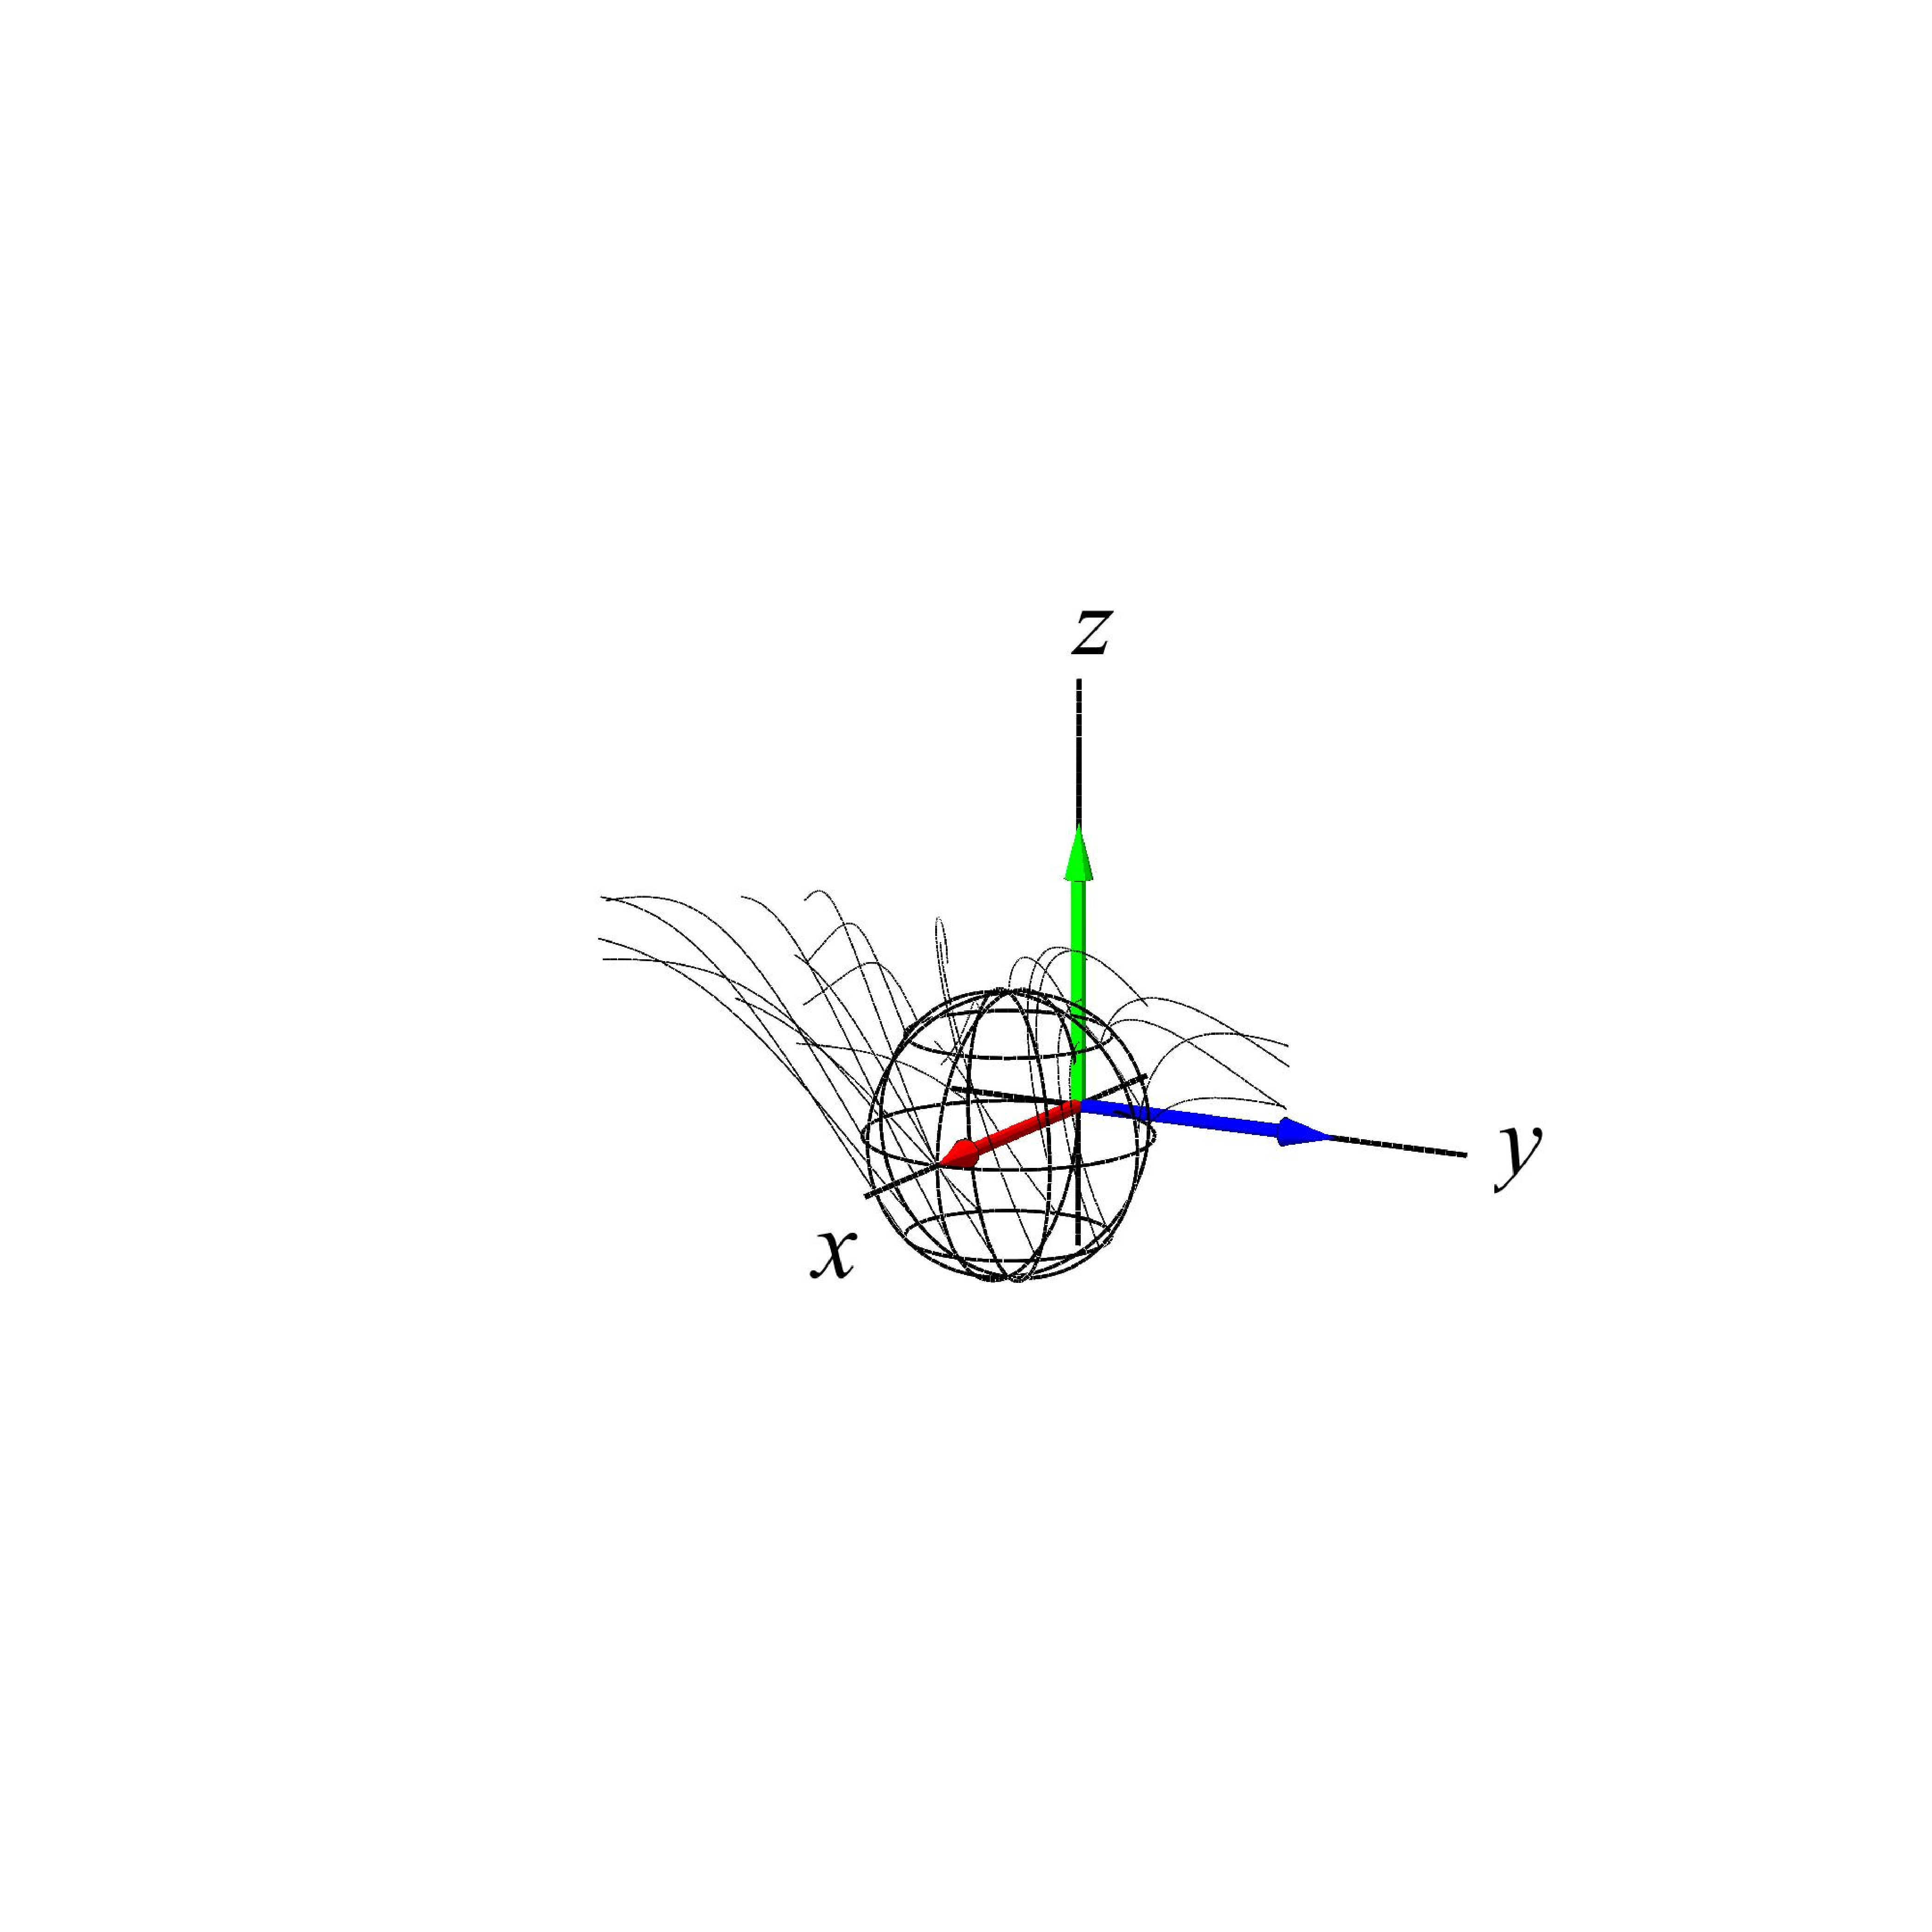
\includegraphics[width=70mm]{FIGS/plotSphFlowRot3}}
\begin{center}
\caption{\small{Et divergensfrit vektorfelt $\mathbf{V}(x,y,z) = (-z, (y-x)/2, x-(z/2))$ omkring og igennem en kugle.}} \label{figSphFlowRotA}
\end{center}
\end{figure}


\begin{figure}[ht]
\centerline{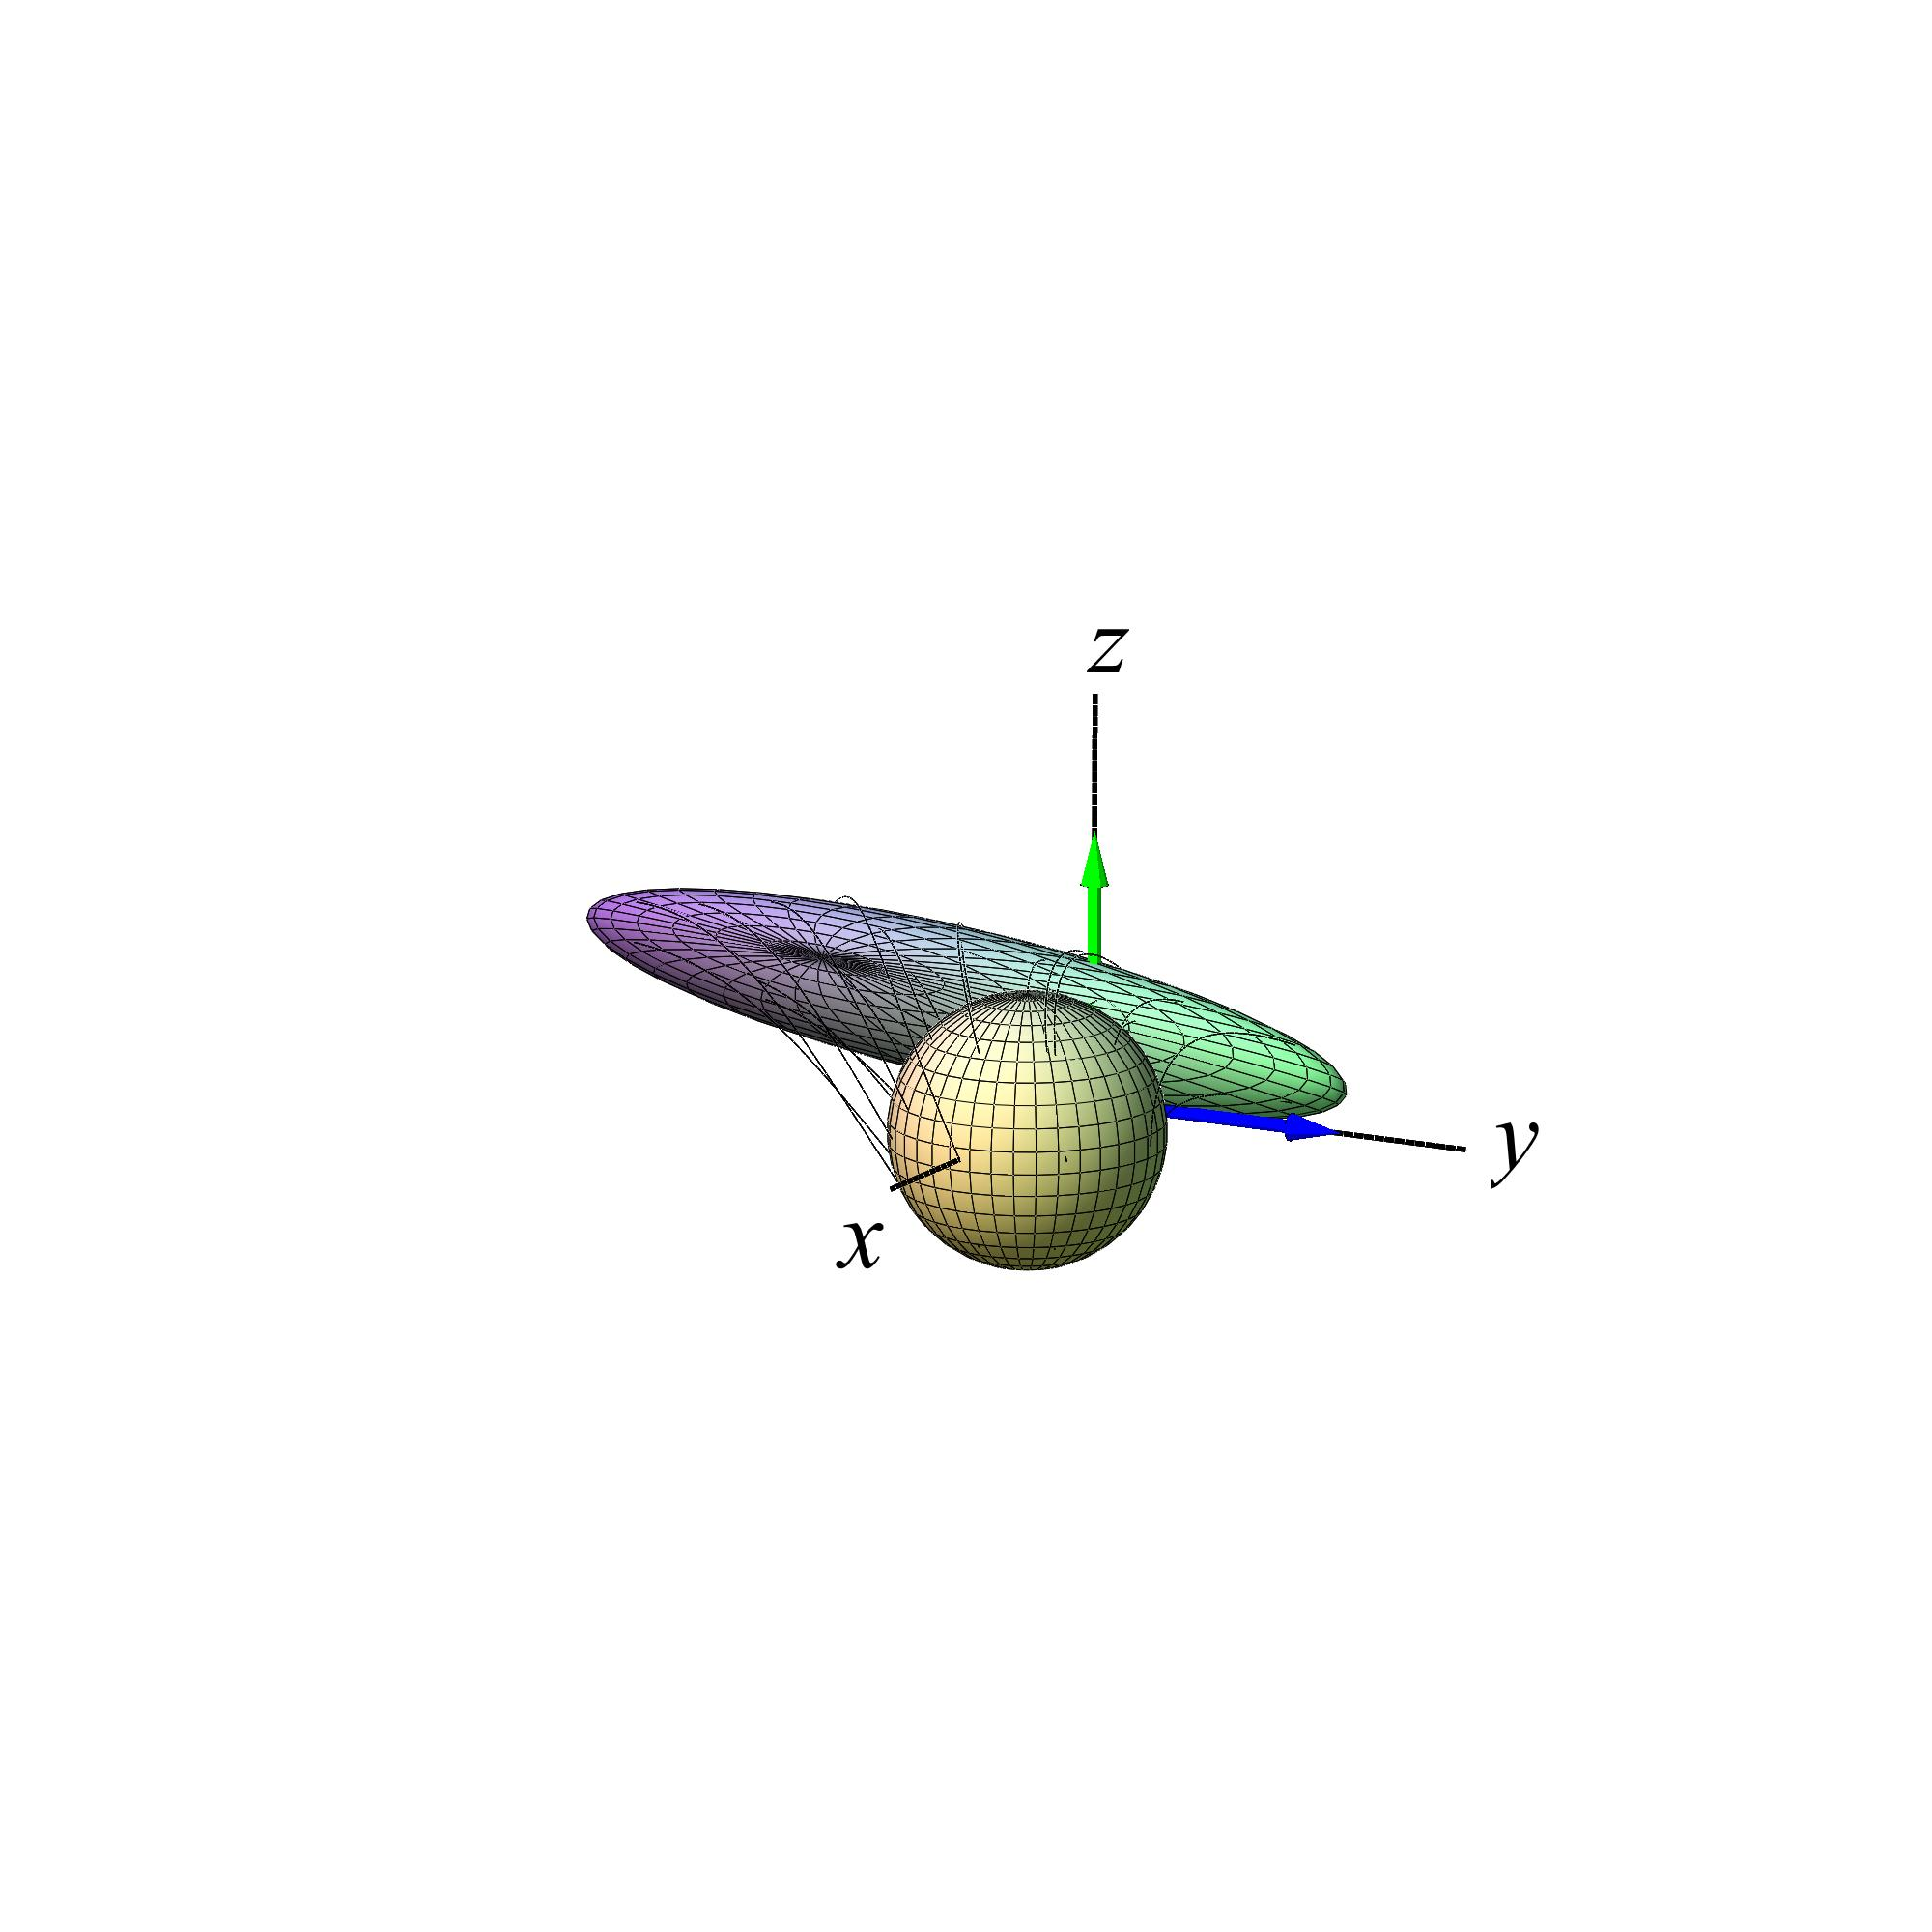
\includegraphics[width=85mm]{FIGS/plotSphFlowRot4}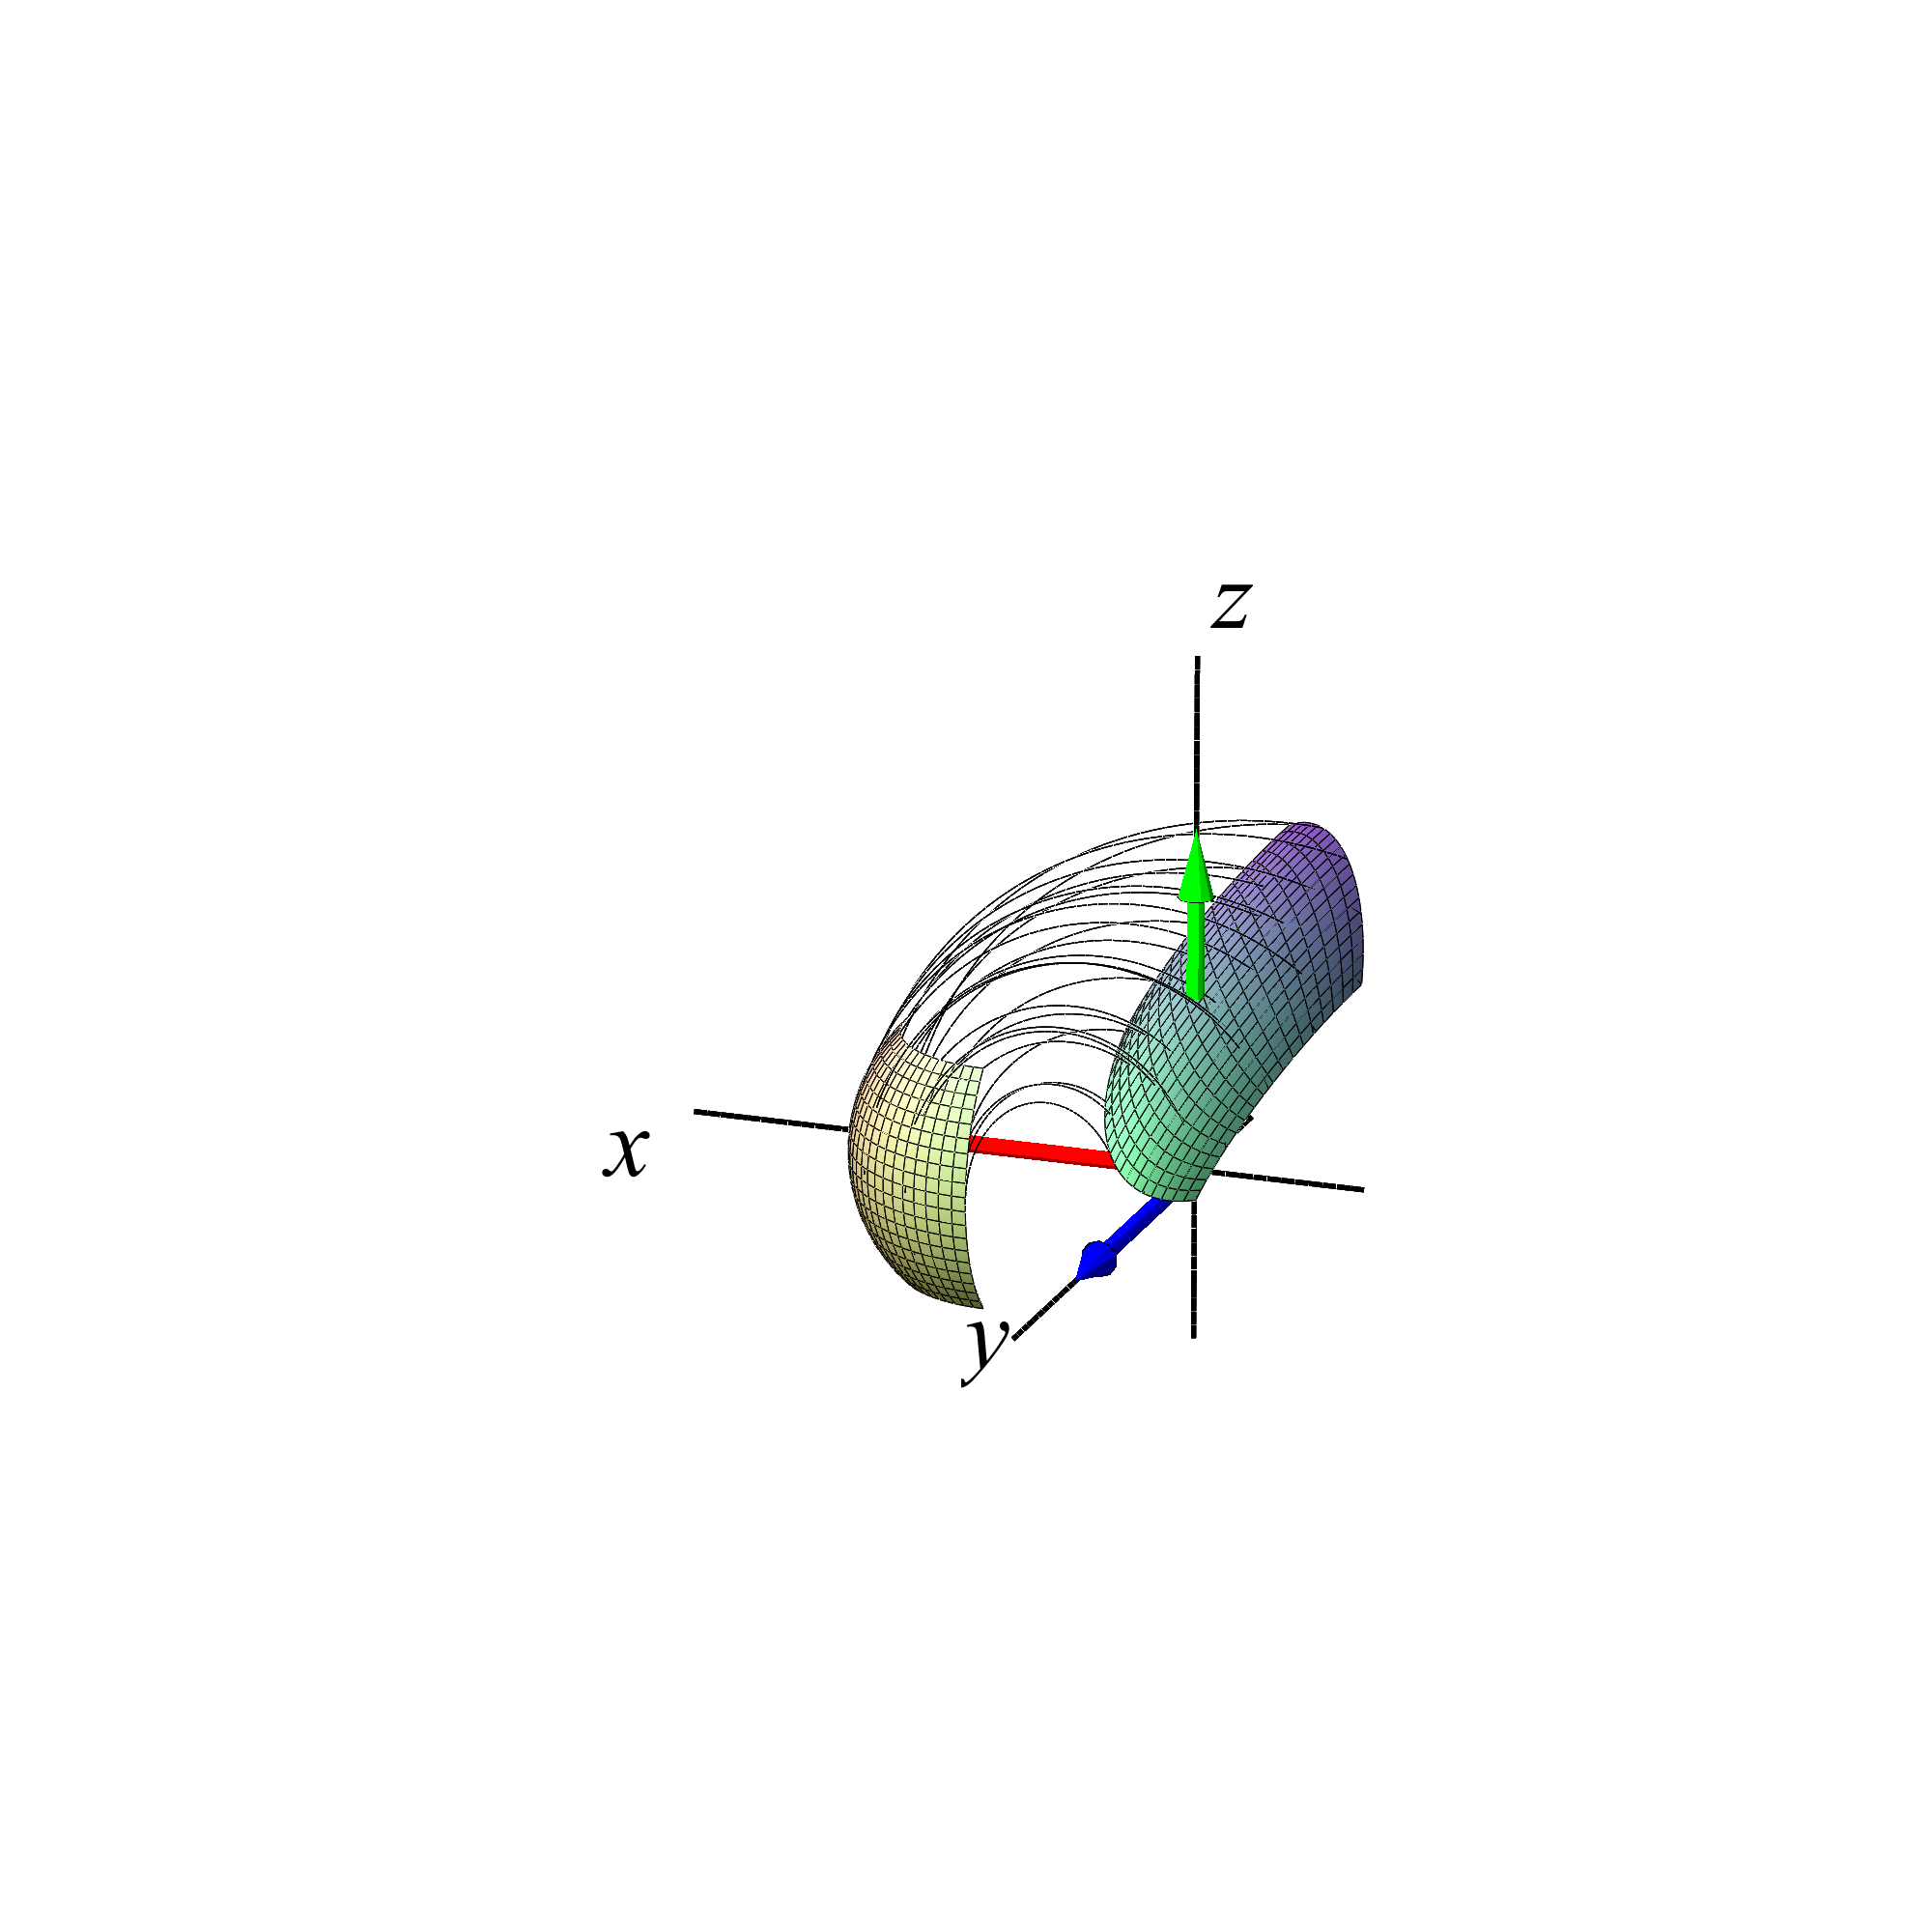
\includegraphics[width=85mm]{FIGS/plotSphPartFlowRot}}
\begin{center}
\caption{\small{Det divergensfrie vektorfelt $\mathbf{V}(x,y,z) = (-z, (y-x)/2, x-(z/2))$ deformerer en massiv kugle til en massiv ellipsoide ved at alle kuglens punkter flyder med  flowkurverne for vektorfeltet. Rumfanget er bevaret. Til højre er vist, hvordan et udsnit af kugleoverfladen flyder og danner en del af ellipsoide-overfladen.}} \label{figSphFlowRotB}
\end{center}
\end{figure}

\begin{example}[Divergensfrit førstegrads-vektorfelt]\label{exampFirstDiv0}
Første-grads vektorfeltet
\begin{equation}
\mathbf{V}(x,y,z) =  (-z, (y-x)/2, x-(z/2))
\end{equation}
har divergensen $\Div(\mathbf{V})(x,y,z) = 0$. Den totale flux af vektorfeltet ud igennem overfladen af ethvert rumligt område er derfor $0$ og rumfanget af det rumlige område er bevaret ved flow med vektorfeltets flowkurver. \\

For første-gradsvektorfelter gælder, at enhver massiv kugle deformeres igennem massive \emph{ellipsoider} ved at flyde med vektorfeltet, se figur \ref{figSphFlowRotA}, figur \ref{figSphFlowRotB} og opgave \ref{exercDiffSys}.
\end{example}

\begin{exercise}[(Advanced)]\label{exercDiffSys}
Lad $\mathbf{V}(x,y,z)$ betegne et vilkårligt førstegrads-vektorfelt (se \tref{NUID40-tn24}{eNote}) og lad $F_{0}$ betegne en vilkårlig niveauflade for et givet andengradspolynomium $f_{0}(x,y,z)$ i $x$, $y$, og $z$ (se \tref{NUID35-tn20}{eNote}). Vi lader så  $F_{0}$ flyde tiden $t$ med flowkurverne for $\mathbf{V}(x,y,z)$ og får derved en flade $F_{t}$. Vis, at $F_{t}$ også er en niveauflade for et andengradspolynomium $f_{t}(x,y,z)$ i $x$, $y$, og $z$. Vink: Se \tref{NUID13-tn12}{eNote}.
\end{exercise}



%%%%%%%%%%%%%%%%%%%%%%%%%%%%%%%%%%%%%%%%%%%%%%%%%%%%%%%%%%%%%%%%%%%%%%%%%
%%%%%%%%%%%%%%%%%%%%%%%%%%%%%%%%%%%%%%%%%%%%%%%%%%%%%%%%%%%%%%%%%%%%%%%%%
%%%%%%%%%%%%%%%%%%%%%%%%%%%%%%%%%%%%%%%%%%%%%%%%%%%%%%%%%%%%%%%%%%%%%%%%%



%%%%%%%%%%%%%%%%%%%%%%%%%%%%%%%%%%%%%%%%%%%%%%%%%%%%%%%%%%%%%
%%%%%%%%%%%%%%%%%%%%%%%%%%%%%%%%%%%%%%%%%%%%%%%%%%%%%%%%%%%%%
%%%%%%%%%%%%%%%%%%%%%%%%%%%%%%%%%%%%%%%%%%%%%%%%%%%%%%%%%%%%%

\begin{summary}
Vi har indført det fundamentale begreb \emph{flux af et vektorfelt igennem en flade} og relateret fluxen dels til den lokale volumen-ekspansions-rate ved selve fladen når denne flyder med flowkurverne for vektorfeltet, og dels til divergensen af vektorfeltet inde i et rumligt område der er afgrænset af en given overflade.
\begin{itemize}
\item For en glat parametriseret flade $F_{\mathbf{r}}$ og et glat vektorfelt $\mathbf{V}(x,y,z)$ er fluxen af vektorfeltet igennem fladen:
\begin{equation}
\begin{aligned}
\Flux({\bf V}, F_{\bf r})\,&= \, \int_{c}^{d}\int_{a}^{b}{\bf V}({\bf r}(u,v)) \bm{\cdot} ({\bf
r}'_{u}(u,v)\times{\bf r}'_{v}(u,v))\,du \, dv  \\
&= \, \int_{c}^{d}\int_{a}^{b}{\bf V}({\bf r}(u,v)) \bm{\cdot} \mathbf{N}_{F}(u,v)\,\,du \, dv  \quad .
\end{aligned}
\end{equation}
\item Ved at lade fladen flyde en tid $t$ med flowkurverne for $\mathbf{V}(x,y,z)$ fejer fladen igennem et tids-afhængigt rumligt område $\Omega_{\mathbf{r}}(t)$, som lokalt enten ligger i retning af fladens standardnormal eller i modsatte retning. Det med fortegn vægtede rumfang beregnes ved hjælp af Jacobifunktionen for parameterfremstillingen -- \emph{uden numerisk tegn}. Dette rumfang kalder vi $\Vol_{\pm}(t)$. Så er fluxen relateret til dette volumen på følgende måde:
\begin{equation}
\Flux({\bf V}, F_{\bf r}) = \frac{d}{dt}_{|_{t=0}}\Vol_{\pm}(\Omega_{\mathbf{r}}(t)) = \Vol'_{\pm}(0) \quad.
\end{equation}
\item Divergensen af vektorfeltet er også et mål for lokal volumen-ekspansion (hvor $\Div(\mathbf{V})(x,y,z) > 0$) henholdsvis volumen-kontraktion (hvor $\Div(\mathbf{V})(x,y,z) < 0$) ved flow langs flowkurverne for vektorfeltet. Integralet af divergensen over et rumligt område $\Omega_{\mathbf{r}}$ er derfor et mål for hele områdets totale volumen-ekspansion (eller kontraktion) og giver derfor ligeledes værdien $\Vol'_{\pm}(0)$, hvor $\Vol_{\pm}(t)$ her beregnes for \emph{hele} overfladens volumen-bidrag (med fortegn) ved flow langs flow\-kur\-ver\-ne i forhold til den \emph{udadrettede} normalvektor $\mathbf{n}_{\partial \Omega}$ på overfladen. \\

     Det er indholdet af Gauss' divergenssætning:
\begin{equation}
\frac{d}{dt}\Vol_{\pm}(t)_{|_{t=0}}\, = \,
\int_{\Omega_{\bf{r}}} \, \Div({\bf{V}}) \,\,
d\mu \, = \, \int_{\partial \Omega_{\bf{r}}}{\bf
V}\cdot {\bf{n}}_{\partial \Omega}\,\,d\mu \, =
\, \Flux({\bf{V}},
\partial \Omega_{\bf{r}}) \quad .
\end{equation}
\item En konsekvens af Gauss' divergenssætning er følgende: Hvis et vilkårligt rumligt område flyder langs flowkurverne for et divergensfrit vektorfelt, så er områdets rumfang konstant i tid -- selv om formen af området i tiden selvfølgelig kan ændre sig meget. Ethvert rotationsvektorfelt $\Rot(\mathbf{W})(x,y,z)$  er divergensfrit. Et rumligt område, der 'roterer' i den meget generelle forstand, at det flyder langs flowkurverne for  $\Rot(\mathbf{W})(x,y,z)$ bevarer derfor sit rumfang.
\end{itemize}
\end{summary}


%%%%%%%%%%%%%%%%%%%%%%%%%%%%%%%%%%%%%%%%%%%%%
%%%%%%%%%%%%%%%%%%%%%%%%%%%%%%%%%%%%%%%%%%%%%
%%% HER SKAL DU STOPPE MED AT SKRIVE %%%%%%%%
%%%%%%%%%%%%%%%%%%%%%%%%%%%%%%%%%%%%%%%%%%%%%
%%%%%%%%%%%%%%%%%%%%%%%%%%%%%%%%%%%%%%%%%%%%%


\end{document} 

%%%%%%%%%%%%%%%%%%%%%%%%%%%%%%%%%%%%%%%%%%%%%%%%%%%
%%%%%%%%%%%%%%%%%%%%%%%%%%%%%%%%%%%%%%%%%%%%%%%%%%%

